%!TEX TS-program = pdflatex
% dissertation.tex -- main dissertation file
%
% Wisconsin dissertation template
% Copyright (c) 2008-2009 William C. Benton.  All rights reserved.
%
% This program can redistributed and/or modified under the terms
% of the LaTeX Project Public License Distributed from CTAN
% archives in directory macros/latex/base/lppl.txt; either
% version 1 of the License, or (at your option) any later version.
%
% This program includes other software that is licensed under the
% terms of the LPPL and the Perl Artistic License; see README for details.
%
% You, the user, still hold the copyright to any document you produce
% with this software (like your dissertation).
%

%%% You'll want ``oneside'' for the deposit version, but probably not for any versions that don't need to meet the UW requirements
\documentclass[12pt,oneside,letterpaper,oldfontcommands]{memoir}
%!TEX root = ../dissertation.tex
% preamble.tex -- packages to include
%
% Wisconsin dissertation template
% Copyright (c) 2008 William C. Benton.  All rights reserved.
%
% This program can redistributed and/or modified under the terms
% of the LaTeX Project Public License Distributed from CTAN
% archives in directory macros/latex/base/lppl.txt; either
% version 1 of the License, or (at your option) any later version.
%
% This program includes other software that is licensed under the
% terms of the LPPL and the Perl Artistic License; see README for details.
%
% You, the user, still hold the copyright to any document you produce
% with this software (like your dissertation).

%% You should use natbib
%\IfFileExists{natbib.sty}{%
%\usepackage{natbib}%
%}{}

%% You probably need appendix, if you want appendices
%\IfFileExists{appendix.sty}{%
\usepackage{appendix}%
%}{}

%% the spacing in memoir is weird, you'll need to use this
\DisemulatePackage{setspace}
\usepackage[onehalfspacing]{setspace}

%% geometry package to help with margins on title page
\usepackage{geometry}
%\usepackage{layouts}


%% List setup; the ``hanglist`` environment will allow you to have
%% nicely-typeset enumerated lists (i.e. with the numbers hanging in
%% the margins).  You need at least version 2.1 of enumitem.sty.  If
%% you don't have enumitem installed at all, hanglist will just be an
%% alias for enumerate.
\IfFileExists{enumitem.sty}{%
\usepackage[loadonly]{enumitem}[2007/06/30]%
\newlist{hanglist}{enumerate}{1}% 
\setlist[hanglist]{label=\arabic*.}%
\setlist[hanglist,1]{leftmargin=0pt}%
}{%
\newenvironment{hanglist}{\begin{enumerate}}{\end{enumerate}}%
}

\usepackage[dvipsnames]{xcolor}
\definecolor{myblue}{RGB}{0.8,0.8,1}
\usepackage[colorlinks=true,
linkcolor=Black, 
urlcolor=blue,
citecolor=blue]{hyperref}
%% Comment out any of these that you don't want
\usepackage{float}
\usepackage{amsmath,amsfonts,amssymb,amsbsy,amsthm,mathtools}
\usepackage{mathtools}
\usepackage{amsmath}
\usepackage[T1]{fontenc}
\usepackage{algorithm,algorithmic}
\usepackage{hyperref}
%\usepackage{theorem}
%\usepackage{subcaption}
%\usepackage{wrapfig}
\usepackage{enumitem}
\usepackage{multicol}
\usepackage{etoolbox}
\usepackage{color}
\usepackage{bm}
\usepackage{grffile}


\usepackage{placeins}
\usepackage{subcaption}
\usepackage{wrapfig}


%\usepackage{capt-of}
%\usepackage{caption}
%\usepackage[algcompatible]{algpseudocode}

\usepackage{paralist}
\allowdisplaybreaks
\usepackage[group-separator={,}]{siunitx}
\usepackage{textcomp}
%\IfFileExists{mathpartir.sty}{%
%\usepackage{mathpartir}%
%}{}

%%%%% LISTINGS package and setup
\IfFileExists{listings.sty}{%
\usepackage{listings}%
}{}
% This allows for larger matrices
\setcounter{MaxMatrixCols}{20}

%% Get rid of ugly borders around PDF hyperlinks (e.g. for cross-references, bib entries, or URLs)
\hypersetup{pdfborder = 0 0 0}

%% You want microtype.
% \IfFileExists{microtype.sty}{%
% \usepackage[protrusion=true,expansion=true]{microtype}%
% }{}

\ifpdf
  \usepackage[tracking,kerning,spacing]{microtype}
  \microtypecontext{spacing=nonfrench}
\fi

%\pagestyle{thesisdraft}

% Surround parts of graphics with box
%\usepackage{boxedminipage}

%% booktabs (thx to Nate Rosenblum for bringing this beautiful package
%% to my attention)
\IfFileExists{booktabs.sty}{%
\usepackage{booktabs}%
}{}

% This is now the recommended way for checking for PDFLaTeX:
\usepackage{ifpdf}

%% Avoid ugly "Type 3" fonts
\usepackage{lmodern}
\usepackage[LY1]{fontenc}

%% Substitute your favorite serif and sans fonts here....
\IfFileExists{tgpagella.sty}{%
% TeX Gyre pagella, like Palatino
%\usepackage{tgpagella}%
}{}

%\usepackage[LY1]{eulervm}

\ifpdf
\usepackage[pdftex]{graphicx}
\else
\usepackage{graphicx}
\fi

 \usepackage{tikz}
 \usepackage{pgfplots}
 \usepackage{pgfplotstable}
% \pgfplotsset{compat=1.12}
%%%This will  only compile figures once
% \usetikzlibrary{external}
% \tikzexternalize
% uncomment to force figures to recompile
%\tikzset{external/force remake}


\usepackage{makeidx}
\makeindex

{\theoremstyle{plain}
\newtheorem{thm}{Theorem}[chapter]
\newtheorem{cor}[thm]{Corollary}
\newtheorem{define}[thm]{Definition}
\newtheorem{exmpl}[thm]{Example}
}
{\theoremstyle{remark}
\newtheorem{rmk}[thm]{Remark}
}

\newtheoremstyle{customsty1}
{3pt}%
{3pt}%
{}% --- body font
{}% --- indent amount
{\bfseries}% --- Theorem head font
{:}% --- Punctuation after head
{.5em}% --- space after head
{}% --- theorem head spec (can be left empty, meaning 'normal')

% Define 'newtheorems' that use ``customsty1''
{\theoremstyle{customsty1} 
}


%%% NB: the ``deposit'' chapter- and page- styles should conform to UW
%%% requirements.  If you are producing a pretty version of your
%%% dissertation for web use later, you will certainly want to make
%%% your own chapter and page styles.

\makechapterstyle{deposit}{%
  \renewcommand{\chapterheadstart}{}
  \renewcommand{\printchaptername}{}
  \renewcommand{\chapternamenum}{}
  \renewcommand{\printchapternum}{\parbox{2em}{\MakeLowercase{\Large\scshape\thechapter{}}} }
  \renewcommand{\afterchapternum}{}
  \renewcommand{\printchaptertitle}[1]{%
  \raggedright\Large\scshape\MakeLowercase{##1}}
  \renewcommand{\afterchaptertitle}{%
  \vskip\onelineskip \hrule\vskip\onelineskip}
}

\makepagestyle{deposit}
 
\makeatletter
 
\renewcommand{\chaptermark}[1]{\markboth{#1}{}}
\renewcommand{\sectionmark}[1]{\markboth{#1}{}}
 
\makeevenfoot{deposit}{}{}{}
\makeoddfoot{deposit}{}{}{}
\makeevenhead{deposit}{\thepage}{}{}
\makeoddhead{deposit}{}{}{\thepage}
\makeatother

%%% set up page numbering for chapter pages to satisfy UW requirements
%%% NB: You will want to delete until the ``SNIP'' mark if you are
%%% making a ``nice'' copy
\copypagestyle{chapter}{plain}
\makeoddfoot{chapter}{}{}{}
\makeevenhead{chapter}{\thepage}{}{}
\makeoddhead{chapter}{}{}{\thepage}
%%% SNIP

%%% bib nonsense
\makeatletter
\newenvironment{wb-bib}[1]{%
  \chapter*{references}
\ifnobibintoc\else 
\phantomsection 
\addcontentsline{toc}{chapter}{References} 
\fi 
\prebibhook
  \begin{bibitemlist}{#1}}{\end{bibitemlist}\postbibhook}

\AtBeginDocument{%
  \@ifpackageloaded{natbib}{% natbib is loaded
    \addtodef{\endthebibliography}{}{\vskip-\lastskip\postbibhook}
    \@ifpackagewith{natbib}{sectionbib}{% with sectionbib option
      \renewcommand{\bibsection}{\@memb@bsec}}%
      {\renewcommand{\bibsection}{\@memb@bchap}}}%
  {}
  \@ifpackagewith{chapterbib}{sectionbib}{%
    \renewcommand{\sectionbib}[2]{}
    \renewcommand{\bibsection}{\@memb@bsec}}{}
}
\makeatother


\newcommand{\oneskip}{1.0}
\newcommand{\twoskip}{1.5}
\renewcommand{\singlespace}
  {\renewcommand{\baselinestretch}{\oneskip}\Large\normalsize}
\renewcommand{\doublespace}
  {\renewcommand{\baselinestretch}{\twoskip}\Large\normalsize}
\makeatletter
\newcommand*\bigcdot{\mathpalette\bigcdot@{.5}}
\newcommand*\bigcdot@[2]{\mathbin{\vcenter{\hbox{\scalebox{#2}{$\m@th#1\bullet$}}}}}
\makeatother

\makeatletter
\renewcommand*\env@matrix[1][\arraystretch]{%
	\edef\arraystretch{#1}%
	\hskip -\arraycolsep
	\let\@ifnextchar\new@ifnextchar
	\array{*\c@MaxMatrixCols c}}
\makeatother

%try to remove last horiz rule in empty algorithm
% \makeatletter
% \newcommand\fs@nobottomruled{
%   \def\@fs@cfont{\bfseries}\let\@fs@capt\floatc@ruled
%   \def\@fs@pre{\hrule height.8pt depth0pt \kern2pt}%
%   \def\@fs@post{}% Formerly \def\@fs@post{\kern2pt\hrule\relax}%
%   \def\@fs@mid{\kern2pt\hrule\kern2pt}%
%   \let\@fs@iftopcapt\iftrue
%   }
% \makeatother
\input{includes/defs}
\input{includes/thesisdefs}
%!TEX root = ../dissertation.tex
%  Notes command (uncomment the first for publication, uncomment the second
%  when working on the paper)

%\definecolor{darkgreen}{rgb}{0,0.4,0}


%\newcommand{\CHRONO}{{\sffamily{{Chrono}}}\xspace}
\newcommand{\CHRONO}{{\sffamily{{Chrono}}}}
\newcommand{\softpackage}[1]{{\sffamily{#1}}}
\newcommand*{\rom}[1]{\expandafter\@slowromancap\romannumeral #1@}
\def\mathbbm#1{\mathbb{#1}}% ***ALEX***
%\def\vect#1{{\mathbf #1}}
\def\amatr#1{{\mathbf #1}}

%\newcommand{\cA}{{\mathcal A}}
%\newcommand{\cB}{{\mathcal B}}
%\newcommand{\cC}{{\mathcal C}}
%\newcommand{\cD}{{\mathcal D}}
%\newcommand{\cL}{{\mathcal L}}
%\newcommand{\cone}{{\Upsilon}}

%\newcommand{\BigPT}{{{\mathbf D}^T}}
%\newcommand{\BigP}{{{\mathbf D}}}
%\newcommand{\Proj}[2]{\,{{\mathbf D}}^{#2}_{#1}}
%\newcommand{\Pn}[2]{\,{{\mathbf D}}^{#2}_{#1,{n}}}
%\newcommand{\Ptu}[2]{\,{{\mathbf D}}^{#2}_{#1,{u}}}
%\newcommand{\Ptw}[2]{\,{{\mathbf D}}^{#2}_{#1,{w}}}
%\newcommand{\PnT}[2]{\,{{\mathbf D}^{#2}_{#1,{n}}}^{T}}
%\newcommand{\PtuT}[2]{\,{{\mathbf D}^{#2}_{#1,{u}}}^{T}}
%\newcommand{\PtwT}[2]{\,{{\mathbf D}^{#2}_{#1,{w}}}^{T}}
%
%\newcommand{\CP}[1]{{{\Pi}_{{\cone}_{#1}}}}
%
%\newcommand{\nVec}[1]{{\mathbf n}_{#1}}
%\newcommand{\uVec}[1]{{\mathbf u}_{#1}}
%\newcommand{\wVec}[1]{{\mathbf w}_{#1}}
%
%\newcommand{\hatGN}[2]{{\widehat{\gamma}_{#1,n}^{#2}}}
%\newcommand{\hatGU}[2]{{\widehat{\gamma}_{#1,u}^{#2}}}
%\newcommand{\hatGW}[2]{{\widehat{\gamma}_{#1,w}^{#2}}}
%\newcommand{\hatGB}[1]{{\widehat{\gamma}_{#1,b}}}
%
%\newcommand{\BigG}{{\mathbf \gamma}}
%\newcommand{\Gt}[1]{{{\mathbf \gamma}^{T}_{#1}}}
%\newcommand{\GN}[2]{{{\gamma}_{#1,n}^{#2}}}
%\newcommand{\GU}[2]{{{\gamma}_{#1,u}^{#2}}}
%\newcommand{\GW}[2]{{{\gamma}_{#1,w}^{#2}}}
%\newcommand{\GB}[1]{{{\gamma}_{#1,b}}}
%\newcommand{\GUsq}[1]{{{\gamma}}^2_{#1,u}}
%\newcommand{\GWsq}[1]{{{\gamma}}^2_{#1,w}}
%\newcommand{\itG}[2]{{{\gamma}^{(#2)}_{#1}}}



\newcommand{\cA}{{\cal A}}
\newcommand{\cL}{{\cal L}}
\newcommand{\cone}{{\Upsilon}}
\newcommand{\cD}{{\cal D}}

\newcommand{\BigPT}{{{\bf D}^T}}
\newcommand{\BigP}{{{\bf D}}}
\newcommand{\ProjT}[1]{\,{{\bf D}}^T_{#1}}
\newcommand{\Proj}[1]{\,{{\bf D}}_{#1}}
\newcommand{\Pn}[1]{\,{{\bf D}}_{#1,{n}}}
\newcommand{\Ptu}[1]{\,{{\bf D}}_{#1,{u}}}
\newcommand{\Ptw}[1]{\,{{\bf D}}_{#1,{w}}}
\newcommand{\PnT}[1]{\,{{\bf D}}^T_{#1,{n}}}
\newcommand{\PtuT}[1]{\,{{\bf D}}^T_{#1,{u}}}
\newcommand{\PtwT}[1]{\,{{\bf D}}^T_{#1,{w}}}



\newcommand{\CP}[1]{{{\Pi}_{{\cone}_{#1}}}}

\newcommand{\nVec}[1]{{\bf n}_{#1}}
\newcommand{\uVec}[1]{{\bf u}_{#1}}
\newcommand{\wVec}[1]{{\bf w}_{#1}}

\newcommand{\hatGN}[1]{{\widehat{\gamma}_{#1,n}}}
\newcommand{\hatGU}[1]{{\widehat{\gamma}_{#1,u}}}
\newcommand{\hatGW}[1]{{\widehat{\gamma}_{#1,w}}}
\newcommand{\hatGB}[1]{{\widehat{\gamma}_{#1,b}}}

\newcommand{\BigG}{{\bf \gamma}}
\newcommand{\Gt}[1]{{{\bf \gamma}^{T}_{#1}}}
\newcommand{\GN}[1]{{{\gamma}_{#1,n}}}
\newcommand{\GU}[1]{{{\gamma}_{#1,u}}}
\newcommand{\GW}[1]{{{\gamma}_{#1,w}}}
\newcommand{\GB}[1]{{{\gamma}_{#1,b}}}
\newcommand{\GUsq}[1]{{{\gamma}}^2_{#1,u}}
\newcommand{\GWsq}[1]{{{\gamma}}^2_{#1,w}}
\newcommand{\itG}[2]{{{\gamma}^{(#2)}_{#1}}}



\newcommand{\norm}[1]{{ \left| { \left| #1 \right| }  \right| }}
\newcommand{\subVect}[2]{{#1}_{{#2}}}

\newcommand{\vect}[1]{\boldsymbol{#1}}
\newcommand{\matr}[1]{\boldsymbol{#1}}
\DeclareMathOperator*{\argmin}{arg\,min}
\newcommand{\HC}[1]{ \mathclap{\text{#1} } }
\newcommand{\overb}[2]{\overbrace{#1}^{\HC{#2}}}
\newcommand{\underb}[2]{\underbrace{#1}_{\HC{#2}}}

\newcommand{\x}{\times}
%\newcommand{\R}{\mathbb{R}}
\newcommand{\R}{\Re}
\newcommand{\row}{\Re^{1 \times 3}}
\newcommand{\col}{\Re^{3}}
\newcommand{\mat}{\Re^{3 \times 3}}

%\newcommand{\br}{{\mathbf r}}
%\newcommand{\bv}{{\mathbf v}}
\newcommand{\bp}{{\mathbf p}}
%\newcommand{\bx}{{\mathbf x}}
\newcommand{\by}{{\mathbf y}}
\newcommand{\bz}{{\mathbf z}}

\newcommand{\bJW}{{\mathbf J}_W}
\newcommand{\X}{{\boldsymbol \xi}_a}
\newcommand{\Z}{{\boldsymbol \zeta}_a}
\newcommand{\C}{{\chi}_a}

\newcommand{\qr}{q_{\mathbf r}}
\newcommand{\qrr}{q_{\mathbf rr}}

\newcommand{\nablaT}{\nabla^T}
\newcommand{\nablaa}{\nabla_a}
\newcommand{\nablab}{\nabla_b}
\newcommand{\nablaaT}{\nabla_a^T}
\newcommand{\nablabT}{\nabla_b^T}

\newcommand{\p}{\partial}
\newcommand{\pr}{\partial_{\mathbf r}}
\newcommand{\pra}{\partial_{{\mathbf r}_a}}
\newcommand{\prb}{\partial_{{\mathbf r}_b}}
\newcommand{\pva}{\partial_{{\mathbf v}_a}}
\newcommand{\pvb}{\partial_{{\mathbf v}_b}}
\newcommand{\ppa}{\partial_{p_a}}
\newcommand{\ppb}{\partial_{p_b}}
%-------------------------------------------------------
\newcommand{\bM}{\mathbf{M}}
\newcommand{\bQ}{\mathbf{Q}}
\newcommand{\bS}{\mathbf{S}}
\newcommand{\bI}{\mathbf{I}}
\newcommand{\bJ}{\mathbf{J}}
\newcommand{\bG}{\mathbf{G}}
\newcommand{\bT}{\mathbf{T}}
\newcommand{\bV}{\mathbf{V}}
\newcommand{\bX}{\mathbf{X}}

\newcommand{\ba}{\mathbf{a}}
\newcommand{\br}{\mathbf{r}}
\newcommand{\bv}{\mathbf{v}}
\newcommand{\xv}{\hat{\bv}}
\newcommand{\mathbff}{\mathbf{f}}
%\newcommand{\bs}{\mathbf{s}}
%\newcommand{\bt}{\mathbf{t}}
\newcommand{\brho}{\boldsymbol\rho}
\newcommand{\bomega}{\boldsymbol\omega}
%\newcommand{\xva}{\left\langle {{\bv_a}} \right\rangle}
\newcommand{\be}{\mathbf{e}}
\newcommand{\bx}{\mathbf{x}}
\newcommand{\bq}{\mathbf{q}}

\newcommand{\VO}{\mathbb{V}}
\newcommand{\AR}{\mathbb{A}}
%\newcommand{\dd}{\mathrm{d}}
\newcommand{\dd}{d}
\newcommand{\nParticles}{P}
\newcommand{\support}[1]{{{\mathcal{S}({#1})}}}

\newcommand{\AppliedF}{ { {\vect{f} }\left( {t, {\vect x} , {\vect v} } \right)} }
\newcommand{\AppliedFn}{ {\vect f}({t, {\vect x} , {\vect v}} )^n }
\newcommand{\ReactF}{ { { {{\matr{D}}^j}^T{\widehat{\gamma}^j } } } }
\newcommand{\FricConF}{\left( \hatGN{i}{c}\Pn{i}{c} + \hatGU{i}{c} \Ptu{i}{c} + \hatGW{i}{c} \Ptw{i}{c} \right)}
\newcommand{\DissipEnergy}{ {\vect v}^T \left(\hatGU{i}{c} \Ptu{i}{c} + \hatGW{i}{c} \Ptw{i}{c} \right)}
\newcommand{\Relaxation}[1]{\mu^f_i \sqrt{\left(\PtuT{i}{#1} {\vect{v}}^{n+1}\right)^2+\left(\PtwT{i}{#1} {\vect{v}}^{n+1}\right)^2} }


\newcommand{\feedback}[1]{\bf{\textcolor{red}{#1}}}

%\newcommand{\LineIf}[3]{\State \algorithmicif\ {#1}\ \algorithmicthen\ {#2}\ \algorithmicelse\ {#3}\ \algorithmicend \algorithmicif }



\newcommand{\bg}{\mathbf{g}}
%\newcommand{\xva}{\left\langle {{\bv_a}} \right\rangle}
\newcommand{\nFluid}{{N_F}}                      % number of SPH fluid particles 
\newcommand{\V}{\mathbb{V}}
\newcommand{\A}{\mathbb{A}}
\newcommand{\SBELfeedback}[2]{{\bf{\textcolor{red}{#1}}} {\textcolor{blue}{(#2)}}}
\newcommand{\RN}[1]{%
	\textup{\expandafter{\romannumeral#1}}%
}


\newcommand{\bA}{\mathbf{A}}


\newcommand{\bff}{\mathbf{f}}

\newcommand{\bt}{\mathbf{t}}

%\newcommand{\xva}{\left\langle {{\bv_a}} \right\rangle}

\clearpage\pagenumbering{roman}  % This makes the page numbers Roman (i, ii, etc)

\title{Computational Dynamics of Continuum and Discrete Systems Using Lagrangian Methods}
\author{Milad Rakhsha}
\department{Mechanical Engineering}
\oralexamdate{12/09/2019}
\committeeone{Dan Negrut, Professor, Mechanical Engineering}
\committeetwo{Darryl Thelen, Professor, Mechanical Engineering}
\committeethree{Mario Trujillo, Associate Professor, Mechanical Engineering}
\committeefour{Wenxiao Pan, Assistant Professor, Mechanical Engineering}
\committeefive{Alejandro Roldan-Alzate, Assistant Professor, Mechanical Engineering}
\committeesix{Michael David Graham, Professor, Chemical and Biological Engineering}

% if you use any additional committe members you will need to uncomment
% the corresponding lines 107 and/or 108 in thesisdef.tex You may also need
% to adjust the value for \newcommand\@thesistitlemedskip{0.25in} and 
% \newcommand\@thesistitlebigskip{0.55in} in line 32 to get it to all fit
%\committeesix{Iam A. Professor, Associate Professor, Geography}
%\committeeseven{Iam A. Professor, Professor, Computer Sciences}


\date{2019}

\begin{document}


\makeatletter
\hypersetup{pdfinfo={Title={\@title},Author={\@author}, Keywords={Revision \svnrev (\svnfilerev)}}}
\makeatother

\hypersetup{pageanchor=false}

%%% Uncomment the following if your .bib contains references that you will not 
%%% explicitly cite, but that should be in the final bibliography:
% \nocite{*}

\ifpdf
\DeclareGraphicsExtensions{.pdf, .jpg, .tif}
\else
\DeclareGraphicsExtensions{.eps, .jpg}
\fi
\newgeometry{left=1in,right=1in,bottom=1in,top=1in}
\maketitle
\restoregeometry %sets the margins back to normal

\newgeometry{left=1in,right=1in,bottom=1.4in}

%% Add \part declarations if you want, but it's not necessary
%\part{Preliminaries}

\vcinfo{}

%%% SOME OF THIS CODE IS ADAPTED FROM THE VENERABLE withesis.cls

% COPYRIGHT PAGE
%  - To include a copyright page use \copyrightpage
\copyrightpage

% DEDICATION
\begin{dedication}
	\emph{To My Family}
\end{dedication}

%% BEGIN PAGESTYLE

%%% You can pick a pagestyle if you want; see the memoir class
%%% documentation for more info.  The default ``deposit'' option meets
%%% the UW thesis typesetting requirements but is probably
%%% unsatisfactory for making a version of your dissertation that
%%% won't be deposited to the graduate school (e.g. for web or a nice
%%% printed copy)

\chapterstyle{deposit}
\pagestyle{deposit}

\doublespace
% ACKNOWLEDGMENTS
\begin{acks}
%!TEX root = ../dissertation.tex
\svnidlong
{$HeadURL: https://subversion.cae.wisc.edu/svn/sbel/Theses/Hammad_PhD/frontmatter/acks.tex $}
{$LastChangedDate: 2016-04-26 02:13:15 -0500 (Tue, 26 Apr 2016) $}
{$LastChangedRevision: 9299 $}
{$LastChangedBy: hammad $}
\svnid{$Id: acks.tex 9299 2016-04-26 07:13:15Z hammad $}

I would like to thank my advisor, Professor Dan Negrut, for his support, advice and guidance.  I would like to thank those from whom I have learned over the years, including Professor Negrut, Dr. Radu Serban, Dr. Arman Pazouki, and  Dr. Antonio Recuero. I would like to thank Mr. Asher Elmquest for many insightful discussions we have had on a daily basis. I would like to thank the system administrator of the Euler supercomputer, Mr. Colin Vanden Heuvel, for his support. I would also like to thank the committee members for sharing their expertise and for their time.
Above all, I would like to thank my family, without whom this work would not have been possible.


\end{acks}
\singlespace
% CONTENTS, TABLES, FIGURES
\renewcommand{\printtoctitle}[1]{\chapter*{#1}}
\renewcommand{\printloftitle}[1]{\chapter*{#1}}
\renewcommand{\printlottitle}[1]{\chapter*{#1}}

\renewcommand{\tocmark}{}
\renewcommand{\lofmark}{}
\renewcommand{\lotmark}{}

\renewcommand{\tocheadstart}{}
\renewcommand{\lofheadstart}{}
\renewcommand{\lotheadstart}{}

\renewcommand{\aftertoctitle}{}
\renewcommand{\afterloftitle}{}
\renewcommand{\afterlottitle}{}

\renewcommand{\cftchapterfont}{\bfseries} 
\renewcommand{\cftsectionfont}{\normalfont}
\renewcommand{\cftsubsectionfont}{\normalfont} 
\renewcommand{\cftchapterpagefont}{\normalfont} 
\renewcommand{\cftchapterpresnum}{\bfseries} 
% \renewcommand{\cftchapterleader}{}
% \renewcommand{\cftsectionleader}{} 
\renewcommand{\cftchapterleader}{\cftdotfill{\cftdotsep}}
\renewcommand{\cftsectionleader}{\cftdotfill{\cftdotsep}}
% \renewcommand{\cftchapterafterpnum}{\cftparfillskip} 
% \renewcommand{\cftsectionafterpnum}{\cftparfillskip} 

% \captionnamefont{\small\sffamily} 
% \captiontitlefont{\small\sffamily} 

% \renewcommand{\contentsname}{contents}
% \renewcommand{\listfigurename}{list of figures}
% \renewcommand{\listtablename}{list of tables}

\setcounter{tocdepth}{2}
\setcounter{secnumdepth}{3}

\tableofcontents
\doublespace
\clearpage
\listoftables

\clearpage
\listoffigures
\hypersetup{linkcolor=blue}

\clearpage
% % NOMENCLATURE
% \begin{conventions}
% \begin{description}
% \item{\makebox[0.75in][l]{term}
%        \parbox[t]{5in}{definition\\}}
% \end{description}
% %!TEX root = ../dissertation.tex
\svnidlong
{$HeadURL: https://subversion.cae.wisc.edu/svn/sbel/Theses/Hammad_PhD/chapters/conventions.tex $}
{$LastChangedDate: 2016-04-28 01:55:34 -0500 (Thu, 28 Apr 2016) $}
{$LastChangedRevision: 9314 $}
{$LastChangedBy: hammad $}
\svnid{$Id: conventions.tex 9314 2016-04-28 06:55:34Z hammad $}
\chapter{Nomenclature}
\label{chap:nomenclature}

\section*{Simulation Parameters}
\begin{multicols}{2}
\begin{compactdesc}
    \item[$\mu^f$] Friction Constant
    \item[$c$] Cohesion
    \item[$E$] Young's Modulus
    \item[$\nu$] Poisson's Ratio
    \item[$\lambda$] Lam\'{e}'s first parameter
    \item[$\mu$] Lam\'{e}'s second parameter
    \item[$\theta_c$] Critical Stretch
    \item[$\theta_c$] Critical Compression
    \item[$\rho_0$] Rest Density
    \item[$K^c$] Rigid body contact stiffness
    \item[$K^{fb}$] Fluid-Rigid contact stiffness
    \item[$K^{tb}$] Tetrahedron-Rigid contact stiffness
    \item[$\alpha^c$] Rigid body Contact Damping Coefficient
    \item[$\alpha^{fb}$] Fluid-Rigid Contact Damping Coefficient
    \item[$\alpha^{tb}$] Tetrahedron-Rigid Contact Damping Coefficient
    \item[$\beta^{t}$] Tetrahedron Strain Damping Coefficient
    \item[$\epsilon$] Density constraint stiffness
    \item[$\tau$] Fluid Constraint Resolution Time
    \item[$\Delta t$] Time Step
    \item[$h$] Kernel Support Distance
\end{compactdesc}
\end{multicols}

\section*{Dimensionality}
\begin{multicols}{2}
\begin{compactdesc}
    \item[$n_*$] Number of *
    \item[$n_b$] Rigid Bodies
    \item[$n_p$] Fluid Markers
    \item[$n_{tn}$] Tetrahedron Nodes
    \item[$n_c$] Rigid Body Contacts
    \item[$n_j$] Joints
    \item[$n_{f}$] Density Constraints
    \item[$n_{fb}$] Fluid-Boundary Contacts
    \item[$n_{t}$] Tetrahedron Constraints
    \item[$n_{tb}$] Tetrahedron-Boundary Contacts
    \item[$n_{n}$] MPM Grid Nodes
    \item[$n_{dof}$] Degrees of Freedom
    \item[$n_{con}$] Constraints
\end{compactdesc}
\end{multicols}

The number of total degrees of freedom and number of constraints are computed as follows:
\begin{align}
n_{dof}&=6n_b + 3n_p + 3n_{tn}\\
n_{con}&=3n_c + n_j + n_f + 3n_{fb} + 7n_{t} + 3n_{tb}.
\end{align}


\section*{Object and Constraint Symbols}
The following symbols when used as superscripts define a specific type of object or constraint.
%\begin{multicols}{2}
\begin{compactdesc}
    \item[$b$] Rigid Body
    \item[$p$] Fluid Marker
    \item[$tn$] Tetrahedron Node
    \item[$c$] Contact Constraint
    \item[$j$] Bilateral/Joint  Constraint
    \item[$f$] Density Constraint
    \item[$fb$] Fluid Boundary Constraint
    \item[$t$] Tetrahedron Constraint
    \item[$tv$] Tetrahedron Volume Constraint
    \item[$tb$] Tetrahedron Boundary Constraint
    \item[$n$] MPM Grid Node
\end{compactdesc}
%\end{multicols}

\section*{Objects, Jacobians, Multipliers, Constraints}
%\begin{multicols}{2}
\begin{compactdesc}
    \item[$\matr{M} \in \mathbb{R}^{n_{dof} \times n_{dof}}$] Full Mass Matrix
    \item[$\matr{M}^{b} \in \mathbb{R}^{6n_{b} \times 6n_{b}}$] Rigid Body Mass Matrix
    \item[$\matr{M}^{p} \in \mathbb{R}^{3n_{p} \times 3n_{p}}$] Fluid Marker Mass Matrix
    \item[$\matr{M}^{tn} \in \mathbb{R}^{3n_{tn} \times 3n_{tn}}$] Tetrahedron Node Mass Matrix
    \item[$\matr{D}^{c} \in \mathbb{R}^{6n_{b} \times (3n_{c})}$] Contact Jacobian Matrix
    \item[$\matr{D}^{j} \in \mathbb{R}^{6n_{b} \times n_{j}}$] Joint Jacobian Matrix
    \item[$\matr{D}^{f} \in \mathbb{R}^{3n_{p} \times 3n_{f}}$] Fluid Jacobian Matrix
    \item[$\matr{D}^{t} \in \mathbb{R}^{3n_{tn} \times 6n_{t}}$] Tetrahedron Strain Jacobian Matrix
    \item[$\matr{D}^{tv} \in \mathbb{R}^{3n_{tn} \times n_{t}}$] Tetrahedron Volume Jacobian Matrix
    \item[$\matr{D}^{fb} \in \mathbb{R}^{6n_{b} + 3n_{p}\times 3n_{fb}}$] Fluid Boundary Jacobian Matrix
    \item[$\matr{D}^{tb} \in \mathbb{R}^{6n_{b} + 3n_{tn} \times 3n_{tb}}$] Tetrahedron Boundary Jacobian Matrix
    \item[$\matr{D} \in \mathbb{R}^{n_{dof} \times (n_{con}}$] Full Jacobian Matrix
    \item[$\vect{\widehat{\gamma}}^{*}\in \mathbb{R}^{3n_{con} \times 1}$] Reaction Forces
    \item[$\vect{\gamma}^{*}\in \mathbb{R}^{3n_{con} \times 1}$]  Reaction Impulses
    \item[$\vect{\gamma}^{c}\in \mathbb{R}^{3n_{c} \times 1}$] Contact Reaction Impulses
    \item[$\vect{\gamma}^{j}\in \mathbb{R}^{n_{j} \times 1}$] Joint Reaction Impulses
    \item[$\vect{\gamma}^{f}\in \mathbb{R}^{n_{f} \times 1}$] Density Reaction Impulses
    \item[$\vect{\gamma}^{fb}\in \mathbb{R}^{3n_{fb} \times 1}$] Fluid Boundary Reaction Impulses
    \item[$\vect{\gamma}^{t}\in \mathbb{R}^{6n_{t} \times 1}$] Tetrahedron Strain Reaction Impulses
    \item[$\vect{\gamma}^{tv}\in \mathbb{R}^{n_{t} \times 1}$] Tetrahedron Volume Reaction Impulses
    \item[$\vect{\gamma}^{tb}\in \mathbb{R}^{3n_{tb} \times 1}$] Tetrahedron Boundary Reaction Impulses
\end{compactdesc}
%\end{multicols}

\section*{Variables}
\begin{multicols}{2}
\begin{compactdesc}
    \item[$\Phi$] Constraint Potential Energy
    \item[$\Psi$] Energy Density Function
    \item[$C$] Constraint Function
    \item[$\matr{F}$] Deformation Gradient
    \item[$\gamma$] Lagrange Multiplier
    \item[$V_0$] Initial Volume
    \item[$J$] Determinant of Deformation Gradient
    
    \item[$\vect{q} \in \mathbb{R}^{n_{dof} \times 1}$] Positions
    \item[$\vect{v} \in \mathbb{R}^{n_{dof} \times 1}$] Velocities
    \item[$\vect{\nu}\in \mathbb{R}^{(3n_{c} +n_b) \times 1}$] Reaction Impulses
    \item[$\matr{N}\in \mathbb{R}^{(3n_{c} +n_b) \times (3n_{c} +n_b)}$] Schur Matrix
    \item[$\matr{r}\in \mathbb{R}^{(3n_{c} +n_b) \times 1}$] Schur RHS
    \item[$\vect{f}\in \mathbb{R}^{n_{dof} \times 1}$] External Forces
    \item[$\Theta$] Gap Function
    \item[$\Upsilon$] Friction Cone
    \item[$\Upsilon^{\circ}$] Polar Friction Cone
\end{compactdesc}
\end{multicols}


% \end{conventions}

\advisorname{Dan Negrut}
\advisortitle{Professor}
%% ABSTRACT
\begin{umiabstract}
  %!TEX root = ../dissertation.tex
This thesis investigates computational methods pertaining to multi-physics dynamics problems featuring continua, discrete systems, and their coupling. Specifically, computational methods for solving governing equations of fluids, solids, and their interaction are studied in a partitioned Lagrangian and parallel computing framework. \\
%
For fluid dynamics problems, the focus was on the use of Smoothed Particle Hydrodynamics (SPH) as a Lagrangian discretization method for modeling and simulation of fluid flows. More specifically, the Navier-Stokes equations are solved via an implicit-in-velocity and pressure algorithm using a Chorin-style splitting technique for both Newtonian and non-Newtonian fluid models. This implicit time integration allows for large time-steps while simulating a broad spectrum of fluid flows ranging from highly viscous to flows with moderately large Reynolds numbers in the laminar regime. The same continuum approach is adopted to resolve the dynamics of discrete systems such as granular media by choosing a proper constitutive equation for the deviatoric part of the stress tensor. The equivalence of the granular constitutive equation to the Herschel-Bulkley fluid model allows for treating the granular material in a continuum sense as a non-Newtonian fluid. A bi-viscosity model is employed to numerically handle the yield stress within the Navier-Stokes framework.\\
%
For solid mechanics, the rigid-body dynamics governing equations account for frictional contacts via a differential variational equality method along with an implicit time integration scheme allowing for large time-steps. The uniqueness of the optimization problem arising from frictional contacts is investigated and the Tikhonov regularization technique is used to select the minimum norm solution. When bodies are flexible/compliant, their dynamics is captured via the absolute nodal coordinate formulation, a non-linear finite element method designed to handle simultaneously large deformations and large displacements/rotations.\\
%
Lastly, the two-way, dynamics coupling of the fluid and solid phases is done explicitly in a partitioned framework. So-called Boundary Condition Enforcing (BCE) markers capturing the motion of the solid phase are employed to impose no-slip and impenetrability conditions for the fluid phase. Subsequently, the hydrodynamics forces are transferred to the rigid and flexible multi-body dynamics systems as external forces.\\
%
The high computational load associated with the simulation of fluid-solid interaction problems typically leads to long compute times. To address this issue, the software solution developed under this work relies on: high-performance computing on graphics processing unit cards to parallelize the fluid solver; and multi-core parallel computing and vectorization to accelerate the rigid/flex-body dynamics solver. The software implementation of all algorithms discussed in this work is publicly available on GitHub in an open-source C++ software package, called Chrono, which is released under a permissive BSD3 license.

\end{umiabstract}

%\begin{abstract}
%  %!TEX root = ../dissertation.tex
This thesis investigates computational methods pertaining to multi-physics dynamics problems featuring continua, discrete systems, and their coupling. Specifically, computational methods for solving governing equations of fluids, solids, and their interaction are studied in a partitioned Lagrangian and parallel computing framework. \\
%
For fluid dynamics problems, the focus was on the use of Smoothed Particle Hydrodynamics (SPH) as a Lagrangian discretization method for modeling and simulation of fluid flows. More specifically, the Navier-Stokes equations are solved via an implicit-in-velocity and pressure algorithm using a Chorin-style splitting technique for both Newtonian and non-Newtonian fluid models. This implicit time integration allows for large time-steps while simulating a broad spectrum of fluid flows ranging from highly viscous to flows with moderately large Reynolds numbers in the laminar regime. The same continuum approach is adopted to resolve the dynamics of discrete systems such as granular media by choosing a proper constitutive equation for the deviatoric part of the stress tensor. The equivalence of the granular constitutive equation to the Herschel-Bulkley fluid model allows for treating the granular material in a continuum sense as a non-Newtonian fluid. A bi-viscosity model is employed to numerically handle the yield stress within the Navier-Stokes framework.\\
%
For solid mechanics, the rigid-body dynamics governing equations account for frictional contacts via a differential variational equality method along with an implicit time integration scheme allowing for large time-steps. The uniqueness of the optimization problem arising from frictional contacts is investigated and the Tikhonov regularization technique is used to select the minimum norm solution. When bodies are flexible/compliant, their dynamics is captured via the absolute nodal coordinate formulation, a non-linear finite element method designed to handle simultaneously large deformations and large displacements/rotations.\\
%
Lastly, the two-way, dynamics coupling of the fluid and solid phases is done explicitly in a partitioned framework. So-called Boundary Condition Enforcing (BCE) markers capturing the motion of the solid phase are employed to impose no-slip and impenetrability conditions for the fluid phase. Subsequently, the hydrodynamics forces are transferred to the rigid and flexible multi-body dynamics systems as external forces.\\
%
The high computational load associated with the simulation of fluid-solid interaction problems typically leads to long compute times. To address this issue, the software solution developed under this work relies on: high-performance computing on graphics processing unit cards to parallelize the fluid solver; and multi-core parallel computing and vectorization to accelerate the rigid/flex-body dynamics solver. The software implementation of all algorithms discussed in this work is publicly available on GitHub in an open-source C++ software package, called Chrono, which is released under a permissive BSD3 license.

%\end{abstract}

\clearpage\pagenumbering{arabic}

%%% END STUFF TAKEN FROM WITHESIS EXAMPLE FILE


% \printinunitsof{in}{\pagevalues}
% \verb|\marginparwidth|: \printinunitsof{in}\prntlen{\marginparwidth}
% \pagediagram

 %!TEX root = ../dissertation.tex
\chapter{Introduction}
\label{chap:introduction}
Computer simulation has opened up new research directions in many engineering and physical sciences. The increased reliance of engineers and scientists on computer modeling and simulation stems primarily from the relatively high cost of conducting experimental studies. Harnessing the power of today's computers to carry out billions of operations per second can translate in some cases in replacing large amounts of experimental work with effective computer simulation. In terms of continuum mechanics, current numerical methods can simulate problems with millions of degrees of freedom. Similarly, simulating the dynamics of many discrete systems with a relatively large number of degrees of freedom is possible. However, computer simulation of (i) multidisciplinary problems featuring the coupling of discrete systems and continua, and (ii) large scale discrete systems encountered in granular media continue to pose many and interesting challenges.

\section{Problem Statement}
Problems involving the interaction of multiple physical phenomena are prevalent in many engineering applications, ranging from biomechanics to geomechanics. Modeling and simulation of soft tissues or cardiovascular flows are prime examples of multi-physics problems in biomechanics. Many environmental applications concerning renewable energy devices, offshore wind turbines, etc., require modeling the dynamics of fluids, solids, and their interaction. Lastly, a multi-physics modeling and simulation capability is required in geomechanics problems encountered in partially saturated soil or landslides.   

From the computational perspective, simulation of discrete systems poses a higher computational burden comparing to continuum modeling. For instance, discrete modeling of soil and granular media leads to extremely large problems due to the small particle size and/or the large number of particles in many real-world problems. A continuum approximation of these systems could lead to more efficient solvers, yet the success of the homogenization process is dictated by the predictive attribute of suitably chosen constitutive laws. The interest in this Ph.D. thesis is in modeling the dynamics of both discrete and continuum systems as well as their coupling, and, when possible, to use the continuum approach to approximate discrete systems.

The problems of interest in this work span multiple disciplines across continuum and discrete systems as shown in Fig.~\ref{fig:Overview}. These problems include dynamics of (i) fluids, (ii) rigid and flexible multi-body systems, and (iii) fluid-solid interaction problems where dynamics of a continuum is coupled with discrete flexible or rigid multi-body systems. Owing to their multi-physics nature, these three thrusts cover a wide range of real-world applications that span multiple disciplines and industries. 
\begin{figure}[H]
	\begin{center}
		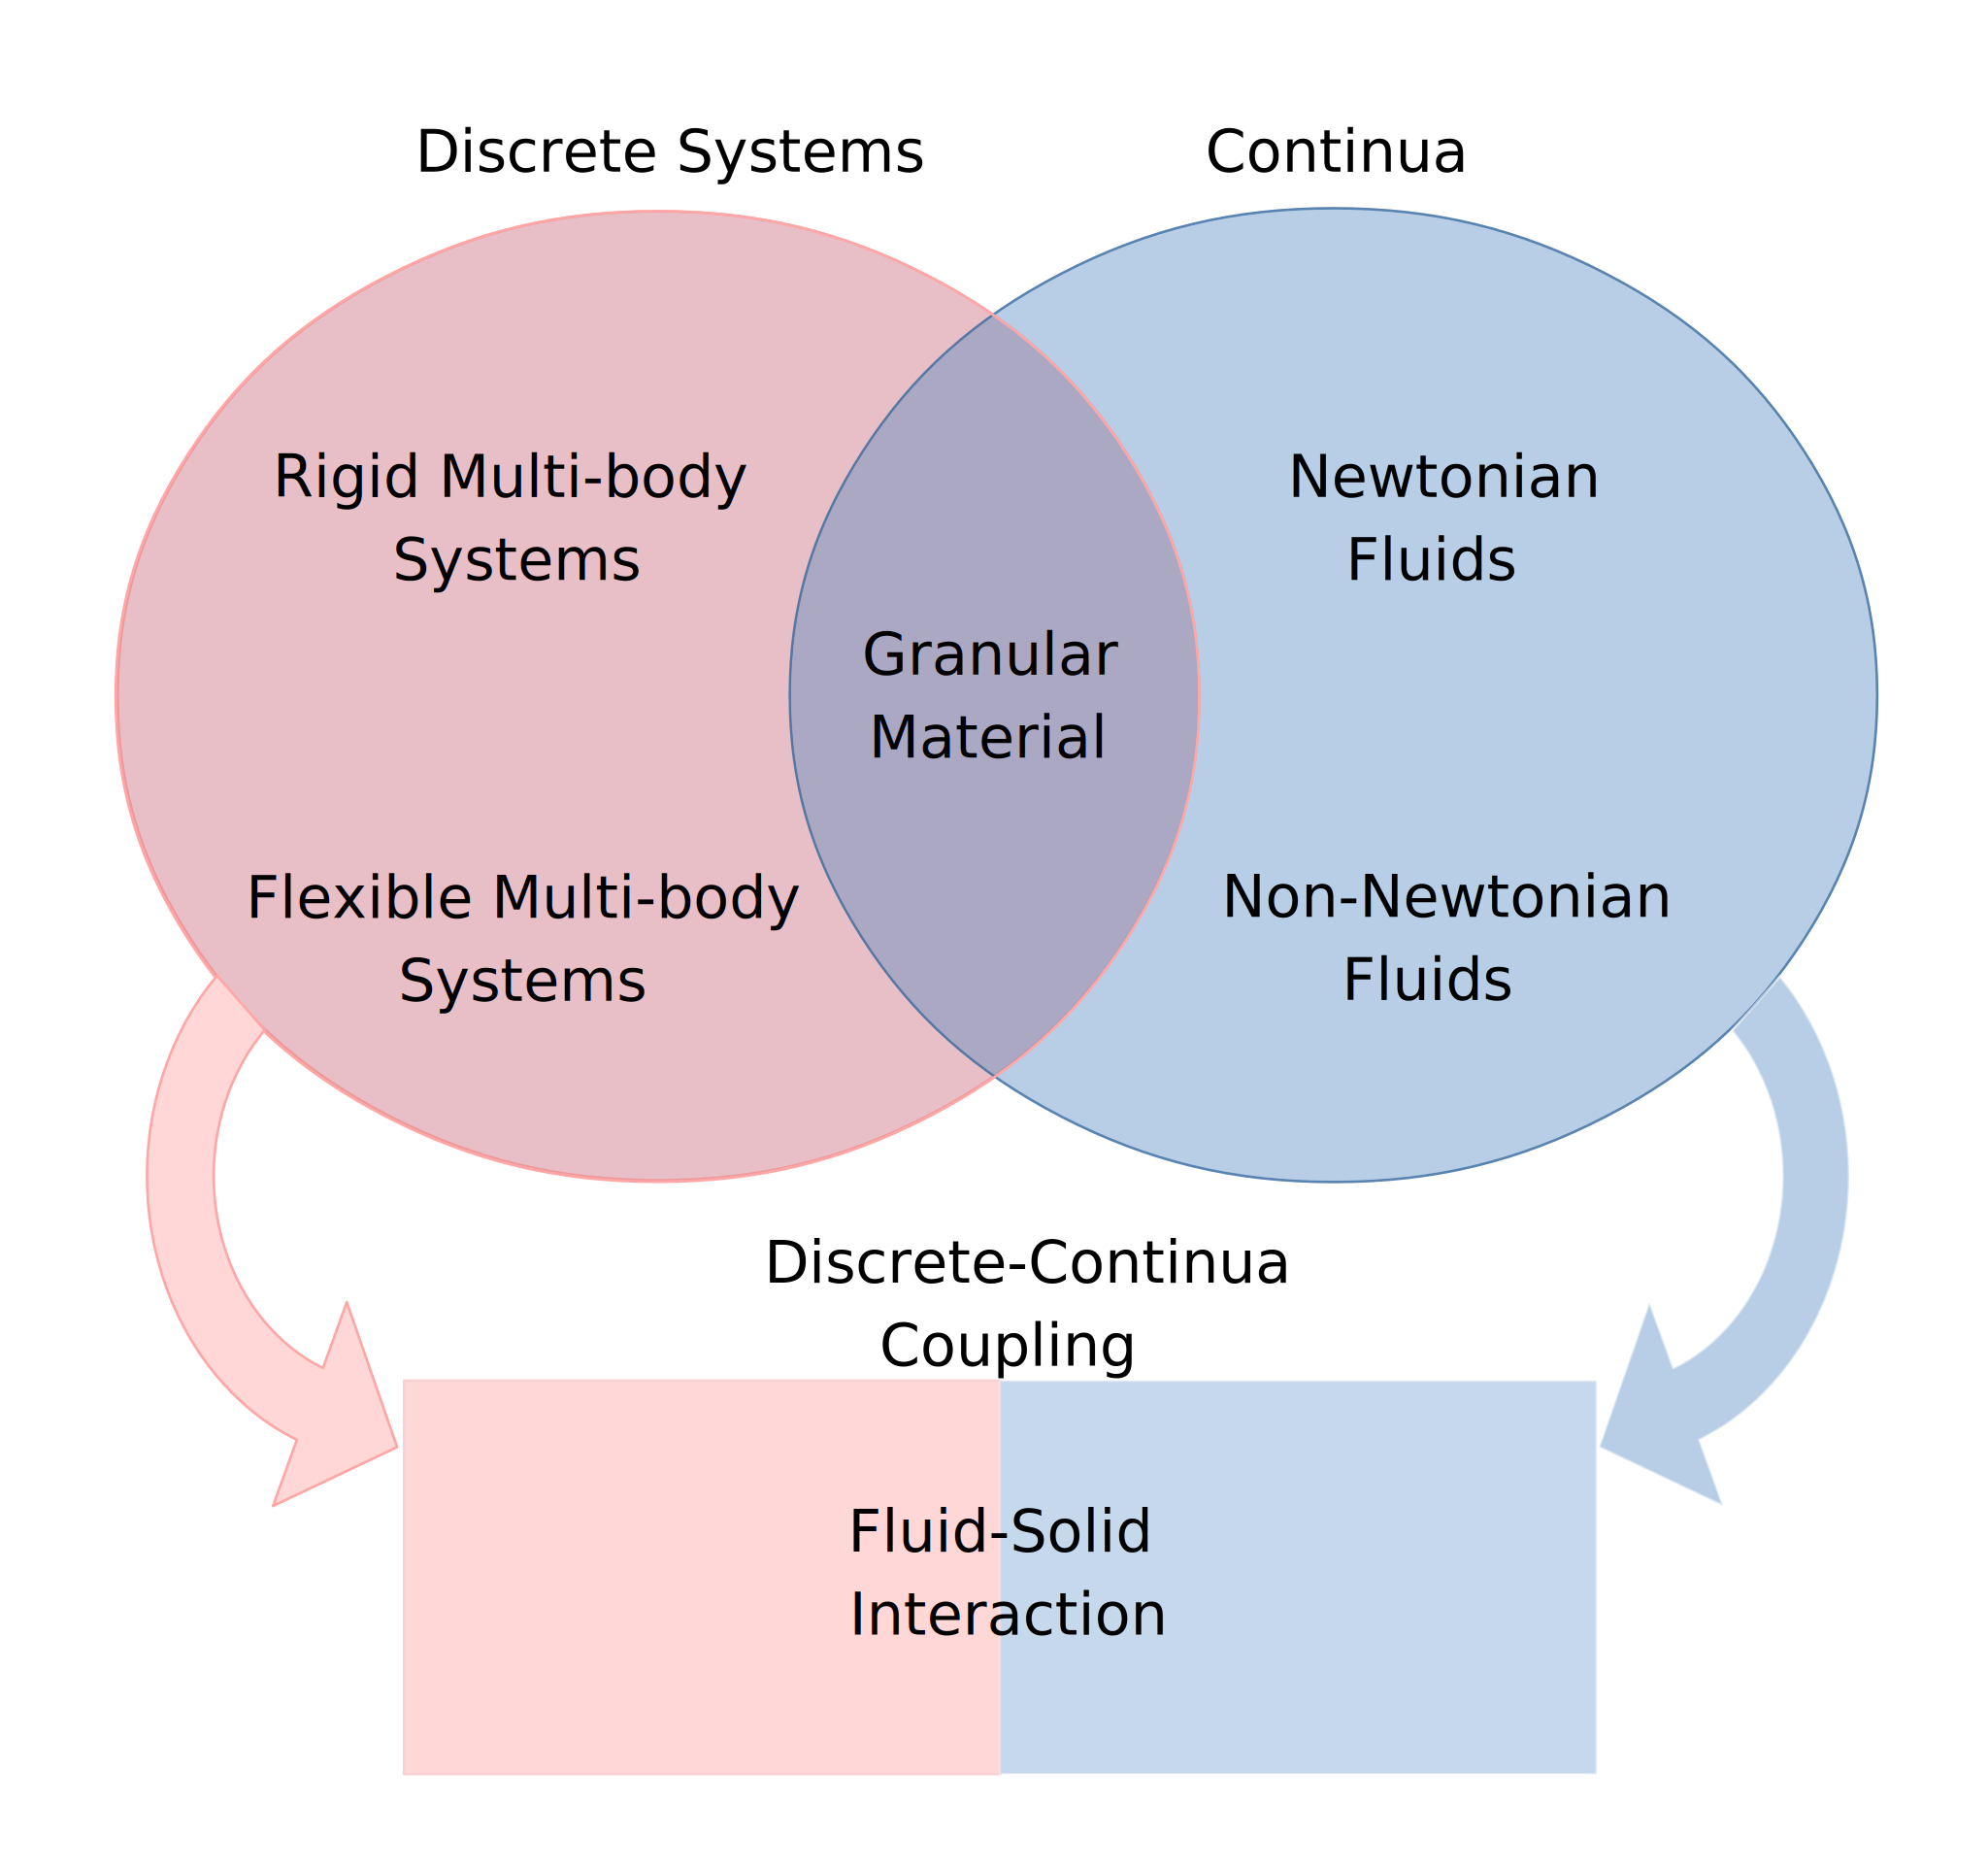
\includegraphics[width=.75\linewidth]{images/Overview.pdf}
	\end{center}
	\caption{Schematic overview of the problems of interest in the present thesis.}
	\label{fig:Overview}
\end{figure}


\section{Thesis Overview}
This manuscript is organized as follows: Chapter \ref{chap:background} will provide a brief overview of the existing work and literature on computational fluid dynamics, multi-body dynamics, and fluid-solid interaction. Chapters \ref{chap:discrete_Model} and \ref{chap:continua_Model} will discuss the modeling aspects and the numerical methods for solving the governing equations of discrete and continuous systems, respectively. Details about the software implementation of the  framework are presented in Chapter \ref{chap:implementation}, with numerical experiments and validation discussed in Chapter \ref{chap:experiments}. Chapter \ref{chap:demonstration} presents several applications and demonstrates the capabilities of the developed computational framework. Conclusions and directions of future work are discussed in Chapter \ref{chap:conclusions}.




\section{Summary of Contributions}
\label{sec:contributions}
The author's work has led to the following archival publications: \cite{miladSPHcomparison2019,lagrangianVSeulerian2019,miladHalfImplicit2018,rakhsha2019simulation,hammadConstrFluid2018,weiWenxiaoDanMultiresolution2017,miladASME2017}. The specific contributions of the author are summarized as follows:
\begin{compactitem} 
	\item Investigated the use of SPH for the Navier-Stokes equations
	\begin{compactitem} 
		\item Investigated four different SPH methods (WCSPH, ISPH, KCSPH, and IISPH) and  their solution attributes
		\item Performed a comparison between Implicit SPH (ISPH), Weakly Compressible SPH (WCSPH), and Kinematically Constrained SPH (KCSPH)
		\item Compared and contrasted the solution attributes of SPH as a Lagrangian method against continuous finite element method for free-surface and fluid-solid interaction problems 
		\item Implemented and improved the Implicit Incompressible SPH \cite{ihmsen2014implicit} method by solving the discretized Poisson pressure equation via advanced linear solvers
		\item Implemented and validated a projection-based implicit, both velocity and pressure, solver that can handle a wide range of fluid flows ranging from highly viscous flows to flows with moderately large Reynolds numbers in the laminar regime
		\item Investigated the use of consistent SPH discretization for internal flow problems
		\item Implemented the Herschel-Bulkley fluid model for modeling and simulation of non-Newtonian fluids
		\item Investigated the use of ISPH method for modeling and simulation of granular dynamics as a non-Newtonian fluid 
	\end{compactitem}
	

	\item Investigated the solution quality in frictional-contact problems and demonstrated insights gained in the context of a biomechanics application 
		\begin{compactitem} 
		\item  Investigated the use of the Tikhonov regularization method for imparting uniqueness to the distribution of frictional contact forces in granular dynamics problems solved via a differential variational inequality approach
		\item Simulated the tibiofemoral cartilage contact during walking for the prediction of collagen fiber orientation
	\end{compactitem}

	\item Developed a partitioned fluid-solid interaction framework
	\begin{compactitem} 
		\item  Coupled the fluid solver to a multi-body engine capable of simulating rigid and flexible bodies  interacting through frictional contact
		\item  Validated the fluid-structure coupling via benchmark experiments featuring flexible and rigid elements
	\end{compactitem}
	
	
	\item Leveraged hybrid CPU/GPU parallelization to improve the performance of the FSI framework 
	\begin{compactitem} 
		\item Implemented SPH on GPU cards using CUDA  to leverage high memory bandwidth
		\item Implemented Krylov linear solvers such as GMRES and BiCGStab on GPU to improve the efficiency of the underlying linear solvers
		\item Leveraged OpenMP for parallelism of the flexible multi-body dynamics solver on the CPU
		\item Improved the efficiency of the low-level matrix operation on the host code via AVX vectorization intrinsics
	\end{compactitem}
\end{compactitem} 
 %!TEX root = ../dissertation.tex

\chapter{Background}
\label{chap:background}
This chapter will provide brief background information about different types of physics studied in this manuscript. These include the dynamics of fluids, rigid and flexible multibody systems. Lastly, methods concerning the coupling between fluids and solids are discussed as well.

\section{Computational Fluid Dynamics}
Computational fluid dynamics is a significant branch of computational continuum mechanics, and it is concerned with the simulation of continua using computers. Many aspects of CFD have been studied in the past. This includes various space discretization and time integration schemes. Insofar as the space discretization step is concerned, the majority of CFD models can be classified as: $(i)$ Eulerian approaches, where the unknown state variables are attached to stationary observers; or $(ii)$ Lagrangian approaches, in which the unknown state variables are attached to moving observers.

Eulerian methods have been successfully applied and are very popular in CFD. Indeed, Finite Difference (FD) represents a robust technique for solving partial differential equations on simple domains, while the Finite Volume (FV) has been predominantly applied in fluid flows with complex geometries. Conversely, the Lagrangian methods gained traction only about two decades ago, although the idea of using Lagrangian discretization dates back to 1957 \cite{PIC}. Among Lagrangian methods, SPH  \cite{Lucy1977,Gingold1977} has been widely adopted as the low-order approximation of choice for a variety of problems \cite{Monaghan2005a}, while Moving Least Squares and Radial Basis Functions emerged as the leading high-order meshless methods \cite{trask2016compact,hu2019spatially,trask2018compatible,kansa1990scattered}. 

For FSI problems, just as for free-surface flows, the Eulerian approaches are challenged by large mesh deformations, which call upon re-meshing operations. A widely used approach is the Arbitrary Lagrangian-Eulerian (ALE) method \cite{ALE1974}, which handles well sufficiently small mesh deformation, yet it becomes expensive when the motion of the solid objects is relatively large. The Immersed Boundary Method (IBM) \cite{Peskin1977} addresses this shortcoming by implicitly treating the solid objects, as opposed to the ALE explicit representation of solid bodies that calls for body-fitted meshing. Thus, IBM alleviates the mesh deformation problem at the cost of a higher mesh resolution in the vicinity of the solid objects. 

Handling FSI problems comes more naturally to meshless methods, e.g. SPH, owing to their Lagrangian nature that interfaces well with the Lagrangian framework used in solid mechanics. However, SPH-based methods generally have enjoyed a somewhat limited adoption due to their reduced order and deficiencies in numerical approximation near boundaries \cite{trask2016compact}. Kernel-correction methods have been recently proposed to enforce linear consistency and second-order accuracy, yet they alter the conservation properties of SPH \cite{fatehi2011,Libersky1993,randles1996,Trask2015,islam2018consistency}. Likewise, the use of larger support basis functions improves robustness but leads to a higher computational cost.

Amongst different choices of discretization methods, in this thesis, SPH is embraced for space discretization of the underlying equations owing to its strength in solving free-surface, large-deformation, and fluid-solid interaction problems. SPH comes in many different formulations as far as time-integration, compressibility level, and boundary condition treatment are concerned, which will be further discussed in later chapters.



\section{Computational Multibody Dynamics}
A multibody system is defined as a collection of bodies interacting through mechanical constraints and frictional contact between the objects. Joints constrain the relative motion of bodies while springs and dampers induce additional loads in the system. Each body posses a specific mass and shape while the interconnects are treated as massless. These modeling assumptions apply to a large class of mechanical systems, from robots and vehicles to biomechanical systems \cite{simeon2013computational}. Computational multibody dynamics is the term used herein to refer to the numerical modeling technique used for resolving the dynamics of these discrete systems. Depending on the stiffness of discrete objects being studied, multibody systems may be further categorized into rigid multibody systems and flexible multibody systems.
\subsection{Rigid Multibody Systems}\label{sec:back_rigid}
A large body of literature is dedicated to rigid multibody systems featuring mechanical joints/constraints \cite{Haug89,shabana2013}. When frictional-contact between objects  is present, existing methods may be categorized in two groups: \textit{penalty} and \textit{complementarity} methods.

In penalty methods, the fundamental assumption is that bodies, although being rigid, deform slightly at the point of contact. The inter-penetration between the rigid bodies calculated during the proximity-computation stage is used to penalize further inter-penetration by creating contact forces between bodies through fictitious springs and dampers \cite{cundall71,cundall79,cundall1988formulation}. The process of choosing the model parameters and the simplification of the contact geometry are two main drawbacks of this method. Despite its shortcomings, penalty method has been used in numerous numerical studies on the dynamics of large rigid body systems \cite{Jaeger1996,brilliantov1996model,vu1999elastoplastic,vu2004accurate,luding2005,poschel2005computational}.

In the complementarity (constraint-based) approach, the main idea is to modify the equations of motion to include a differential inclusion \cite{filippov1967classical} and to impose non-penetration between rigid bodies through constraints enforced by applying impulses.  This method has been modified to model rolling and spinning friction in addition to sliding friction \cite{AleMihaiFriction2013}.  An important drawback associated with this method is the lack of uniqueness in the set of contact forces resulting from the solution of an optimization problem. In the present work, the complementarity method is employed to resolve the dynamics of contact between rigid bodies, while the penalty approach is used to handle contact between deformable bodies.


\subsection{Flexible Multibody Systems}
Unlike the rigid body dynamics where there is no distinction between the kinematics of the body and its reference frame, further modeling is required to capture the deformation of elastic components in flexible body dynamics. This is mainly because the distance between two points on/inside a deformable body changes, and the kinematics of the reference frame cannot sufficiently describe the time evolution of the flexible component. To this end, elastic components are discretized in space to study their motion via a \textit{finite} number of degrees of freedom. This is in contrast to rigid multibody systems where each rigid object is uniquely defined, regardless of its shape, by a set of position and orientation degrees of freedom. The final stage of the solution consists of solving for state variables, including those associated with rigid body motion as well as those defining elastic displacements and/or position and orientation of the discretized nodes.  The Floating Frame of Reference (FFR), co-rotational formulation, and Absolute Nodal Coordinate Formulation (ANCF) are three of the most relevant formulations in the context of flexible multibody systems. 


In the FFR formulation, the position of a point in the flexible body is expressed as the superposition of a small (flexible) \textit{deformation}, described in the body coordinate system, and possibly large \textit{translation} and \textit{rotation} of the body's coordinate system. The deformation of the body with respect to its coordinate system is expressed via the nodal coordinates of the discretized finite elements. The finite element used in the FFR formulation leads to zero strain under any arbitrary rigid body motion of the flexible object. Despite being the most widely used formulation in the computational flexible body dynamics, FFR is limited to cases where the deformation of the flexible body with respect to its reference frame is small. See \cite{Shabana1997,TR-2016-05-Recuero} for more details about the FFR formulation.  

The ANCF is a non-linear finite element method formulated to handle large deformations. In ANCF, no co-rotated frame is used to describe the kinematics of deformed finite elements. Most importantly, the distinguishing feature of ANCF is the use of position vector gradients to describe the rotation of the body as well as its strain state, thereby avoiding the need for interpolating non-vectorial rotation parameters. Given the interest of the present work in problems featuring large deformations and driven by the limitations of the FFR for such problems, the ANCF method is chosen in the present work. 


\section{Fluid-Solid Interaction}\label{sec:FSI_intro}
Many engineering applications, e.g., cardiovascular flows, fluid sloshing, particles in suspension, etc., require the solution of an FSI problem. Some of these problems involve large deformations, in which case the fluid-solid coupling remains challenging to solve \cite{ryzhakov2010}. For most FSI problems, it is nearly impossible to obtain analytical solutions. Additionally, laboratory experiments are also limited and costly to conduct \cite{hou2012}. Thus, numerical simulations must be employed. Different classifications exist in the context of numerical methods for FSI problems.

One classification is to consider the computational domain and divide the methods into \textit{conforming mesh methods} and \textit{non-conforming mesh methods}. In the conforming mesh methodology, the computational domains of sub-systems match at the interface, while in non-conforming mesh methods the computational domain of the fluid sub-system serves more as a background mesh for the solid phase. As an example of non-conforming mesh methods, in IBM \cite{peskin2002,mittal2005immersed}, the immersed boundary is tracked in a Lagrangian fashion; the fluid is tracked in an Eulerian framework on a non-conforming and regular grid; lastly, the presence of the immersed boundary on the non-conforming grid is included in Navier-Stokes equations as extra source terms. Fig.~\ref{fig:FSI_lit} illustrates the difference between the computational domains of the aforementioned methods. The approach to be taken in the current work does not fit into this classification since a mesh-less method is to be used for the fluid phase. However, the methodology is more similar to conforming mesh methods.

\begin{figure}[t!]
	\centering
	\begin{subfigure}[t]{0.4\textwidth}
		\centering
		\includegraphics[width=1\linewidth]{images/IBM.png}
		\caption{Non-conforming mesh method in IBM}
	\end{subfigure}%
	~ 
	\begin{subfigure}[t]{0.5\textwidth}
		\centering
		\includegraphics[width=1\linewidth,height=0.8\linewidth]{images/ConformingMesh.png}
		\caption{Conforming mesh method}
	\end{subfigure}
\caption{Illustration of the computational domains for non-conforming and conforming mesh methods.}
\label{fig:FSI_lit}
\end{figure}

Another classification pertains to the sequence of the solution algorithms and the governing equation of the overall system. Accordingly, FSI methods are grouped  into \textit{monolithic} and \textit{partitioned} approaches. In the former \cite{hubner2004,ryzhakov2010,michler2004}, the governing equations of the fluid and the solid phases are solved simultaneously; the interfacial conditions are implicit in the solution procedure; and potentially a better accuracy can be obtained for a multidisciplinary problem \cite{hou2012}. In contrast, in the latter approach, the two phases are solved separately, and the solutions are usually explicitly coupled together. Each method has its advantages and drawbacks. What makes the partitioned approach appealing is the fact that it solves each phase with efficient techniques that make the most out of the state-of-the-art methods in modeling, numerical solvers, and hardware architectures. Among partitioned methods, the ALE approach for the fluid and Lagrangian one for the solid are commonly used to treat strongly-coupled FSI problems \cite{hughes1981,souli2000}. In the ALE approach, the fluid mesh is deformed to adapt to the solid domain deformation \cite{fourey2010}. Although this approach has proven capable of handling  FSI problems with large-deformations, it is computationally expensive due to continuous mesh adaptation, a task that is not needed in meshless Lagrangian methods such as SPH \cite{yang2012}. 


Some recent FSI schemes resolve both the solid and the fluid dynamics in an Eulerian framework \cite{valkov2015eulerian,kamrin2012reference, liu2001eulerian,miller2002conservative}. The difficulty of computing the deformation gradient in an Eulerian framework is circumvented by tracking a reference map \cite{valkov2015eulerian,kamrin2012reference} or direct evolution of the deformation gradient as a field variable \cite{liu2001eulerian}. A distinct advantage of this class of methods is that all the phases are resolved by sweeping through a single mesh. On the downside, these methods are challenged by FSI problems involving contact between a large number of solid bodies as the computation of contact forces requires two level-set field variables per contact. Storing these field variables becomes expensive in comparison to $O(1)$ state variables that are stored in Lagrangian formulations \cite{valkov2015eulerian} for each contact.

In the present research, the Fluid-Solid Interaction method will be resolved in a Lagrangian-Lagrangian framework. Similar fluid-structure coupling was discussed in \cite{attaway1994} and further improved in \cite{fourey2010,Vuyst2005,groenenboom2010}. In \cite{attaway1994}, the contact forces were calculated based on an iterative master-slave scheme, which finds the best penalty forces required for the no-penetration condition. A similar but non-iterative scheme was used in \cite{groenenboom2010}. In \cite{fourey2010,armanCompFluids2015}, a dummy-particles scheme was used to compute the pressure from the fluid side. The present work follows in the footsteps of this last approach. 







\section{Granular Flows}\label{sec:back_granular}
While water is the most handled industrial material, granular material is the second.  Dense granular flows, however, are substantially more complex than their fluid counterparts. Granular material is essentially a discrete system whose evolution is described by the Newton-Euler's equations featuring frictional contact force (see Eq.~\ref{eq:Newton_Euler}). Although the discrete representation can accurately capture the motion of granular flows, the fully resolved modeling of large scale granular flows is a challenging task owing to $(i)$ their complex frictional contact interactions, and $(ii)$ a high computational burden as the motion of individual particles needs to be tracked in a numerical integration framework that advances simulation at time steps $\Delta t \approx 10^{-5}$ or lower. To address the latter aspect, discrete granular flow simulations use parallel computing to accelerate the computations. To date, the largest granular dynamics simulation of practical relevance contained 2.4 billion bodies, which was run on 16,384 CPUs (131,072 cores) of Japan's K-computer \cite{billBodyDEMJapanSC2017,japanDEMlarge2018}, the 2012 fastest supercomputer in the world and now the 18th in the ranking of the world's supercomputers \cite{TOP500}.

The collective behavior of individual particles may, however, be regarded as a continuum. Given that granular media can demonstrate distinctively different behaviors under various local stress conditions, the focus of this research is on the fluid-like evolution of granular material that happens when it is rapidly sheared. In such cases, $(i)$ shear stress in granular material shows strain-rate dependency, which is a characteristic of fluids and, $(ii)$ there exists a threshold value (yield criterion), under which the grains do not flow, a characteristic of solid materials. These features suggest a viscoplastic behavior of a granular material which is similar in nature to that of non-Newtonian fluids such as Bingham liquids \cite{jop2006constitutiveNature,campbell1990rapid}. 

Constitutive laws that could describe the motion of granular flows are still lacking. Amongst various models and theories developed previously, the $\mu(I)$-rheology \cite{jop2006constitutiveNature} is one of the successful frameworks describing observations from a variety of experimental and numerical results.

In the present work, we describe the fully resolved modeling of granular flows via the complementarity approach described in \S\ref{sec:back_rigid}.
  

\chapter{Discrete Systems}\label{chap:discrete_Model}
Contrary to continua, in discrete systems the motion of individual objects in the system and their interactions on each other is studied. In the following section, the mathematical formulations of such systems are described.
\section*{Definitions}
%For a reference on the notations used in the following sections, please see Chapter \ref{chap:nomenclature}.
Throughout section \S\ref{chap:discrete_Model}, the following conventions are used to denote the quantities associated with discrete systems. Scalar variables are denoted by uppercase or lowercase lightface Latin and Greek letters, e.g. $\rho$ and $\phi$. Vectors are denoted via bold, lowercase Latin letters, e.g. $\vect{x}$ and they are column vectors unless otherwise specified. More specifically, the variables $\vect{x}$, $\vect{v}$, $\vect{a}$ are used to represent the position, velocity and acceleration of an object. Indexed vectors are used to specify either an element of the vector or an object in the vector depending on the context, e.g. $\vect{x}_i$ is the position of body $i$. The first time-derivative is represented with over dot, e.g. $\dot{\vect{x}} = \vect{v}$.  The second time-derivative is denoted via over double-dot, e.g. $\ddot{\vect{x}} = \dot{\vect{v}} = \vect{a}$.  Matrices are represented as bold uppercase Latin letters, e.g. $\matr{M}$. One subscript is used to specify a single row, e.g. $\matr{M}_i$ for row $i$ in the matrix $\matr{M}$. Two subscripts are used to indicate a specific row and column, e.g. $\matr{M}_{i,j}$.   
The Frobenius norm of a matrix or a vector is defined as $\|*\|_F$. The skew-symmetric cross product operator for a three dimensional vector is defined as follows and results in a $3\times 3$ matrix
\begin{equation}
\tilde{{\vect s}} = \begin{bmatrix}
0 & -{s}_z & {s}_y\\ 
{s}_z & 0 & -{s}_x\\ 
-{s}_y & {s}_x & 0.
\end{bmatrix}
\end{equation}
\section{Rigid Body Dynamics}\label{sec:RigidBody}
In this section we describe the dynamic systems featuring rigid bodies and frictional contact between them. As explained in Section \S\ref{sec:back_rigid}, a complementarity-based approach is used to resolve the contact between different objects. 

\subsection*{Preamble}
``Rigid body'' refers to a 3D object that can translate and rotate in space. The set of generalized coordinates that describe the position and orientation of a body in the 3D Euclidean space are $\br_j\in \mathbb{R}^3$ and $\vect{\epsilon}_j\in \mathbb{R}^4$, which are respectively the absolute position of the center of mass, and Euler parameters associated with orientation of body $j$. Combining the set of generalized coordinates of different bodies for a system of $n_b$ bodies, one can write the set of generalized coordinates describing the system at position level as $\vect{x} = \left[ \vect{r}_1^T, \vect{\epsilon}_1^T,\ldots,\vect{r}_{n_b}^T, \vect{\epsilon}_{n_b}^T \right]^T \in \mathbb{R}^{7 n_b} $, and at velocity level as  $\dot{\vect{x}} = \left[ \dot{\vect{r}}_1^T, \dot{\vect{\epsilon}}_1^T,\ldots, \dot{\vect{r}}_{n_b}^T, 
\dot{\vect{\epsilon}}_{n_b}^T \right]^T$ $\in \mathbb{R}^{7 n_b}$. One can choose to use angular velocities instead of the time derivative of the Euler parameters to describe the system at the velocity level by  $\vect{v} = \left[ \dot{\vect{r}}_1^T, \bar{\vect{\omega}}_1^T,\ldots, \dot{\vect{r}}_{n_b}^T, 
\bar{\vect{\omega}}_{n_b}^T \right]^T$ $\in \mathbb{R}^{6 n_b}$, which reduces the problem size. The transformation from the derivatives of Euler parameters, ${\dot{\vect{\epsilon}}}_{B}$, to angular velocities at the body-fixed frame, ${\bar{\vect{\omega}}}_{B}$, for each body is governed by ${\dot{\vect{\epsilon}}}_{B}=\frac{1}{2} {\matr{G}}^T(\vect{\epsilon}_{B}) {\bar{\vect{\omega}}}_{B} $, where matrix ${\matr{G}}\in {\mathbb{R}}^{3 \times 4}$ depends linearly on the Euler parameters ${\vect{\epsilon}}_{B}$. Therefore, if one chooses to work with Euler angles at the velocity level, the block diagonal matrix  ${\vect L}(\vect{q}) \equiv \mbox{diag} \left[{{\matr I}}_{3 \times 3}, \frac{1}{2} {\matr{G}}^T(\vect{\epsilon}_{1}),\ldots,{\matr I}_{3 \times 3}, \frac{1}{2} {\matr{G}}^T(\vect{\epsilon}_{n_b})\right] \in {\mathbb{R}}^{7 n_b \times 6 n_b}$ can be used to obtain ${\dot{\vect{x}}} = {\vect L}({\vect{q}}) \vect{v}$, the time derivative of the set of generalized coordinate describing the system, where ${\matr I}_{3 \times 3}$ is the identity matrix \cite{Haug89}. 
\subsection{Bilateral Constraints}
A bilateral constraint represents a kinematic relationship between generalized coordinates in a discrete system. Spherical joints, prismatic joints, or revolute joints are examples of mechanical constraints that are comprised of a set of bilateral constraints represented by  $\mathcal{B}$. Hence, $\vect{g}_i\left(\vect{q},t\right)=\vect{0},i\in \mathcal{B}$ is a set of scalar equations to enforce kinematic constraints through algebraic equality equations. For instance, a revolute joint imposes five constraint equations, while a spherical is comprised of three constraint equations \cite{Haug89}.

The velocity-level constraint equations which must be satisfied are obtained by taking time-derivative of the constraints as  $\nabla_q \vect{g}_i^T \matr{L}\left(\vect{q}\right)\vect{v}+\dfrac{\partial\vect{g}_i}{\partial t}=0$.

\subsection{Unilateral Constraints and Frictional Contact}\label{sec:DVI}
In the Differential Variational Inequality (DVI) \cite{pastew03dvi} approach the equations of motion are modified to include a differential inclusion \cite{filippov1967classical} and to impose non-penetration between rigid bodies through constraints enforced by applying impulses. After discretization this problem is posed as an optimization problem with complementarity and equilibrium constraints. More specifically, the three-dimensional Coulomb friction assumption leads to a Non-linear Complementarity Problem (NCP).  In what follows, more details about the theory of the complementarity approach are explained.

Consider a contact between bodies $A$ and $B$ as shown in Fig.~\ref{fig:DVI_Contact}. The tangent plane at the contact point for the contact $i$ is defined by vectors $\textbf{u}_i$, $\textbf{w}_i$ and the normal $\textbf{n}_i$ in Fig.~\ref{fig:DVI_Contact}. A local reference frame can be defined for each body at the contact point based on these vectors. For body $A$, the normal to the tangent plane, $\textbf{n}_{i,A}$, points toward body $B$. The two mutually orthogonal vectors $\textbf{u}_{i,A}$, and $\textbf{w}_{i,A}$ are defined using the Gram-Schmidt method. The same methodology is used to build the local reference frame at the contact point $i$, for body $B$ with $\textbf{w}_{i,B}$, $\textbf{u}_{i,B}$, and $\textbf{n}_{i,B}$ $\in \mathbb{R}^3$. 

\begin{figure}
	\begin{center}
		\includegraphics[width=.4\linewidth]{images/twobodies.png}
	\end{center}
	\caption{Schematic of contact between two bodies.}
	\label{fig:DVI_Contact}
\end{figure}

If the gap (distance) between bodies $A$ and $B$ at the contact point is defined by $\Phi$, a complementarity condition can be defined as $0 \leq \widehat{\gamma}^c_{i,n}  \perp \Phi \geq 0$, where $\widehat{\gamma}^c_{i,n}$  is the Lagrange multiplier associated with the contact $i$. The complementarity condition states that at least one of the $\widehat{\gamma}^c_{i,n}$, or $\Phi$ is zero; when the gap function is zero, the normal contact force is greater than zero and when the normal contact force is zero the gap function is greater than zero (there is no contact between body $A$ and $B$). The contact force associated with contact $i$ can be expressed as $\vect{f}_{i,N}=\widehat{\gamma}^c_{i,n}\vect{n}_i$, and $\vect{f}_{i,T}=\widehat{\gamma}^c_{i,u}\vect{u}_i+\widehat{\gamma}^c_{i,w}\vect{w}_i$ which are the normal and tangential forces, respectively.  $\widehat{\gamma}^c_{i,w}$, $\widehat{\gamma}^c_{i,u}$, and $\widehat{\gamma}^c_{i,n}$ are the magnitude of the contact forces in each direction. The Coulomb dry-friction model based on the friction forces is expressed as  \cite{StTr95,stewartSIAMreview2000}
\begin{subequations}
	\begin{align}
	\label{eq:FrictionModel_1}
	\sqrt{(\widehat{\gamma}^c_{i,u})^2+(\widehat{\gamma}^c_{i,w})^2}\leq \mu^f_{i} \widehat{\gamma}^c_{i,n}&,\\ 
	\label{eq:FrictionModel_2}
	\quad \lVert\vect{v}_{i,T}\rVert\left(\sqrt{(\widehat{\gamma}^c_{i,u})^2+(\widehat{\gamma}^c_{i,w})^2} - \mu^f_{i} \widehat{\gamma}^c_{i,n} \right)=0&,\\
	\label{eq:FrictionModel_3}
	\langle\vect{f}_{i,T},\vect{v}_{i,T}\rangle=-\lVert\vect{f}_{i,T}\rVert\lVert\vect{v}_{i,T}\rVert \;&,
	\end{align}
\end{subequations}
where $\vect{v}_{i,T}$ denotes the relative tangential velocity between bodies $A$ and $B$ at the contact point. More specifically, Eq.~\ref{eq:FrictionModel_1} states that the the friction force is less than the normal force times the friction coefficient.  Eq.~\ref{eq:FrictionModel_2} states a complementarity condition where equality condition of Eq.~\ref{eq:FrictionModel_1} holds if the $\vect{v}_{i,T}\not=0$, and inequality of Eq.~\ref{eq:FrictionModel_1} holds if $\vect{v}_{i,T}=0$. Lastly, Eq.~\ref{eq:FrictionModel_3} states that the friction force is in the opposite direction of $\vect{v}_{i,T}$. If now one considers the following constraint minimization problem, 
\begin{equation}
\label{eq:fricMin}
\left( \widehat{\gamma}^c_{i,u},\widehat{\gamma}^c_{i,w} \right) = \mathop {\mbox{argmin}}\limits_{\sqrt{(\widehat{\gamma}^c_{i,u})^2+(\widehat{\gamma}^c_{i,w})^2} \leq \mu^f_{i} \widehat{\gamma}^c_{i,n}}
{\mathbf v}_{i,T}^T \left( \widehat{\gamma}^c_{i,u} \uVec{i} + \widehat{\gamma}^c_{i,w} \wVec{i} \right),
\end{equation}
then Eq.~\ref{eq:FrictionModel_1}-\ref{eq:FrictionModel_3} represent the first order Karush-Kuhn-Tucker optimality condition for the above optimization problem with respect to $\widehat{\gamma}^c_{i,u}$, and $\widehat{\gamma}^c_{i,w}$ variables. Hence, the Coulomb friction model is implemented as a constraint optimization problem. Finally, the contact force at the $i^{th}$ contact point is expressed as $\vect{f}_i=\vect{f}_{i,N}+\vect{f}_{i,T}=\widehat{\gamma}^c_{i,n}\vect{n}_i+\widehat{\gamma}^c_{i,w}\vect{u}_i+\widehat{\gamma}^c_{i,w}\vect{w}_i \in \cone_i$,  where $\cone_i$ is a 3D cone of slope $\tan^{-1}(\mu^f_{i})$ and oriented along $\vect{n}_i$, i.e., $\cone_i=\{\left[x,y,z\right]^T \in \mathbb{R}^3 | \sqrt{y^2+z^2} \leq \mu^f_{i} x\}$.


The Newton-Euler equations of motion for the system \cite{StTr95} are expressed as:
\begin{equation}
\label{eq:Newton_Euler}
\begin{gathered}
\begin{array}{rcl}
{\mathbf{\dot q}}   & = &  {\bf L}({\mathbf{q}}){\bf v} \vspace{0.2cm},  \\ 
{\mathbf{M}} {\mathbf{\dot v}} & = &{\mathbf{f}}\left( {t,  {\bf q} , {\bf v} } \right) -\vect{g}_{\vect{q}}^T\left(\vect{q},t\right)\lambda  + \vspace{0.2cm} \sum\limits_{i\in \cA({\bf q},\delta)} \left( \hatGN{i} \Pn{i} + \hatGU{i} \Ptu{i}  + \hatGW{i} \Ptw{i}  \right) \vspace{0.2cm}, \\
0 & = & {\bf g}({\bf q},t)\vspace{0.2cm}, \\ 
i \in \cA({\bf q}(t),\delta)  &:&  0 \le \hatGN{i} \; \perp \; \Phi_{i}({\bf q}) \geq 0 \vspace{0.2cm}, \\
\left(\hatGU{i}, \hatGW{i} \right)  &=&  \mathop {\mbox{argmin}}\limits_{\sqrt{(\widehat{\gamma}^c_{i,u})^2+(\widehat{\gamma}^c_{i,w})^2} \leq \mu^f_{i} \widehat{\gamma}^c_{i,n}} {\bf v}^T \left( \widehat{\gamma}^c_{i,u} \Ptu{i} + \widehat{\gamma}^c_{i,w} \Ptw{i} \right) \;,
\end{array}
\end{gathered} 
\end{equation}
where  $\mathbf{f}(t,  {\bf q} , {\bf v} ) $ are the external forces, $\textbf{M}$ is the system mass Matrix, $\cA({\bf q},\delta)$  is the set of active and potential unilateral constraints based on the bodies that are mutually less than $\delta$ apart, and $\textbf{g}(\textbf{q},t)$ is the set of bilateral constraints acting on the system and $\vect{g}_{\vect{q}}^T\left(\vect{q},t\right)$ is the Jacobian of the constraints with respect to the generalized coordinates. Moreover, the tangent space generators 
$\Proj{i}=[\Pn{i}, \Ptu{i}, \Ptw{i} ] \in {\mathbbm{R}}^{6n_b \times 3}$ are defined as
%
\begin{equation}
\begin{gathered}
\Proj{i}^{T} =
\left[ 
{\bf 0} \;\; \ldots \;\; - {\bf A}_{i,p}^T \;\; { {\bf A}_{i,p}^T {\bf{A}}_A {\tilde {\bar {\bf{s}}}}_{i,A}}  
\;\; {\bf 0} \;\;  \ldots  \;\;  {\bf 0} \;\;
{\bf A}_{i,p}^T \;\; { - {\bf A}_{i,p}^T {\bf{A}}_B  {\tilde {\bar {\bf{s}}}}_{i,B}  }  \;\; \ldots \;\;{\bf 0}
\right] ,
\end{gathered} 
\end{equation}
%
where ${\bf{A}}_{i,p} = [\nVec{i}, \uVec{i}, \wVec{i} ] \in {\mathbbm{R}}^{3 \times 3}$ is the orientation matrix associated with contact $i$,
${\bf{A}}_A={\bf{A}}\left({\bf \epsilon}_A\right)$ and ${\bf{A}}_B={\bf{A}}\left({\bf \epsilon}_B\right)$ are the rotation matrices of bodies $A$ and $B$ respectively; the vectors ${\bar {\bf s}}_{i,A}$ and ${\bar {\bf s}}_{i,B} \in {\mathbbm{R}}^{3}$  represent the contact point positions in body-relative coordinates as shown in Fig.~\ref{fig:DVI_Contact}. More details about the solution algorithm, and time-stepping scheme of the this DVI problem may be found in \cite{StTr95,ani04,aniha03}.


\subsection{Time Integration}
In the following, the superscript $(n)$ is used to represent values at time-step $t^{(n)}$, e.g.,  $\vect{q}^{(n)}$ and $\vect{v}^{(n)}$ represent the position and velocity at time-step $t^{(n)}$ respectively.
$\vect{\gamma}_i=h\hat{\vect{\gamma}}_i$ denotes contact impulse for contact $i$. The time integrated equations of motion discussed in Eq.~\ref{eq:Newton_Euler} for a time step $h$ is as follows:
\begin{align}
\vect{q}^{(l+1)}=&\vect{q}^{(l)}+h \matr{L}\left(\vect{q}^{(l)}\right)\vect{v}^{(l+1)} \label{eq:DVI_EOM_DISC:1},\\
\matr{M}\left(\vect{v}^{(l+1)}-\vect{v}^{(l)}\right)=&h \vect{f}\left(t^{(l)},\vect{q}^{(l)},\vect{v}^{(l)}\right)-\vect{g}_{\vect{q}}^T\left(\vect{q}^{(l)},t\right)\lambda, \nonumber \\
+&\sum\limits_{i=1}^{N_c} \left( \vect{\gamma}_{i,n} \matr{D}_{i,n}^T + \vect{\gamma}_{i,u} \matr{D}_{i,u}^T + \vect{\gamma}_{i,w} \matr{D}_{i,w}^T \right),\label{eq:DVI_EOM_DISC:2}\\
\underbrace{\frac{1}{h}\vect{g}\left(\vect{q}^{(l)},t\right)}_{\text{stabilization term}}+&\vect{g}_{\vect{q}}^T\matr{L}\left(\vect{q}^{(l)}\right)\vect{v}^{(l+1)}+\vect{g}_t=\vect{0} \label{eq:DVI_EOM_DISC:3},\\
\text{for} \quad i=1,2,\ldots,N_c, \nonumber\\
0 \leq \underbrace{\frac{1}{h}\Phi_i\left(\vect{q}^{(l)},t\right)}_{\text{stabilization term}}+&\matr{D}_{i,n}^T\vect{v}^{(l+1)}  \underbrace{-\mu_i \sqrt{\left(\matr{D}_{i,u}^T\vect{v}^{(l+1)}\right)^2+\left(\matr{D}_{i,w}^T\vect{v}^{(l+1)}\right)^2} }_{\text{relaxation term}}\perp \vect{\gamma}_{i,n} \geq 0, \label{eq:DVI_EOM_DISC:4}\\
\left(\vect{\gamma}_{i,u},\vect{\gamma}_{i,w}\right)=&\argmin_{\sqrt{\vect{\gamma}_{i,u}^2+\vect{\gamma}_{i,w}^2}\leq \mu_i\vect{\gamma}_{i,n}} \left(\vect{\gamma}_{i,u}{\vect{v}^{(l+1)}}^T \matr{D}_{i,u}+\vect{\gamma}_{i,w} {\vect{v}^{(l+1)}}^T \matr{D}_{i,w}\right) \label{eq:DVI_EOM_DISC:5}.
\end{align}
Above, the position level update Eq.~\ref{eq:DVI_EOM_DISC:1} follows the forward Euler scheme. Eq.~\ref{eq:DVI_EOM_DISC:2} is the time-discretized momentum balance featuring the reaction forces associated with bilateral (mechanical) and unilateral (contact) constraints.  Eq.~\ref{eq:DVI_EOM_DISC:3} is time-discretized algebraic equation for bilateral constraints. Eq.~\ref{eq:DVI_EOM_DISC:4} is the time-discretized scalar complementarity condition in the normal direction while Eq.~\ref{eq:DVI_EOM_DISC:5} is the minimization problem corresponding to the Coulomb friction model for frictional forces. Inclusion of the relaxation term in Eq.~\ref{eq:DVI_EOM_DISC:4} leads to a Cone Complementarity Problem (CCP), which represents the first order optimality condition of a Quadratic Optimization with Conic Constraints (QOCC). It has been shown in \cite{ani04} that the solution of the modified scheme will approach the solution of the original problem as the step-size goes to zero.
The underlying CCP is as follows:
\begin{align}\label{eq:DVI_CCP}
&\text{Find } \vect{\gamma}_i, \text{ for } i=1,\ldots,N_c \nonumber, \\
&\text{such that } {\mathcal{K}}_i \ni \vect{\gamma}_i\perp -\left(\matr{N}\vect{\gamma}+\vect{r}\right)_i \in {\mathcal{K}}_i^\circ ,\\
&\text{where}\; {\mathcal{K}}_i=\{\left[x,y,z\right]^T \in \mathbb{R}^3 | \sqrt{y^2+z^2} \leq \mu_i x\} \nonumber,\\
&\text{and}\; {\mathcal{K}}_i^\circ=\{\left[x,y,z\right]^T \in \mathbb{R}^3 | x \leq -\mu_i\sqrt{y^2+z^2}\}, \nonumber
\end{align}
where the superscript $^{(l+1)}$ in $\vect{\gamma}_i=\vect{\gamma}_i^{(l+1)}$ was omitted for clarity. The system level coefficient Matrix $\matr{N}$ and the vector $\vect{r}$ are defined as:
\begin{eqnarray}
\matr{N}&=&\matr{D}^T\matr{M}^{-1}\matr{D}, \\
\matr{r}&=&\vect{b}+\matr{D}^T\matr{M}^{-1}\vect{k}.
\end{eqnarray}
Above,  $\vect{b}_i = \left[\frac{1}{h}\Phi_i,0,0\right]^T$ for contact $i$, and $\vect{k}=\matr{M}\vect{v}^{(l)}+h \vect{f}\left(t^{(l)},\vect{q}^{(l)},\vect{v}^{(l)}\right)$.

\noindent
The equivalent QOCC of the above problem is as follows:
\begin{eqnarray}\label{eq:DVI_QOCC}
&&\min f\left(\vect{\gamma}\right) = \frac{1}{2}\vect{\gamma}^T \matr{N} \vect{\gamma}+\vect{r}^T \vect{\gamma} \label{eq:OPT_friction},\\
&&\text{subject to } \vect{\gamma}_i \in {\mathcal{K}}_i \text{ for } i=1,2,\ldots,N_c, \nonumber
\end{eqnarray}
\noindent
where $\vect{\gamma}_i$ is the triplet of multipliers associated with contact $i$ and $\vect{\gamma}_i\in{\mathcal{K}}_i$  as stated in Eq.~\ref{eq:DVI_CCP}.
Herein,  $\vect{\gamma}=\left[\vect{\gamma}_1^T,\vect{\gamma}_2^T,\ldots,\vect{\gamma}_{N_c}^T\right]^T$ is the system level vector of Lagrange multipliers (contact impulses) associated with unilateral constraints. The equivalence of Eqs.~\ref{eq:DVI_CCP} and \ref{eq:OPT_friction} has been verified by considering the KKT first-order necessary conditions in \cite{heynPhDThesis2013}. Various methods exist for solving Eqs.~\ref{eq:DVI_CCP} and \ref{eq:OPT_friction}. In \cite{heynPhDThesis2013} advantages and shortcomings of solution algorithms such as Jacobi, Gauss-Siedel, Accelerated Projected Gradient Descent (APGD), and interior-point method for solution of the problem in its optimization form, Eq.\ref{eq:OPT_friction}, were discussed.

\subsection{Solution Uniqueness}\label{sec:Uniqueness}
The complementarity method discussed in Eqs.~\ref{eq:DVI_CCP} or \ref{eq:DVI_QOCC} for idealized perfectly-rigid bodies does not have a unique solution. Specifically, this is due to the indeterminacy of the curvature matrix $\matr{N}$, which is typically positive semidefinite. A positive semidefinite matrix $\matr{N}$ emerges when there are many contacts per body. Thus, the system has infinitely many sets of reaction forces that satisfy the DVI equations. This non-uniqueness appears only in the normal forces for frictionless problems, while both the velocities and the contact forces are non-unique for frictional problems. Use of additional compatibility conditions for contact forces in frictionless problems was investigated in \cite{olsen2018resolving}. The compatibility condition maintains no-penetration constraints but filters out force distributions that could not have arisen from stiff elastic contacts. In the present work, we use the Tikhonov regularization method to improve the solution quality in frictional problems. 
Herein, the set of solution to Eq.~\ref{eq:DVI_QOCC} is denoted by 
\begin{equation}
\mathcal{S} = \{ \vect{\gamma} \in {\mathcal{K}}  \;| \; f(\vect{\gamma}) = \inf_{\vect{y} \in \mathcal{K}} \; f(\vect{y}) \}, 
\end{equation}
where $\mathcal{K}=\mathcal{K}_1\times\mathcal{K}_2 \hdots \times \mathcal{K}_{N_c}$  is the direct product of the individual contact cones.

The Tikhonov regularized QOCC of Eq.~\ref{eq:DVI_QOCC}  is modified as:
\begin{eqnarray}\label{eq:DVI_QOCC_reg}
&&\min f_\alpha \left(\vect{\gamma}\right) = \frac{1}{2}\vect{\gamma}^T \matr{N} \vect{\gamma}+\vect{r}^T \vect{\gamma} + \alpha \|\vect{\gamma}\|^2_W  \label{eq:OPT_friction_ref},\\
&&\text{subject to } \vect{\gamma}_i \in {\mathcal{K}}_i \text{ for } i=1,2,\ldots,N_c. \nonumber
\end{eqnarray}
The inclusion of the regularization term $\alpha \|\vect{\gamma}\|^2_W$ increases the zero eigenvalues of the $\matr{N}$ to ensure a unique solution. Note that the cost function in Eq.~\ref{eq:DVI_QOCC_reg} is strictly convex for ${\alpha}>0$. 

According to the Tikhonov regularization method, the minimum-norm solution of a \textit{convex} optimization problem may be obtained by solving a sequence of related \textit{strongly convex} optimization problems. Accordingly, the sequence ${\vect{\gamma}_k}$ generated by the Tikhonov regularized problem
\begin{equation}
 \vect{\gamma}^{k+1} = \underset{\vect{\gamma} \in {\mathcal{K}} }{\mathrm{argmin}} \{\frac{1}{2}\vect{\gamma}^T \matr{N} \vect{\gamma}+\vect{r}^T \vect{\gamma} + \alpha_k \|\vect{\gamma}\|^2_W   \},
\end{equation}
 converges to the minimum norm of $S$ as $\alpha \to 0^+$, which is sufficient from the theoretical perspective. However, one may choose not to find the exact solution of each subproblem, but solving it withing some tolerance $\epsilon_k$, in order to make the solution procedure more efficient. The idea is to solve the subproblem with looser tolerances at the beginning and with more strict tolerances as $\alpha \to 0^+$. In practice, one may choose to reduce the tolerance and the regularization parameter as $\epsilon_{k+1}=\tau_{\epsilon} \epsilon_{k}$ and $\alpha_{k+1}=\tau_{\alpha} \alpha_{k}$, for some constants $\tau_{\alpha}$ and $\tau_{\epsilon}$, where $0<\tau_{\epsilon}<\tau_{\alpha}<1$. 
 
 Alternatively, one may choose a small value of the regularization parameter $\alpha_k$ and solve only one subproblem and since the feasible set is convex for $\alpha>0$. This regularized problem has a unique solution although the solution may slightly differ from the classical Tikhonov regularization method described above. These ideas are investigated for a few benchmark problems in section \S\ref{sec:DVI_Uniq}.

\section{Flexible Body Dynamics}\label{sec:FMBD}
The nonlinear flexible body dynamics formulation used in the current work draws on ANCF, a nonlinear finite element formulation introduced by Shabana~\cite{Shabana1997} to describe large deformation of moving bodies. The salient feature of ANCF is the use of position vector gradients to describe the rotation of the body. ANCF uses the nodal global-position and the nodal position-vector-gradients to describe the nonlinear dynamics of flexible bodies that can undergo large deformation.
In general, the position field of $i^{th}$ ANCF element may be defined as: 
\begin{equation} \label{eq:ANCF_r}
\underbrace{{{\bm{r}}^{i}}(\xi,\eta,\zeta,t)}_{\begin{smallmatrix}
	\text{Position of an arbitrary } \\
	\text{point within the element}
	\end{smallmatrix}}=\underbrace{\bm{S}(\xi,\eta,\zeta)}_{\begin{smallmatrix}
	\text{Space-dependent } \\
	\text{shape function}
	\end{smallmatrix}}\times \underbrace{{{\bm{q}}^{i}}(t),}_{\begin{smallmatrix}
	\text{Time-dependent vector of } \\
	\text{nodal degrees of freedom}
	\end{smallmatrix}}
\end{equation}
which simply gives the position of any point $(\xi,\eta,\zeta) \in [-1,1]$ inside the element at time $t$ based on interpolation ($\bm{S} (\xi,\eta,\zeta) $) of the nodal coordinates ($\bm{q}^{i}(t)$). Due to the fact that description of elements is in global coordinates, the inertia forces have a simple form in ANCF elements. The velocity of any point within an element $i$ may be written as
\begin{equation} \label{eq:ANCF_r_dot}
\underbrace{\bm{\dot{r}}^{i}(\xi,\eta,\zeta,t)}_{\begin{smallmatrix}
	\text{Velocity of an arbitrary } \\
	\text{point within the element}
	\end{smallmatrix}}=\underbrace{\bm{S}(\xi,\eta,\zeta)}_{\begin{smallmatrix}
	\text{Space-dependent } \\
	\text{shape function}
	\end{smallmatrix}}\times \underbrace{\bm{\dot{q}}^{i}(t).}_{\begin{smallmatrix}
	\text{Time-dependent vector of } \\
	\text{generalized velocities}
	\end{smallmatrix}}
\end{equation}
The kinetic energy of a finite element $i$ can be obtained as
\begin{equation} \label{eq:ANCF_T}
T = \frac{1}{2}\int\limits_V {\rho {{{\mathbf{\dot r}}}^{i\text{T}}}{\mathbf{\dot r}}^{i}} {\text{ d}}V = \frac{1}{2}{{\mathbf{\dot q}}^{i\text{T}}}{\mathbf{M\dot q}^{i}}\;,
\end{equation}
where the mass matrix ${\mathbf{M}}$ is defined as \small ${\mathbf{M}} = \int_A {\rho A {{\bm{S}}^\text{T}}{\bm{S}}} {\text{ d}}x$, which is time-independent. The equations of motion assume the form \cite{shabana2013} 
\begin{equation}
\mathbf{M} \ddot{\mathbf{q}} + \mathbf{{Q}}_e=\mathbf{{Q}}_a\;,
\end{equation}
where  $\mathbf{{Q}}_e$ and $\mathbf{{Q}}_a$ are the generalized element elastic and applied forces, respectively. The description of these elements and calculation of the internal forces are described in \S \ref{sec:1DElem}, and \S \ref{sec:2DElem}.

ANCF elements may be classified based on the number of position vector gradients defined at each node. ($i$) \textbf{Fully parameterized} ANCF elements use position vector $r \in \mathbb R^3$, and 3 position vector gradients, $\bm{r}_x$, $\bm{r}_y$, and $ \bm{r}_z  \in \mathbb R^3 $ where $x$, $y$, and $z$ are the natural coordinates of the element. Fully parameterized elements allow for easy implementation of the continuum mechanics approach to calculate the deformation gradient ($\textbf{F}$). ($ii$) \textbf{Gradient Deficient} ANCF elements use position vector $r \in \mathbb R^3$, and fewer than 3 position vector gradients, when using fewer position vector gradients is sufficient to define the volume used in continuum mechanics approach. Using fewer position gradient vectors has been shown to eliminate various locking problems.

Development of ANCF elements is still an ongoing research topic, yet in the current work elements that have been shown robust and acceptable accuracy are chosen for the simulations of the flexible bodies. More specifically, ANCF cable element, ANCF shell element, and hexahedron brick elements, which are appropriate respectively for modeling 1D, 2D, and 3D bodies, are to be used in the FE analysis of this present work.


\subsection{ANCF Cable Element}\label{sec:1DElem}
The gradient-deficient ANCF cable element introduced by Berzeri and Shabana~\cite{berzeri2000} is used in the present work. As shown in Fig.~\ref{fig:ANCFCable}, the coordinates of this element at each node are a position vector and a position vector gradient along the beam central axis. The position gradient vectors normal to the cable axis are not defined, hence the element is gradient deficient. Subsequently, torsion and shear deformation cannot be captured with this set of degrees of freedom. The coordinates (nodal degree of freedom) of the $j^{th}$ node is expressed as the $6 \times 1$ matrix \small${{\bm{q}}^{j}}(t)={{\left[ \begin{matrix}
		\bm{r}_{{}}^{j\text{T}} & \bm{r}_{x}^{j\text{T}}  \\
		\end{matrix} \right]}^{\text{T}}}$. \normalsize The position of any point inside the $i^{th}$ element may be interpolated from the nodal degrees of freedom of its nodes as follows
\begin{equation} \label{eq:ANCF_Beam_r}
\bm{r}^{i}=\left[ \begin{matrix}
{{s}_{1}}\bm{I} & {{s}_{2}}\bm{I} & {{s}_{3}}\bm{I} & {{s}_{4}}\bm{I}  \\
\end{matrix} \right]\left[ \begin{matrix}
\bm{q}_{}^{1\text{T}} & \bm{q}_{}^{2\text{T}}  \\
\end{matrix} \right]^\text{T}=\bm{S}\left( \xi  \right)\bm{q}^{i},
\end{equation}
where $\bI$ is the $3\times3$ identity matrix, $\bm{S}\left( \xi  \right)$ is a $3 \times 12$ matrix, $\bm{q}^1$, are $\bm{q}^2$ are the nodal coordinates of the two nodes forming element $i$, as defined before, and finally $\bm{q}^{i}$ is a $12\times1$ matrix combining the nodal coordinates of the element $i$. The interpolation functions are defined as
\begin{equation} \label{eq:ANCF_Beam_Shapefunctions}
\begin{split}
& {{s}_{1}}=1-2{{\xi}^{2}}+2{{\xi}^{3}}, \\
& {{s}_{2}}=l\left( \xi-2{{\xi}^{2}}+{{\xi}^{3}} \right), \\
& {{s}_{3}}=3{{\xi}^{2}}-2{{\xi}^{3}}, \\
& {{s}_{4}}=l\left( -{{\xi}^{2}}+{{\xi}^{3}} \right), \\
\end{split}
\end{equation}
where $0<\xi <1$ is the non-dimensional parameter defined over the natural coordinates of the element locates a point along the cable centerline ($\xi=0$ at the first node, and $\xi=l$ at the second node), and $l$ is the length of the element.

\begin{figure}[!t]
	\begin{center}
		\includegraphics[width=.6\linewidth]{images/ANCF_1D.png}
	\end{center}
	\caption{ANCF cable element's schematic. Each node features a global position vector and a position vector gradient along the axis of the element (6DOF). Using shape functions and knowing $\xi$ one can interpolate the degrees of freedom to any point $P$ within the element. } \label{fig:ANCFCable}
\end{figure}


Knowing the axial and bending strains, one can define the internal loads of this element. 
The generalized element elastic forces are calculated as follows:
\begin{equation} \label{eq:ANCF_Beam_Qe}
\mathbf{Q}^i_{e}=\int\limits_{L}{\left[ EA \varepsilon_{x} ({\frac{{\partial \varepsilon }_{x}}{\partial \mathbf{q}}})^T+EI\kappa ({\frac{\partial \kappa}{\partial \mathbf{q}}})^T  \right]}\text{d}x,
\end{equation}
where $E$, $A$, and $I$ are the modulus of elasticity, the cross section area, and the area moment of inertia, respectively. The axial strain and curvature are defined as follows
\begin{equation*} \label{eq:ANCF_Beam_ex_k}
{{\varepsilon }_{x}}=\frac{1}{2}\left( \bm{r}_{x}^{\text{T}}\bm{r}_{x}^{{}}-1 \right) \text{  } \text{and} \text{  } \kappa \text{=}\frac{\left| {{\bm{r}}_{x}}\times {{\bm{r}}_{xx}} \right|}{{{\left| {{\bm{r}}_{x}} \right|}^{3}}},
\end{equation*}
where $\bm{r}^i_{x}=\bm{S}_x(\zeta) \bm{q}^i$ and $\bm{r}^i_{xx}=\bm{S}_{xx}(\zeta) \bm{q}^i$ terms involve differentiation of the shape function matrix $\bm S$.

Similarly, external applied forces, including those coming from the fluid system are interpolated to nodal coordinates and subsequently applied in the structural system via:
\begin{equation} \label{eq:ANCF_Beam_Qa}
Q^i_a = \bm S(x)^T \bm F.
\end{equation}

The generalized body forces including gravity force may be computed according to the standard finite element formulation as :

\begin{equation} \label{eq:ANCF_Beam_Qb}
Q^i_b = \int_{L} \rho_s A \bm S(x)^T \bm f_b,
\end{equation}
where $\rho_s$ and $A$ are the density and cross sectional area of the element, and $f_b$ is density of the body force. 


\subsection{ANCF Shell Element}\label{sec:2DElem}
The gradient-deficient ANCF shell element studied in \cite{Yamashita2015continuum} is used in the present work to simulate 2D flexible bodies. The nodal global position vector ($\mathbf{r}^{i}$) and global position vector transverse gradient ($\mathbf{r}_{z}^{i}=\frac{\partial {{\mathbf{r}}^{i}}}{\partial {{z}^{i}}}({{\xi}^{i}},{{\eta}^{i}})$) are chosen as the nodal degrees of freedom, as shown in Fig.~\ref{fig:ANCF_Shells}.

\begin{figure}[!t]
	\begin{center}
		\includegraphics[width=.6\linewidth]{images/ANCF_2D.png}
	\end{center}
	\caption{ANCF shell element's schematic. Global position vector $\mathbf{r}^{j}$ and fiber's direction $\mathbf{r}_z^{j}=\frac{\partial {{\mathbf{r}}^{j}}}{\partial {{z}^{i}}}({{\xi}^{i}},{{\eta}^{j}})$ are the nodal coordinates of the $j^{th}$ node (6DOF). Using shape functions and knowing $\xi$ and $\eta$ one can interpolate the degrees of freedom to any point within the element. }\label{fig:ANCF_Shells}
\end{figure}

The positions and gradients on the mid-plane for any point inside the $i^{th}$ element can be interpolated from the positions and gradients of its nodes as follows
\begin{equation} \label{eq:ANCF_Shell_coordinates}
\mathbf{r}_{m}^{i}({{\xi}^{i}},{{\eta}^{i}})=\mathbf{S}_{m}^{i}({{\xi}^{i}},{{\eta}^{i}})\mathbf{e}_{p}^{i},\quad \frac{\partial {{\mathbf{r}}^{i}}}{\partial {{z}^{i}}}({{\xi}^{i}},{{\eta}^{i}})=\mathbf{S}_{m}^{i}({{\xi}^{i}},{{\eta}^{i}})\mathbf{e}_{g}^{i},
\end{equation}
where $\xi^i$ and $\eta^i$ refer to $i^{th}$ element's natural coordinates in the parametric space, $\mathbf{S}_{m}^{i}=\begin{bmatrix}
S_{1}^{i}\mathbf{I}& S_{2}^{i}\mathbf{I}& S_{3}^{i}\mathbf{I}&  S_{4}^{i}\mathbf{I}] \end{bmatrix}$ is a bilinear shape function matrix, $\mathbf{e}_{p}^{ij}={{\mathbf{r}}^{ij}}$ is the position vector of $j^{th}$ node of the element $i$, and $\mathbf{e}_{g}^{ij}={\partial {{\mathbf{r}}^{ij}}}/{\partial {{z}^{i}}}\;$ is the position vector gradient of node $j$ of element $i$, and $\textbf{I}$ is the $3\times 3$ identity matrix.
The bilinear shape functions of the ANCF shell element are given by the following expressions
\begin{equation*} \label{eq:ANCF_Shell_Shapefunctions}
\begin{split}
S_{1}^{i}=\frac{1}{4}(1-{{\xi }^{i}})(1-{{\eta }^{i}}), S_{2}^{i}=\frac{1}{4}(1+{{\xi }^{i}})(1-{{\eta }^{i}}),\\
S_{3}^{i}=\frac{1}{4}(1+{{\xi }^{i}})(1+{{\eta }^{i}}), S_{4}^{i}=\frac{1}{4}(1-{{\xi }^{i}})(1+{{\eta }^{i}}).
\end{split}
\end{equation*}
The position of an arbitrary point in the $i^{th}$ element may be described as
\begin{equation} \label{eq:ANCF_Shell_r}
{{\mathbf{r}}^{i}}({\xi}^i,{\eta}^i,{z}^i)={{\mathbf{S}}^{i}}({\xi}^i,{\eta}^i,{z}^i){{\mathbf{e}}^{i}},
\end{equation}
where ${{\mathbf{S}}^{i}}=[\begin{matrix} \mathbf{S}_{m}^{i} \,\,\, {{z}^{i}}\mathbf{S}_{m}^{i}\end{matrix}]_{3\times 24}$ is the combined shape function matrix, and $\quad {{\mathbf{e}}^{i}}= [{ \begin{matrix} {{(\mathbf{e}_{p}^{i})}^{T}} \,\,\, {{(\mathbf{e}_{g}^{i})}^{T}}\end{matrix}}]_{1\times 24}^T$ is the coordinates of the $i^{th}$ element grouped together. Eq.~\ref{eq:ANCF_Shell_r} allows for interpolating points along the element thickness by incorporating the element natural coordinate $z^i$.
The Green-Lagrange strain tensor, which is expressed as follows, 
\begin{equation} 
{{\mathbf{E}}^{i}}=\frac{1}{2}\left( {{\left( {{\mathbf{F}}^{i}} \right)}^{T}}{{\mathbf{F}}^{i}}-\mathbf{I} \right),
\label{eq:ANCF_E}
\end{equation}
is used to obtain the strains, where ${\mathbf{F}}^{i}$ is the deformation gradient matrix defined as the Jacobian of the current configuration over the reference configuration, which is expressed as 
\begin{equation} 
{{\mathbf{F}}^{i}}=\frac{\partial {{\mathbf{r}}^{i}}}{\partial {{\mathbf{X}}^{i}}}=\frac{\partial {{\mathbf{r}}^{i}}}{\partial {{\mathbf{x}}^{i}}}{{\left( \frac{\partial {{\mathbf{X}}^{i}}}{\partial {{\mathbf{x}}^{i}}} \right)}^{-1}}=  \bar {\bm J}^i  ({\bm J^i})^{-1}, \label{eq:ANCF_F}
\end{equation}
where $\dfrac{\partial {{\mathbf{r}}^{i}}}{\partial {{\mathbf{x}}^{i}}}=\bar {\bm J}^i$, and ${{ \dfrac{\partial {{\mathbf{X}}^{i}}}{\partial {{\mathbf{x}}^{i}}} }}= {\bm J^i}$. Incorporating \ref{eq:ANCF_F}, in \ref{eq:ANCF_E} results in
\begin{equation}
\bm{E}^i=({\bm{J}^i})^{-T} \tilde{\bm{E}}^i ({\bm{J}^i})^{-1},
\label{eq:ANCF_E2}
\end{equation}
where $\tilde{\bm{E}}^i$ the covariant strain tensor defined via:
\begin{equation}
{\tilde{\bm{E}}}^i=\frac{1}{2}\big( (\bar {\bm J}^i)^{T}  \bar {\bm J}^i -  (\bm J^i)^{T}  {\bm J}^i  \big)
\label{eq:ANCF_E_tilde}
\end{equation}
and can be re-expressed in a vector form as follows:
\begin{equation} \label{eq:equ7}
{{\bm{\tilde{\varepsilon} }}^{i}}={{\left[ \begin{matrix}
		\tilde{\varepsilon} _{xx}^{i} & \tilde{\varepsilon} _{yy}^{i} & \tilde{\gamma} _{xy}^{i} & \tilde{\varepsilon} _{zz}^{i} & \tilde{\gamma} _{xz}^{i} & \tilde{\gamma} _{yz}^{i} \\
		\end{matrix} \right]}^{T}}
\end{equation}
The engineering strain vector can be expressed in terms of the covariant strain vector as follows:
\begin{equation}
{{\bm{\varepsilon }}^{i}}=(\bm {T}^i)^{-T} {{\bm{\tilde{\varepsilon} }}^{i}},
\end{equation}
where the  engineering strain vector in the deformed configuration is defined via  
\begin{equation} \label{eq:equ8}
{{\bm{\varepsilon }}^{i}}={{\left[ \begin{matrix}
		\varepsilon _{xx}^{i} & \varepsilon _{yy}^{i} & \gamma _{xy}^{i} & \varepsilon _{zz}^{i} & \gamma _{xz}^{i} & \gamma _{yz}^{i} \\
		\end{matrix} \right]}^{T}}.
\end{equation}
Above, the constant transformation matrix (note that ${{\mathbf{J}}^{i}}$ only depends on the initial and reference configuration).
\begin{equation} \label{eq:equ10}\scriptsize
{{\mathbf{T}}^{i}}=\left[ \begin{matrix}
{{(J_{11}^{i})}^{2}} & {{(J_{12}^{i})}^{2}} & 2J_{11}^{i}J_{12}^{i} & {{(J_{13}^{i})}^{2}} & 2J_{11}^{i}J_{13}^{i} & 2J_{12}^{i}J_{13}^{i}  \\
{{(J_{21}^{i})}^{2}} & {{(J_{22}^{i})}^{2}} & 2J_{21}^{i}J_{22}^{i} & {{(J_{23}^{i})}^{2}} & 2J_{21}^{i}J_{23}^{i} & 2J_{22}^{i}J_{23}^{i}  \\
J_{11}^{i}J_{21}^{i} & J_{12}^{i}J_{22}^{i} & J_{11}^{i}J_{22}^{i}+J_{12}^{i}J_{21}^{i} & J_{13}^{i}J_{23}^{i} & J_{11}^{i}J_{23}^{i}+J_{13}^{i}J_{21}^{i} & J_{12}^{i}J_{23}^{i}+J_{13}^{i}J_{22}^{i}  \\
{{(J_{31}^{i})}^{2}} & {{(J_{32}^{i})}^{2}} & 2J_{31}^{i}J_{32}^{i} & {{(J_{33}^{i})}^{2}} & 2J_{31}^{i}J_{33}^{i} & 2J_{32}^{i}J_{33}^{i}  \\
J_{11}^{i}J_{31}^{i} & J_{12}^{i}J_{32}^{i} & J_{11}^{i}J_{32}^{i}+J_{12}^{i}J_{31}^{i} & J_{13}^{i}J_{33}^{i} & J_{11}^{i}J_{33}^{i}+J_{13}^{i}J_{31}^{i} & J_{12}^{i}J_{33}^{i}+J_{13}^{i}J_{32}^{i}  \\
J_{21}^{i}J_{31}^{i} & J_{22}^{i}J_{32}^{i} & J_{21}^{i}J_{32}^{i}+J_{22}^{i}J_{31}^{i} & J_{23}^{i}J_{33}^{i} & J_{21}^{i}J_{33}^{i}+J_{23}^{i}J_{31}^{i} & J_{22}^{i}J_{33}^{i}+J_{23}^{i}J_{32}^{i}  \\
\end{matrix} \right]\normalsize.
\end{equation}
The elastic internal forces are obtained by integration over the element volume using Gaussian quadrature as follows
\begin{equation} \label{eq:equ11}
\mathbf{Q}_{e}^{i}=\int\limits_{V_0^i}{\left( \frac{\partial {{\mathbf{\varepsilon }}^{i}}}{\partial {{\mathbf{e}}^{i}}} \right)^T} \sigma ^i \text{d}{{V}_{0}^i}\;,
\end{equation}
where $\mathbf{\sigma}^{i}$ is the vector of the second Piola-Kirchhoff stresses and $dV_i^0$ is the infinitesimal volume at the reference configuration of the element $i$.  

In order to alleviate the locking of the element, two modifications are performed on the strain's field of the element. The bilinear quadrilateral ANCF shell elements suffer from the in-plane shear/normal and transverse shear lockings, which can be eliminated using the ANS approach. Moreover, the use of position vector transverse gradient in this element causes thickness locking, which can be alleviated using the EAS approach. More details about the aforementioned approaches were provided in \cite{Yamashita2015continuum}.









\pagebreak
 \chapter{Continua}\label{chap:continua_Model}
Matters are composed of discrete objects such as molecules, yet studying macroscopic systems down to the discrete particles is challenging. For analytic purposes, it can be assumed that matters distributed \textit{continuously}  in many cases.  Continuum mechanics is the study of systems with such an assumption. This allows for studying the motion of macroscopic systems from fluids to solids without the need to model discrete underlying objects. The objective of the following section is to describe the fundamental principles of continua to the extent relevant in this manuscript.

\subsection*{Definitions}
Throughout section \S\ref{chap:continua_Model}, the following conventions are used to denote the quantities associated with continua. \textit{Scalar} (zero-rank tensor) variables are denoted by lower or upper case light face Latin and Greek letters, e.g., $\rho$ and $\phi$. Boldface lower case Latin letters, e.g. $\vect{u}$, are used to denote \textit{vectors} (first-order tensor) quantities. Boldface upper case Latin letters as well boldface lower case Greek letters, e.g. $\vect{E}$,  and $\bm \sigma$, are used for \textit{tensor} (second-order tensors) variables. Lastly, it is assumed that the problem is 3D and scalars, vectors, and tensors are comprised of 1, 3, and 9 elements, respectively. 

\section{Conservation Principles in Continua}
Conservation principles is an important aspect of continua as it allows studying the conserved variables such as mass, momentum, energy, and so forth.

In a given \textit{control volume} ($\mathbf{V}$) of a continuum surrounded by the control surface ($\mathbf{S}$), illustrated in Fig.~\ref{fig:CV}, a conserved value $\phi$ behaves such that :
\begin{figure}[H]
	\begin{center}
		\includegraphics[width=.4\linewidth]{images/CV.png}
	\end{center}
	\caption{The control volume $\vect V$ bounded by the control surface $\vect S$. At every point on the control surface the vector $\vect {n}$ is pointing outward, and the $\vect{f}$ is the flux of a property that enter or exit the control volume.}
	\label{fig:CV}
\end{figure}
\begin{equation}
\parbox{4cm}{\centering the rate of change of $C$  in the control volume $\mathbf{V}$} = 
\parbox{4cm}{\centering the rate at which the $C$ enters or leave the domain through the control surface $\mathbf{S}$ } +
\parbox{4cm}{\centering the rate of generation or dissipation of $C$  inside the control volume $\mathbf{V}$}.  \label{eq:conservation}
\end{equation}
Assuming that $c=c(\vect{x},t)$ is the concentration of a scalar variable $C$ per unit mass of the control volume, $\phi(\vect{x},t)=\rho(\vect{x},t) c(\vect{x},t) $ is the concentration of $C$ per unit volume, and $\rho=\rho(\vect{x},t)$ is the density of the medium, it follows that:
\begin{equation}
C=\int_{V} c(\vect{x},t) dm= \int_{V} c(\vect{x},t) \rho(\vect{x},t) d{\vect{x}} = \int_{V} \phi (\vect{x},t) d{\vect{x}} .
\label{eq:Concentration}
\end{equation}
The flux of a variable is defined as the amount of the variable per unit area and unit time that enters or leaves ${V}$ through ${S}$. It follows from Eq.~\ref{eq:conservation} that
\begin{equation}
\frac{\partial}{\partial t} \int_{{V}} \phi (\vect{x},t) d{\vect{x}}= 
- \int_{{S}} \vect{f}(\vect{x},t) \bigcdot \vect{n} ds+
\int_{{V}} s (\vect{x},t) d{\vect{x}},
\label{eq:conservation_integral}
\end{equation}
which is the integral form of conservation law. After applying the divergence theorem 
\begin{equation}
\int_{{S}} \vect{f} \bigcdot \vect{n} ds=
\int_{{V}} (\nabla \bigcdot \vect{f})   d{\vect{x}},
\label{eq:divergence_theo}
\end{equation}
and assuming that the functions $\phi(\vect{x},t)$ and $\vect{f}(\vect {x},t)$ are differentiable and the divergence theorem holds, the \textit{differential form} of the conservation law is obtained as follows,
\begin{align}
\frac{\partial \phi (\vect{x},t) }{\partial t}  +
\nabla \bigcdot \vect{f}(\vect {x},t) 
-
s(\vect{x},t)=0.
\label{eq:conservation_differential}
\end{align}
The flux of $\phi$ comes from advection and diffusion of $\phi$ as follows:
\begin{align}
\vect{f}(\vect{x},t)=
\underbrace{\vect{u}(\vect{x},t) \phi(\vect{x},t)}_{\text{advection of $\phi$}} 
\underbrace{- \vect{D}(\vect{x},t) \nabla\phi(\vect{x},t)}_{\text{diffusion of $\phi$}},
\label{eq:Flux}
\end{align} 
where $\vect{D}$ is the diffusion matrix. Substituting the flux in Eq.~\ref{eq:conservation_differential} and dropping the space and time dependency for simplicity, the following general form of conservation law is obtained:
\begin{align}
\frac{\partial \phi  }{\partial t}  + \nabla \bigcdot (\vect{u} \phi - \vect{D}  \nabla \phi) -s=0.
\label{eq:transport_simple}
\end{align}
%Further simplifications to the advective flux is possible assuming an incompressible flow. After incorporating the mass conservation $\nabla\bigcdot \vect{u}=0$ and using the following identity 
%\begin{align}
%\nabla \bigcdot (\vect{u}\phi)=  \vect{u} \bigcdot \nabla\phi + \phi \nabla \bigcdot \vect{u},\label{eq:identity}
%\end{align}
%the form of advection-diffusion-reaction equation of a generic transport variable $\phi$  for \textit{incompressible flow} becomes
%\begin{align}
%\frac{\partial \phi}{\partial t}  + \vect{u} \bigcdot \nabla \phi  -\nabla \bigcdot (\vect{D}  \nabla \phi) -s=0
%\label{eq:transport2}
%\end{align}
%Note that the equivalent Lagrangian form of the equation condenses the advective term and the $\frac{\partial \phi}{\partial t}$ into the material derivative as explained in Eq.~\ref{eq:Material_Derivative} as follows:
%\begin{align}
%\frac{D \phi}{Dt}   -\nabla \bigcdot (\vect{D}  \nabla \phi) -s=0
%\label{eq:transport_lagrangian}
%\end{align}


\subsection{Mass Conservation}
Assume that $c=1$, i.e. $C$ is a \textit{scalar}  specifying the concentration of mass, and the integral in Eq.~\ref{eq:Concentration} is the physical \textit{mass} of the control volume. Substituting the $\phi=\rho c=\rho$ in Eq.~\ref{eq:conservation_differential} and assuming the advective flux vector of $\vect{f}=\vect{u} \phi= \rho \vect{u} $ and no mass source ($s=0$) leads to the generic forms of the continuity equation:
\begin{subequations}
	\begin{alignat}{3}
	\frac{\partial \rho }{\partial t}  + \nabla \bigcdot (\rho \vect{u} )=0 \label{eq:continuity_1},\\
	\frac{\partial \rho }{\partial t}  +\vect{u} \bigcdot \nabla\rho + \rho \nabla \bigcdot \vect{u}=0\label{eq:continuity_2},\\
	\frac{D \rho }{D t} + \rho \nabla \bigcdot \vect{u}=0 \label{eq:continuity_3}.
	\end{alignat}\label{eq:continuity}
\end{subequations}
The last equation is derived after incorporating the material derivative, 
\begin{align}
\frac{D(\;)}{Dt}&=\frac{\partial (\;)}{\partial t} + \vect{u} \bigcdot  \nabla(\;).  \label{eq:Material_Derivative}
\end{align}
Incompressible flow assumption ($D\rho/Dt=0$) may further simplify the mass conservation equations Eqs.~\ref{eq:continuity} to:
\begin{equation}
\nabla \bigcdot \vect{u}=0 \label{eq:continuity_incompressible}.
\end{equation}



\subsection{Momentum Conservation}
The conservation of momentum, also called Navier-Stokes equations, can be derived assuming that $c=\mathbf{u}$ and $\phi=\rho c=\rho \mathbf{u}$, i.e. $C$ is a vector specifying the momentum concentration. The flux tensor can be written as the sum of advective and stress flux, i.e. 
\begin{align}
\vect{f}=& \vect{u}(\vect{x},t) \phi(\vect{x},t) - \bm{\sigma}(\vect{x},t) =\rho\vect{u}\vect{u}-\bm\sigma \nonumber\\
=& \rho\begin{bmatrix}
u_1u_1& u_1u_2& u_1u_3\\
u_2u_1& u_2u_2& u_2u_3\\
u_3u_1& u_3u_2& u_3u_3\\
\end{bmatrix}+
\begin{bmatrix}
\sigma_{11}& \sigma_{12}& \sigma_{13}\\
\sigma_{21}& \sigma_{22}& \sigma_{23}\\
\sigma_{31}& \sigma_{32}& \sigma_{33}\\
\end{bmatrix},
\label{eq:mom_flux}
\end{align}
where $\vect{u} \vect{u}$ is a tensor results from the dyadic product of $\vect{u}$ by itself, and $\bm{\sigma}(\vect{x},t)$ is the stress flux. Substituting the flux tensor of Eq.~\ref{eq:mom_flux} in Eq.~\ref{eq:conservation_differential} results in the conservative Cauchy equations as follows
\begin{align}
\frac{\partial (\rho \vect{u})  }{\partial t}  + \nabla \bigcdot (\rho \vect{u} \vect{u} -  \bm \sigma) -s=\vect{0},
\label{eq:Momentum_Eu}
\end{align}
Further simplifications to the advective flux is possible assuming an incompressible flow. After incorporating the mass conservation $\nabla\bigcdot \vect{u}=0$ and using the following identity 
\begin{align}
\nabla \bigcdot (\vect{u}\phi)=  \vect{u} \bigcdot \nabla\phi + \phi \nabla \bigcdot \vect{u},\label{eq:identity}
\end{align}
with $\phi=\rho \vect{u}$ the second term can be simplified to 
\begin{align}\label{eq:non-conservative}
\nabla \bigcdot (\rho\vect{u}\vect{u})=\vect{u} \bigcdot \nabla(\rho\vect{u})+ \rho\vect{u} (\nabla \bigcdot \vect{u})=\vect{u} \bigcdot \nabla(\rho\vect{u}),
\end{align}
which subsequently can be used in conjunction with \ref{eq:Material_Derivative} to express the Cauchy equation in Lagrangian form as follows:
\begin{align}
\frac{ D (\rho \vect{u})  }{D t}  -\nabla \bigcdot  \bm \sigma -s=\vect{0}.
\label{eq:Momentum_La}
\end{align}

Note that Eq.~\ref{eq:non-conservative} simplifies the equations for a divergence-free velocity field. However, if the initial velocity field is not divergence-free, there will be error associated with ignoring this term at the initial time step.
 
Eqs.~\ref{eq:Momentum_Eu} and \ref{eq:Momentum_La} are respectively  Eulerian and Lagrangian momentum transport in any continuum. Further simplification requires more information about the nature of the continuum of interest. 
Conventionally in fluids and many other incompressible continua, $\bm{\sigma}$ can be decomposed into a volumetric (hydrostatic) part and a \textit{traceless} deviatoric part, as follows:
\begin{align}
&\bm{\sigma}=\bm{\sigma}^{dev}+\bm{\sigma}^{vol}\label{eq:stress_decomp},\\
&tr(\bm{\sigma}^{vol})=tr(\bm{\sigma})=\sigma_{11}+\sigma_{22}+\sigma_{33},\\
&tr(\bm{\sigma}^{dev})=0.
\end{align}
where $tr( )$ indicates sum of the diagonal elements of a tensor. Defining 
\begin{equation}
p=-({\sigma_{11}+\sigma_{22}+\sigma_{33}})/{3},\label{eq:stress_p}
\end{equation}
to be the mechanical pressure, the volumetric and the deviatoric parts of the stress tensor may be written as follows:
\begin{align}
&\bm{\sigma}^{vol}=(\frac{\bm{\sigma}: \mathbf{I}}{3}) \mathbf{I}=(\frac{\sigma_{11}+\sigma_{22}+\sigma_{33}}{3}) \mathbf{I}=
-p
\begin{bmatrix}
1& 0& 0\\
0&1&0\\
0&0&1\\
\end{bmatrix},\label{eq:sigma_vol}\\
&\bm{\sigma}^{dev}=\bm{\sigma}-(\frac{\bm{\sigma}: \mathbf{I}}{3}) \mathbf{I}=
\begin{bmatrix}
\sigma_{11}& \sigma_{12}& \sigma_{13}\\
\sigma_{21}& \sigma_{22}& \sigma_{23}\\
\sigma_{31}& \sigma_{32}& \sigma_{33}\\
\end{bmatrix}+
\begin{bmatrix}
p& 0& 0\\
0&p&0\\
0&0&p\\
\end{bmatrix}.
\label{eq:sigma_dev}
\end{align}
Ultimately, substituting the flux of Eq.~\ref{eq:mom_flux}  and stress decomposition of Eqs.~\ref{eq:stress_decomp}, \ref{eq:sigma_vol} and \ref{eq:sigma_dev}  into Eq.~\ref{eq:conservation_differential} leads to:
\begin{align}
\frac{\partial \rho \vect{u} }{\partial t}  + \nabla \bigcdot (\rho\vect{u}\vect{u}-\bm{\sigma}^{vol}-\bm{\sigma}^{dev})-\vect{f}_b=\vect{0},
\label{eq:Cauchy_momentum}
\end{align}
where $\vect{f}_b$ is the body force that acts as the source term $\vect{s}$ seen in \ref{eq:conservation_differential}. According to  
\begin{align}
\nabla \bigcdot (-\bm{\sigma}^{vol})=\nabla \bigcdot (p\mathbf{I})=\nabla p, 
\end{align}
the momentum conservation for Eulerian frameworks becomes:
\begin{align}
\frac{\partial (\rho \vect{u}) }{\partial t}  + \vect{u} \bigcdot \nabla(\rho\vect{u}) + \nabla p- \nabla \bigcdot \bm{\sigma}^{dev} - \vect{f}_b=\vect{0}.\label{eq:Cauchy_momentum_Eu}
\end{align}
After applying the material derivative (Eq.~\ref{eq:Material_Derivative}), the Lagrangian form of the momentum equation is obtained as follows:
\begin{align}
\frac{D (\rho \vect{u}) }{D t}  + \nabla p- \nabla \bigcdot \bm{\sigma}^{dev} - \vect{f}_b=\vect{0}.\label{eq:Cauchy_momentum_La}
\end{align}

\section{Material Modeling}
The momentum balance equations described in Eqs.~\ref{eq:Cauchy_momentum_Eu} and \ref{eq:Cauchy_momentum_La} express fewer equations than unknowns ($p, \vect{u}, \bm \sigma $) for a general continuum. Hence, material behavior may be used to introduce more equations for closure. In the following section, constitutive equations required for modeling the  $\nabla \bigcdot \bm{\sigma}^{dev} $ term for the continua of interest in this work are presented.
\subsection{Newtonian Model}\label{sec:Newtonian}
For Newtonian fluids, the deviatoric part of the stress tensor is related to the shear rate, through $\bm{\sigma}^{dev} = 2 \mu \bm E$, where $\mu$ is a constant representing the dynamic viscosity of the fluid and \textit{deformation-rate} tensor $\bm E$ is obtained from the velocity gradient tensor as follows,
\begin{align}
\bm E=\frac{1}{2}(\nabla\bf{u}+\nabla\bf{u}^T).
\label{eq:def_rate}
\end{align}
Above note that $\bm E$ is half of the \textit{strain-rate} tensor, $(\nabla\bf{u}+\nabla\bf{u}^T)$. Given that $\nabla \bigcdot \vect{u}=0$ for incompressible flows, the term $\nabla  \bigcdot \bm \sigma^{dev}$  may be simplified using the incompressible flow assumption as follows:
\begin{align}
\nabla  \bigcdot \bm \sigma^{dev}&=\nabla \bigcdot (\mu (\nabla\bf{u}+\nabla\bf{u}^T)) \nonumber\\
& = \mu \nabla \bigcdot (\nabla \vect{u}) + \mu \nabla (\nabla \bigcdot  \vect{u})\nonumber\\
& = \mu \nabla^2 \vect{u}
\label{eq:div_grad_u},
\end{align}
where 
\begin{align}
\nabla^2 = \dfrac{\partial^2}{\partial x^2}+\dfrac{\partial^2}{\partial y^2}+\dfrac{\partial^2}{\partial z^2}.
\label{eq:laplacian_op}
\end{align}
is the Laplacian operator.
Above, note that  divergence of a second-order tensor $\vect{S}$ is defined via $\nabla \bigcdot \bm \sigma = \sigma_{ki,i}\vect{e}_k$ as follows: 
\begin{align}
&\nabla \bigcdot \bm{S}= [\frac{\partial }{\partial x}, \frac{\partial }{\partial y},\frac{\partial }{\partial z}] \bigcdot
\begin{bmatrix}
S_{11}& S_{12}& S_{13}\\
S_{21}& S_{22}& S_{23}\\
S_{31}& S_{32}& S_{33}\\
\end{bmatrix}=
\begin{bmatrix}[1.5]
\dfrac{\partial S_{11}}{\partial x}+ \dfrac{\partial S_{12}}{\partial y}+ \dfrac{\partial S_{13}}{\partial z}\\
\dfrac{\partial S_{21}}{\partial x}+ \dfrac{\partial S_{22}}{\partial y}+ \dfrac{\partial S_{23}}{\partial z}\\
\dfrac{\partial S_{31}}{\partial x}+ \dfrac{\partial S_{32}}{\partial y}+ \dfrac{\partial S_{33}}{\partial z}
\end{bmatrix}.
\label{eq:div_S}
\end{align}
Furthermore, given that $\nabla \vect{u}=\nabla(u_ie_i)= (u_ie_i)_{,j}e_j=u_{i,j} {e}_i{e}_j$,  the velocity gradient tensor and its transpose are defined as follows 
\begin{align}
\nabla  \vect{u}=\nabla
\begin{bmatrix}
u_1\\
u_2\\
u_3\\
\end{bmatrix}=
&\begin{bmatrix}[1.5]
\dfrac{\partial u_1}{\partial x}& \dfrac{\partial u_1}{\partial y}& \dfrac{\partial u_1}{\partial z}\\
\dfrac{\partial u_2}{\partial x}& \dfrac{\partial u_2}{\partial y}& \dfrac{\partial u_2}{\partial z}\\
\dfrac{\partial u_3}{\partial x}& \dfrac{\partial u_3}{\partial y}& \dfrac{\partial u_3}{\partial z}
\end{bmatrix},\\
\nabla  \vect{u}^T=
&\begin{bmatrix}[1.5]
\dfrac{\partial u_1}{\partial x}& \dfrac{\partial u_2}{\partial x}& \dfrac{\partial u_3}{\partial x}\\
\dfrac{\partial u_1}{\partial 2}& \dfrac{\partial u_2}{\partial y}& \dfrac{\partial u_3}{\partial x}\\
\dfrac{\partial u_1}{\partial 3}& \dfrac{\partial u_3}{\partial z}& \dfrac{\partial u_3}{\partial x}
\end{bmatrix}.
\label{eq:gradU}
\end{align}

The final form of the momentum conservation described in Eqs.~\ref{eq:Cauchy_momentum_Eu}-\ref{eq:Cauchy_momentum_La} under incompressible flow assumption and Newtonian fluid model is then:  
\begin{subequations}
	\begin{alignat}{2}
	\frac{\partial \rho \vect{u} }{\partial t}  + \vect{u} \bigcdot \nabla(\rho\vect{u}) + \nabla p- \mu\nabla^2 \vect{u}-\vect{f}_b=\vect{0},\label{eq:NS_IN_Eulerian}\\
	\frac{D (\rho \vect{u})}{D t}  + \nabla p- \mu\nabla^2 \vect{u} -\vect{f}_b=\vect{0},\label{eq:NS_IN_Lagrangian}
	\end{alignat}
	\label{eq:NS_IN}
\end{subequations}
where Eq.~\ref{eq:NS_IN_Eulerian} is used in Eulerian frameworks and Eq.~\ref{eq:NS_IN_Lagrangian} is the Lagrangian counterpart obtained after condensing the first two terms of Eq.~\ref{eq:NS_IN_Eulerian} via the material derivative relation (Eq.~\ref{eq:Material_Derivative}).

The adimensionalized Navier-Stokes equations may be written as follows:
\begin{align}
\frac{D{\bf u}}{dt} & =-Eu \frac{\nabla p}{\rho}  + \frac{1}{Re} \nabla^{2} {\bf u}+ \frac{1}{Fr^2}{\bf f}^b \label{eq:NS_nondim} \; ,
\end{align}
where the Euler number, $Eu=\frac{p_0}{\rho_0 u_0^2}$, is the ratio of the pressure to inertia forces (or static pressure to dynamic pressure). The Reynolds number, $Re=\frac{\rho u_0 L_0}{\mu}$, may be seen as the ratio of inertia to viscous forces. Finally, the Froude number, $Fr=\frac{U_0}{\sqrt{g_0 L_0}}$, may be seen as the ratio of the inertia to body forces. From the inviscid fluid assumption made in this paper, $\mu=0$, the $\frac{1}{Re} \nabla^{2} {\bf u}$ term drops out of the equations and the momentum balance is the interplay of inertia, pressure and gravity/body force. In other words, the equations come down to the conservative Euler equations, where the relative significance of different terms are characterized by the magnitude $Fr$ and $Eu$ numbers.
\subsection{Non-Newtonian Model}\label{sec:NonNewtonian}
Contrary to Newtonian fluids where the viscosity is a constant, in non-Newtonian fluid models it depends on parameters such as yield stress, shear-rate, and so forth. Many models have been propose to capture shear thinning, shear-thickening, and yield stress. Amongst all the possible fluid models, the Herschel-BulklManey fluid is employed in the present work. Defining the shear stress and shear strain-rate from their underlying tensors, respectively according to
\begin{align}
& \tau = \sqrt{2 \boldsymbol{\bm{\sigma}}^{dev}_{ij} : \boldsymbol{\bm {\sigma}}^{dev}_{ij}}\label{eq:tau}\\
& \dot{\gamma} = \sqrt{2 {\boldsymbol E}_{ij} : {\boldsymbol E}_{ij}}\; \label{eq:gamma_dot},
\end{align}
the Herschel-Bulkley model describe the stress-strain relation via  
\begin{align}
& \tau = \tau_0+k\dot{\gamma}^n,
\label{eq:HB_t}
\end{align}
where $k>0$ is a consistency index, and $n$ is the flow index. Herschel-Bulkley model is a general model in that it allows modeling various fluid behaviors using a combination of $n$, and $k$ as illustrated in Fig.~\ref{fig:HB}. This includes shear thickening (dilatant), shear thinning (pseudoplastic), and Bingham plastic models.
\begin{figure}[H]
	\begin{center}
		\includegraphics[width=.6\linewidth]{images/Non-newtonian.png}
	\end{center}
	\caption{Stress/strain-rate relationship for different flow index and consistency parameters in Herschel-Bulkley model \cite{ragui2018progress}.}
	\label{fig:HB}
\end{figure}
Subsequently, an apparent (effective) space-dependent viscosity satisfying $\tau = \mu_{eff}\dot{\gamma}$ and Eq.~\ref{eq:HB_t} may be defined \cite{WALLEVIK201495} as
\begin{align}
\mu_{eff}= \tau_0/\dot{\gamma}+k \dot{\gamma}^{n-1}.
\label{eq:HB_mu}
\end{align}
Finally, the deviatoric stress in the momentum balance is written as $\bm{\sigma}^{dev} = 2 \mu_{eff} \bm E$, where $\bm E$ is defined in Eq.~\ref{eq:def_rate}. Given the incompressible flow assumption the $\nabla  \bigcdot \bm \sigma^{dev}$ term in Eqs.~\ref{eq:Cauchy_momentum_Eu}-\ref{eq:Cauchy_momentum_La} is written as follows:
\begin{align}
\nabla  \bigcdot \bm \sigma^{dev}&=\nabla \bigcdot (\mu_{eff} (\nabla\bf{u}+\nabla\bf{u}^T)) \nonumber\\
& = \mu_{eff} \nabla \bigcdot (\nabla \vect{u}) 
+   \nabla \mu_{eff} \bigcdot \nabla \vect{u} 
+ \mu_{eff} \nabla (\nabla \bigcdot  \vect{u})
+ \nabla \mu_{eff}\bigcdot   \nabla  \vect{u}^T
\nonumber\\
& = \mu_{eff} \nabla^2 \vect{u}+   \nabla \mu_{eff} \bigcdot (\nabla \vect{u}+ \nabla  \vect{u}^T).
\label{eq:div_grad_u_NN}
\end{align}
The final form of the momentum balance for non-Newtonian fluids in Eulerian and Lagrangian frameworks respectively is as follows:
\begin{subequations}
	\begin{alignat}{2}
	\frac{\partial \rho \vect{u} }{\partial t}  + \vect{u} \bigcdot \nabla(\rho\vect{u}) + \nabla p- \mu_{eff}\nabla^2 \vect{u}-
	\nabla \mu_{eff} \bigcdot (\nabla \vect{u}+ \nabla  \vect{u}^T)
	-\vect{f}_b=\vect{0},\label{eq:NSE_Eulerian_NN}\\
	\frac{D (\rho \vect{u})}{D t}  + \nabla p- \mu_{eff}\nabla^2 \vect{u}
	-\nabla \mu_{eff} \bigcdot (\nabla \vect{u}+ \nabla  \vect{u}^T)
	-\vect{f}_b=\vect{0}.\label{eq:NSE_Lagrangian_NN}
	\end{alignat}
	\label{eq:NSE_NN}
\end{subequations}

\subsection{Granular Material}\label{sec:granular_material}
Proper continuum rheological models allows for applying Eqs.~\ref{eq:Cauchy_momentum_Eu} and \ref{eq:Cauchy_momentum_La} to granular materials. Amongst those, the $\mu(I)$ rheology \cite{daCruz2005} and the three-dimensional extension proposed in \cite{jop2006constitutiveNature} have been applied successfully in many works. The non-local rheology proposed in \cite{kamrinNonlocal2012} improves the rate-independent Drucker-Prager and Mohr-Coulomb model for dense and rapid granular flows.

In the present work, a rigid-plastic assumption is made. This assumption neglects the elastic response of the grains and approximates all flow as plastic flow. A similar strategy was employed in an Eulerian framework in \cite{lagree2011granular}. Another fundamental assumption made herein is to neglect the small variation of the volume fraction observed in the dense regime and describe granular material as an incompressible fluid \cite{jop2006constitutiveNature,kamrin2017hierarchy}. Following the stress decomposition described in Eqs.~\ref{eq:stress_decomp}, \ref{eq:stress_p}, \ref{eq:sigma_vol}, and \ref{eq:sigma_dev}, the deviatoric part of the stress tensor in the momentum balance Eq.~\ref{eq:Cauchy_momentum_La} is written similar to the non-Newtonian fluid model described in \S\ref{sec:NonNewtonian} as 
\begin{equation}
\bm{\sigma}^{dev} = 2 \mu_{eff} \bm E, \label{eq:stress_strainrate}
\end{equation}
where $\bm E$ is defined in Eq.~\ref{eq:def_rate}. This assumption about the codirectionality of the stress and strain-rate tensors neglects the presence of anisotropy that causes the eigenvectors of stress and strain-rate to misalign \cite{kamrin2017hierarchy}. The effective viscosity of granular material has been described via 
\begin{equation}
\mu_{eff}=\frac{\mu_g p}{\dot{\gamma} },
\end{equation}
in many previous works \cite{jop2006constitutiveNature}, where $\mu_g$ is used to denote the granular material friction coefficient, and $\dot{\gamma}$ and $p$ are defined from Eqs.~\ref{eq:gamma_dot} and \ref{eq:stress_p}, respectively. Subscript $g$ is used to distinguish the friction coefficient in granular medium, $\mu_g$, from the fluid viscosity $\mu$. 

The aforementioned description of the $\mu_{eff}$ is a special variance of the non-Newtonian model described by Eq.~\ref{eq:HB_mu}, 
\begin{equation*}
\mu_{eff}= \tau_0/\dot{\gamma}+k \dot{\gamma}^{n-1},
\end{equation*}
for $k=0$ and $\tau_0=\mu_g p$. The choice of $\mu_g p$ for the yield stress $\tau_0$ stands to the following rational. Consider the mass-spring-damper system shown in Fig.~\ref{fig:MSD}. Writing the force balance for the system as
\begin{align}
m \ddot{x} = -k x + -c \dot{x} - \mu_g F_n,
\end{align}
and dividing both sides by the contact area $A$, it follows that:
\begin{align}
\frac{m}{A} \ddot{x} =& -\frac{k}{A} x + -\frac{c}{A}\dot{x} - \mu_g \frac{F_n}{A}, \nonumber\\
\frac{m}{A} \ddot{x} =& 
-\underbrace{k^{\prime} x}_{\textbf{Elasticity}}
-\underbrace{c^{\prime} \dot{x}}_{\textbf{Viscosity}}
-\underbrace{\mu_g p}_{\textbf{Frictional contact}}.
\end{align}
\begin{figure}[H]
	\begin{center}
		\includegraphics[width=.5\linewidth]{images/Mass_Spring_Damper.pdf}
	\end{center}
	\caption{A mass-spring-damper system consisting of viscous, elastic, and frictional resistive forces.}
	\label{fig:MSD}
\end{figure}

Accordingly, the relationship between elastic, viscous and frictional stresses may be seen as follows. The viscous stress is related to rate of deformation ($c^{\prime}\dot{x}$ and Eq.~\ref{eq:stress_strainrate}), while frictional contact causes a yield stress below which no motion happens. Hence, the choice of $\tau_0=\mu_g p$ in Eq.~\ref{eq:HB_mu} (see also Fig.~\ref{fig:HB}) is justified. Thus, the continuum modeling of granular material is performed as a special case of non-Newtonian fluids. 

\section{Time Integration}
In this section the main ideas behind the time integration of the continuum equations discussed in previous sections are described. The time-integration discussed herein are not tied to the choice of space discretization and are common among various Eulerian and Lagrangian CFD solvers. These integration schemes are employed in the I2SPH method that will be described in section \S\ref{sec:ISPH}.

\subsection{Projection Method}
This algorithm is based on the Helmholtz-Hodge decomposition, which states that any vector field $\vect{u}$ may be decomposed into a  solenoidal ($\vect{u}_{sol}$) and an irrotational ($\vect{u}_{irrot}$) part as follows:
\begin{equation}
\vect{u}=\vect{u}_{irrot}+\vect{u}_{sol},
\end{equation}
where the solenoidal part is divergent-free ($\nabla. \vect{u}_{sol}=0$). The irrotational part is curl-free ($\nabla \times \vect{u}_{irrot=0}$) and can be written as the gradient of a potential/scalar field ($\vect{u}_{irrot}=\nabla \phi$). The irrotational part is a conservative vector field, and the line integral of this field is path-independent.   
By taking divergence of $\vect u$ and using the divergent-free property of $\vect{u}_{sol}$, it can be seen that 
\begin{equation}\label{eq:phi_Poisson}
\nabla \bigcdot  \vect{u}=\nabla \bigcdot \vect{u}_{irrot}= \nabla^2 \phi,
\end{equation}
and given that $\vect{u}$ is known, the Poisson equation \ref{eq:phi_Poisson} can be solved for $\phi$ which finally results in $\vect{u}_{sol}=\vect{u} -\vect{u}_{irrot}=\vect{u}-\nabla \phi$.

In a similar fashion, we can decompose the force field per unit mass ($\dfrac{D{\vect u}}{Dt}$)  of Equation \ref{eq:NS_IN_Lagrangian} into a solenoidal field ($ \nu \nabla^{2} {\vect u}+{\vect{f}_b}$) and an irrotational field ($-\dfrac{1}{\rho} \nabla p$). The semi-discrete form (discretized only in time) of Eq.~\ref{eq:NS_IN_Lagrangian} is written as follows:
\begin{equation}
\dfrac{(\vect{u}^{n+1}-\vect{u}^n)}{\Delta t}= 
\underbrace{\dfrac{(\vect{u}^{n+1}-\vect{u}^*)}{\Delta t}}_{ \text{  solenoidal contribution}} 
+
\underbrace{\dfrac{(\vect{u}^{*}-\vect{u})}{\Delta t}}_{\text{ irrotational contribution}} = -\dfrac{1}{\rho} \nabla p +\nu \nabla^2\vect{u}^n + \vect{g}.
\end{equation}

\subsection{Non-Incremental Projection Method}
Based on the previous discussion the following decomposition is conducted: 
\begin{align}
\dfrac{(\vect{u}^*-\vect{u}^n)}{\Delta t}=&+\nu \nabla^2\vect{u}^n + \vect{g}=\vect{f}^n \quad x\in \Omega, \qquad \vect{u}^*=0 \quad x\in \partial\Omega,\label{eq:predict_HH} \\
\dfrac{(\vect{u}^{n+1}-\vect{u}^*)}{\Delta t}=&-\dfrac{1}{\rho} \nabla p^{n+1}\quad x\in \Omega, \qquad \nabla.\vect{u}^{n+1}=0 \quad \in \partial\Omega \label{eq:correct_HH}.
\end{align}
Eq.~\ref{eq:predict_HH} is the predictor step and it can be used to find the intermediate velocity $\vect{u}^*$:
\begin{equation}\label{eq:u_star}
\vect{u}^*=\vect{f}^n {\Delta t}+\vect{u}^n.
\end{equation}
Moreover, if pressure is known, Eq.~\ref{eq:correct_HH} may be used to find $\vect{u}^{n+1}$ as follows
\begin{equation}\label{eq:u_new}
\vect{u}^{n+1}=-{\Delta t}\dfrac{1}{\rho} \nabla p^{n+1}+\vect{u}^*.
\end{equation}
In order to obtain the pressure equation, using the approach led to Eq.~\ref{eq:phi_Poisson}, we take divergence of the Eq.~\ref{eq:correct_HH} and obtain the Poisson equation for pressure. 
\begin{equation}\label{eq:del_2p_HH}
\dfrac{\nabla \bigcdot \vect{u}^{n+1}-\nabla \bigcdot \vect{u}^*}{\Delta t}=-\dfrac{1}{\rho} \nabla^2 p^{n+1}.
\end{equation}
Note that from continuity Eq.~\ref{eq:continuity_1} with incompressible flow assumption $\dfrac{D\rho}{Dt}=0$ we can write  $\nabla \bigcdot \vect{u}^{n+1} =0$ and simplify Eq.~\ref{eq:del_2p_HH} to 
\begin{equation}\label{eq:pressure_1}
\dfrac{1}{\rho} \nabla^2 p^{n+1}=\dfrac{\nabla \bigcdot \vect{u}^*}{\Delta t}, \quad \nabla p^{n+1}\bigcdot\vect{n}|_{\partial \Omega}=0.
\end{equation}
Next, Eq.~\ref{eq:u_new} is used to update the velocities. The algorithm described above, \textit{velocity-based projection}, is usually preferred when the density variation is small and $\frac{D\rho}{Dt}=0$ holds. For Lagrangian methods such as SPH, when working with free-surface flows, the \textit{density-based projection} method is considered to be more accurate. In this method, the continuity equation is used to replace the velocity divergence term $\dfrac{\nabla\bigcdot \vect{u}^*}{\Delta t}$ in Eq.~\ref{eq:pressure_1}. The semi-discrete continuity equation is as follows
\begin{equation}\label{eq:cont_desc}
\dfrac{\rho^*-\rho^n}{\Delta t}=-\rho^n \nabla \bigcdot \vect{u}^*.
\end{equation}
Using the right hand side of \ref{eq:cont_desc}, one may write  Eq.~\ref{eq:pressure_1} as follows:
\begin{equation}\label{eq:pressure_2}
\dfrac{1}{\rho} \nabla^2 p^{n+1}=-\dfrac{1}{\rho^n}\dfrac{\rho^*-\rho^n}{\Delta t^2},
\end{equation}
which takes into consideration the density variation as a source term in the Poisson equation.\\


Another important aspect of the discretization of Eq.~\ref{eq:predict_HH} has to do with the treatment of the viscous forces. This discretization may be chosen to be explicit, implicit or semi-implicit in terms of $\vect{u}^*$  as follows:    
\begin{equation}
\dfrac{(\vect{u}^*-\vect{u}^n)}{\Delta t}=+\nu(\theta \nabla^2\vect{u}^* + (1-\theta)\nabla^2\vect{u}^n)+ \vect{g}=\vect{f}^n\label{eq:CN}.
\end{equation}
Eq.~\ref{eq:CN} corresponds to the fully-explicit scheme (E~\ref{eq:predict_HH}) for $\theta=0$, and to fully-implicit scheme for $\theta=1$. Crank-Nicolson discretization is obtained via $\theta=0.5$.

\subsection{Incremental Projection Method}
The incremental projection method with the Crank-Nicolson correction applied to the prediction step is as follows:
\begin{align}
\dfrac{(\vect{u}^*-\vect{u}^n)}{\Delta t}=&\frac{\nu}{2}(\nabla^2\vect{u}^* +\nabla^2\vect{u}^n) -\dfrac{1}{\rho} \nabla p+ \vect{g}=\vect{f}^n\label{eq:CN_2},\\
\dfrac{(\vect{u}^{n+1}-\vect{u}^*)}{\Delta t}=&-\dfrac{1}{\rho} (\nabla p^{n+1}-\nabla p^{n} )=-\dfrac{1}{\rho} (\nabla \phi ) \label{eq:correct_inc},\\
\phi=&p^{n+1}-p^{n}.
\end{align}
Herein, the Poisson equation is solved for $\phi$ instead of $p^{n+1}$. On an Eulerian grid, the pressure correction is performed via $p^{n+1}=p^{n}+\phi$, whereas in the Lagrangian methods the pressure correction is as follows:
\begin{equation}
p^{n+1}=p^{n}+\phi +\nabla p^{n+1}\bigcdot(\vect{x}^{n+1}-\vect{x}^{n}).
\end{equation}
See \cite{Trask2ndOrder2015,Hosseini2011} for more details about the advantages of the incremental projection method over the non-incremental variation.

\section{Space Discretization}\label{sec:Space-Discretization}
Given the problems of interest in the present work, we choose to employ a Lagrangian discretization method for spatial discretization of the governing equations of continua (Eqs.~\ref{eq:continuity} and \ref{eq:Cauchy_momentum_La}). Amongst possible choices of the Lagrangian methods, we choose the Smoothed Particle Hydrodynamics method as it has been studied quite extensively in the literature for the Navier-Stokes equations.
 
\subsection {Smoothed Particle Hydrodynamics}\label{sec:SPH}
The SPH  approximation of a function $f$ at location $\mathbf r_i$ as \cite{Monaghan2005a}
\begin{equation}\label{eq:SPH_f}
f(\mathbf r_i) \approx  \langle f\rangle_i= \sum_{j \in \support{i}} \frac{m_j}{\rho_j}f(\mathbf r_j)W_{ij} \; ,
\end{equation}
where $\langle f \rangle_i$ indicates the SPH approximation of $f$ at the location of SPH particle, or marker, $i$;  $\support{i}$ represents the collection of SPH particles found in the support domain associated with particle $i$; $\rho_j$ is the density $\rho({\bf r}_j)$ at location ${\bf r}_j$ of particle $j$; $m_j=\rho_j V_j$ and $V_j=(\sum_{k \in {\cal S}(j)} W_{jk})^{-1}$ are the mass and volume associated with marker $j$, respectively; $W_{ij}\equiv W(|\br_i-\br_j|,h)$, where $|{\bf r}|$ is the length of ${\bf r}$. The kernel function $W$ can assume various expressions, e.g., a cubic spline kernel for 3D problems:
\begin{equation} 
\label{eq:kernelExample}
W(|\br|,h) = \frac{5}{{14\pi {h^3}}} \times \left\{ \begin{aligned}
&{(2 - q)^3} - 4{(1 - q)^3}, && 0 \le q < 1 \\ 
&{(2 - q)^3}, && 1 \le q < 2 \\ 
&0, && q \ge 2 \\ 
\end{aligned} \right.,
\end{equation}
where, if the kernel function is located at the origin, $q\equiv | \mathbf{r} | / h$.  The radius of the support domain, $\kappa h$, is proportional to the characteristic length $h$ through the parameter $\kappa$, the latter commonly set to $2$ for the cubic spline kernel as shown in Fig.~\ref{fig:SPH}.
\begin{figure}[H]
	\begin{center}
		\includegraphics[width=.5\linewidth]{images/sph_kernel.png}
	\end{center}
	\caption{2D illustration of the kernel $W$. The radius of the support domain is defined as a multiple, $\kappa$, of the kernel's characteristic length, $h$.}
	\label{fig:SPH}
\end{figure}


The standard SPH gradient and Laplacian approximations assume the following expressions, respectively \cite{Monaghan2005a}:
\begin{align}
&\nabla f(\mathbf r_i) \approx \langle \nabla f \rangle_i=\sum_{j \in \support{i}} V_j (f_j-f_i) \nabla_i W_{ij}\label{eq:Standard_G},\\
&\nabla^2 f(\mathbf r_i) \approx \langle \nabla^2 f \rangle_i=2\sum_{j \in \support{i}} V_j ( \mathbf{e}_{ij} \cdot \nabla_i W_{ij}) \frac{f_i-f_j}{|\mathbf{r}_{ij}|} \; , \label{eq:Standard_L}
\end{align}
where $\mathbf{e}_{ij}=\dfrac{\mathbf{r}_{ij}}{|\mathbf{r}_{ij}|}$ and $\nabla_i$ denotes differentiation in space with respect to the coordinates of SPH particle $i$; i.e., 
\begin{equation}
\label{eq:nablaW}
\nabla_i W_{ij} =\left.\frac{\mathbf r_{ij}}{|\mathbf r_{ij}|} \frac{\partial W}{\partial q} \frac{\partial q}{\partial |\mathbf r_{ij}|}\right\vert_{i,j} =  \frac{-15{\mathbf r}_{ij}}{{14\pi {h^5}q}} \times \left\{ \begin{aligned}
&{(2 - q)^2} - 4{(1 - q)^2}, && 0 \le q < 1 \\ 
&(2 - q)^2, && 1 \le q < 2 \\ 
&0, && q \ge 2 \\ 
\end{aligned} \right.\; .
\end{equation}
%For simplicity, in what follows, $\nabla_i W_{ij}$ is replaced by $\nabla W_{ij}$. 

Elaborating on the concept of convergence and accuracy, if a numerical discretization matches the first $m$ terms of the Taylor expansion of the solution, then the numerical approximation
is said to be $(m + 1)^{th}$-order accurate and $\mathcal{C}^m$ consistent. The standard SPH discretizations have $\mathcal{C}^1$  consistency (exact approximation of linear functions) in the interior of the domain provided a regular particle distribution is maintained. If the particle regularity is lost over time, the standard discretization is no longer $\mathcal{C}^1$ consistent and corrections are required in order to maintain the consistency order. However, once the kernel function is altered to retain consistency, the SPH discretization will forfeit its symmetry attributes thus losing its conservation trait. Whereas conservative schemes are essential for the discretization of the pressure gradient term and pressure-driven flows, consistent schemes play a more important role in viscous flows. One side effect of using a consistent discretization is that it requires smaller kernel support \cite{Trask2015,islam2018consistency}. Reducing the support size and thus the number of neighbors is more critical in implicit solvers since linear system fill-in is dictated by the number of SPH particle neighbors. This is the rationale for using a consistent formulation for the implicit SPH method discussed herein, see \S\ref{sec:ISPH}, whenever handling an interior flow scenario.


\noindent The ``consistent'' discretization already defined for the conservative case in Eqs.~\ref{eq:Standard_G} and~\ref{eq:Standard_L} assumes the expression \cite{fatehi2011,randles1996}
\begin{align}
&\nabla f(\mathbf r_i) \approx \langle \nabla f \rangle_i=\sum_{j \in \support{i}} V_j (f_j-f_i)\; \mathbf{G}_i\; \nabla_i W_{ij},\label{eq:Consistent_G}\\
&\nabla^2 f(\mathbf r_i) \approx \langle \nabla^2 f \rangle_i=2\sum_{j \in \support{i}}  \left[ \mathbf{L}_i \;:\;  (\mathbf{e}_{ij} \otimes \nabla_i W_{ij}) \right] \Bigg( \frac{f_i-f_j}{|\mathbf{r}_{ij}|}  - \mathbf{e}_{ij} \cdot \nabla f_i\Bigg) V_j,\label{eq:Consistent_L}
\end{align}
where ``$\otimes$" represents the dyadic product of the two vectors; ``$:$" represents the double dot product of two matrices; and $\mathbf{G}_i$ and $\mathbf{L}_i$ are  second-order, symmetric correction tensors. The  $(m,n)$ element of the inverse of $\mathbf{G}_{i}$ is expressed as \cite{Libersky1993,randles1996,fatehi2011}: 
\begin{equation}\label{eq:gradient_Gi}
(\textbf{G}_{i}^{-1})^{mn}=-\sum\limits_j r_{ij}^{m}\nabla_{i,n}W_{ij}V_{j} \;.
\end{equation}
\noindent The $3 \times 3$ matrix $\mathbf{L}_i$ is symmetric and has six unknowns obtained as the solution of a linear system \cite{fatehi2011}. The required six independent equations may be obtained by expanding the following equation for the upper/lower triangular elements of a $3 \times 3 $ matrix, e.g. $m=1,n=1,2,3$,   $m=2,n=2,3$, and $m=3,n=3$.
\begin{equation}\label{eq:delta_mn}
-\delta^{mn}=\sum\limits_j(A_{i}^{kmn}e_{ij}^{k}+r_{ij}^{m}e_{ij}^{n})(L_{i}^{op}e_{ij}^{o}\nabla_{i,p}W_{ij}V_{j}) \; ,
\end{equation}
where $\delta^{mn}$ is the Kronecker symbol, and the elements of the third order tensor $A_{i}$ are obtained as 
\begin{equation}\label{equ:Ai_kmn}
A_{i}^{kmn}=\sum\limits_j r_{ij}^{m} r_{ij}^{n}G_{i}^{kq}\nabla_{i,q}W_{ij}V_{j} \;.
\end{equation}
A detailed account of obtaining the elements $\textbf{L}_i$ is provided in \cite{TR-2016-14}. 

The outcome of the SPH discretization steps described above can be conveniently represented in matrix form. To that end, at the beginning of a time step one computes and stores the discretization matrices $\mathbf{A}^G$ and $\mathbf{A}^L$ that arise from either the standard discretization Eqs.~\ref{eq:Standard_G}-\ref{eq:Standard_L}, or the consistent discretization of  Eqs.~\ref{eq:Consistent_G}-\ref{eq:Consistent_L}. For instance, working with Eq.~\ref{eq:Standard_L}, $\langle \nabla^2 f \rangle_i$ can be expressed as follows:
\begin{align}\renewcommand{\arraystretch}{1.2}
&\langle \nabla^2 f \rangle_i=\mathbf{A}^L_i \mathbf{f},\\
&\mathbf{f}= \begin{bmatrix}
f_1&f_2&\cdots&f_{\nParticles}
\end{bmatrix}^T,\\
&\mathbf{A}^L_i= \begin{bmatrix}
\cdots, & 
\smash[b]{\underbrace{\begin{matrix}2\sum_{j \in \support{i}} V_j ( \mathbf{e}_{ij} \cdot \nabla_i W_{ij}) \frac{1}{|\mathbf{r}_{ij}|} \end{matrix}}_{i^{th}\text{ element} }},
&\cdots, &\smash[b]{\underbrace{\begin{matrix}-2 V_j ( \mathbf{e}_{ij} \cdot \nabla_i W_{ij}) \frac{1}{|\mathbf{r}_{ij}|}\end{matrix}}_{j^{th}\text{ element s.t. }{j \in \support{i}} }}, & \cdots
\end{bmatrix},
\end{align}
\\
where the subscript ${\nParticles}$ denotes the number of SPH particles in the domain. Similarly, the gradient of a scalar field $\langle \nabla f \rangle_i$ and divergence of a vector field $\langle \nabla . \mathbf{u} \rangle_i$ may be computed from Eq.~\ref{eq:Standard_G} as follows:
\begin{align}\renewcommand{\arraystretch}{1.2}
&\langle \nabla f \rangle_i=
\begin{bmatrix} 
\mathbf{A}^{Gx}_i\\
\mathbf{A}^{Gy}_i\\
\mathbf{A}^{Gz}_i\\
\end{bmatrix}\mathbf{f}, \\ 
&\langle \nabla \cdot \mathbf{u} \rangle_i= 
\mathbf{A}^{Gx}_i \mathbf{u}_x+
\mathbf{A}^{Gy}_i \mathbf{u}_y+
\mathbf{A}^{Gz}_i \mathbf{u}_z, \label{eq:divergence_disc}\\
&\mathbf{f}= \begin{bmatrix}
f_1,&f_2,&\cdots,&f_{\nParticles}
\end{bmatrix}^T, \\
&\mathbf{u}_x= \begin{bmatrix}
(u_x)_{1},&(u_x)_{2},&\cdots,&(u_x)_{\nParticles}
\end{bmatrix}^T,\\
&\mathbf{u}_y= \begin{bmatrix}
(u_y)_{1},&(u_y)_{2},&\cdots,&(u_y)_{\nParticles}
\end{bmatrix}^T,\\
&\mathbf{u}_z= \begin{bmatrix}
(u_z)_{1}, & (u_z)_{2},&\cdots,& (u_z)_{\nParticles}
\end{bmatrix}^T, \label{eq:uxuyuz}
\end{align}
where 
\begin{align}\renewcommand{\arraystretch}{1.2}
\mathbf{A}^{Gx}_i=& \begin{bmatrix}
\cdots, & 
\smash[b]{\begin{matrix}-\sum_{j \in \support{i}} V_j \nabla_{i,1} W_{ij} \end{matrix} },
&\cdots, &\smash[b]{{\begin{matrix}V_j \nabla_{i,1} W_{ij}\end{matrix}}}, & \cdots
\end{bmatrix},\\
\mathbf{A}^{Gy}_i=& \begin{bmatrix}
\cdots, & 
\smash[b]{\begin{matrix}-\sum_{j \in \support{i}} V_j \nabla_{i,2} W_{ij} \end{matrix} },
&\cdots, &\smash[b]{{\begin{matrix}V_j \nabla_{i,2} W_{ij}\end{matrix}}}, & \cdots
\end{bmatrix},\\
\mathbf{A}^{Gz}_i=& \begin{bmatrix}
\cdots, & 
\smash[b]{\begin{matrix}-\sum_{j \in \support{i}} V_j \nabla_{i,3} W_{ij} \end{matrix} },
&\cdots, &\smash[b]{{\begin{matrix}V_j \nabla_{i,3} W_{ij}\end{matrix}}}, & \cdots
\end{bmatrix},\\
\mathbf{A}^{G}_i=& \begin{bmatrix}
\cdots, & 
\smash[b]{\underbrace{\begin{matrix}-\sum_{j \in \support{i}} V_j \nabla_i W_{ij} \end{matrix}}_{i^{th}\text{ element} }} ,
&\cdots, &\smash[b]{\underbrace{\begin{matrix}V_j \nabla_i W_{ij}\end{matrix}}_{j^{th}\text{ element s.t. }{j \in \support{i}} }}, & \cdots
\end{bmatrix}\label{eq:AGMat}.
\end{align}
\\
The same approach can be used to obtain the discretization matrices for the consistent discretization of Eqs.~\ref{eq:Consistent_G}-\ref{eq:Consistent_L}. The system level matrices $\mathbf{A}^G$ and $\mathbf{A}^L$ are obtained as

\begin{align}\renewcommand{\arraystretch}{1.2}
&\langle \nabla f \rangle^x= \renewcommand{\arraystretch}{1.2}
\begin{bmatrix}
\langle \nabla f \rangle^x_1\\
\langle \nabla f \rangle^x_2\\
\vdots\\
\langle \nabla f \rangle^x_{\nParticles}
\end{bmatrix}=\mathbf{A}^{Gx}\mathbf{f},\quad
\langle \nabla f \rangle^y= \renewcommand{\arraystretch}{1.2}
\begin{bmatrix}
\langle \nabla f \rangle^y_1\\\langle \nabla f \rangle^y_2\\\vdots\\\langle \nabla f \rangle^y_{\nParticles}
\end{bmatrix}=\mathbf{A}^{Gy}\mathbf{f},\quad
\langle \nabla f \rangle^z= \renewcommand{\arraystretch}{1.2}
\begin{bmatrix}
\langle \nabla f \rangle^z_1\\\langle \nabla f \rangle^z_2\\\vdots\\\langle \nabla f \rangle^z_{\nParticles}
\end{bmatrix}=\mathbf{A}^{Gz}\mathbf{f},\label{eq:grad_op}\\
&\langle \nabla \cdot \mathbf{u} \rangle=  \begin{bmatrix}
\langle \nabla \cdot \mathbf{u}\rangle_1,&\langle \nabla \cdot \mathbf{u} \rangle_2,&\cdots,&\langle \nabla \cdot \mathbf{u} \rangle_{\nParticles}
\end{bmatrix}^T= 
\mathbf{A}^{Gx} \mathbf{u}_x+
\mathbf{A}^{Gy} \mathbf{u}_y+
\mathbf{A}^{Gz} \mathbf{u}_z, \label{eq:Divergence_discretized}\\
&\mathbf{A}^{Gx}= \renewcommand*{\arraystretch}{1.5}
\begin{bmatrix}\mathbf{A}^{Gx}_1\\\mathbf{A}^{Gx}_2\\\vdots\\\mathbf{A}^{Gx}_{\nParticles}
\end{bmatrix},\quad
\mathbf{A}^{Gy}= \begin{bmatrix}
\mathbf{A}^{Gy}_1\\\mathbf{A}^{Gy}_2\\\vdots\\\mathbf{A}^{Gy}_{\nParticles}
\end{bmatrix},\quad
\mathbf{A}^{Gz}= \begin{bmatrix}
\mathbf{A}^{Gz}_1\\\mathbf{A}^{Gz}_2\\\vdots\\\mathbf{A}^{Gz}_{\nParticles}
\end{bmatrix},\\
&\langle \nabla^2 f \rangle=\mathbf{A}^L\mathbf{f},\label{eq:laplace_op}\\
&\langle \nabla^2 f \rangle= \begin{bmatrix}
\langle \nabla^2 f \rangle_1,&\langle \nabla^2 f \rangle_2,&\cdots,&\langle \nabla^2 f \rangle_{\nParticles}
\end{bmatrix}^T,\\
&\mathbf{A}^L=  \renewcommand*{\arraystretch}{1.5}
\begin{bmatrix}
\mathbf{A}^L_1\\\mathbf{A}^L_2\\\vdots\\\mathbf{A}^L_{\nParticles}
\end{bmatrix} \; .
\end{align}
This allows for the space discretization of the incompressible Navier-Stokes equations in the $x$, $y$, and $z$ directions, per Eq.~\ref{eq:NS_IN_Lagrangian},
\begin{align}
\begin{cases}
\frac{d{\bf u}_x}{dt} & \approx -\frac{1}{\rho} \mathbf{A}^{Gx}\mathbf{p} + \nu \mathbf{A}^L{\bf u}_x+{ f}_x^b\\
\frac{d{\bf u}_y}{dt} & \approx -\frac{1}{\rho} \mathbf{A}^{Gy}\mathbf{p} + \nu \mathbf{A}^L{\bf u}_y+{ f}_y^b\\
\frac{d{\bf u}_z}{dt} & \approx -\frac{1}{\rho} \mathbf{A}^{Gz}\mathbf{p} + \nu \mathbf{A}^L{\bf u}_z+{ f}_z^b
\end{cases}\label{eq:NS_discretized},
\end{align}
where 
\begin{align}
&\mathbf{p}= \begin{bmatrix}
p_{1},&p_{2},&\cdots,&p_{\nParticles}
\end{bmatrix}^T,\label{eq:pres_vec}
\end{align} 
is the vector of pressures and 
and ${\bf u}_x$, ${\bf u}_y$, and ${\bf u}_z$ were defined in Eq.~\ref{eq:uxuyuz}.


\subsubsection{Particle Shifting}\label{subsec:Par_Shift}  %2-3
The advection of SPH particles can lead to scenarios characterized by high particle disorder and/or regions with high particle depletion/plenitude. Maintaining the accuracy and stability of the SPH method under these circumstances requires mitigating measures, one being particle shifting. The latter calls for retiring a particle only to introduce it back in a consistent fashion, slightly away from the previous location and the streamlines in order to improve the uniformity of the SPH particle distribution. Particle shifting in conjunction with an ISPH-type implementation was used in \cite{Xu2009Accuracy} and subsequently reported to be effective in \cite{Trask2015}. It has also been used in conjunction with a WCSPH-class implementation in \cite{Shadloo2012Robust}. The shifting vector is computed for particle $i$ as
\begin{equation*}
\delta \textbf{r}_{i} = \beta r_0^2 u_\mathrm{max} \Delta t\sum\limits_{j \in \support{i}}  \frac{\textbf{r}_{ij}}{r_{ij}^3} \; ,
\end{equation*}
where $r_0=\frac{1}{N_i}\sum\limits_j  {r_{ij}}$, $u_\mathrm{max}$ is the maximum velocity in the domain, $\Delta t$ is the integration time step, and $\beta$ is an adjustable dimensionless parameter determining the magnitude of the shifting vector. At the end of each time step the position of particle $i$ is shifted by $\textbf{x}_{i}^{new} = \textbf{x}_{i} + \delta \textbf{r}_{i}$. Accordingly, the field variable $\rho_{i}$, $p_{i}$, and $\textbf{v}_{i}$ are updated as 
\begin{equation*}
p_{i}^{new} = p_{i} + \nabla p_{i}\cdot \delta \textbf{r}_{i} \; , \quad
\rho_{i}^{new} = \rho_{i} + \nabla \rho_{i}\cdot \delta \textbf{r}_{i} \;, \quad \mbox{and} \quad
\mathbf{u}_{i}^{new} = \mathbf{u}_{i} + \nabla \mathbf{u}_{i}\cdot \delta \textbf{r}_{i} \; .
\end{equation*}

\subsection{WCSPH}\label{sec:WCSPH}
The cornerstone of WCSPH is its use of a state equation to obtain the pressure from density -- at marker $i$,
\begin{equation}
\label{eq:State_eq}
p_i = (k| {\bf u}|_{max})^2\big(\frac{\rho_i}{\rho_0}-1\big)+p_0 \; ,
\end{equation}
where $k|{\bf u}|_{max}$ is a sound speed proxy; $|{\bf u}|_{max}$ is the magnitude of the maximum velocity in the domain; $k=10$ is an empirical scaling factor; and $\rho_0$ and $p_0$ are reference values. The density update may be obtained from the time integration of the continuity equation Eq.~\ref{eq:continuity} using the space discretization of the velocity divergence from Eq.~\ref{eq:Divergence_discretized}
\begin{equation}
\label{eq:rho2}
\frac{\mathbf{\rho}^{n+1}-\mathbf{\rho}^{n}}{\Delta t}=-<\mathbf{\rho}^n \bigcdot ({\mathbf{A}^{Gx} \mathbf{u}_x+\mathbf{A}^{Gy} \mathbf{u}_y+\mathbf{A}^{Gz}\mathbf{u}_z})> \;,
\end{equation}
where $\mathbf{\rho}^{n}\equiv\begin{bmatrix}
\rho_0,& \rho_1,& \cdots,& \rho_{\nParticles}\end{bmatrix}^T$ is the system level vector of markers' density at the \textit{current} time step, and $\mathbf{c}=<\mathbf{a} \cdot \mathbf{b}>$ indicates the \textit{element-wise} product of vector $\mathbf{a}$ and $\mathbf{b}$.
The time integration used is of predictor-corrector type:
\begin{align*}
\text{predictor stage:} \quad
\begin{cases}
{\bar{\mathbf{u}}}^{n+1/2}=\mathbf{u}^n+ \frac{\Delta t}{2} \mathbf{a}^n  \\ 
{\bar{\mathbf{x}}}^{n+1/2}=\mathbf{x}^n+ \frac{\Delta t}{2} \mathbf{u}^n
\end{cases} ,
\end{align*}
and
\begin{align*} 
\text{corrector stage:} \quad
\begin{cases}
{\mathbf{u}}^{n+1/2}=\mathbf{u}^n+ \frac{\Delta t}{2} {\bar{\mathbf{a}}}^{n+1/2} \\ 
{\mathbf{x}}^{n+1/2}=\mathbf{x}^n+ \frac{\Delta t}{2} \mathbf{u}^{n+1/2}
\end{cases} .
\end{align*}
Finally,
\begin{align*} 
\text{update stage:} \quad
\begin{cases}
{\mathbf{u}}^{n+1}=2\mathbf{u}^{n+1/2}-\mathbf{u}^n  \\ 
{\mathbf{x}}^{n+1}=2\mathbf{x}^{n+1/2}-\mathbf{x}^n
\end{cases} .
\end{align*}
Above, $\mathbf{a}^n$ is the system-level vector of accelerations at time step $n$; its components in the $x$, $y$, $z$ directions are obtained from the space discretization of the Navier-Stokes as   
\begin{align*}
\begin{cases}
(\mathbf{a}^x)^n=  -\frac{1}{\rho} (\mathbf{A}^{Gx})^n\mathbf{p}^n + \nu (\mathbf{A}^L)^n{\bf u}^n_x+{ f}_x^b\\
(\mathbf{a}^y)^n=  -\frac{1}{\rho} (\mathbf{A}^{Gy})^n\mathbf{p}^n + \nu (\mathbf{A}^L)^n{\bf u}^n_y+{ f}_y^b\\
(\mathbf{a}^z)^n=  -\frac{1}{\rho} (\mathbf{A}^{Gz})^n\mathbf{p}^n + \nu (\mathbf{A}^L)^n{\bf u}^n_z+{ f}_z^b
\end{cases} .
\end{align*}
Likewise, ${\bar{\mathbf{a}}}^{n+1/2}$ in the corrector stage is obtained using ${\bar{\mathbf{x}}}^{n+1/2}$, ${\bar{\mathbf{u}}}^{n+1/2}$, and the associated discrete representation of the gradient and Laplacian operators, i.e. $({\bar{\mathbf{A}}}^G)^{n+1/2}$, and $({\bar{\mathbf{A}}}^L)^{n+1/2}$. As far as the time step $\Delta t$ is concerned, its size is constrained on numerical stability grounds by the following condition \cite{liu2003smoothed}:
\begin{align}\label{eq:timestep}
\Delta t \leq \text{min} \begin{Bmatrix}
0.25 \dfrac{h}{k| {\bf v}|_{max}},& 0.125 \dfrac{h^2}{\nu}, & 0.25 \sqrt{\dfrac{h}{|\mathbf{f}_b|}}\end{Bmatrix} \; .
\end{align}
Above, the first term corresponds to the CFL condition and is the place where the ``numerical stiffness'' of the state equation in Eq.~\ref{eq:State_eq} comes into play. Specifically, the higher the $k$ value, the lower the amount of allowed compressibility, and, at the same time, the smaller the time step. The second restriction in Eq.~\ref{eq:timestep} appears due to the explicit treatment of the viscous term and restricts the time step by a factor that is inversely proportional to the viscosity -- the higher the viscosity, the lower the time step. More importantly, the second restriction is also proportional to $h^2$, which significantly and adversely impacts the time step when a finer particle distribution is employed. The last restriction is due to the explicit treatment of the external (body) forces. Ultimately, these relatively stringent bounds on the time step $\Delta t$ prompted the search for alternative SPH-based approaches; e.g., ISPH and KCSPH.

\subsection{ISPH}
\label{sec:ISPH}
ISPH alleviates the time step constraints hindering WCSPH at the price of solving a linear system of equations at each time step. It draws on the Helmholtz-Hodge decomposition and Chorin's projection method \cite{chorin1968numerical} to integrate the continuity and the Navier-Stokes equation as:
\begin{align}
\text{prediction:} \quad &\begin{cases}\label{eq:predict} 
\dfrac{(\mathbf{u}^*-\mathbf{u}^n)}{\Delta t}=\frac{\nu}{2}(\nabla^2\mathbf{u}^* +\nabla^2\mathbf{u}^n) + \mathbf{f}^b\quad x\in \Omega\\
\mathbf{u}^*=0 \quad x\in \partial\Omega\\
\end{cases},\\
\text{correction:} \quad &\begin{cases}\label{eq:correct} 
\dfrac{(\mathbf{u}^{n+1}-\mathbf{u}^*)}{\Delta t}=-\dfrac{1}{\rho} \nabla p^{n+1}\quad x\in \Omega\\
\nabla\bigcdot \mathbf{u}^{n+1}=0
\end{cases}.
\end{align}
Equation~\ref{eq:predict} is the predictor step used to find the intermediate velocity $\mathbf{u}^*$. Taking divergence of the Eq.~\ref{eq:correct}, the Poisson equation for pressure may be obtained as follows: 
\begin{equation}\label{eq:del_2p}
\dfrac{\nabla \bigcdot \mathbf{u}^{n+1}-\nabla\bigcdot \mathbf{u}^*}{\Delta t}=-\dfrac{1}{\rho} \nabla^2 p^{n+1}.
\end{equation}
The incompressible flow assumption, $\nabla . \mathbf{u}^{n+1} =0$, can be used to simplify Eq.~\ref{eq:del_2p} to 
\begin{equation}\label{eq:pressure}
\begin{cases}
\dfrac{1}{\rho} \nabla^2 p^{n+1}=\dfrac{\nabla\bigcdot \mathbf{u}^*}{\Delta t}\\
\nabla p^{n+1}\bigcdot \mathbf{n}|_{\partial \Omega}=0
\end{cases}
.
\end{equation}
Once the above Poisson problem is solved for pressure, Eq.~\ref{eq:correct} may be used to find $\mathbf{u}^{n+1}$ as
\begin{equation*}
\mathbf{u}^{n+1}=-{\Delta t}\dfrac{1}{\rho} \nabla p^{n+1}+\mathbf{u}^* \;.
\end{equation*}
The algorithm described above is known as the \textit{velocity-based projection} version. However, when working with free-surface flows, it is beneficial to use a \textit{density-based projection} method \cite{asai2012stabilized} to account for the density variation experienced by the SPH particles in the proximity of the free surface. The continuity equation is then used to replace the velocity divergence term $\frac{\nabla.\mathbf{u}^*}{\Delta t}$ in Eq.~\ref{eq:pressure}. The semi-discrete continuity equation corresponding to the prediction state is:
\begin{equation}\label{eq:cont_desc_ISPH}
\dfrac{\rho^*-\rho^n}{\Delta t}=-\rho^n \nabla \bigcdot  \mathbf{u}^*.
\end{equation}
Using the right hand side of Eq.~\ref{eq:cont_desc_ISPH}, one may write  Eq.~\ref{eq:pressure} as
\begin{equation}\label{eq:pressure_density}
\begin{cases}
\dfrac{1}{\rho} \nabla^2 p^{n+1}=-\dfrac{1}{\rho^n}\dfrac{\rho^*-\rho^n}{\Delta t^2}\\
\nabla p^{n+1}\;\bigcdot \;\mathbf{n}|_{\partial \Omega}=0
\end{cases},
\end{equation}
which takes into consideration the density variation as a source term in the Poisson equation. Following an approach similar to the one introduced in \cite{asai2012stabilized}, we use a stabilization of the source term in the Poisson equation to linearly combine the right-hand sides of Eqs.~\ref{eq:pressure} and \ref{eq:pressure_density}:
\begin{equation*}
\text{Pressure equation:} \quad
\begin{cases}
\dfrac{1}{\rho} \nabla^2 p^{n+1}=\alpha\dfrac{1}{\rho^n}\dfrac{\rho^n-\rho^*}{\Delta t^2} + (1-\alpha) \dfrac{\nabla \bigcdot \mathbf{u}^*}{\Delta t}\\
\nabla p^{n+1}\bigcdot \mathbf{n}|_{\partial \Omega}=0
\end{cases}.
\end{equation*}
This stabilization technique turned out to be critical in simulations where the difference between the density and the rest density ($\rho_0$) is large.

The above time-discretized equations may be combined with the space-discretization of Eqs.~\ref{eq:grad_op} and \ref{eq:laplace_op}. The space-time discretized ISPH equations are as follows:
\begin{align}
&\begin{cases}\label{eq:predict_disc} 
\Big(\frac{1}{\Delta t} \mathbf{I}-\frac{\nu}{2} \mathbf{A}^L\Big)\; \mathbf{u}^*_x=
\Big(\frac{1}{\Delta t} \mathbf{I}+\frac{\nu}{2} \mathbf{A}^L\Big) \; \mathbf{u}^n_x+ {f}^b_x \quad \text{particles}\in \Omega\\
\Big(\frac{1}{\Delta t} \mathbf{I}-\frac{\nu}{2} \mathbf{A}^L\Big)\; \mathbf{u}^*_y=
\Big(\frac{1}{\Delta t} \mathbf{I}+\frac{\nu}{2} \mathbf{A}^L\Big) \; \mathbf{u}^n_y+ {f}^b_y \quad \text{particles}\in \Omega\\
\Big(\frac{1}{\Delta t} \mathbf{I}-\frac{\nu}{2} \mathbf{A}^L\Big)\; \mathbf{u}^*_z=
\Big(\frac{1}{\Delta t} \mathbf{I}+\frac{\nu}{2} \mathbf{A}^L\Big) \; \mathbf{u}^n_z+ {f}^b_z \quad \text{particles} \in \Omega\\
\mathbf{u}^*=0 \quad \text{on } \partial\Omega
\end{cases},
\end{align}

\begin{align}
&\begin{cases}\label{eq:press_disc} 
\dfrac{1}{\rho} \mathbf{A}^L \mathbf{p}^{n+1}=\alpha\dfrac{1}{\rho^n}\dfrac{\mathbf{\rho}^n-\mathbf{\rho}^*}{\Delta t^2} + (1-\alpha) \dfrac{\mathbf{A}^{Gx} \mathbf{u}_x^*+\mathbf{A}^{Gy} \mathbf{u}_y^*+\mathbf{A}^{Gz}\mathbf{u}_z^*}{\Delta t}\\
\nabla p^{n+1}\;\bigcdot\;\mathbf{n}|_{\partial \Omega}=0
\end{cases},
\end{align}

\begin{align}
&\begin{cases}\label{eq:correct_disc} 
\dfrac{(\mathbf{u}_x^{n+1}-\mathbf{u}_x^*)}{\Delta t}=-\dfrac{1}{\rho} \mathbf{A}^{Gx} \mathbf{p}^{n+1} \\
\dfrac{(\mathbf{u}_y^{n+1}-\mathbf{u}_y^*)}{\Delta t}=-\dfrac{1}{\rho} \mathbf{A}^{Gy} \mathbf{p}^{n+1}\\
\dfrac{(\mathbf{u}_z^{n+1}-\mathbf{u}_z^*)}{\Delta t}=-\dfrac{1}{\rho} \mathbf{A}^{Gz} \mathbf{p}^{n+1}
\end{cases}.
\end{align}

Several key observations pertaining to the ISPH method implemented are summarized as follows:
\begin{itemize}
	\item The Crank-Nicolson discretization of the viscous term in Eq.~\ref{eq:predict} leads to a non-diagonal coefficient matrix $(\frac{1}{\Delta t} \mathbf{I}-\frac{\nu}{2} \mathbf{A}^L)$ in Eq.~\ref{eq:predict_disc}. Had one chosen to treat the viscous term in Eq.~\ref{eq:predict} explicitly; i.e., $\nu \nabla^2\mathbf{u}^n$ instead of $\frac{\nu}{2}(\nabla^2\mathbf{u}^* +\nabla^2\mathbf{u}^n)$, the coefficient matrix of the linear system in Eq.~\ref{eq:predict_disc} would have become $\frac{1}{\Delta t} \mathbf{I}$; i.e., a diagonal matrix. Yet this choice that makes the linear solve trivial, would constrain the time step $\Delta t$ owing to the explicit treatment of the viscous term, which imposes the time-step restriction of $\Delta t < 0.125 \frac{h^2}{\nu}$, see Eq.~\ref{eq:timestep}. 
	
	\item The $x$, $y$, and $z$ directions in Eq.~\ref{eq:predict_disc} use the same coefficient matrix, which simplifies the implementation. 
	
	\item A modification that proved particularly useful at small $\Delta t$ pertains a scaling of the pressure by a factor  $\Delta t^2$ in the Poisson equation, and by $1/\Delta t^2$ in the correction step Eq.~\ref{eq:correct_disc}. In other words, we compute $p\Delta t^2$ when solving the Poisson equation, and subsequently scale the pressure in the correction step Eq.~\ref{eq:correct_disc} by a factor of $1/\Delta t^2$.
\end{itemize} 

Finally, the pressure and viscous forces acting on a boundary marker $a$ required for fluid-structure coupling can be obtained from the momentum balance equations as follows:
\begin{equation}\label{eq:FS_ISPH}
\mathbf{F}_a=m_a \dfrac{d\mathbf{u}_a}{d t}=m_a (\nu \nabla^2\mathbf{u}_a^{n+1} -\dfrac{1}{\rho} \nabla p_a^{n+1}).
\end{equation}
\subsection{IISPH}
\label{sec:IISPH}
In the IISPH method of choice \cite{ihmsen2014implicit}, the continuity equation, Eq.~\ref{eq:continuity}, is discretized in time and space using forward Euler and the approximation in Eq.~\ref{eq:Standard_G}, respectively, to yield
%%%%%%%%%%%%%%%%%%%%%%%
\begin{equation}\label{eq:rhocontinuity}
\frac{\rho_i(t+\Delta t)-\rho_i(t)}{\Delta t}=\sum_{j \in {\cal S}(i)} m_j \mathbf v_{ij}(t+\Delta t)\bigcdot  \nabla W_{ij}\;,
\end{equation}
%%%%%%%%%%%%%%%%%%%%%%%
where $\Delta t$ is the time step. The Navier-Stokes equation, Eq.~\ref{eq:NS_IN_Eulerian}, is discretized using Chorin's two-step projection method \cite{chorin1968numerical}. First, an intermediate velocity, denoted below by $\mathbf v_{ij,l}^{np}$, is obtained using the current state information to evaluate the velocities and the right-hand-side terms of Eq.~\ref{eq:NS_IN_Lagrangian} except the pressure gradient term $\nabla p/\rho$. Finally, new velocities are obtained by correcting the intermediate velocity with pressure information at the new time step. In IISPH, the pressure at the new time step is obtained by solving a Poisson equation. The details are as follows. The solution methodology starts off by partitioning the forces in the right-hand-side of the momentum equations:
\begin{equation}\label{eq:continuityDes}
m_i \frac{\mathbf v_i(t_l+\Delta t)-\mathbf v_i(t_l)}{\Delta t}={\bf f}\;^p_i(t_l+\Delta t)+{\bf f}\;^{np}_i(t_l)\;,
\end{equation}
%%%%%%%%%%%%%%%%%%%%%%%
where, in the light of Eq.~\ref{eq:NS_IN_Eulerian}, ${\bf f}_i^{\:p}$ and ${\bf f}_i^{\:np}$ represent the pressure-related and non-pressure-related forces acting on particle $i$, respectively. After simple manipulations,
\begin{equation}\label{eq:seconLaw}
\mathbf v_{i,l+1}=\bigg(\mathbf v_{i,l}+ \frac{{\bf f}\;^{np}_{i,l}}{ m_i}\Delta t\bigg)+ \frac{{\bf f}\;^{p}_{i,l+1}}{ m_i}\Delta t=\mathbf v^{np}_{i,l}+\mathbf v^{p}_{i,l+1}\;,
\end{equation}
%%%%%%%%%%%%%%%%%%%%%%% 
where $\mathbf v^{np}_{i,l} \equiv \mathbf v_{i,l}+ {{\bf f}\;^{np}_i}/{ m_i}\Delta t$ is the intermediate velocity, $\mathbf v^{p}_{i,l+1} \equiv {{\bf f}\;^{p}_{i,l+1}}\Delta t/{ m_i}$ is the velocity correction, and subscripts $l$ and $l+1$ represent the discretized values at time $t_l$ and $t_l+\Delta t$, respectively. 

Unlike the original Chorin projection method and other incompressible SPH solutions, which obtain the pressure equation by imposing the divergence-free velocity condition, i.e.  $\nabla.\bv= 0$, the pressure equation in IISPH is obtained by imposing $d\rho/dt=0$. The choice of density-invariance condition leads to a more uniform particle distribution and a lower density error whereas a divergence-free velocity condition results in a more accurate pressure distribution \cite{asai2012stabilized}. Hence, in Eq.~\ref{eq:rhocontinuity}, the density is also divided into the pressure and non-pressure parts. Subsequently, the intermediate density resulting from the intermediate velocity $\mathbf v_{ij,l}^{np}$ is expressed as
%%%%%%%%%%%%%%%%%%%%%%%
%%%%%%%%%%%%%%%%%%%%%%%
\begin{equation}\label{eq:rhonp}
\rho_{i,l}^{np}=\rho_{i,l}+\Delta t \sum_{j \in {\cal S}(i)} m_j \mathbf v_{ij,l}^{np}\nabla W_{ij}.
\end{equation}
%%%%%%%%%%%%%%%%%%%%%%%
Subtracting the above equation from Eq.~\ref{eq:rhocontinuity} yields
%%%%%%%%%%%%%%%%%%%%%%%
\begin{equation}\label{eq:continuity3_IISPH}
\rho_{i,l+1}- \rho_{i,l}^{np}=\Delta t \sum_{j \in {\cal S}(i)} m_j (\mathbf v_{ij,l+1}-\mathbf v_{ij,l}^{np})\nabla W_{ij} \; .
\end{equation}
%%%%%%%%%%%%%%%%%%%%%%%
Incompressibility is enforced by setting $\rho_{i,l+1}= \rho _0 $. Using Eq.~\ref{eq:seconLaw} and the definition of $\mathbf v_{ij,l+1}^{p}$, the above equation, after further manipulations, yields the pressure equation that is formulated at the location of each particle $i$ as
%%%%%%%%%%%%%%%%%%%%%%%
\begin{equation}\label{eq:continuity4_IISPH}
\rho _0- \rho_{i,l}^{np}=\Delta t \sum_{j \in {\cal S}(i)} m_j \mathbf v_{ij,l+1}^{p}\nabla W_{ij}
= \Delta t^2 \sum_{j \in {\cal S}(i)} m_j \Bigg(\frac{{\bf f}\;^{p}_{i,l+1}}{ m_i}-\frac{{\bf f}\;^{p}_{j,l+1}}{ m_j}\Bigg)\nabla W_{ij} \; ,
\end{equation}
%%%%%%%%%%%%%%%%%%%%%%%
where the conservative pressure forces may be obtained from \cite{ihmsen2014implicit}
\begin{equation}\label{eq:Fi}
\begin{split}
\frac{\Delta t^2}{m_i}  {\bf f}\;^{p}_{i,l+1}=& -\Delta t^2 \sum_{j \in {\cal S}(i)} m_j \bigg(\frac{p_{i,l+1}}{\rho_{i,l}^2}+\frac{p_{j,l+1}}{\rho_{j,l}^2}\bigg) \nabla W_{ij} \\=& \underbrace{\Bigg( -\Delta t^2    \sum_{j \in {\cal S}(i)}  \frac{m_j}{\rho_i^2} \nabla W_{ij}\Bigg)}_{\text{ \large $\mathbf{d}_{ii}$}  } p_{i,l+1} + \sum_{j \in {\cal S}(i)} \underbrace{ \bigg( -\Delta t^2 \frac{m_j}{\rho_j^2} \nabla W_{ij}\bigg)}_{\text{ \large $\mathbf{d}_{ij}$}}  p_{j,l+1}\\=& \mathbf{d}_{ii} p_{i,l+1}+\sum_{j \in {\cal S}(i)} \mathbf{d}_{ij} p_{j,l+1} \; ,
\end{split} 
\end{equation}
and the viscous force from \cite{armanCompFluids2015}
\begin{equation}\label{eq:viscosity}
{\bf f}\;^{np}_{i,l}= m_i \sum_{j \in {\cal S}(i)} m_j \Pi _{ij}+{\bf f}_b\; .
\end{equation}
Herein, ${\bf f}_b$ represents the body force density and  $\Pi _{ij} \equiv -\dfrac{(\mu_i+\mu_j)\mathbf x_{ij}\nabla W_{ij} }{\overline{\rho}^2_{ij}(\mathbf x^2_{ij}+\epsilon \overline{h}^2_{ij})}\mathbf v_{ij,l}$,  $ \overline{h}_{ij}= (h_i+ h_j)/2$ and $ \overline{\rho}_{ij}= (\rho_i+ \rho_j)/2$.  Finally, by substituting Eqs.~\ref{eq:rhonp} and \ref{eq:Fi} into Eq.~\ref{eq:continuity}, a linear system of equations, with pressure as the unknown, is obtained as follows:

\begin{equation}\label{eq:Pressure}
\begin{split}
\rho _0- \rho_{i,l}^{np}= & \sum_{j \in {\cal S}(i)} m_j \Bigg( \mathbf{d}_{ii} p_{i,l+1}+\sum_{t \in {\cal S}(i)} \mathbf{d}_{it} p_{t,l+1} + \mathbf{d}_{jj} p_{j,l+1}+\sum_{k \in {\cal S}(j)} \mathbf{d}_{jk} p_{j,l+1}\Bigg) \bigcdot \nabla W_{ij}\\
=&p_{i,l+1}\underbrace{ \Bigg(  \sum_{j \in {\cal S}(i)} m_j ( \mathbf{d}_{ii}-\mathbf{d}_{ji}) \bigcdot  \nabla W_{ij}\Bigg ) }_{\text{\large $a_{ii}$}} \\ +& \sum_{j \in {\cal S}(i)} m_j\Bigg( \sum_{t \in {\cal S}(i)} \mathbf{d}_{it} p_{t,l+1}  + \mathbf{d}_{jj} p_{j,l+1}+\sum_{k \in {\cal S}(j), k\neq i} \mathbf{d}_{jk} p_{j,l+1}\Bigg)\bigcdot  \nabla W_{ij}\\
=&p_{i,l+1} \; a_{ii} +  \sum_{t \in {\cal S}(i)} p_{t,l+1} \big(\mathbf{d}_{it} \bigcdot  \sum_{j \in {\cal S}(i)} m_j \nabla W_{ij}\big) \\ +& \sum_{j \in {\cal S}(i)} p_{j,l+1}  \; m_j \; \mathbf{d}_{jj}\bigcdot  \nabla W_{ij} + \sum_{j \in {\cal S}(i)} m_j  \sum_{k \in {\cal S}(j), k\neq i} \mathbf{d}_{jk} p_{j,l+1}\bigcdot  \nabla W_{ij}.
\end{split} 
\end{equation}
Eq.~\ref{eq:Pressure} represents the pressure equation in the form of a linear system of equations, i.e. $\bA {\bf p}={\bf b}$, where ${\bf p} = \left[ p_1, p_2, p_3, \ldots, p_{N_f} \right]^T$, ${\bf b} = \left[ \rho_0-\rho_{1,l}^{np}, \rho_0-\rho_{2,l}^{np}, \rho_0-\rho_{3,l}^{np},\ldots, \rho_0-\rho_{N_f}^{np}\right]^T$, and $N_f$ denotes the total number of SPH markers.  Similarly, the elements of the sparse matrix $\bA$ can be obtained from Eq. \ref{eq:Pressure}. 
%
Once the pressure values are available, Eqs.~\ref{eq:seconLaw} and~\ref{eq:Fi} are used to compute the velocity at the new time step $t_{l+1}$; subsequently, positions are updated as $\mathbf{x}_{i,l+1}=\mathbf{x}_{i,l}+ \Delta t \; \mathbf{v}_{i,l+1}$. 

Unlike the weakly compressible SPH (WCSPH) algorithm invoked in the usual SPH solution \cite{Monaghan2005a}, the methodology described does not use a state equation. The highly oscillatory nature of the solution (induced by the state equation) and the use of explicit integration constrain WCSPH to small integration steps. Conveniently, the numerical method discussed avoids the introduction of high frequency oscillations, which are a numerical artifact, and can advance the solution at large integration time steps. Nevertheless, typical stability criteria still hold. Herein, an adaptive time-stepping scheme is considered in which the time step $\Delta t$ is constrained by the Courant\-Friedrichs\-Lewy (CFL) condition, i.e. $C= v \Delta t / h < C_{max}$, the magnitude of volumetric forces $\left | {\bf f}_b \right |$, and the viscous dissipation \cite{Monaghan1992,Morris1997}:
\begin{equation}
\label{eq:delta_t}
\Delta t \leq \min \{ 
\frac{C_{max} h}{v_{max}},~ 
0.25 \min_i(\frac{h}{\left | {\bf f}_b \right |_i})^{\frac{1}{2}},~
0.125 \frac{h^{2}}{\nu}
\} \; ,
\end{equation}
where subscript $i$ denotes the particle $i$ and $C_{max}$ depends on the integration scheme.  In the present study, $C_{max}<0.1$ was found to be sufficient for the stability of the numerical solution. The solution methodology is outlined in Algorithm \ref{al:A_Matrix}. 
\begin{algorithm}
	\caption{Fluid Dynamics via IISPH}
	{\fontsize{10}{10}\selectfont
		\begin{algorithmic}[1]
			\FORALL{ particles $i$} \STATE {Compute $\rho_{i,l}=\sum_{j \in {\cal S}(i)} m_j  W_{ij}$ } \ENDFOR
			\STATE    Synchronize
			\FORALL{ particles $i$} \STATE {Calculate $\mathbf v^{np}_{i,l}$ \AND $\mathbf{d}_{ii}$} \ENDFOR
			\STATE    Synchronize
			\FORALL{ particles $i$} 
			\STATE Calculate $\rho_{i,l}^{np}$, $a_{ii}$, \AND   $\mathbf{c}_{ii}=\sum_{j \in {\cal S}(i)} m_j \nabla W_{ij}$
			\ENDFOR
			\STATE    Synchronize
			
			\FORALL{ fluid particles $i$} 
			\STATE {Set ${\bf A}(i,i)=a_{ii}$}
			\IF{$\rho_{i,l}>0.99\rho_0$}
			\STATE {Set ${\bf b}(i)=\rho _0- \rho_{i,l}^{np}$}
			\FORALL{ particles ${j \in {\cal S}(i)}$}
			\STATE  ${\bf A}(i,j)+=m_j  \bigg( \mathbf{d}_{ij}.\mathbf{c}_{ii} + \mathbf{d}_{jj}. \nabla W_{ij} \bigg)$
			\FORALL{ particles ${k \in {\cal S}(j)}$}
			\STATE  ${\bf A}(i,k)+=m_j  \bigg(  \mathbf{d}_{jk}. \nabla W_{ij} \bigg)$
			\ENDFOR
			\ENDFOR
			\ENDIF
			\ENDFOR
			
			\FORALL{ BCE particles $i$} 
			\STATE Compute the prescribed wall velocity ($\mathbf{v}_{i,w}$) and acceleration ($\mathbf{a}_{i,w}$) at the position of marker $i$ from the motion of the associated deformable or rigid body. For rigid bodies they can be obtained from Eq.~\ref{eq:DVI_EOM_DISC:2}, and for deformable bodies from shape functions of Eqs.~\ref{eq:ANCF_Beam_Shapefunctions} and \ref{eq:ANCF_Shell_Shapefunctions} along with the associated nodal generalized velocity and acceleration of the  corresponding element.
			
			\STATE The velocities of the BCE markers required for the no-slip conditions are obtained  from Eq.~\ref{eq:vBCE_Adami}
			\STATE  Set $\mathbf{v}_{dummy}=0$, $den=0$ and  
			\FORALL{fluid particles ${j \in {\cal S}(i)}$}
			\STATE ${\bf b}(i)+=\rho_j \bigg(\left( \mathbf{g} - \mathbf{a}_{j,w} \right) \cdot \mathbf{r}_{ij}\bigg) W_{ij}$
			\STATE Set ${\bf A}(i,j)=-W_{ij}$
			\STATE $den+=W_{ij}$ \AND $\mathbf{v}_{dummy}+=\mathbf{v}_{j,w} W_{ij}$
			\ENDFOR
			
			\IF{$den <\epsilon$}
			\STATE $\mathbf{v}_{i}=2\mathbf{v}_{i,w}$
			\STATE ${\bf A}(i,i)=a_{ii}$ \AND ${\bf b}(i)=0$
			\ELSE
			\STATE $\mathbf{v}_{i}=2\mathbf{v}_{i,w}-\mathbf{v}_{dummy}/den$
			\STATE ${\bf A}(i,i)=den$
			\STATE Scale all the elements of row $i$ of ${\bf A}$ and ${\bf b}(i)$ by $a_{ii}/den$ 
			\ENDIF
			\ENDFOR        
			\STATE Solve ${\bf A}{\bf p}={\bf b}$ using BiCGStab or GMRES
			\FORALL{ fluid particles $i$} 
			\STATE Correct velocities from $\mathbf{v}_{i,l+1}=\mathbf{v}_{i,l}^{np}+ \dfrac{{\bf f}\;^{p}_{i,l+1}}{ m_i}\Delta t$ via Eq.~\ref{eq:Fi}
			\STATE Update the state by $\mathbf{x}_{i,l+1}=\mathbf{x}_{i,l}+ \Delta t \; \mathbf{v}_{i,l+1}$
			\ENDFOR
		\end{algorithmic}\label{al:A_Matrix}
	}
\end{algorithm}
\subsection{KCSPH}
\label{sec:KCSPH}
KCSPH approaches are relatively new and unconventional. They draw on a thermodynamically consistent SPH discretization \cite{espanol_smoothed_2003} that leads to an index 3 set of differential algebraic equations (see Section~\ref{sec:RigidBody} describing the motion of the fluid markers. The SPH particles can be regarded as 3 degree-of-freedom point-masses constrained in their motion. Collectively, these kinematic constraints capture the incompressibility of the fluid and couple the relative motion of the SPH markers. Notably, the effect of these constraints comes into the momentum equations as well. Indeed, the Lagrange multiplier forcing term that arises from the compressibility constraint acts as the pressure gradient term in the momentum balance equations \cite{espanol_smoothed_2003,constrFluid2007,claudeIncompFluids2012,hammadConstrFluid2018}. 

The cornerstones of WCSPH and ISPH were, respectively, the use of a stiff state equation for recovering the pressure, and the use of a Poisson equation to produce a pressure field that enforces incompressibility. In KCSPH, the cornerstone is the use of holonomic kinematic constraints to enforce incompressibility; i.e., one demands that at the location of marker $i$ the density assumes a reference value $\rho_0$:
\begin{equation} \label{eq:CF_constraint}
C^f_i = \frac{\rho_i-\rho_0}{\rho_0} = 0\;.
\end{equation}
\noindent If the time-derivative of the constraints in Eq.~\ref{eq:CF_constraint} is satisfied at the velocity level, i.e.  $\dot{C}^f_i=d\rho/dt=0$, the following will emerge after applying Eq.~\ref{eq:SPH_f}; i.e., invoking the SPH machinery:
\begin{align} \label{eq:CF_constraint_dot}
\dot{C}^f_i =  \frac{d}{dt}(\frac{\rho_i}{\rho_0} -1) \approx &  \sum_j \frac{m_j}{\rho_0} \frac{dW_{ij}}{dt} =  \sum_j \frac{m_j}{\rho_0} \frac{d W_{ij}}{d \vect{x}_{ij}}. \frac{d \vect{x}_{ij}}{dt} \nonumber\\
&=\sum_j \frac{m_j}{\rho_0} \nabla_i W_{ij}. (\textbf{u}_i-\textbf{u}_j) = - \sum_j \frac{m_j}{\rho_0} \nabla_i W_{ij}. (\textbf{u}_j-\textbf{u}_i) \; .
\end{align}
\noindent
Above, if $\rho_j\approx \rho_0$, the last term mimics $- <\nabla. \textbf{u}>_i$, see Eq.~\ref{eq:Standard_G}. Elements in row $i$ of the constraint Jacobian matrix $\nabla_{\bf q} {\bf g}({\bf q},t)\equiv {\bf G}$ (see Eq.~\ref{eq:Newton_Euler}) are associated with the constraint $ g_i=\dot{C}^f_i=0$. These entries in ${\bf G}$ may be obtained via Eq.~\ref{eq:CF_constraint_dot} as follows:
\begin{align} \label{eq:CF_constraint_Jac}
&\dot{C}^f_i =  \sum_j \frac{m_j}{\rho_0} \nabla_i W_{ij} \textbf{u}_i - \sum_j \frac{m_j}{\rho_0} \nabla_i W_{ij} \textbf{u}_j \; \nonumber\\
& \qquad \Rightarrow \qquad
{G}_{ii} = \frac{1}{\rho_0}\sum_{k \ne i} m_k \nabla W_{ik} \quad \mbox{and} \quad 
{G}_{ij} =-\frac{m_j}{\rho_0}\nabla_i W_{ij}.
\end{align}
\noindent
Each density constraint on a marker contributes to a single row in the full Jacobian matrix which has $3\nParticles$ columns. This matrix is sparse and its rows have three values at the columns corresponding to the current marker $i$ and three values for each marker $j$ within the support domain of $i$. More specifically, for row $i$
\begin{align}\renewcommand{\arraystretch}{1.2}
\mathbf{G}_i=& \begin{bmatrix}
\cdots, & 
\smash[b]{\underbrace{\begin{matrix}\frac{1}{\rho_0}\sum_{j \in \support{i}} m_k \nabla_i W_{ik}^T \end{matrix}}_{i^{th}\text{ element} }} ,
&\cdots, &\smash[b]{\underbrace{\begin{matrix}-\frac{m_j}{\rho_0}\nabla_i W_{ij}^T\end{matrix}}_{j^{th}\text{ element s.t. }{j \in \support{i}} }}, & \cdots
\end{bmatrix}_{1\times 3\nParticles} \; . \label{eq:DMat}
\end{align}\\
It is informative to compare Eqs.~\ref{eq:DMat} and \ref{eq:AGMat} to underline similarities between the constraint Jacobian row  $\mathbf{G}_i$ and the discretized gradient operator $\mathbf{A}_i^G$. Qualitatively, the density constraint Jacobian matrix is similar to the discretized gradient operator -- satisfying  $\mathbf{G} \mathbf{u}=0$ is the analog of  $\nabla.\mathbf{u}=\mathbf{A}^{Gx} \mathbf{u}_x+\mathbf{A}^{Gy} \mathbf{u}_y+\mathbf{A}^{Gz}\mathbf{u}_z=0$ (see Eq.~\ref{eq:divergence_disc}). This connection between $\mathbf{G}$ and $\mathbf{A}^G$ comes further into play when one considers how the pressure factors into the Newton-Euler equations of motion. Imposing the kinematic constraint $\dot{C}^f=\mathbf{G} \mathbf{\dot{q}}=0$ leads to the presence of a Lagrange multiplier. The multipliers in Eq.~\ref{eq:Newton_Euler} play a role similar to that of the pressures. This becomes clearer when the force term associated with the Lagrange multipliers in Eq.~\ref{eq:Newton_Euler}, i.e. $\big(\nabla_{\bf q} {\bf g}({\bf q},t)\big)^T \bf{\Lambda}$ is written as $\mathbf{G}^T \bf{\Lambda}$, where the connection between the $\mathbf{G}$ matrix and the discretized gradient matrix $\mathbf{A}^G$ is considered. It follows that KCSPH replaces the pressure gradient term $-\frac{1}{\rho} \mathbf{A}^{G}\mathbf{p}$ in the space-discretized Navier-Stokes (Eq.~\ref{eq:NS_discretized}) with $\mathbf{G}^T \bf{\Lambda}$. Considering the resemblance of $\mathbf{A}^{G}$ and the $-\mathbf{G}$ matrices, we may conclude that the Lagrange multipliers scaled (element-wise)  by the particles' volume (${\bf\Lambda}/V$) is the mechanical pressure $\mathbf{p}$ in the Navier-Stokes equations. 

Up to this point, the KCSPH discussion focused exclusively on obtaining the SPH equations of motion in the form of Section \ref{eq:Newton_Euler}'s differential-algebraic equations. In other words, the spatial discretization step has been accomplished. How to discretize and solve in time these differential-algebraic equations goes beyond the scope of this manuscript and the interested reader is referred to \cite{hammadConstrFluid2018}.

\subsection{Boundary Conditions}
\label{sec:BC}
%Imposing boundary conditions is relatively more challenging in Lagrangian methods such as SPH in comparison with Eulerian methods such as Finite Difference and Finite Volume. Many researchers came up with new techniques for boundary condition enforcement in SPH. 
Herein, imposing boundary conditions (BCs) falls back on the use of so-called {\textit{boundary conditions enforcing}} (BCE) markers. These are fictitious markers, rigidly attached to the boundary in a buffer zone that runs several layers of BCE markers deep. These markers are used to enforce the no-slip and the no-penetration conditions, i.e., to satisfy the $\mathbf{u}^*= \mathbf{0}$ condition on the boundary. This condition is implemented differently in WCSPH, ISPH, and KCSPH.


In one widely used approach \cite{Adami2012}, the \textit{expected} kinematic attributes of the markers, calculated from the motion of the solid phase at the location occupied by the markers, are different from their \textit{assigned} values. The latter are calculated such that the no-slip and no-penetration boundary conditions are implicitly enforced at the fluid-solid interface. The no-slip condition states that the velocity of the BCE markers should oppose the velocity of the fluid particles such that the average \textit{relative} fluid-solid velocity at the interface is zero; i.e., the average velocity at the interface is the \textit{expected} interface velocity. Herein, the \textit{induced} velocity $ \tilde{\mathbf{u}}_a$ at the position of marker $a$ is computed from the velocity of the fluid markers as
\begin{equation}\label{eq:BCE_extrapolation}
\tilde{\mathbf{u}}_a = \frac{\sum\limits_{b \in \mathbf{F}} {\mathbf{u}_b W_{ab}}}{\sum\limits_{b \in \mathbf{F}} {W_{ab}}},
\end{equation}
where $\mathbf{F}$ denotes a set of fluid markers that are within the compact support of the BCE marker $a$. The no-slip condition holds if $(\tilde{\mathbf{u}}_a +\mathbf{u}_a)/2=\mathbf{u}_a^p$; in other words the \textit{assigned} velocity of marker $a$ is \cite{Adami2012}:

\begin{equation} \label{eq:vBCE_Adami}
\mathbf{u}_a = 2 \mathbf{u}^{p}_a - \tilde{\mathbf{u}}_a \; ,
\end{equation}
where $\mathbf{u}^{p}_a$ is the \textit{expected} wall velocity at the position of the marker $a$, and $\tilde{\mathbf{u}}_a$ is an extrapolation of the smoothed velocity field of the fluid phase to the BCE markers.


%In one widely used approach \cite{Adami2012}, the \textit{expected} velocity of the BCE markers is dictated by the motion of the boundary/solid to which they belong and the BCE marker kinematics is calculated such that the no-slip and no-penetration boundary conditions are implicitly enforced at the interface. The \textit{assigned} velocity, $\mathbf{u}_a$, of a BCE marker $a$ is computed as 


The pressure of a BCE marker may be calculated via a force balance condition at the wall interface, which leads to \cite{Adami2012}
\begin{equation} \label{eq:pBCE_Adami}
p_a = \frac{\sum\limits_{b \in \bf F} {p_b W_{ab}} + \left( \mathbf{g} - \mathbf{a}_a^p \right) \bigcdot \sum\limits_{b \in \bf F} {\rho_b \mathbf{r}_{ab} W_{ab} }}{\sum\limits_{b \in \bf F} {W_{ab}}},
\end{equation}
where $\mathbf{g}$ is the gravitational acceleration and $\mathbf{a}_a^p$ is the acceleration of the boundary/solid at the location of BCE marker $a$.

This approach is fairly straightforward to implement in WCSPH -- one can modify the velocity and  pressure of the BCE markers according to Eqs.~\ref{eq:vBCE_Adami} and \ref{eq:pBCE_Adami}, respectively. In regard to the ISPH method, ($i$) the no-slip boundary condition is implemented in the linear system of Eq.~\ref{eq:predict_disc}; and, ($ii$) pressure boundary conditions should be incorporated into the linear system in Eq.~\ref{eq:correct_disc}. In regard to ($i$), the modified row of the linear system associated with the boundary marker $a$ for the velocity equation Eq.~\ref{eq:predict_disc} is
\begin{align}\renewcommand{\arraystretch}{1.2}
&\mathbf{A}^{v}_a \mathbf{u}_x=  2 ({u}_x^{p})_a {\sum\limits_{b \in \mathbf{F}} {W_{ab}}},
\quad
\mathbf{A}^{v}_a \mathbf{u}_y=  2 ({u}_y^{p})_a {\sum\limits_{b \in \mathbf{F}} {W_{ab}}}, 
\quad
\mathbf{A}^{v}_a \mathbf{u}_z=  2 ({u}_z^{p})_a {\sum\limits_{b \in \mathbf{F}} {W_{ab}}},  \\
&\mathbf{A}^{v}_a= \begin{bmatrix}
\cdots, & 
\smash[b]{\underbrace{\begin{matrix}{\sum\limits_{b \in \mathbf{F}} {W_{ab}}} \end{matrix}}_{a^{th}\text{ element}}} ,
&\cdots, &\smash[b]{\underbrace{\begin{matrix} {W_{ab}}\end{matrix}}_{b^{th}\text{ element s.t. }{b \in \mathbf{F} \text{ and } \in \support{a}} }}, & \cdots
\end{bmatrix} \label{eq:U_BC}.
\end{align}
\\
In regard to ($ii$), the interplay between Eqs.~\ref{eq:press_disc} and \ref{eq:pBCE_Adami} leads to
\begin{align}\renewcommand{\arraystretch}{1.2}
&\mathbf{A}^{p}_a \mathbf{p}= \left( \mathbf{g} - \mathbf{a}_a^p \right) \bigcdot \sum\limits_{b \in \bf F} {\rho_b \mathbf{r}_{ab} W_{ab} },\\
&\mathbf{A}^{p}_a= \begin{bmatrix}
\cdots, & 
\smash[b]{\underbrace{\begin{matrix}{\sum\limits_{b \in \mathbf{F}} {W_{ab}}} \end{matrix}}_{a^{th}\text{ element}}} ,
&\cdots, &\smash[b]{\underbrace{\begin{matrix} {-W_{ab}}\end{matrix}}_{b^{th}\text{ element s.t. }{b \in \mathbf{F} \text{ and } \in \support{a}} }}, & \cdots
\end{bmatrix} \label{eq:p_BC}.
\end{align}
\\

Note that instead of Eq.~\ref{eq:pBCE_Adami}, one can enforce at the boundary the condition that the pressure satisfy $\nabla p^{n+1}\;.\;\mathbf{n}|_{\partial \Omega}=0$, which mimics the traditional Eulerian handling of pressure boundary conditions. Insofar as the discretized pressure equation is then concerned, the row in the linear system in Eq.~\ref{eq:press_disc} that corresponds to boundary particle $a$ will read
\begin{align*}\renewcommand{\arraystretch}{1.2}
&\mathbf{A}^{p}_a \mathbf{p}=  0,  \\
&\mathbf{A}^{p}_a= \begin{bmatrix}
\cdots, & 
\smash[b]{\underbrace{\begin{matrix}{\sum\limits_{b \in \mathbf{F}} \mathbf{A}^G_{ab} \bigcdot  \mathbf{n}_a } \end{matrix}}_{a^{th}\text{ element}}} ,
&\cdots, &\smash[b]{\underbrace{\begin{matrix} \mathbf{A}^G_{ab} \bigcdot  \mathbf{n}_a \end{matrix}}_{b^{th}\text{ element s.t. }{b \in \mathbf{F} \text{ and } \in \support{a}} }}, & \cdots
\end{bmatrix}.
\end{align*}\\
Above, $\mathbf{A}^G_{ab} \in \mathcal{R}^3$ is the $b^{th}$ element of discretized gradient matrix $\mathbf{A}^G_a$ (see Eq.~\ref{eq:AGMat}), $\mathbf{n}_a$ is the surface normal vector at the position of particle $a$, and $\mathbf{p}$ was defined in Eq.~\ref{eq:pres_vec}. 


Finally, KCSPH handles boundary conditions via multi-body dynamics techniques \cite{hammadConstrFluid2018}. The no-penetration condition between SPH markers and boundaries is enforced just as non-penetrating contacts are treated in multi-body dynamics; i.e., via unilateral constraints (see Eq.~\ref{eq:Newton_Euler}). This strategy allows for $(i)$ strict (per marker) enforcement of the no-penetration, and $(ii)$ more flexibility in terms of the geometry of the boundary. On the downside, this strategy can only be used to enforce the \textit{no-penetration} condition but not the \textit{no-slip}, which is unlike WCSPH and ISPH.

\section{Fluid-Solid Interaction}\label{sec:FSI}
The coupling of the solid and fluid phases is implemented in two stages as shown in Fig.~\ref{fig:fsi_FD}: ($1$) before each time step of the solid phase solver, the forces due to interaction with the fluid are imposed on each solid object as external forces; and ($2$) after each time step of the solid solver, the position and velocity of the solid phase objects are reported to the fluid solver to provide boundary conditions. 
\begin{figure}[H]
	\begin{center}
		\includegraphics[width=1.\textwidth]{images/FSI.pdf}
	\end{center}
	\caption{Explicit coupling via BCE markers between a solid body, rigid or deformable (shown as the gray object), and the fluid. The BCE markers, which are placed both on the solid's surface and in a thin buffer region inside it, are used towards two ends: transfer surface forces from the fluid sub-system to the solid sub-system; and, enforce no-slip boundary conditions. The position, velocity, and acceleration of the BCE markers are dictated by the solid object that these markers are associated with via Eqs.\ref{eq:DVI_EOM_DISC:1} and~\ref{eq:ANCF_r}. The depth of the buffer that hosts BCE markers is equal to the characteristic length $\kappa h$.}
	\label{fig:fsi_FD}
\end{figure}

This approach amounts to a force-displacement coupling method. The fluid impresses interfacial forces on the solid surface and in return, registers the presence of the solid through the latter's interface location and velocity. The interaction mechanism is facilitated by Boundary Condition Enforcing (BCE) markers that are placed on a solid's surface and in a thin buffer region inside the solid (see Fig.~\ref{fig:fsi_FD}, left panel). A similar approach has been described in \cite{fourey2010,armanCompFluids2015,Hu2013}. The BCE markers are attached to the solid; their \textit{expected} motion is dictated by the motion of the solid bodies to which they belong. In the case of rigid bodies, the expected position $\mathbf{r}_i^a$ and velocity $\mathbf{v}_i^a$ of the BCE marker $a$ attached to solid $i$ are obtained from Eqs.~\ref{eq:DVI_EOM_DISC:1}-\ref{eq:DVI_EOM_DISC:5}. Note that the local position vector of marker $a$ with respect to the center of mass of body $i$; i.e., ${\bar {\bf s}}^{a}_i $, is constant in time. For flexible bodies, $\mathbf{r}_i^a$ and $\mathbf{v}_i^a$ are obtained via the interpolation (shape) functions (see for instance Eqs.~\ref{eq:ANCF_Beam_r} and \ref{eq:ANCF_Shell_r}) associated with the underlying flexible element, given that the nodal coordinates, velocities, and accelerations are passed from the solid solver to the fluid solver. For instance, for 1D and 2D elements Eq.~\ref{eq:ANCF_Beam_Shapefunctions} and Eq.~\ref{eq:ANCF_Shell_r} can be used, respectively, to obtain the updated position of marker $a$ from the nodal coordinates $ {{\bq}}^{i}(t)$ and similarly to obtain the expected velocity and acceleration from the nodal velocities  ${\dot{\bq}}^{i}(t)$ and accelerations $\ddot{\bq}^{i}(t)$, respectively. Note that the local natural coordinates $\xi$, $\eta$, and $\zeta$ of the marker attached to the flexible body are constant.

The \textit{expected} kinematic attributes of the markers, calculated from the motion of the solid phase at the location occupied by the markers, are different from their \textit{assigned} values. The latter are calculated such that the no-slip and no-penetration boundary conditions are implicitly enforced at the fluid-solid interface. The no-slip condition states that the velocity of the BCE markers should oppose the velocity of the fluid particles such that the average \textit{relative} fluid-solid velocity at the interface is zero; i.e., the average velocity at the interface is the \textit{expected} interface velocity. Herein, the \textit{induced} velocity $\hat{\mathbf{v}}_a$ at the position of marker $a$ is computed from the velocity of the fluid markers via Eq.~\ref{eq:vBCE_Adami} as
\begin{equation*} 
\hat{\mathbf{v}}_a = \frac{\sum\limits_{b \in \mathbf{F}} {\mathbf{v}_b W_{ab}}}{\sum\limits_{b \in \mathbf{F}} {W_{ab}}}.
\end{equation*}
where $\mathbf{F}$ denotes a set of fluid markers that are within the compact support of the BCE marker $a$.  The no-slip condition holds if $({\hat{\mathbf{v}}_a+\mathbf{v}_a})/2=\mathbf{v}_a^p$; in other words the \textit{assigned} velocity of marker $a$ is \cite{Adami2012}:
\begin{equation} \label{eq:no_slip}
\mathbf{v}_a = 2 \mathbf{v}^{p}_a - {\hat{\mathbf{v}}}_a.
\end{equation}
The pressure of a BCE marker is calculated via a force balance condition at the wall interface, which leads to Eq.~\ref{eq:pBCE_Adami} as follows \cite{Adami2012}
\begin{equation*}
p_a = \frac{\sum\limits_{b \in \bf F} {p_b W_{ab}} + \left( \mathbf{g} - \mathbf{a}_a^p \right) \cdot \sum\limits_{b \in \bf F} {\rho_b \mathbf{r}_{ab} W_{ab} }}{\sum\limits_{b \in \bf F} {W_{ab}}},
\end{equation*}
where $\mathbf{g}$ is the gravitational acceleration and $\mathbf{a}_a^p$ is the acceleration of the solid phase at the location of  marker $a$. The fluid-solid coupling procedure is described in Algorithm~\ref{alg:FSI}.

\begin{algorithm}[H] 
	\caption{Fluid-Solid coupling procedure. Carried out at each time step.}
	\begin{algorithmic}[1]
		\STATE The fluid phase is integrated in time.
		\STATE  The pressure and viscous forces exerted by the fluid markers on the BCE markers are obtained via
		Eqs.~\ref{eq:Fi} and \ref{eq:viscosity} for IISPH method,
		and Eq.~\ref{eq:FS_ISPH} for WCSPH and ISPH methods.
		
		
		
		\STATE The generalized forces on each rigid body or nodal coordinate are calculated by collecting the forces of their associated BCE markers.
		\STATE Generalized forces are used to solve multibody dynamics involving rigid and flexible bodies.
		\STATE The position, velocity, and acceleration of the BCE markers are updated based on the new position, velocity, and acceleration of the rigid and flexible bodies.
		\STATE The velocities and pressure of the BCE markers required for the no-slip and no-penetration conditions are obtained from Eq.~\ref{eq:vBCE_Adami} and \ref{eq:pBCE_Adami}, respectively.
	\end{algorithmic}\label{alg:FSI}
\end{algorithm}

The fluid-solid coupling strategy outlined in Algorithm~\ref{alg:FSI} will yield slight numerical artifacts at the interface in relation to incompressibility and/or satisfying no-slip/no-penetration at the end of a time-step. This is a consequence of the explicit attribute of the coupling strategy. A fully implicit coupling as provided by a monolithic solver addresses this issue albeit at an increase in run-time.  As a rule of thumb, IISPH, ISPH, and WCSPH yield expeditious solutions while a monolithic solver such as KCSPH can provide a better quality solution at the interface yet at a higher computational cost. Certainly, as the time step decreases, ISPH, IISPH and WCSPH produce increasingly more accurate solutions yet at that point, they forfeit their inexpensive-solution attribute.

\section{Viscoplasticity}
A robust and accurate numerical implementation of the yield stress in the Navier-Stokes equations is still a matter of research \cite{ragui2018progress}. The difficulty is in modeling the discontinuity arising from the yield stress; the material should only flow if the shear stress exceeds the yield stress $\tau_0$ (see Fig.~\ref{fig:HB}). In other words:
\begin{align}
\begin{cases}
\text{yielded region :}\qquad & \tau>\tau_0\\
\text{unyielded region :}\qquad& \tau<\tau_0\\
\end{cases}.
\end{align}
This discontinuity cannot be strictly handled for truly static zones in a continuum if one chooses to use a non-Newtonian approach. A more rigorous approach is to solve the time-evolution of the stress tensor besides the Navier-Stokes and the continuity equations and keeping track of the stress tensor via a linear elastic relation between the stress and strain tensors \cite{gray2001sph,Monaghan2000} to obtain the rate of shear stress as following
\begin{equation}\label{eq:shear_stress_rate}
\frac{d\sigma^{\alpha\beta}}{dt} = 2G(E^{\alpha\beta}-\frac{1}{3}\delta^{\alpha\beta}{E}^{\gamma\gamma})-\sigma^{\alpha\gamma}\omega^{\gamma\beta} + \omega^{\alpha\gamma}\sigma^{\gamma\beta},
\end{equation}
where $G$ is the shear modulus, $\vect{E}$ is the deformation gradient tensor defined in Eq.~\ref{eq:def_rate} and $\bm \omega$ is the rotation tensor defined as
\begin{align}
\bm \omega=\frac{1}{2}(\nabla\bf{u}-\nabla\bf{u}^T).
\label{eq:rot_rate}
\end{align}
This approach involves the scaling of the stress tensor back to the yield surface once the stress grows beyond the yield criteria and is the matter of an ongoing research effort. 

Amongst many simple and exponential regularization models proposed in the literature, the bi-viscosity model is chosen in this thesis. This models allows for enforcing the yield stress over a infinitesimal strain-rate range without the need for solving an equation such as Eq.~\ref{eq:shear_stress_rate}, yet has its drawbacks as mentioned earlier. The bi-viscosity model is as follows:
\begin{align}
\tau=
\begin{cases}
\tau_0+ k \dot{\gamma}^n \qquad & \dot{\gamma}>\dot{\gamma_0}\\
(\tau_0/\dot{\gamma_0})\dot{\gamma}\qquad&  \dot{\gamma}<\dot{\gamma_0}\\
\end{cases},
\end{align}
where $\mu_{\infty}=(\tau_0/\dot{\gamma_0})$ is a large value acting as a penalty viscosity. Schematics of the bi-viscosity model is demonstrated in Fig.~\ref{fig:biviscosity}. This approach although has its drawbacks, has been used widely in the literature \cite{ragui2018progress,tanner1983numerical}.
\begin{figure}[H]
	\begin{center}
		\includegraphics[width=.6\linewidth]{images/Non-newtonian-Biviscosity.png}
	\end{center}
	\caption{Numerical implementation of the yield stress using bi-viscosity model.}
	\label{fig:biviscosity}
\end{figure}


 %!TEX root = ../dissertation.tex
\chapter{Software Implementation Aspects}
\label{chap:implementation}
This chapter provides details about the software implementation of the multi-physics simulation framework discussed in this thesis along with specifics about the parallel computing approach.  The software implementation is an open-source platform called Chrono, and is released in public domains under a BSD3 license \cite{projectChronoGithub,chronoOverview2016}. Chrono is a cross-platform (Windows/Linunx/MacOS) middleware and can be embedded in third-party applications. It is modular and expandable via C++ inheritance and run-time polymorphism.

The high-level overview of the simulation algorithm is as follows. Each subsystem is responsible for advancing its state to the next simulation time-step. Subsequently, solutions are coupled at the interface of the continuum and discrete subsystems as shown in Fig.~\ref{fig:fsi_FD}. This strategy allows each subsystem to work independently of others within a time-step, and to choose a suitable parallelization paradigm. 

\section{Overview of Chrono}
Chrono is a physics-based parallel-computing modeling and simulation infrastructure based on a platform-independent and open-source design in C++.  Chrono can be employed for solving a wide range of mechanical systems featuring rigid and flexible body dynamics, fluid dynamics, and in fluid-solid interaction problems. 
The core Chrono engine allows for simulation of mechanisms made of rigid bodies and constraints using a wide set of joints. It allows for applying motors, linear actuators, springs and dampers as well as forces and torques. The finite element functionality allows for modeling flexible parts with beams, cables, shells, solid tetrahedrons and hexahedrons elements and for non-linear analysis with large deformations. Chrono allows for modeling more involved mechanical systems such as vehicles using a template-based approach, leveraging a wide set of suspension templates as well as soil and tire models and powertrains/drivelines.
The fluid dynamics module allows for CFD simulations, and is discussed in the rest of this thesis. The schematic overview of Chrono is illustrated in Fig.~\ref{fig:chrono}.
\begin{figure}[H]
	\begin{center}
		\includegraphics[width=.9\linewidth]{images/chronoStructure.png}
	\end{center}
	\caption{Structure of Chrono and its submodules.}
	\label{fig:chrono}
\end{figure}


\section{Parallel Computing}
The purpose of the rest of this chapter is to elaborate the use of parallel computing to accelerate computational multi-physics platform discuss in the present thesis.  Parallel computing is becoming increasingly important in multi-physics simulation. This is the case because most  real-world problems involve a large number of degrees of freedom, which cannot be efficiently handled via only a single core. The following keypoints summarize the main reasons behind this shift from sequential to parallel computing. 
\begin{itemize}
	\item The growing disparity between memory access speed and CPU processing speed, the memory wall, still poses a challenge.  This is the case because CPU speeds have increased regularly, while memory speed, in terms of both the bandwidth and the latency, has increased at a significantly lower rate. 
	\item Instruction-level parallelism achieved through branch prediction, out-of-order execution and speculation would require longer horizons and higher power consumption to gain further improvements.
	\item Increasing the CPU clock-cycle leads to exponentially-growing energy sinks, which would require significant improvement in the cooling strategies.
\end{itemize}
Hence, exploiting parallel computing is necessary to ensure that computer simulation remains a viable alternative to experimental methods. Herein, the discrete system component of the solution is the legacy solution implemented in Chrono augmented to support two-way FSI coupling via BCE markers. It runs on the CPU leveraging multi-core parallelism. The continuum component of the solution was implemented on the GPU, an architecture suitable for fine-grained parallelism of the single-instruction-multiple-data type calculation encountered in SPH discretization. Leveraging hybrid parallel computing by using a multi-core CPU solution for the discrete phase and a GPU solution for the continuum phase allows to fully exploit all computational hardware assets available on modern workstations.


\subsection{CPU Computing Approach}
Amongst parallel programming models, the distributed-memory multi-processor architecture, and shared-memory multi-processor architecture are prime examples that have proven effective for high-level parallelization. 

%In the distributed-memory multi-processor paradigm, each process has its own address space, but communication among processes can be done through fast interconnection network such as Mellanox and InfiniBand via APIs such as Message Passing Interface (MPI).  MPICH and OpenMPI are various implementations of MPI standards. 

In the shared-memory multi-processor paradigm, all the processes share the same address space, i.e., each processor has direct access to the same memory.  This model can be leveraged by  APIs such as OpenMP, which offers a low overhead and high-level means to achieve parallelism. In the OpenMP model, compilers generate parallel execution regions through the use of directives. This idea allows for generating portable and reasonably scalable code, and running on a wide variety of machines. Most notably, these directives will be safely ignored on a machine without an OpneMP library and the code will be run sequentially.

In the present work, OpenMP is used for parallelization of computationally intensive parts of the flexible body dynamics solver. More specifically, computation of the internal loads (see Eqs.~\ref{eq:ANCF_Beam_Qe} and \ref{eq:equ11}) and the system Jacobian elements  are parallelized via OpenMP \textit{parallel for} constructs.

Lastly, Advanced Vector Extension (AVX) intrinsics are used for parallelizing low-level math operations in this work. The idea of AVX, and other math vectorizing extensions such as SSE, is to perform a single instruction on multiple pieces of data. This is relevant when working with low-level matrix operations. For instance, four floats (or two doubles) can be packed into a single 128 bit register, and one instruction can add the four floats. This idea makes the underlying matrix operations faster and improves the efficiency of the simulations. 

\subsection{GPU Computing Approach}
GPU computing model is based on the concept of a compute accelerator. In this model, a device separate from the host performs computational tasks and transfer data back to the host once needed. Graphics Processing Unit (GPU) and Intel's Xeon Phi are prime examples of such models. 

The hardware of GPUs is different from their CPU counterparts in many ways. One key architectural difference between CPU and GPU is in the number of physical cores; while a CPU has fewer of more powerful cores, a GPU has more of less powerful physical cores. GPU physical cores also run at a lower clock speed. Given this special architecture, GPUs had been originally designed for video gaming and displaying complex graphics, where rendering processing hundreds of thousands of polygons in each frame is necessary. Therefore, ``single instruction multiple data'' (SIMD) is the parallel paradigm that describes the programming model suitable for GPU computing.

NVIDIA facilitated the use of such devices for computing purposes through the Compute Unified Device Architecture (CUDA) API and libraries, which assist with building blocks in computational science. In the present work, the pressure equation is solved via Krylov subspace methods \cite{saad2003iterative,vdVorst2003}. For matrix-vector and vector dot product operations, our Krylov-subspace linear solver relies on two linear algebra libraries provided by NVIDIA: cuSPARSE \cite{cuSparse2014} and cuBLAS \cite{cuBlas}. 


 %!TEX root = ../dissertation.tex
\chapter{Validation Studies}
\label{chap:experiments}
In this section, verification and validation of various aspects of the numerical method discussed in Section \S\ref{chap:discrete_Model} and \S\ref{chap:continua_Model} are presented. Specifically, the numerical method discussed in Section \S\ref{sec:ISPH}  is compared with a finite element counterpart in Section \S\ref{sec:Eu_La}. Comparison of numerical methods presented in Sections \S\ref{sec:WCSPH}, \S\ref{sec:ISPH}, and \S\ref{sec:KCSPH} is described in Section \S\ref{sec:Lag_Lag}. Verification and validation of the IISPH method (\S\ref{sec:IISPH}) is described in Section \S\ref{sec:IISPH_Val}. Lastly, the use of regularization (\S\ref{sec:Uniqueness}) for obtaining a unique solution for the DVI method is studied in Section \S\ref{sec:DVI_Uniq}. 



\section{Lagrangian vs. Eulerian Discretization of Continua}\label{sec:Eu_La}
We report the results of a study in which we compared the Eulerian and Lagrangian approaches for the solution of free-surface and Fluid-Solid Interaction (FSI) problems. The Eulerian approach is implemented in another open-source code -- Proteus \cite{proteus_1_6_1}, which embraces the Finite Element Method (FEM). Four tests were considered in this study: flow around a cylinder, dam break, falling yet floating cylinder in a fluid tank, and an elastic gate problem. We conclude that the SPH methodology is permissive and expeditious. When compared to a more robust Eulerian method such as FEM, the SPH solver produces a solution that is reasonably accurate, computationally less demanding, and easier to produce for the class of problems investigated in this work.  The FEM solver is more accurate as are the methods it draws on.


\subsection{The Eulerian Model}\label{sec:Eulerian}
In the Eulerian approach, we consider two incompressible Newtonian phases, air and water, separated by a sharp material interface, across which density and viscosity are discontinuous, but velocity and pressure are continuous. Surface tension is, therefore, neglected. 

Denote the domains of the air and water phases as 
$\Omega_a(t)$ and $\Omega_w(t)$. The whole domain is $\Omega = \Omega_w(t)\cup\Omega_a(t)$ and the air/water interface is $\Gamma(t) = \overline{\partial\Omega_w(t)}\cap \overline{\partial\Omega_a(t)}$. 
The Navier-Stokes equation above is used to model the motion of each phase of fluid
\begin{align}
\begin{cases}
\rho_i\frac{\partial \vect{u}_i}{\partial t} + \rho_i \vect{u}_i\cdot\nabla\vect{u}_i = -\nabla p_i + \nabla\cdot \bm{\tau}_i+\vect{f}_i,\quad \vect{x}\in\Omega_i(t)\\
\nabla\cdot\vect{u}_i = 0 \; 
\end{cases},\label{eq:Eulerian_NS}
\end{align}
where $\vect{u}_i$ is the velocity, $p_i$ is the pressure, $\vect{f}$ is the body force, 
$\mu_i$ is the dynamic viscosity, $\bm{\sigma}_i \equiv -p_i\bI+ 2\mu\bm{\epsilon}(\vect{u}_i)$ is the stress tensor, 
$\bm{\epsilon}(\vect{u})\equiv \frac{1}{2}(\nabla\vect{u}+\nabla\vect{u}^T)$, 
and $i\in \{w,a\}$. 

To solve the Navier-Stokes equations, Eq.~\ref{eq:Eulerian_NS}, 
one has to provide proper boundary conditions on the exterior boundary $\partial\Omega$ and on the interface 
$\Gamma(t)$. The boundary condition on $\partial\Omega$
depends on the problem, and, based on the assumption of continuity of velocity and stress across the interface, 
\begin{align}
\label{eq:interface_condition}
p_a = p_w, \quad \vect{u}_a = \vect{u}_w, \quad {\vect\sigma}_a \cdot \vect{n} = {\vect\sigma}_w \cdot \vect{n},\quad \vect{x}\in\Gamma(t) \; .
\end{align}
Using this interface condition (Eq.~\ref{eq:interface_condition}) and neglecting the potential loss of smoothness due to the jump discontinuities in density and viscosity, we can introduce continuous global pressure and velocity fields $p$ and $\vect{u}$ and solve a single Navier-Stokes equation
\begin{align*}
\begin{cases}
\rho\frac{\partial \vect{u}}{\partial t} + \rho\vect{u}\cdot\nabla\vect{u} = -\nabla p + \nabla\cdot (2\mu\bm{\epsilon}(\bm u))+\vect{f},\quad \vect{x}\in\Omega\\
\nabla\cdot\vect{u} = 0 
\end{cases},
\end{align*}
in the whole domain $\Omega$, with $\rho := \rho_w 1_{x\in\Omega_w(t)}+\rho_a 1_{x\in\Omega_a(t)}$ and 
$\mu := \mu_w 1_{x\in\Omega_w(t)}+\mu_a 1_{x\in\Omega_a(t)}$. Note that $\rho$ and $\mu$ vary in time and space due the dynamic interface $\Gamma(t)$. In this work we use a conservative level set scheme described in \cite{KAFB11}, which represents the interface $\Gamma(t)$ implicitly as the zero level set
\begin{equation}
\phi(t,\vect{x}) = 0 \; ,
\end{equation}
where $\phi$ is the negative of the signed distance to $\Gamma(t)$ within the water phase and the positive signed distance in the air phase.

In this approach both an air volume fraction, $\theta$, and the dynamics of the signed distance field, $\phi$, are modeled based on the governing equations for material surface motion
\begin{align}
\label{eq:ls_transport_1}
\frac{\partial \phi}{\partial t} + \vect{u}\cdot\nabla\phi = 0 \; ,
\end{align}
and phase volume conservation
\begin{align}
\label{eq:ls_transport_2}
\frac{\partial \theta}{\partial t} + \nabla\cdot(\vect{u}\theta) = 0 \; .
\end{align}
We then compute $\rho$ and $\mu$ as 
\begin{align}
\label{eq:two_phase_rho}
\rho(t,\vect{x}) = \rho_w [1-H(\phi)] + \rho_a H(\phi),\\
\label{eq:two_phase_nu}
\mu(t,\vect{x}) = \mu_w [1-H(\phi)] + \mu_a H(\phi) \; ,
\end{align}
where $H(\cdot)$ is the Heaviside step function. 

As the solution evolves, the level set $\phi$ will gradually lose the signed distance property and the phase mass conservation property. To simplify the presentation, we assume that there is no flow through external boundaries, so that for all time the air mass $M_a$ should maintain the phase mass conservation property
\begin{equation}
M_a = \int_{\Omega} \rho_a H(\phi(t,\vect{x}) \; .
\end{equation}
Note that, under the given assumptions, this statement can be written equivalently as a volume conservation statement and that analogous statements hold for the water phase.

Several methods have been proposed to correct the violation of these conservation constraints, see, for instance~\cite{Sussman2000,PSVW2004}. 
Here we are correcting $\phi$ based on the conserved quantity $\theta$ as suggested in~\cite{KAFB11}. The idea is to compute the correction $u$ satisfying the equation
\begin{align}
\label{eq:mass_correction}
H(\phi+u) - \theta = \nu_{num} \Delta u,
\end{align}
in order to keep the mass conservation.

As noted above, the use of continuous and differentiable fields for pressure and velocity over the entire domain $\Omega$ is an approximation that is inconsistent with actual jump discontinuities in density and viscosity. In fact, we use a regularized Heaviside function, $H_\epsilon(x)$ as follows
\begin{align}
\label{eq:approx_H}
H_{\epsilon}(x) := \begin{cases}
0, \quad \text{ if }x\leq -\epsilon\\
\frac{1}{2}(1+\frac{x}{\epsilon}+\frac{1}{\phi_{ls}}\sin(x\frac{\phi_{ls}}{\epsilon}))\quad\text{ if }|x|\leq \epsilon\\
1, \quad \text{ if }x\geq \epsilon
\end{cases} \; ,
\end{align}
to approximate $H(x)$ used in Eqs.~\ref{eq:two_phase_rho} and~\ref{eq:two_phase_nu}. This represents a first order regularization of the two-phase flow problem. While much prior work uses this regularization, notable recent research provides methods and proofs that more precise, second order accurate treatment of the fluid-fluid interface is achievable in the finite element context \cite{burman2015cutfem,ji2016ifem}.

The practice of reinitializing the level set function is a well-established technique in two-phase flow to control the growth of anomalies and/or numerical errors \cite{trujillo2017distortion}. In the present work, we correct the loss of the signed distance property by solving
\begin{align}
\label{eq:reinitialization}
\partial_\tau \phi + \text{sign}(\phi)(|\nabla\phi|-1) = 0 \; ,
\end{align}
subject to boundary conditions $\phi=0$ on $\Gamma(t)$ (i.e., the distance correction does not move the air-water interface).

The algorithm for the time step $t^n \rightarrow t^{n+1}$ can be described as follows:
\begin{enumerate}
	\item Solve Eq.~\ref{eq:Eulerian_NS} with $\rho(t^n)$ and $\mu(t^n)$ defined in Eqs.~\ref{eq:two_phase_rho} and~\ref{eq:two_phase_nu} to get the velocity field $\vect{u}^{n+1}$ and pressure $p^{n+1}$ \label{listItem:uANDp}
	\item Solve Eq.~\ref{eq:ls_transport_1} to get $\phi^*(t^{n+1})$
	\item Solve Eq.~\ref{eq:ls_transport_2} to get $\theta^*(t^{n+1})$
	\item Solve Eq.~\ref{eq:reinitialization} to get $\phi^{**}(t^{n+1})$ from $\phi^*(t^{n+1})$
	\item Solve~\ref{eq:mass_correction} to get corrected $\phi(t^{n+1})$ and $\theta=H_{\epsilon}(\phi)$ using $\phi^{**}(t^{n+1})$ and $\theta^*(t^{n+1})$.
\end{enumerate}

We use continuous finite elements to implement an IBM for the solid phase boundary as well.
Let $V_h$ and $M_h$ be the approximation space of the velocity and the pressure. For the incompressible Navier-Stokes equations, not all pairs $V_h\times M_h$ of piecewise polynomial spaces are stable, see, for instance~\cite{Arnold1990, EG04}. In addition to instabilities that can arise due to the choice of velocity and pressure spaces, the numerical solution of the Navier-Stokes equations for $Re>1$ can also experience advective instabilities, resulting in velocity (and pressure) oscillations. In this work we follow the variational multiscale stabilization and shock capturing method used previously in \cite{KAFB11}, which introduces additional numerical viscosity in a manner that stabilizes the advective instabilities as well as the equal-order velocity and pressure spaces. As these additional terms are unchanged from \cite{KAFB11}, we will simply reference them as $(stabilization-terms)$ below. Thus, in addressing point \ref{listItem:uANDp} above, the numerical method used produces $\vect{u}^{n+1}\in V_h$ and $p^{n+1}\in M_h$ such that 
\begin{align}
&\int_\Omega\rho \frac{\vect{u}^{n+1}-\vect{u}^n}{\tau}\cdot\vect{v} - (\rho \vect{u}^{n+1}\cdot \nabla \vect{u}^{n+1})\cdot \vect{v} 
+\nabla p^{n+1}\cdot\vect{v} +2\mu\varepsilon(\vect{u}^{n+1}):\varepsilon(\vect{v})
-\vect{f}\cdot\vect{v}\nonumber\\
&+\int_\Omega [-2\mu \varepsilon(\vect{u}^{n+1})\vect{n}\cdot\vect{v}
-2\mu\varepsilon(\vect{v})\vect{n}\cdot(\vect{u}^{n+1}-\vect{u}_S^{n+1})
+C_\alpha\vect{v}\cdot(\vect{u}^{n+1}-\vect{u}_S^{n+1})]\delta_\epsilon(d_{\partial\Omega_S(t^{n+1})}(\vect{x}))\nonumber\\
&+\int_\Omega C_\beta (\vect{u}^{n+1}-\vect{u}_S^{n+1})\cdot\vect{v} H_\epsilon(d_{\partial\Omega_S(t^{n+1})}(\vect{x}))\nonumber\\
&+\int_\Omega \vect{u}^{n+1}\cdot\nabla q \nonumber\\
&+\int_{\partial\Omega_D} [-2\mu\varepsilon(\vect{u}^{n+1})\vect{n}\cdot\vect{v}
-2\mu\varepsilon(\vect{v})\vect{n}\cdot(\vect{u}^{n+1}-\vect{u}_D^{n+1})
+C_\gamma\vect{v}\cdot(\vect{u}^{n+1}-\vect{u}_D^{n+1})]\nonumber\\
&+(stabilization-terms)=0 \quad\forall \vect{v}\in V_h, q\in M_h \; ,
\end{align}
where $\varepsilon(\vect{u}) = (\nabla \vect{u} + \nabla \vect{u}^2)$ and $C_{\alpha}$, $C_{\beta}$, and $C_{\gamma}$ are numerical parameters. In this formulation, the first row is the weak formulation of Navier-Stokes equations with integration-by-parts applied to the  viscous term; the second row is the Nitsche's method for enforcing the no-slip boundary
condition on the surface of the solid, using the regularized Dirac delta function $\delta_{\epsilon}$ (derived from Eq.~\ref{eq:approx_H}) to replace the boundary integral with a volume integral; the third row is the penalty term on the velocity inside 
the solid; the fourth row is from the continuity equation; the fifth row is due to the boundary condition of $\vect{u}|_{\partial\Omega_D}(t)=\vect{u}_D(t)$ and $2\nu\epsilon(\vect{u})\cdot\vect{n}|_{\partial\Omega_N}(t)=\vect{g}(t)$ with $\partial\Omega_D\cap\partial\Omega_N=\emptyset$ and  $\partial\Omega=\partial\Omega_D\cup\partial\Omega_N$.

We solve this system using a first-order operating splitting scheme for variable-coefficient Navier-Stokes equations following \cite{GS09}. The first step is to solve for the velocity $\tilde{\vect{u}}^{n+1}$ by solving
\begin{align}
&\int_\Omega\rho\frac{\tilde{\vect{u}}^{n+1}-\vect{u}^n}{\tau}\cdot\vect{v} + \rho(\vect{u}^*\cdot\nabla\tilde{\vect{u}}^{n+1}) \cdot \vect{v} 
+\nabla p^{\#}\cdot\vect{v} +2\mu \varepsilon(\tilde{\vect{u}}^{n+1}):\varepsilon(\vect{v})
-\vect{f}\cdot\vect{v}\nonumber\\
&+\int_\Omega [-2\mu \varepsilon(\tilde{\vect{u}}^{n+1})\vect{n}\cdot\vect{v}
-2\mu\varepsilon(\vect{v})\vect{n}\cdot(\tilde{\vect{u}}^{n+1}-\vect{u}_S^{n+1})
+C_\alpha\vect{v}\cdot(\tilde{\vect{u}}^{n+1}-\vect{u}_S^{n+1})]\delta_\epsilon(d_{\partial\Omega_S(t^{n+1})}(\vect{x}))\nonumber\\
&+\int_\Omega C_\beta (\tilde{\vect{u}}^{n+1}-\vect{u}_S^{n+1})\cdot\vect{v} H_\epsilon(d_{\partial\Omega_S(t^{n+1})}(\vect{x}))\nonumber\\
&+\int_{\partial\Omega_D} [-2\mu\varepsilon(\vect{u}^{n+1})\vect{n}\cdot\vect{v}
-2\mu\varepsilon(\vect{v})\vect{n}\cdot(\vect{u}^{n+1}-\vect{u}_D^{n+1})
+C_\gamma\vect{v}\cdot(\vect{u}^{n+1}-\vect{u}_D^{n+1})]-\int_{\partial\Omega_N}\vect{g}\cdot\vect{v}\nonumber\\
&+(stabilization-terms)=0,\quad\forall \vect{v}\in V_h \; ,
\end{align}
where $\vect{u}^*$ and $p^\#$ are the extrapolation of the velocity and the pressure computed as $\vect{u}^*:=\vect{u}^n$ and $p^\#:=p^n+\phi^{n}$. This choice results in a linear system for the velocity components.
The 2nd step of the projection scheme corrects the velocity field $\tilde{\vect{u}}^{n+1}$ to obtain 
a divergence free velocity field ${\vect{u}}^{n+1}$ and an accurate pressure, $p^{n+1}$. The velocity field $\tilde{\vect{u}}^{n+1}$ is defined as 
\begin{align*}
\tilde{\vect{u}}^{n+1} = \tilde{\vect{u}}^{n+1} - \frac{\tau}{\rho_{\min}}\nabla\phi^{n+1} \; ,
\end{align*}
with the help of the pressure increment, $\phi^{n+1}$, which satisfies the Poisson problem 
\begin{align*}
\nabla\cdot\nabla\phi^{n+1} = \nabla\cdot\tilde{\vect{u}}^{n+1} ,
\end{align*}
with appropriate boundary conditions. For example, at the part of the boundary where $\vect{u}^{n+1}$ and 
$\tilde{\vect{u}}^{n+1}$ are specified, one has to enforce $\nabla\phi^{n+1}\cdot\vect{n}=0$.
The pressure $p^{n+1}$ is then defined as 
\begin{align*}
p^{n+1} := p^n + \phi^{n+1} - \mu \nabla\cdot\tilde{\vect{u}}^{n+1} \; .
\end{align*}
Details pertaining the stability of this algorithm and a proof of second order accuracy in time when a second order BDF method is used in place of Backward
Euler used above are provided in~\cite{GS09}. 

In the following, we present and discuss results obtained with the Eulerian and Lagrangian approaches for four tests. The flow around a cylinder is considered, given that it represents a widely used single-phase CFD benchmark problem. A dam break test is used to gauge performance for free-surface flows. Lastly, the two approaches are compared in conjunction with two FSI problems -- one pertaining to a floating rigid body and one that has the fluid interacting with an elastic/deformable gate. 

\subsection{Flow Around Cylinder}
\label{subsec:flowAroundCylinder_fsi}
This single-phase, internal flow test is used to compare the FE and SPH solutions for a benchmark problem where the flow is shaped by the interplay between the pressure gradient, and the viscous and body forces. The cylinder of radius 0.05\si{m} is positioned at the center of a rectangular domain of height 0.4\si{m} and length 1.0\si{m}. No-slip boundary conditions are applied to the top and bottom walls while periodic (cyclic) conditions are maintained at the left (inlet) and right (outlet) patches. A constant body force $\mathbf{f}_b$=1.0\si{m/s^2} is applied in order to balance the viscous force. The density and viscosity are set to $\rho_0$=10.0\si{kg/m^3} and $\mu$=0.1\si{Pa.s}, respectively. As illustrates in Fig~\ref{fig:FoCV_fsi}, the steady-state {\textit{velocity}} predicted by SPH and FEM are qualitatively in close agreement.
\begin{figure}[H]
	\centering    
	\begin{subfigure}{0.45\columnwidth}    
		\centering
		\includegraphics[width=1.0\textwidth]{images/FSI_Comparison/FOC_U.png}
	\end{subfigure}
	
	\begin{subfigure}{0.47\columnwidth}    
		\centering
		\includegraphics[width=1.0\textwidth]{images/FSI_Comparison/FOC_SPH_U.png}
	\end{subfigure}
	\begin{subfigure}{0.47\columnwidth}
		\centering
		\includegraphics[width=1.0\textwidth]{images/FSI_Comparison/FOC_FEM_U.png}
	\end{subfigure}
	\caption{Comparison of the steady-state velocity profiles predicted with SPH (left) and FEM (right). The SPH markers outside the fluid domain are BCE markers, see \S\ref{sec:BC}.}    \label{fig:FoCV_fsi}
\end{figure} 
% Obtaining the correct smooth pressure field in SPH is generally a more challenging task than in FEM. In Weakly Compressible types of SPH, this is manifested in severe checker-boarding patterns in the pressure field, which happens due to the use of a stiff equation of state for pressure as well as the decoupling of pressure and velocity fields. Historically, the checker-boarding artifact has been fixed in Eulerian methods such as FD method by using \textit{staggered} grids. In staggered grids, the scalar field variables are stored in cell centers while the velocities are stored at the cell faces. This artifact is overcome in FV method by Rhie-Chow type of methods which make it possible to use \textit{collocated} grids as opposed to staggered ones. FE overcomes this artifact by requiring a mixed FE space seen in the Taylor\-Hood elements, in which lower-order approximation space is used for pressure comparing to velocity.  Our implicit SPH formulation although is more robust than WCSPH in terms of handling the checker-boarding effects, still may show this artifact in highly transient problems where the density of individual particles drops below the rest density. In such cases, the free-surface boundary condition for pressure ($p=0$) kicks in and causes a zigzaggy pressure field in the neighborhood of the particles with low density.
Similarly, the FEM and SPH pressure profiles show close agreement as illustrated in Fig.~\ref{fig:FoCP_fsi}.
\begin{figure}[H]
	\centering
	\begin{subfigure}{0.45\columnwidth}    
		\centering
		\includegraphics[width=1.0\textwidth]{images/FSI_Comparison/FOC_p.png}
	\end{subfigure}
	
	\begin{subfigure}{0.47\columnwidth}    
		\centering
		\includegraphics[width=1.0\textwidth]{images/FSI_Comparison/FOC_SPH_p.png}
	\end{subfigure}
	\begin{subfigure}{0.47\columnwidth}
		\centering
		\includegraphics[width=1.0\textwidth]{images/FSI_Comparison/FOC_FEM_p.png}
	\end{subfigure}
	\caption{Comparison of the steady-state pressure profiles predicted with  SPH (left) and FEM (right). }    \label{fig:FoCP_fsi}
\end{figure} 
Lastly, we quantitatively compare the two methods in terms of drag calculation. Herein, the expression used for the drag coefficient is $C_d=\frac{F_d}{0.5\rho\;A\; U^2}$, where $F_d$ is the drag force magnitude along the $x$ axis, $\rho=\rho_0$ and $U=1$\si{m/s} are the reference density and velocity, and $A$ is the frontal area of the cylinder.  As shown in Fig.~\ref{fig:FoC_fsi}, SPH and FEM show different drag coefficients at the onset of the simulation yet the steady-state solutions are in good agreement-- the relative error of the time-averaged drag coefficient over the last 2\si{s} of the simulations is $6.4$\%. We posit that two reasons contributing to these discrepancies are: ($i$) the different time-integration schemes, and ($ii$) the vastly different space discretization technique and boundary condition enforcement used in the formulations. The IB method requires a fine mesh near the solid level-set (cylinder) for accurate representation of the fluid-structure interface and forces. Handling this interface poses no major challenge to SPH or boundary-fitted mesh-based approaches, owing to the explicit representation of the fluid-structure interface.
\begin{figure}[H]
	\begin{center}
		\vspace{-10pt}
		\includegraphics[width=0.5\textwidth]{images/FSI_Comparison/Figure_flow_around_cylinder.png}
	\end{center}
	\caption{Variation of the drag coefficient over time.}
	\label{fig:FoC_fsi}
	%    \vspace{-20pt}
\end{figure}

\subsection{Dam Break}
This free-surface flow experiment is setup as follows: the fluid domain is a rectangular prism of size 2\si{m} $\times$ 1.0\si{m}. The reference density and viscosity are $\rho=1000$\si{kg/m^3} and $\mu=$\SI{0.001}{Pa.s}. The gravity $g=-9.8$\si{m/s^2} is applied in the  $y$ direction. The SPH and FEM results are compared from two perspectives: $(i)$ the fluid front position over time, and $(ii)$ the roll up and the second splash -- two characteristics highlighted in previous studies \cite{colagrossi2003numerical,Adami2012}. As shown in Fig.~\ref{fig:db_front_fsi}, the SPH solution of the fluid front position over time slightly under-estimate the FEM solution. SPH has an easier task in handling free-surface since in the Lagrangian framework solving the Navier-Stokes equation (Eq.~\ref{eq:NS_IN_Lagrangian}) automatically provides for a tracking of the free-surface  \cite{Martin1952,colagrossi2003numerical,hughes2010comparison,xu2016improved,miladHalfImplicit2018}. In contrast, the Eulerian framework calls for four additional equations: ($i$) the advection of the level-set field via the velocity (Eq.~\ref{eq:ls_transport_1}); ($ii$) the conservation of the volume fraction (Eq.~\ref{eq:ls_transport_2}); ($iii$) level-set correction (re-initialization) (Eq.~\ref{eq:reinitialization}); and ($iv$) the mass correction (Eq.~\ref{eq:mass_correction}). While recent work \cite{quezadadeluna2019monolithic} demonstrates that this multistage algorithm can be collapsed into a single stage, it nevertheless represents significant added complexity in the implementation.
\begin{figure}[H]
	\begin{center}
		\includegraphics[width=0.5\textwidth]{images/FSI_Comparison/Figure_damBreak.png}
	\end{center}
	\caption{Comparison of water-front propagation between between SPH and FEM.}
	\label{fig:db_front_fsi}
\end{figure}
With regard to the roll-up and second splash characteristics, both methods predict well these two hallmark features of the dam break experiment, see Fig.~\ref{fig:db_charac_fsi}.
\begin{figure}[H]
	\centering    
	\begin{subfigure}{0.35\columnwidth}    
		\centering
		\includegraphics[width=1.0\textwidth]{images/FSI_Comparison/DB_U.png}
	\end{subfigure}
	
	\begin{subfigure}{0.4\columnwidth}    
		\centering
		\includegraphics[width=1.0\textwidth]{images/FSI_Comparison/DB_FEM_1.png}
	\end{subfigure}
	\begin{subfigure}{0.4\columnwidth}
		\centering
		\includegraphics[width=1.0\textwidth]{images/FSI_Comparison/DB_FEM_2.png}
	\end{subfigure}
	\begin{subfigure}{0.4\columnwidth}    
		\centering
		\includegraphics[width=1.0\textwidth]{images/FSI_Comparison/DB_SPH_1.png}
	\end{subfigure}
	\begin{subfigure}{0.4\columnwidth}
		\centering
		\includegraphics[width=1.0\textwidth]{images/FSI_Comparison/DB_SPH_2.png}
	\end{subfigure}
	\caption{Comparison of the roll-up ($t=1.75$\si{s}, left) and the second splash ($t=2.05$\si{s}, right) characteristics between FEM (top) and SPH (bottom)}    
	\label{fig:db_charac_fsi}
\end{figure}

\subsection{Fluid Interaction with a Falling Cylinder}
This experiment was used to compare the Eulerian and Lagrangian approaches in conjunction with a 3D scenario that included ample fluid-solid boundary movement. It may be regarded as a simplified problem that, in more complex forms, is conspicuous in several fluid-structure interaction applications in coastal and offshore structures, e.g., renewable energy devices and caissons. Insofar as the solution methodology is concerned, the test assesses the robustness of the fluid-structure coupling methodology described in
\S\ref{sec:FSI}. 

The problem is setup as follows. A cylindrical object of radius $r=0.12$\si{m} and length $L=0.2$\si{m} is released from the height $h=0.25$\si{m} above the surface of a tank of water at $t=0$\si{s}. The dimension of the fluid domain is 1.0\si{m} $\times$ 1.0\si{m} $\times$ 0.2\si{m} (width$\times$height$\times$depth). The gravity $g=-9.8$\si{m/s^2} is applied in the $y$ direction. The reference density and viscosity of the water are $\rho=1000$\si{kg/m^3} and $\mu=$\SI{0.001}{Pa.s}. The density of the cylinder is $\rho_s=0.7\rho$, which turns it into a floating structure. Figure~\ref{fig:CD} illustrates the distribution of the pressure in the frontal cross-section of the domain at $t=0.5$\si{s}. 

The cylinder oscillates until its initial potential energy is damped out. The steady-state solution of this problem is given by Newton's second law and basic hydrostatics. Indeed, the upward buoyant force that is exerted on the body should balance to the weight of the object; i.e., $\rho_s g V =62.0$. Figure~\ref{fig:CD_F} illustrates the vertical component of the fluid-structure interaction forces obtained with FEM and SPH. Although the two models show similar characteristics and steady-state solution for the vertical force, we note that the SPH model damps out the oscillation faster due to $(i)$ more numerical damping and, more importantly, $(ii)$ more degrees of freedom. Specifically, the FEM fluid-structure force uses the \textit{smoothed} Heaviside and Dirac delta functions (see Eq.~\ref{eq:approx_H}). This smoothing is numerically done along $h_e<\epsilon<2h_e$ in the mesh where $h_e$ is the elements' characteristic length scale. Incorporating the information from nodes further away at any point require increasing this smoothing length, which consequently deteriorates the accuracy of the numerical fluid-structure forces.
\begin{figure}[H]
	\centering
	\begin{subfigure}{0.38\columnwidth}    
		\centering
		\includegraphics[width=1.0\textwidth]{images/FSI_Comparison/CD_SPH.png}
	\end{subfigure}
	\begin{subfigure}{0.38\columnwidth}
		\centering
		\includegraphics[width=1.0\textwidth]{images/FSI_Comparison/CD_FEM.png}
	\end{subfigure}
	\begin{subfigure}{0.15\columnwidth}    
		\centering
		\includegraphics[width=1.0\textwidth]{images/FSI_Comparison/CD_p.png}
	\end{subfigure}
	\caption{Comparison of the steady-state pressure profiles predicted with  SPH (left) and FEM (right).}    \label{fig:CD}
\end{figure} 

\begin{figure}[H]
	\begin{center}
		\includegraphics[width=0.5\textwidth]{images/FSI_Comparison/Figure_Cylinder_FSI.png}
	\end{center}
	\caption{Upward buoyant force exerted to the cylinder over time.}
	\label{fig:CD_F}
\end{figure}

\subsection{Flexible Gate}
In this experiment \cite{Antoci2007,yang2012}, water is stored in a cubic container that has three rigid vertical sides, while the fourth one is partially made up of a rectangular elastic rubber gate, see the $t=0$ \si{s} schematic in Fig.~\ref{fig:Elastic_Gate_Schematic_fsi}. The elastic gate, which experiences large deformations, is simulated using a non-linear finite element method called the Absolute Nodal Coordinate Framework (ANCF) \cite{shabana2013}. The details about the gradient-deficient ANCF element used herein fall outside of the scope of this contribution but may be found in \cite{Yamashita2015continuum}. 
\begin{figure}[H]
	\begin{center}
		\includegraphics[width=0.32\textwidth]{images/FSI_Comparison/Elastic_Gate_Schematic.png}
	\end{center}
	\caption{Schematic and specifications of the elastic gate experiment. Water properties: $\rho=1000$ \si{kg/m^3}, $\mu=0.001$ \si{Pa}$\cdot$\si{s}. Gate properties: $\rho_s=1100$ \si{kg/m^3}, $E=10$ \si{MPa}, $\nu=0.4$, thickness=0.005 \si{m} \cite{Antoci2007}. }
	\label{fig:Elastic_Gate_Schematic_fsi}
\end{figure}
Due to the hydrostatic pressure, the elastic gate gradually deflects and the water exit the tank as shown in Fig.~\ref{fig:EG}.
\begin{figure}[H]
	\centering    
	\begin{subfigure}{0.4\columnwidth}    
		\centering
		\includegraphics[width=1.0\textwidth]{images/FSI_Comparison/FSI_colorbar.png}
	\end{subfigure}
	\begin{subfigure}{0.8\columnwidth}    
		\centering
		\includegraphics[width=1.0\textwidth]{images/FSI_Comparison/FSI_FEM.png}
	\end{subfigure}
	\begin{subfigure}{0.8\columnwidth}
		\centering
		\includegraphics[width=1.0\textwidth]{images/FSI_Comparison/FSI_SPH.png}
	\end{subfigure}
	\caption{Snapshots of the elastic gate simulation with FEM (top) and SPH(bottom). The fluid domain is colored with the velocity magnitude. The $x$ axis is horizontal, pointing to the left; the $y$ axis is vertical, pointing up.}
	\label{fig:EG}
\end{figure} 
The position of the tip of the gate was measured in the experiment reported in \cite{Antoci2007}. The numerical results of both SPH and FEM under-predict the deformation results reported in \cite{Antoci2007}. These results are consistent with numerical results reported in \cite{yang2012}.
\begin{figure}[H]
	\vspace{-15pt}
	\begin{center}
		\includegraphics[width=0.5\textwidth]{images/FSI_Comparison/Fig_FSI.png}
	\end{center}
	\caption{Comparison of the position of the tip of the gate between SPH, FEM and experimental results \cite{Antoci2007}.}
	\label{fig:EG_data}
\end{figure}

The quality of the pressure field was superior in the FEM solution. Obtaining the correct smooth, and accurate field in SPH is more challenging. For instance, if one uses the classical weakly compressible SPH solver that is widely employed in the community but was not considered herein, the pressure field will experience severe checker-boarding patterns. This can be traced back to the use of a stiff equation of state for evaluating the pressure field, as well as to the decoupling of the velocity and pressure fields -- aspects that don't plague the implicit SPH solution discussed herein. 
The implicit SPH formulation, although more robust than the weakly compressible alternative, may still show checker-boarding effects in highly transient problems where the density of individual particles drops below the rest density. In such cases, the free-surface boundary condition for pressure ($p=0$) kicks in and causes a zigzagging pressure field in the neighborhood of the particles with low density. The checker-boarding artifact has been fixed in Eulerian methods such as the FD method by using staggered grids. This same artifact is avoided in the FV method by Rhie-Chow type algorithms, which collocated grids as opposed to staggered ones. FE overcomes this artifact by requiring a mixed FE space seen in the Taylor-Hood elements, in which a lower-order approximation space is used for pressure compared to velocity.  

Regarding the solution robustness and flexibility, the FEM solver is more robust insofar as the fluid handling is concerned since it takes advantage of the good accuracy and stability of established Eulerian methods. It also allows for a richer set of boundary condition types and flow regimes. On the other hand, the SPH solver in our experience is more robust when dealing with the class of FSI problems studied herein. This is mainly due to its Lagrangian framework that lends itself well to the coupling between the fluid and solid phases. 

\section{Comparison Between SPH Methods}\label{sec:Lag_Lag}
This section reports on the performance of WCSPH, ISPH and KCSPH in conjunction with five tests chosen to probe complementary aspects of the CFD solution. Not all solvers are used for each test; yet each test is run with at least two of the three solvers. A ``fluid-at-rest'' test was chosen to gauge effectiveness in enforcing incompressibility; the Poiseuille flow was selected to verify the accuracy of the viscosity formulation when the pressure forces are negligible; conversely, the flow around cylinder exposes a scenario in which the pressure gradient has a significant effect on the flow field; the dam break probes the effectiveness of each solution for a free-surface problem that displays high transients; and, a liquid sloshing experiment was selected to assess the ability of WCSPH, ISPH and KCSPH to handle fluid-solid interaction phenomena. It is noted that by and large, almost all results reported in the SPH literature are obtained with variations of WCSPH. ISPH has been used in limited cases. The use of KCSPH has been hardly reported in the literature.

In the following numerical experiments, we use the standard SPH discretizations without particle shifting for the compressibility test, the dam break, and the sloshing experiments. We use particle shifting in ISPH and WCSPH for the internal flow experiments such as the Poiseuille flow and the flow around cylinder experiments in order to maintain regular particle distribution. Finally, the consistent discretizations are used in ISPH for the Poiseuille flow and the flow around cylinder experiments to reduce the number of neighbors and the computational costs of the pressure solver.



\subsection{Incompressibility Test}
In this experiment we monitor the time evolution of the density for a fluid stored in a rectangular container of dimensions \SI{1.1}{m} $\times$\SI{1.1}{m} $\times$\SI{1.2}{m} (length/width/height).  This ``fluid-in-a-bucket'' test probes the free surface handling by the Lagrangian approach that underpins WCSPH, ISPH and KCSPH, as well as the ability to enforce incompressibility. The model consists of 11k fluid SPH particles. Figure \ref{fig:Compressibility_isph} reports the history of the average compression for ISPH, which reaches 1\% compression at relatively large step size ($\Delta t=0.01$\si{s}). The 1\% compression threshold was selected to be in line with results reported elsewhere, e.g., \cite{becker2007weakly}. 

%In the previous incompressile SPH method  \cite{miladHalfImplicit2018,ihmsen2014implicit}, the source term of the pressure equation is solely determined by the density variation term which imposes the density-invarient condition, yet fails to satisfy the divergent-free velocity condition.
\begin{figure}[H]
	\begin{center}
		\includegraphics[width=0.6\textwidth]{images/SPH_Comparison/Figure_compressibility_ISPH.png}
	\end{center}
	\caption{Time variation of the average compressibility offset for the ISPH method.}
	\label{fig:Compressibility_isph}
\end{figure}
Figure \ref{fig:Compressibility_wcsph} reports WCSPH results for the same test. In line with expectations, compared to ISPH, a smaller time step is required by WCSPH to remain below the 1\% compression threshold. This is explained by the numerical stiffness introduced by the equation of state in Eq.~\ref{eq:State_eq}, which translates into a small integration time step size owing to the conditions in Eq.~\ref{eq:timestep}. The higher the value of the maximum velocity or $k$ parameter, the higher the stiffness, and thus the smaller the time step at which the simulation can proceed stably. As a rule of thumb, a WCSPH step-size 10 times smaller than the ISPH time step was noted to lead to comparable levels of errors in the two solvers. This is offset by the observation that one WCSPH time step is markedly more inexpensive than an ISPH one owing to the latter solver requiring the solution of a Poisson problem.
\begin{figure}[H]
	\begin{center}
		\includegraphics[width=0.6\textwidth]{images/SPH_Comparison/Figure_compressibility_WCSPH.png}
	\end{center}
	\caption{Time variation of the average compressibility offset for the WCSPH method.}
	\label{fig:Compressibility_wcsph}
\end{figure}
Finally, Fig.~\ref{fig:Compressibility_kcsph} reports KCSPH results. Setting aside the initial transients, KCSPH enforces incompressibility better than ISPH. This goes back to Eq.~\ref{eq:CF_constraint}, which imposes incompressibility in KCSPH assertively. WCSPH lacks this mechanism. Instead, an indirect, ``penalty'' approach controls compressibility by a stiff equation of state that penalizes density drift. One could draw a parallel between WCSPH and a widely used approach to handling contact forces in granular dynamics, in which one uses a stiff penalty force to enforce non-penetration conditions (a proxy for volume preservation, or incompressibility) at the mutual contact point between two elements \cite{cundall79}. Just like in the case of WCSPH, the penalty approach in contact mechanics requires small integration time steps for numerical stability. For granular dynamics, a comparison of an assertive (kinematically constrained) approach vs. a penalty approach is reported in \cite{armanDEMP-DEMC2017}. %Note that in ISPH, the divergent-free velocity condition has a larger contribution in the source term of the pressure equation. The density variation term added to the source term is a stabilization term \cite{asai2012stabilized} and does not strictly enforce compressibility such as those described in \cite{miladHalfImplicit2018,ihmsen2014implicit}. Hence, in the absence of a constraint on the density, it stands to reason why ISPH, and WCSPH results in higher compression values than KCSPH.
\begin{figure}[H]
	\begin{center}
		\includegraphics[width=0.6\textwidth]{images/SPH_Comparison/Figure_compressibility_KCSPH.png}
	\end{center}
	\caption{Time variation of the average compressibility offset for the KCSPH method.}
	\label{fig:Compressibility_kcsph}
\end{figure}

\subsection{Poiseuille Flow}
An attractive feature of the Poiseuille flow is the availability of a time-dependent analytical solution. Due to the absence of the pressure gradient term, this test is often used to validate the accuracy of the viscosity model in the Navier-Stokes equations. This test is run with WCSPH and ISPH owing to the lack of a viscosity model in the current KCSPH implementation. The problem is set up as follows: A rectangular domain of fluid with dimensions 1\si{m} $\times$ 0.2\si{m} $\times$ 0.08\si{m} (in the direction of flow, width of the channel, depth of the channel) consisting of 24k SPH particles is subjected to a body force $\mathbf{f}_b=0.01$\si{m/s^2} in the positive $x$ direction. Boundary conditions enforce periodic boundary at the left and right as well as at the front and back patch pairs of the domain. The top and bottom boundary conditions are no-slip velocity, see Eq.~\ref{eq:vBCE_Adami}. The fluid is accelerated by the body-force and reaches to a steady-state parabolic velocity profile. The analytical solution of this problem is given by \cite{Morris1997}
\begin{align}\renewcommand{\arraystretch}{1.2}
u_x(y,t)=\frac{\rho |\mathbf{f}_b|}{2\mu} y(y-L) + \sum_{n=0}^{\infty} \frac{4\rho  |\mathbf{f}_b| L^2 }{\mu \pi^3 (2n+1)^3} \text{sin}\bigg(\frac{\pi y}{L} (2n+1)\bigg) \; \text{exp}\bigg(-\frac{(2n+1)^2\pi^2 \mu }{\rho L^2} t\bigg) \; ,
\end{align}\\

\begin{figure}[H]
	\begin{center}
		\includegraphics[width=0.5\textwidth]{images/SPH_Comparison/Figure_poiseuille_flow.png}
	\end{center}
	\caption{Velocity profile of transient Poiseuille flow obtained from numerical simulation of WCSPH, ISPH, and series solution at different times.}
	\label{fig:PoiseuilleFlow}
\end{figure}


\noindent where $\rho_0=$\SI{1000}{kg/m^3}, $\mu=$\SI{1.0}{Pa.s} and $L=\SI{0.2}{m}$. The WCSPH and ISPH results show a close match with the velocity profiles obtained from the analytical solution as shown in Fig.~\ref{fig:PoiseuilleFlow}. The time required for reaching steady-state solution is assessed according to the change in the maximum velocity. The relative difference between the maximum velocity at $t=50$\si{s} and $t=100$\si{s} is $0.0001$\%, making the solution at $t=50$\si{s} a good approximation of the steady-state solution for all practical purposes. The average error of the velocity in the flow direction at $t=50$\si{s} is $0.1\%$ and $0.7\%$ for ISPH and WCSPH, respectively. The numerical error associated with the spatial and temporal discretization decrease by increasing the resolution and decreasing the time step, respectively. The standard discretizations (see Eqs.~(\ref{eq:Standard_G})-(\ref{eq:Standard_L})) are used in the WCSPH formulation along with larger kernel support radius to maintain the spatial accuracy, while the consistent discretization (see Eqs.~(\ref{eq:Consistent_G})-(\ref{eq:Consistent_L})) is applied in the ISPH formulation.  A more in-depth discussion on the accuracy of the discretization method was presented in \cite{weiWenxiaoDanMultiresolution2017}. 

\subsection{Flow Around Cylinder}
\label{subsec:flowAroundCylinder}
In the Poiseuille flow example, the flow field was the outcome of an interplay between inertia, viscous, and body forces. The ``flow around cylinder'' test is used to compare the ISPH and WCSPH results in a scenario in which pressure gradient effects in the Navier-Stokes equations are not negligible. In this test, the cylinder of radius 0.05\si{m} is positioned at the center of a rectangular domain of height 0.4\si{m} and length 1.0\si{m}. No-slip boundary conditions are applied to the top and bottom walls, while periodic (cyclic) conditions are maintained at the left (inlet) and right (outlet) patches. A constant body force $\mathbf{f}_b$=1.0\si{m/s^2} is applied in order to balance the viscous force. The density and viscosity are set to $\rho_0$=10.0\si{kg/m^3} and $\mu$=0.1\si{Pa.s}. The simulation time-steps are $10^{-3}$\si{s} and $2\times 10^{-4}$\si{s} for the ISPH and WCSPH methods, respectively; the models use \SI{36000} SPH fluid markers. Figure~\ref{fig:FoCV} illustrates the steady-state {\textit{velocity}} predicted by WCSPH and ISPH; the profiles are nearly identical to each other and also to a FEM-generated solution whose plot is not shown here but reported in \cite{lagrangianVSeulerian2019}. In contrast, the WCSPH and ISPH {\textit{pressure}} fields are markedly less similar. As shown in Fig.~\ref{fig:FoCP}, which reports the pressure fields on fixed grids, the results are qualitatively but not quantitatively similar. The quality of the ISPH pressure solution was superior (based on a comparison with a FEM approach \cite{lagrangianVSeulerian2019}), an aspect that can come into play, for instance, in acoustics applications.
\begin{figure}
	\centering    
	\begin{subfigure}{0.47\columnwidth}    
		\centering
		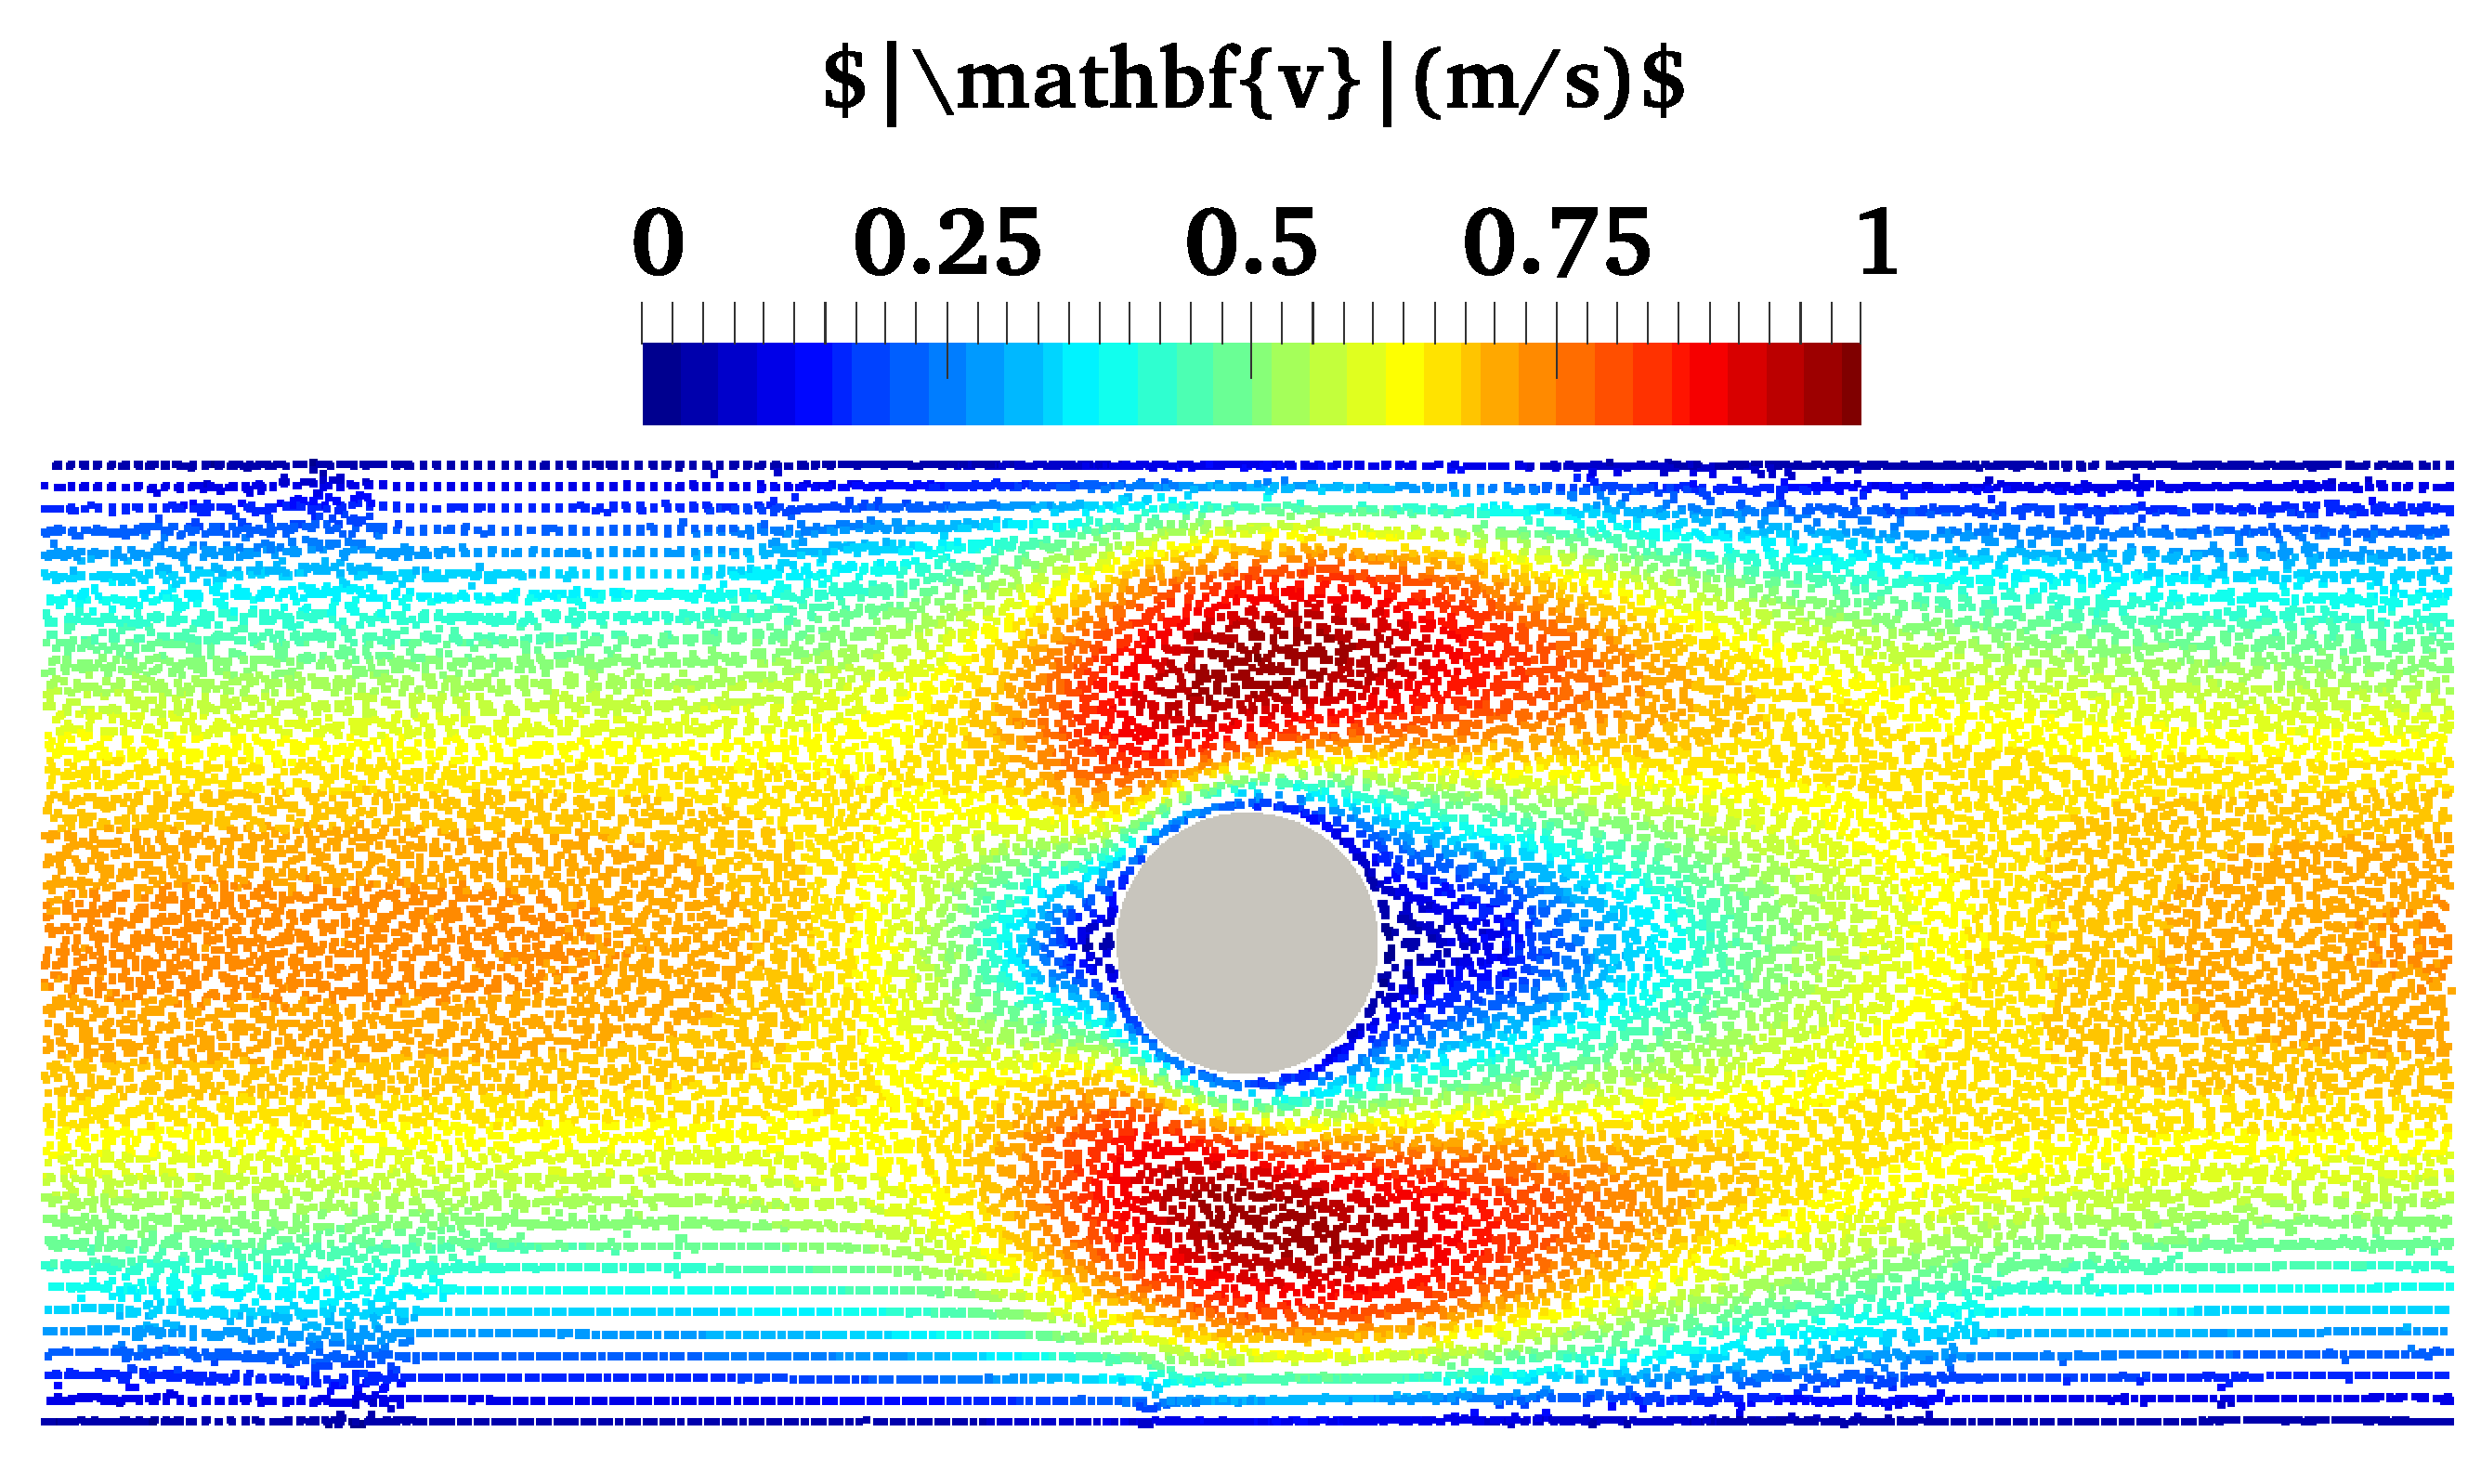
\includegraphics[width=1.0\textwidth]{images/SPH_Comparison/v_xsph.png}
	\end{subfigure}
	\begin{subfigure}{0.47\columnwidth}
		\centering
		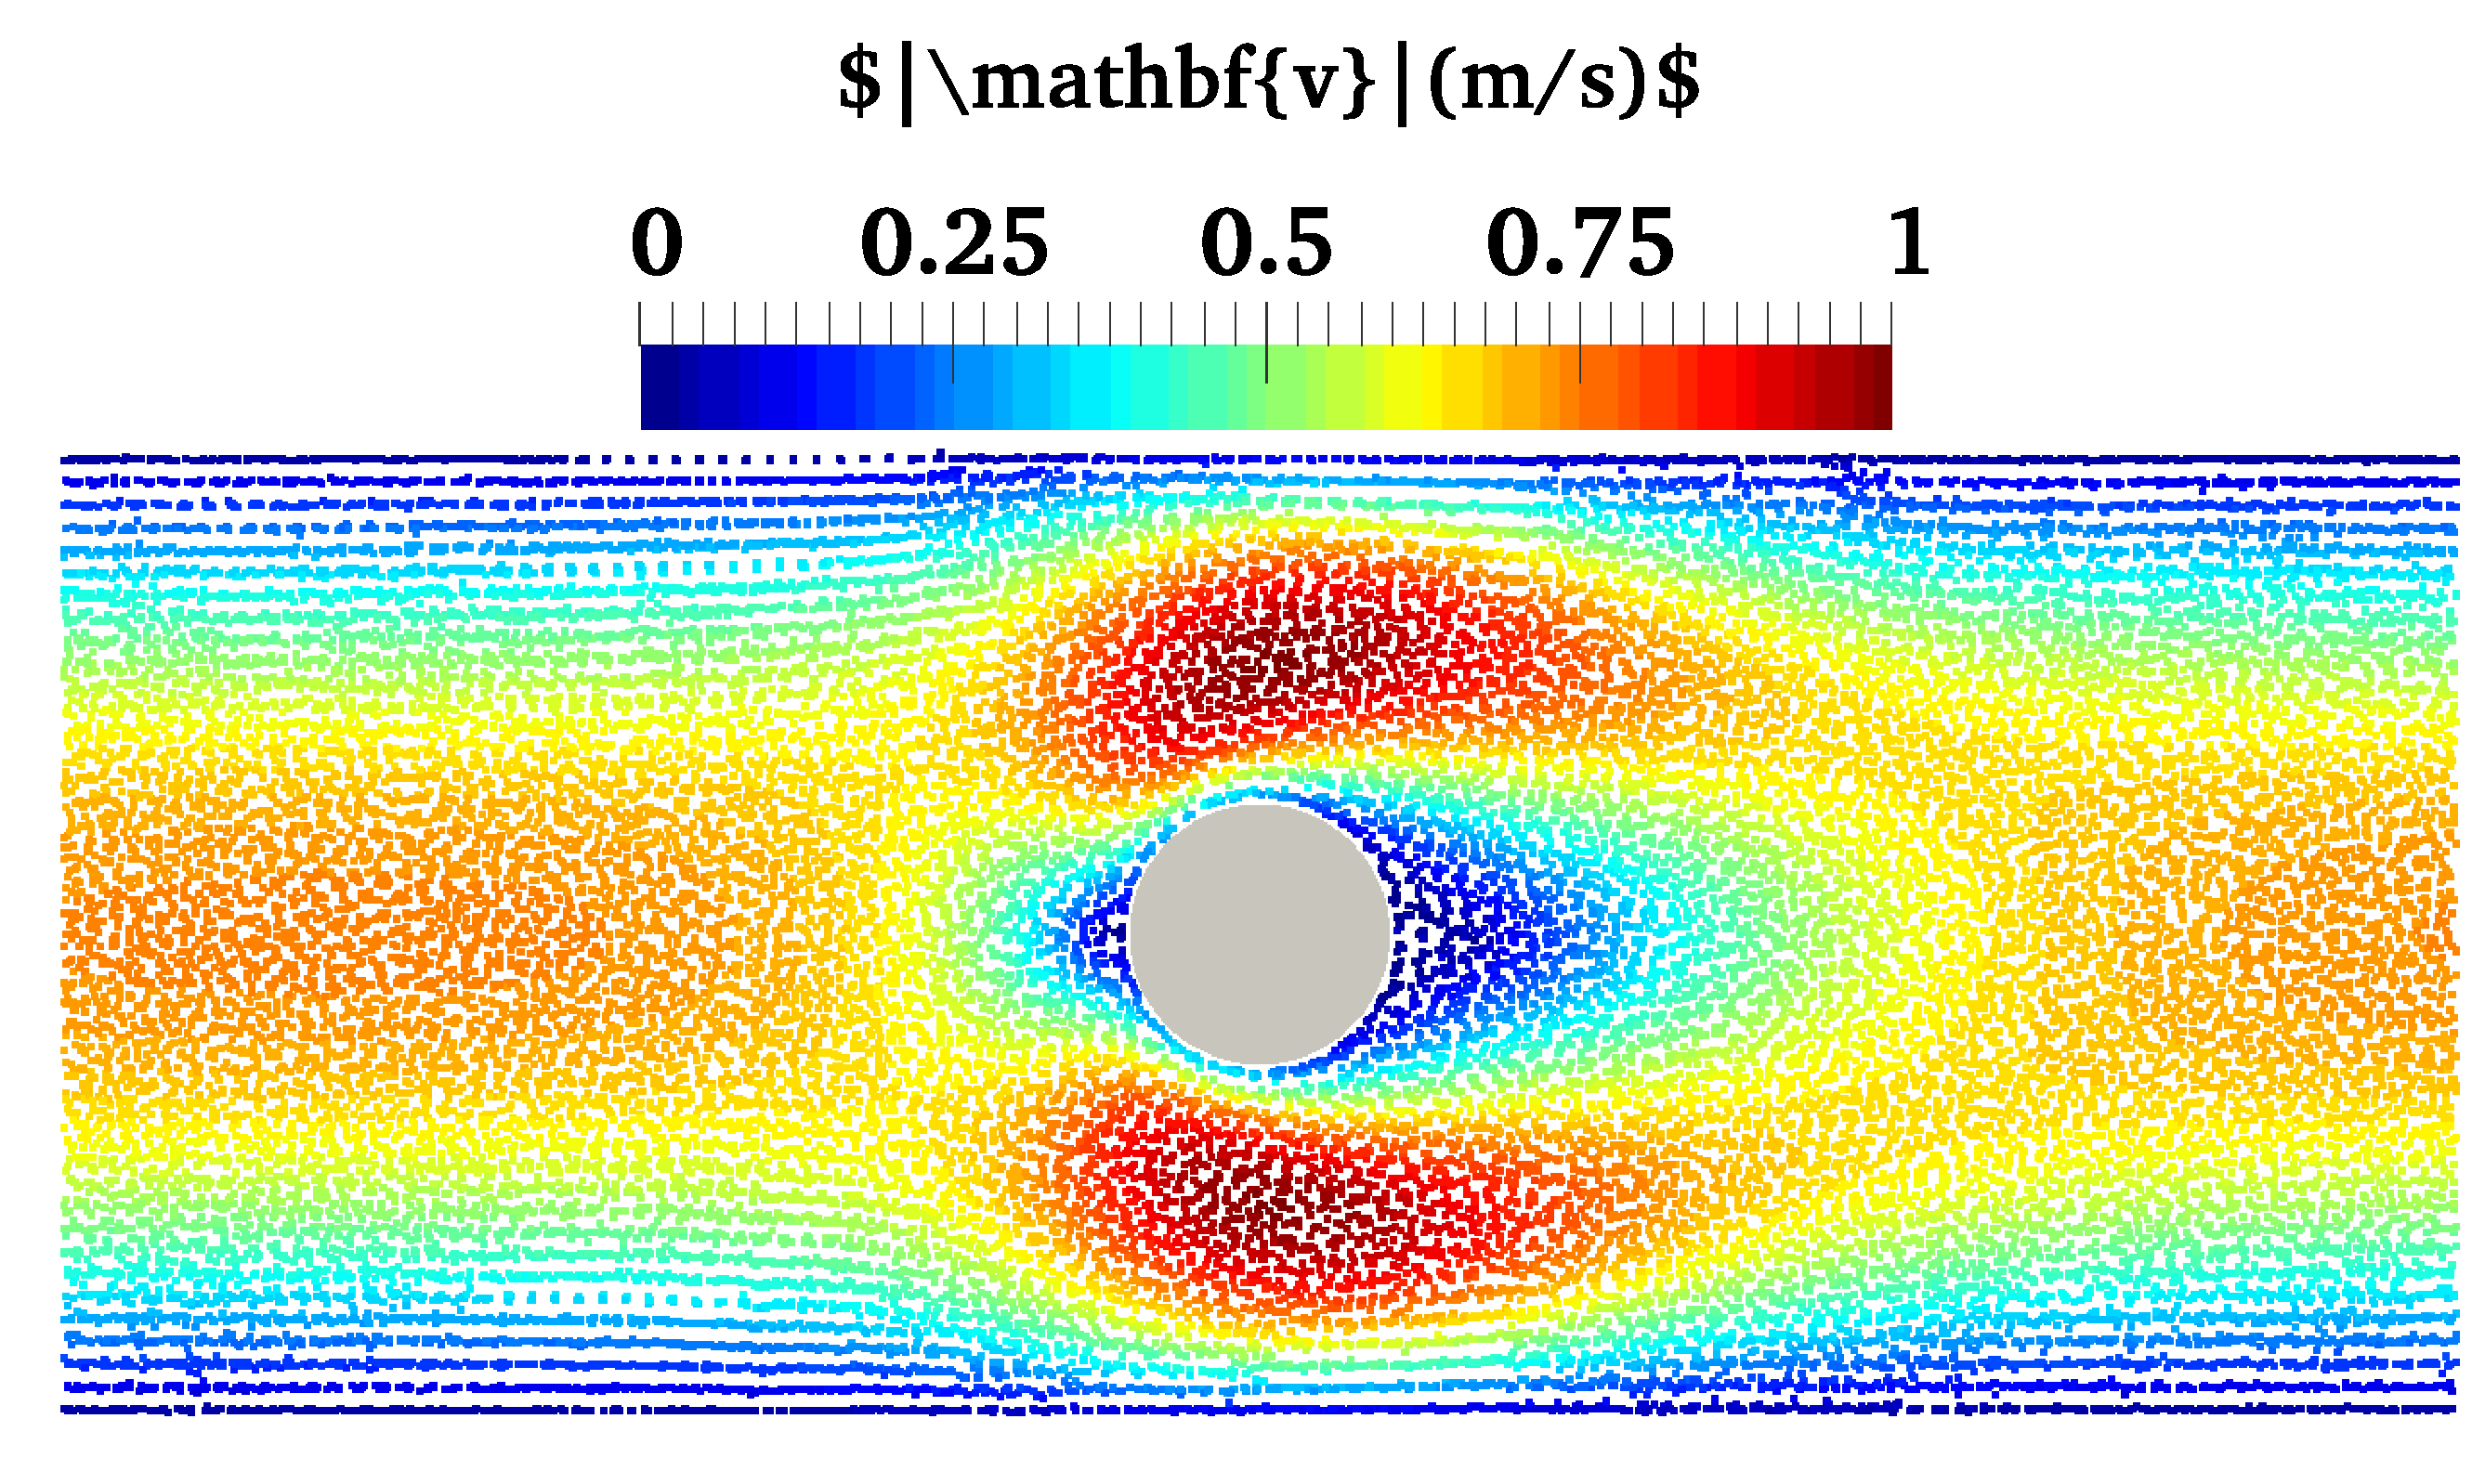
\includegraphics[width=1.0\textwidth]{images/SPH_Comparison/v_isph.png}
	\end{subfigure}
	\caption{Comparison of the steady-state velocity profiles predicted with WCSPH (left) and ISPH (right).}    \label{fig:FoCV}
\end{figure} 


We also note that there is no unique ISPH solution for pressure when solving the Poisson equation under pure Neumann boundary conditions -- in fact, the pressure solution is unique up to a constant. In other words, in the absence of Dirichlet boundary conditions, pressure is a relative quantity in the Navier-Stokes equations. Whereas the reference (\textit{minimum}) pressure for WCSPH is often set to zero, in ISPH, we choose the pressure solution with the \textit{average} value of zero.
Consequently, the difference between the legend of the plots in Fig.~\ref{fig:FoCP} has no real significance as long as the difference between the solutions is a constant offset that only indicates a reference pressure. Note that the choice of the reference pressure does not affect the gradient of the pressure, which is the quantity that comes into play in the Navier-Stokes equation.

\begin{figure}
	\centering    
	\begin{subfigure}{0.47\columnwidth}    
		\centering
		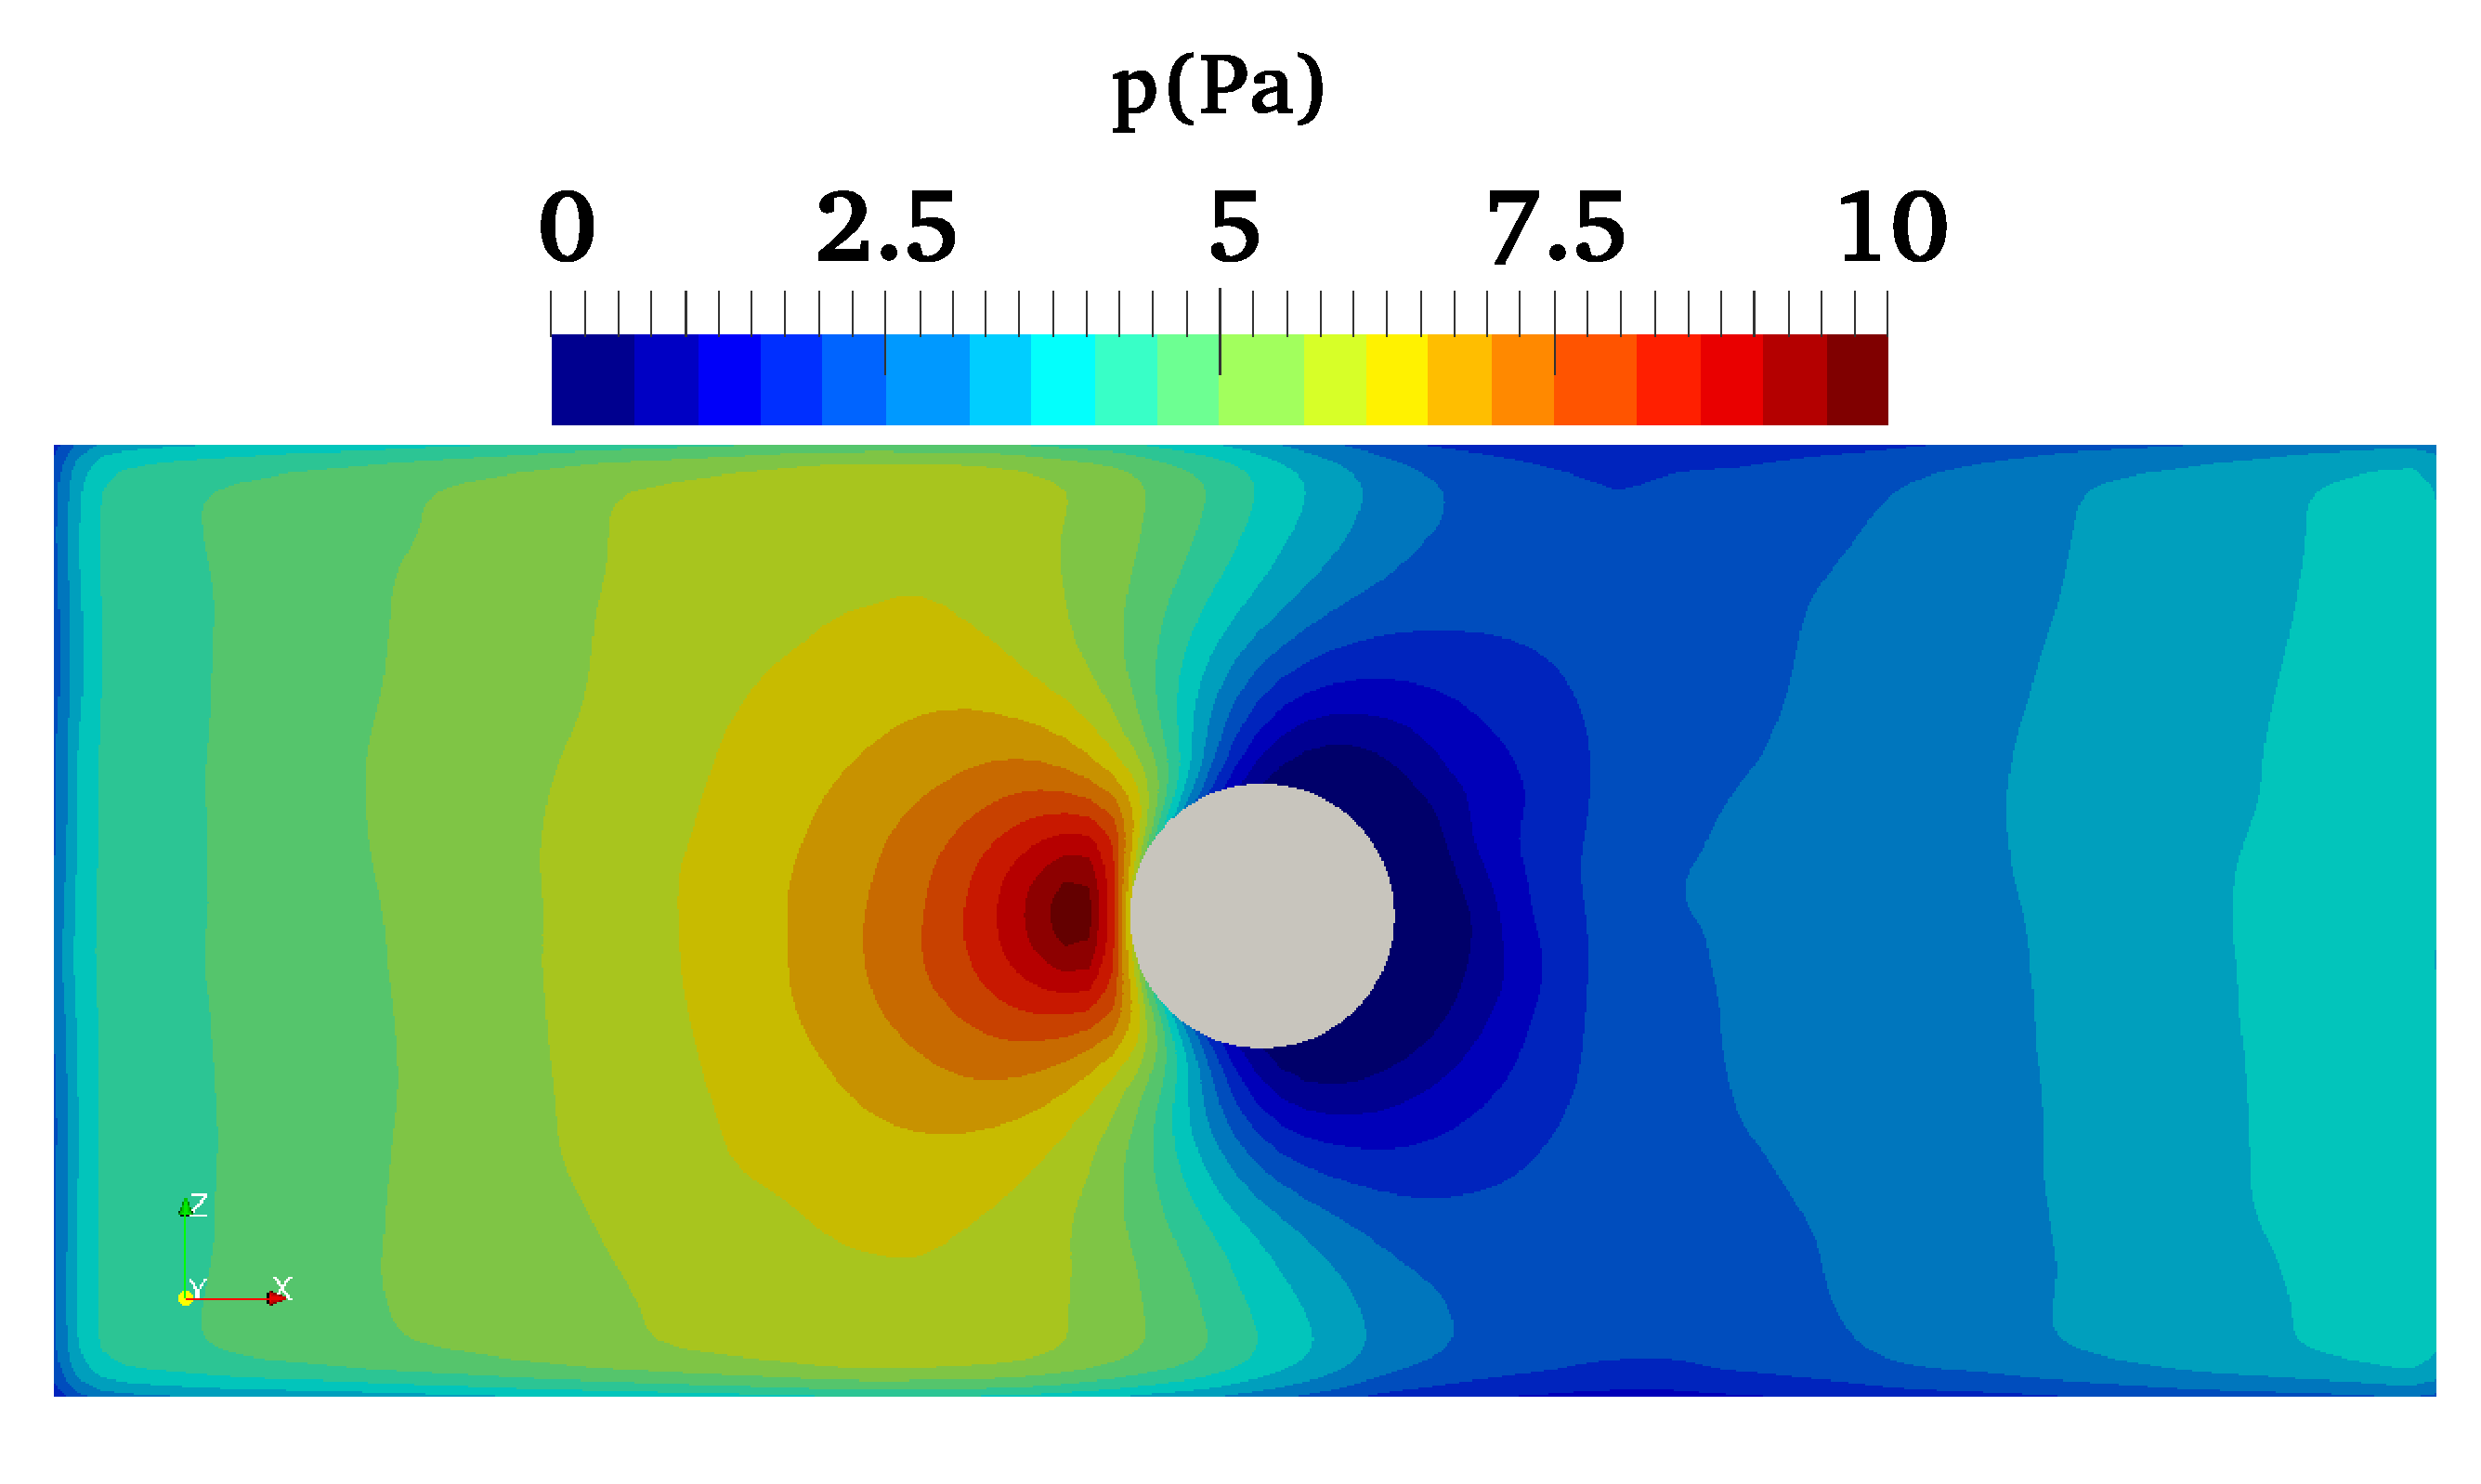
\includegraphics[width=1.0\textwidth]{images/SPH_Comparison/p_xsph.png}
	\end{subfigure}
	\begin{subfigure}{0.47\columnwidth}
		\centering
		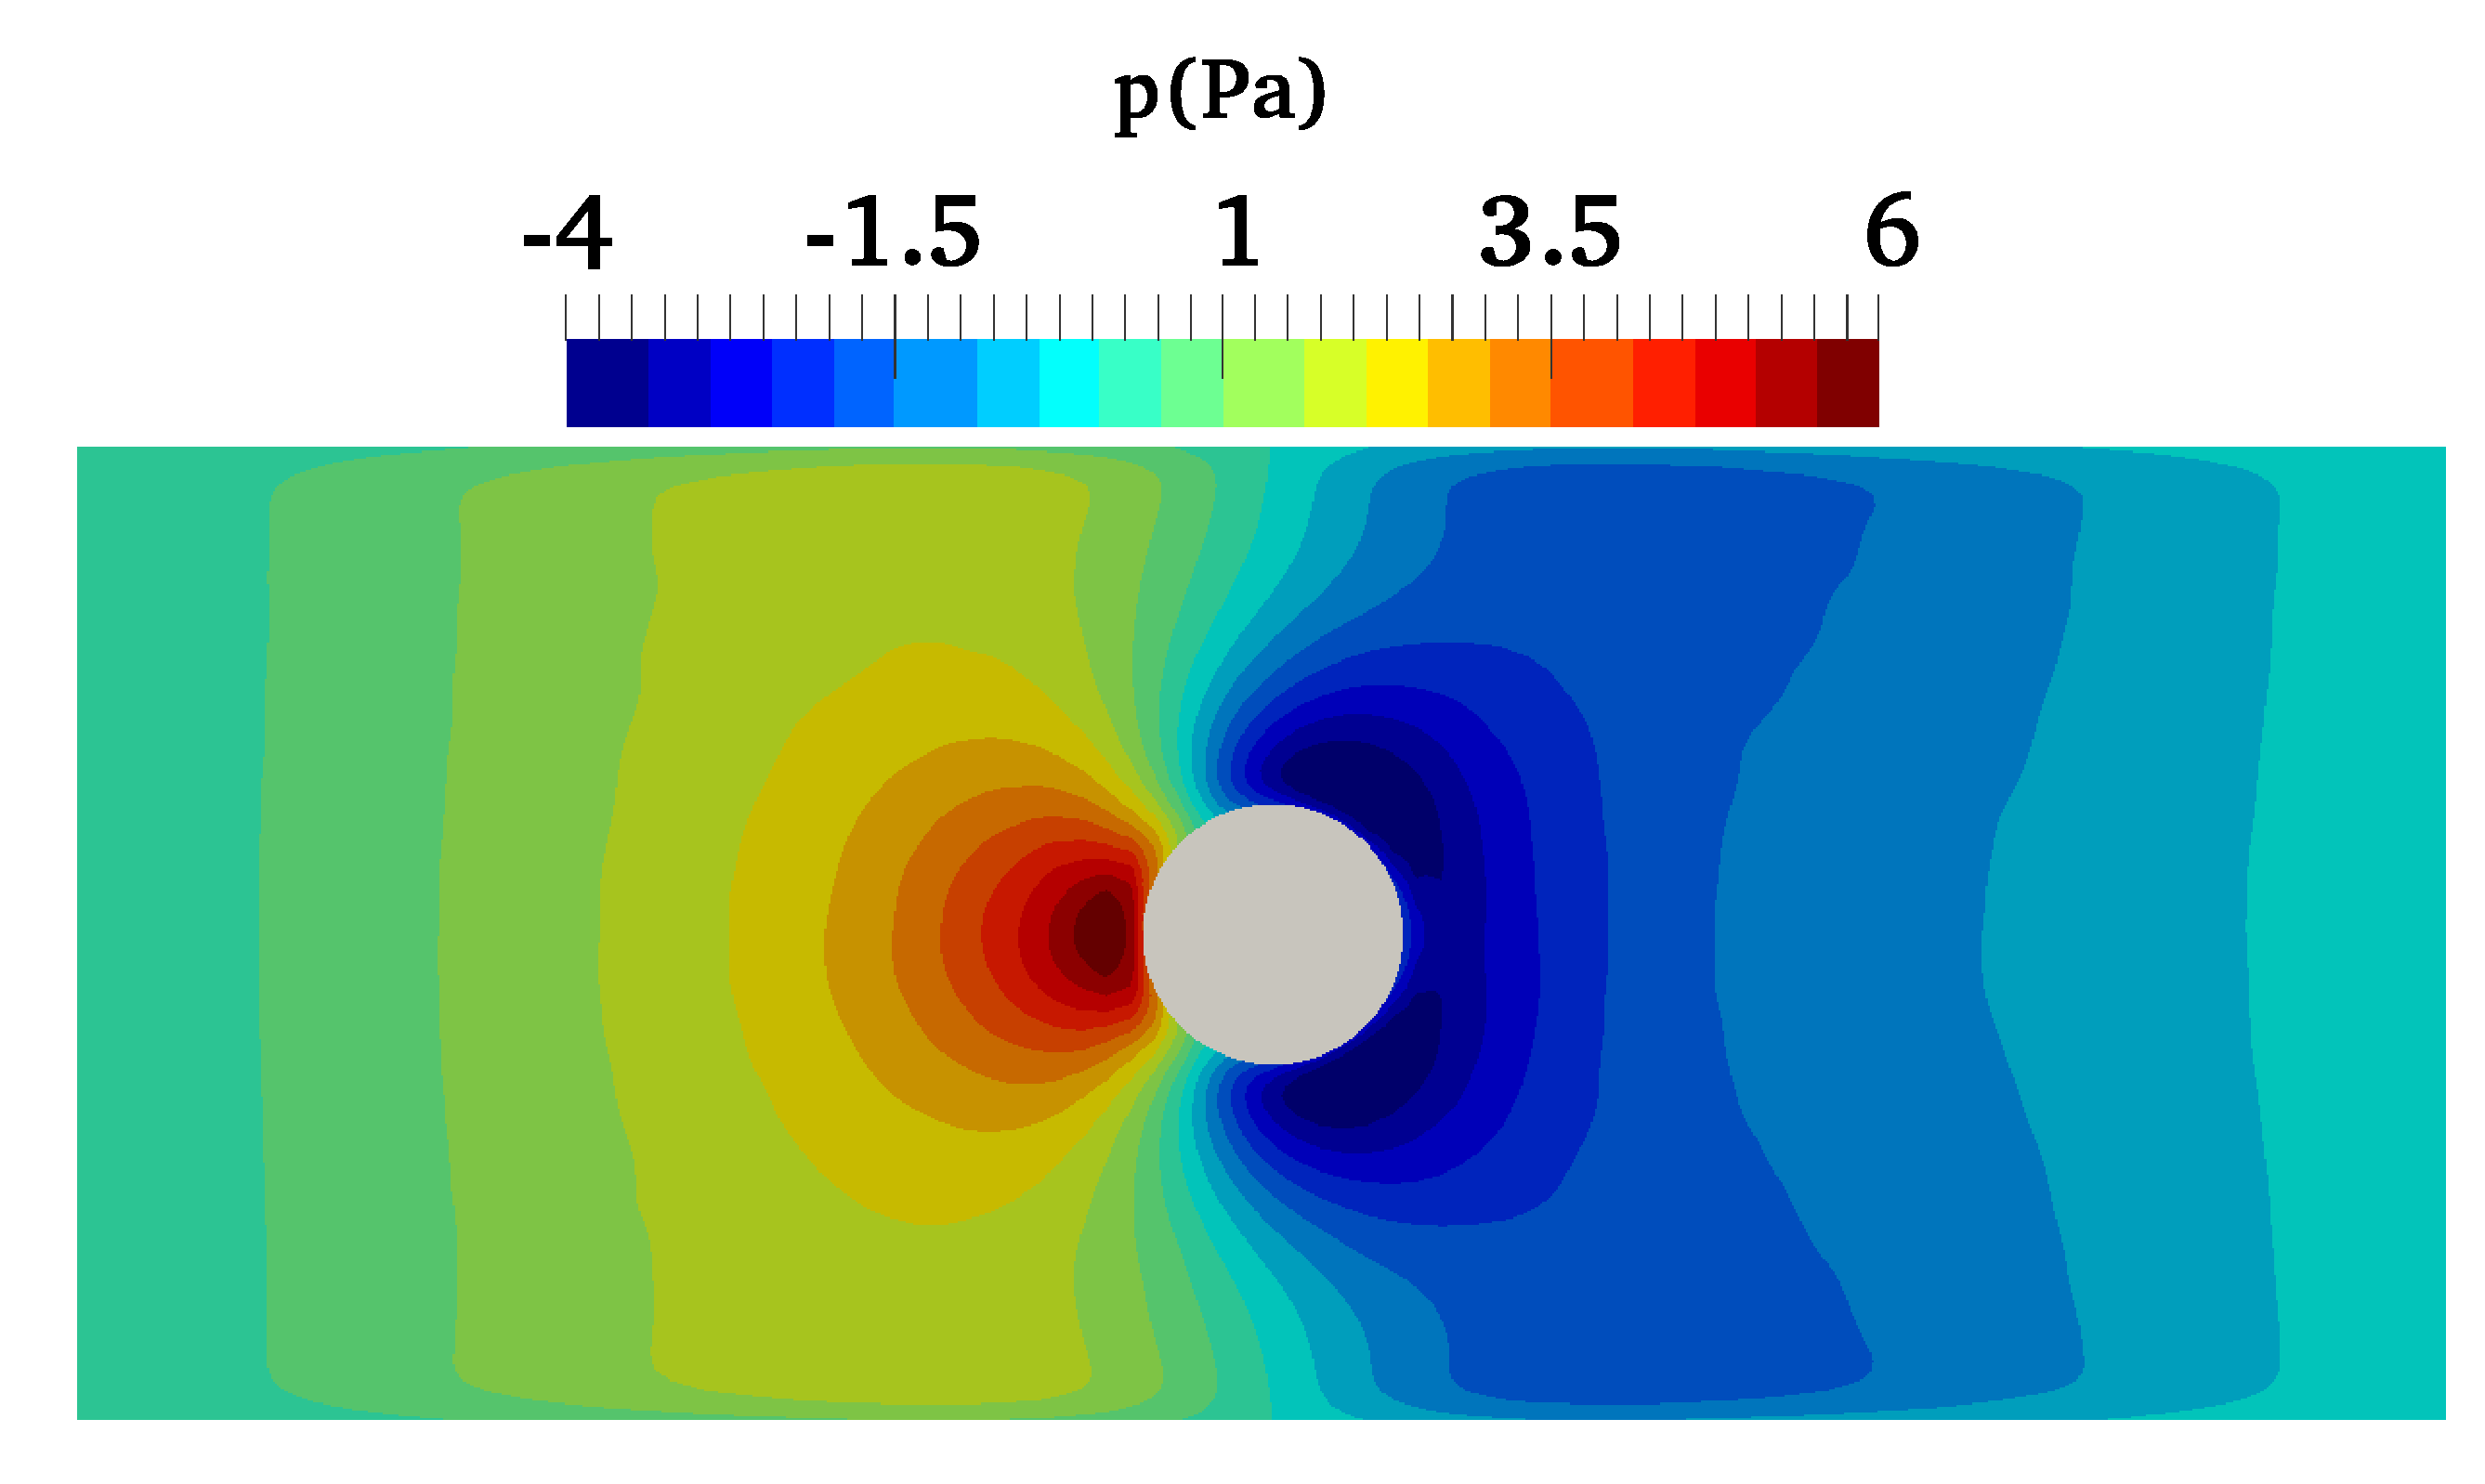
\includegraphics[width=1.0\textwidth]{images/SPH_Comparison/p_isph.png}
	\end{subfigure}
	\caption{Comparison of the steady-state pressure profiles predicted with  WCSPH (left) and ISPH (right).}    \label{fig:FoCP}
\end{figure} 
Herein, the expression used for the drag coefficient is $C_d=\frac{F_d}{0.5\rho\;A\; U^2}$, where $F_d$ is the drag force magnitude along the $x$ axis, $\rho=\rho_0$ and $U=1$\si{m/s} are the reference density and velocity, and $A$ is the frontal area of the cylinder. Comparing drag coefficient results is insightful since this exercise provides a macro-scale perspective that, while looking past micro-scale fluctuations, captures emergent behavior of practical relevance. As shown in Fig.~\ref{fig:FoC}, ISPH and WCSPH show different drag coefficients at the onset of the simulation yet the steady state solutions are in good agreement -- the relative error of the time-averaged drag coefficient over the last 2\si{s} of the simulations is $6.4$\%. We posit that two reasons contributing to these discrepancies are: ($i$) the different time-integration schemes used in the formulations (see Sections~\S\ref{sec:ISPH} and \S\ref{sec:WCSPH}), each with its own amount of numerical damping \cite{hairer2009odeBook}; and ($ii$) the vastly different treatment of the pressure by the two formulations.

\begin{figure}
	\vspace{-20pt}
	\begin{center}
		\includegraphics[width=0.5\textwidth]{images/SPH_Comparison/Figure_flow_around_cylinder.png}
	\end{center}
	\vspace{-10pt}
	\caption{Variation of the drag coefficient over time.}
	\label{fig:FoC}
\end{figure}


\subsection{Dam Break}
\label{subsec:damBreak}
Lagrangian methods such as SPH use the dam break benchmark test to assess the performance of fluid solvers in conjunction with a high transients, free-surface problem \cite{Martin1952,colagrossi2003numerical,hughes2010comparison,xu2016improved,miladHalfImplicit2018}. The fluid domain is a rectangular prism of size 2.0\si{m} $\times$ 0.5\si{m} $\times$ 1.0\si{m} consisting of \SI{64000} SPH particles that are placed on a regular lattice at $t=0$\si{s}. The reference density and viscosity are $\rho_0=1000$\si{kg/m^3} and $\mu=$\SI{0.001}{Pa.s}. The gravity $g=-9.8$\si{m/s^2} is applied in the  $z$ direction. The WCSPH, ISPH, and KCSPH results are compared from two perspectives: $(i)$ the fluid front position over time, and $(ii)$ the roll up and the second splash -- two characteristics highlighted in previous studies \cite{colagrossi2003numerical,Adami2012}. Figure~\ref{fig:db_front} shows the fluid front position as a function of time. While the KCSPH solution slightly over-estimate the front speed (no dissipation term is implemented in KCSPH), nearly identical front propagation is predicted by WCSPH and ISPH. 
\begin{figure}%[H]
	%    \vspace{-15pt}
	\begin{center}
		\includegraphics[width=0.5\textwidth]{images/SPH_Comparison/Figure_damBreak.png}
	\end{center}
	\vspace{-10pt}
	\caption{Comparison of water-front propagation between between KCSPH (top), WCSPH (middle), and ISPH (bottom).}
	\label{fig:db_front}
\end{figure}
With regard to the roll-up and second splash characteristics, all three methods predict well these two hallmark features of the dam break experiment, see Fig.~\ref{fig:db_charac}.
\begin{figure}[H]
	\centering    
	\begin{subfigure}{0.35\columnwidth}    
		\centering
		\includegraphics[width=1.0\textwidth]{images/SPH_Comparison/colorBar.png}
	\end{subfigure}
	
	\begin{subfigure}{0.4\columnwidth}    
		\centering
		\includegraphics[width=1.0\textwidth]{images/SPH_Comparison/cf_1.png}
	\end{subfigure}
	\begin{subfigure}{0.4\columnwidth}
		\centering
		\includegraphics[width=1.0\textwidth]{images/SPH_Comparison/cf_2.png}
	\end{subfigure}
	\begin{subfigure}{0.4\columnwidth}    
		\centering
		\includegraphics[width=1.0\textwidth]{images/SPH_Comparison/xsph_1.png}
	\end{subfigure}
	\begin{subfigure}{0.4\columnwidth}
		\centering
		\includegraphics[width=1.0\textwidth]{images/SPH_Comparison/xsph_2.png}
	\end{subfigure}
	\begin{subfigure}{0.4\columnwidth}    
		\centering
		\includegraphics[width=1.0\textwidth]{images/SPH_Comparison/isph_1.png}
	\end{subfigure}
	\begin{subfigure}{0.4\columnwidth}
		\centering
		\includegraphics[width=1.0\textwidth]{images/SPH_Comparison/isph_2.png}
	\end{subfigure}
	\caption{Comparison of the roll-up ($t=1.75$\si{s}, left) and the second splash ($t=2.05$\si{s}, right) characteristics between KCSPH (top), WCSPH (middle), and ISPH (bottom).}    
	\label{fig:db_charac}
\end{figure}

\subsection{Sloshing}
Sloshing probes the ability of a CFD solver to handle a free-surface problem that experiences lower frequency transients (when compared to the dam break). In this experiment a fluid container undergoes a forced vibration motion according to $X_0 = sin(2\pi f t)$, where $t$ is time, and $f$ and $X_0$ are the frequency and the amplitude of the vibration, respectively. The analytical solution of this problem under the inviscid flow assumption was discussed in \cite{Dodge2000} and involves a set of natural frequencies $\omega_n$ defined as
\[
\omega_n^2 =\left(2n-1\right) \pi \left(\frac{g}{w}\right) \text{tanh} \left[\left(2n-1\right) \pi \left(\frac{h}{w}\right)\right],
\]
where $n$ is the mode number, $g$ is the value of the gravitational acceleration, $w$ is the tank width; i.e., the tank dimension in the direction of oscillation, and $h$ is the height of the fluid at rest. The analytical amplitude $F_{x_0}$ of the net force exerted by the fluid on a sloshing tank in a forced vibration can then be expressed as 
\begin{equation*} 
\frac{F_{x_0}}{\Omega^2 X_0 m_l} = 1 + 8\frac{w}{h} \sum_{n=1}^{N} \frac{\text{tanh}\left[\left(2n-1\right) \pi h / w\right]}{\left(2n-1\right)^3 \pi ^3} \frac{\Omega ^2}{\omega_n^2 - \Omega^2} \;.
\end{equation*}
Above, $\Omega=2\pi f$ is the frequency of the oscillation and $m_l$ is the mass of the liquid. The exerted force on the container in the horizontal direction is expressed as  $F_x=F_{x_0} sin(2\pi f t)$.

We compare the ISPH, WCSPH, and KCSPH approximations with the analytical solution for the following problem: the dimension of the domain ($w \times b \times h$) is  1.2\si{m} $\times$ 0.4\si{m} $\times$ 1.7\si{m} and the  fluid density is $\rho_0=1000$\si{kg/m^3}. The gravity $g=-9.8$\si{m/s^2} is applied in the  $z$ direction. The numerical model is comprised of 98k SPH markers, which are placed on a uniform Cartesian lattice at $t=0$\si{s}. The frequency and amplitude of the vibration are set to be $f=0.75$\si{s^{-1}} and $X_0=0.1$\si{m}.  Figure~\ref{fig:Sloshing} reports the sloshing force exerted on the container over time. 
\begin{figure}[H]
	\begin{center}
		\includegraphics[width=0.7\textwidth]{images/SPH_Comparison/Figure_Sloshing.png}
	\end{center}
	\caption{Sloshing experiment: Comparison of fluid-structure interaction force along the axis of periodic motion.}
	\label{fig:Sloshing}
\end{figure}

Ignoring the initial transient period, all methods predict the dynamic interaction forces with reasonable accuracy. We attribute the initial discrepancy between the numerical and the analytical solutions to the fact that the simulation tank starts its motion from rest; hence the initial condition of the simulation is different from the analytical solution, the latter only reported in the steady-state regime. However, the initial transient motion is damped in approximately 1 \si{s}. As shown in Fig.~\ref{fig:Sloshing}, the steady-state solution of ISPH closely matches the analytical solution; the steady-state solution of the WCSPH slightly over-predicts, whereas the KCSPH solution under-predicts the analytical result.

\subsection{Discussion}\label{sec:discussion_SPHs}
This effort set out to gauge the agency of the SPH methodology, employed here in conjunction with three approaches to time stepping and incompressibility enforcement. WCSPH uses an equation of state for pressure along with explicit time stepping. ISPH falls back on a Poisson problem to enforce incompressibility Chorin-style time stepping. KCSPH enforces incompressibility via a kinematic constraint that asserts the constant value of the density while a half-implicit symplectic Euler integrator is used for time stepping. 

\vspace{3pt}

\noindent \textit{WCSPH, ISPH, KCSPH: Ease of implementation comments.} WCSPH and ISPH leveraged GPU computing through CUDA; KCSPH used multi-core parallel computing via OpenMP \cite{openMP}. The amount of effort required to implement these solvers in software was quite different. Implementing the WCSPH solver was easier than ISPH, which was easier than KCSPH. ISPH requires the solution of a sparse linear system on the GPU; such a solver is not readily available and herein, the implementation resorted to Krylov subspace iterative methods such as BICGSTAB and GMRES \cite{saad1989overview}. A memory-efficient solver requires sparse storage of the underlying systems (see Eqs.~\ref{eq:U_BC} and \ref{eq:p_BC}). Assembling and solving these sparse linear systems made the ISPH implementation nontrivial. KCSPH was more challenging to implement since it required at each integration step the solution of a constrained quadratic optimization problem, see \cite{hammadConstrFluid2018}. This optimization problem was posed in hundreds of thousands of variables -- as many as SPH particles used in the formulation and its solution was found using a Nesterov-type method \cite{hammadTOG2015}. 

\vspace{3pt}

\noindent \textit{WCSPH, ISPH, KCSPH: Solution robustness comments.}
KCSPH and ISPH  provide more robust (as in less finicky) solutions due to the coupling they establish between the field variables. Owing to the integration scheme used in ISPH, the velocity and pressure/density are coupled more tightly than in WCSPH, where pressure depends only on the density. Similarly in KCSPH, the pressures, which are a proxy of the Lagrange multipliers for the density kinematic constraints, are coupled with the velocity in a fully implicit sense. 

\vspace{3pt}

\noindent \textit{WCSPH, ISPH, KCSPH: Solution quality comments.} A simple answer to the question ``which method provides better quality results?'' is difficult to provide as multiple factors come into play in determining the quality of the solution, e.g., the particle resolution, the consistency vs. conservancy dichotomy, the decision to use or not particle shifting, the size of the time step, the nature of the problem solved, etc. This question is brought more into focus by stating that the interest is in obtaining results that are insightful without taxing tinkering with parameters, settings, etc. In general, ISPH turned out to be easier to set up and get good results with. It is robust (non-finicky) and for a given simulation time budget, it provides better quality results. One stumbling block is that ISPH requires a sparse linear solver. WCSPH, particularly for the non-consistent version, usually yields more noisy results -- this also came through in the flow-around-the-cylinder test. KCSPH shows potential, but it needs further investigation to improve the handling of viscosity and reduce execution speed as it requires the solution of a constrained convex optimization problem.

\vspace{3pt}

\noindent \textit{WCSPH, ISPH, KCSPH: Time to solution comments.}
While an efficiency comparison of WCSPH, ISPH, and KCSPH falls outside the scope of this contribution owing to the sheer scope of such an undertaking, we considered insightful to provide timing results to understand, insofar as order of magnitude is concerned, how long an SPH simulation would take. The problem considered was the dam break simulation of \S\ref{subsec:damBreak}. There was no attempt to optimize the WCSPH, ISPH, and KCSPH implementations, which were made in Chrono. Therein, WCSPH and ISPH rely on GPU computing; KCSPH draws on OpenMP. %We find this {\textit{qualitative}} information useful to understand, as order of magnitude, simulation times associated with this benchmark SPH problem. 
Table~\ref{tab:speed} shows {\textit{qualitative}} information regarding the first second of simulation of the dam break problem. All 3D solvers used \SI{215000} SPH markers. WCSPH takes smaller step sizes due to the explicit time stepping. However, its effort per time step is both step-size independent and cheaper than for ISPH or KCSPH. For the latter two, given the iterative nature of the solution process, higher computational costs are incurred for larger step sizes. Note that even for the same integration time step, the amount of time required to converge at different points in the ISPH/KCSPH simulation might be different owing to the difference in the number of iterations that the underlying linear system/optimization solvers require to converge. 
\begin{table}\centering
	\begin{tabular}{cccc}
		\toprule
		
		method & $\Delta t$(\si{s}) &  simulation time (\si{s}) & average time per step (\si{s})\\
		\midrule
		
		WCSPH & $10^{-4}$ & 1646 & 0.17 \\
		WCSPH & $2.5\times 10^{-4}$ & 682 & 0.17 \\
		ISPH & $10^{-3}$ & 1692 & 1.69 \\
		ISPH & $5\times 10^{-3}$ & 369 & 1.84 \\
		
		KCSPH & $10^{-3}$ & 1523 & 1.52 \\
		KCSPH & $5\times 10^{-3}$ & 531 & 2.65 \\
		\bottomrule
	\end{tabular}
	\caption{Dam break, qualitative information: solver execution times for the first second of the simulation.}
\end{table}\label{tab:speed}

\vspace{3pt}

\noindent \textit{WCSPH, ISPH, KCSPH: Use case recommendations.}
WCSPH is the method of choice for many single-phase and free-surface CFD problems such as the dam break and Poiseuille flow. ISPH was found to be a better choice when more complex physics, e.g., vortex shedding, boundary layer separation, etc., are present. This is the case for problems like flow around cylinder and the flow over backward facing step at higher Reynolds numbers ($Re\approx 10^2$--$10^3$). ISPH is also the solver of choice for FSI problems with relatively simple boundary geometries. KCSPH leverages multi-body dynamics approaches, which opens the door to monolithic frameworks for more involved FSI problems, e.g., fording scenarios with complex vehicle models (wheeled, tracked) \cite{hammadConstrFluid2018}. Indeed, imposing ISPH or WCSPH boundary conditions on a complex mesh, e.g., a vehicle, requires a uniformly generated point cloud, whereas KCSPH does not have this restriction and is more flexible in terms of boundary condition enforcement. 

%\vspace{3pt}
%
%\noindent \textit{WCSPH, ISPH, KCSPH: Connections to other physics.} The inspiration for the KCSPH method used in this study is a granular dynamics solution approach. Indeed, WCSPH has a granular dynamics twin in the discrete element method (DEM) \cite{cundall79}. However, there is a second class of granular dynamics methods that belongs to the family of ``contact dynamics'' or differential variational inequality approaches, in which the non-penetration condition is enforced by kinematic constraints, see, for instance \cite{negrutSerbanTasoraJCND2017}. The ``contact dynamics'' twin in fluid dynamics would be one that explicitly states that $\rho(t) = \rho_0$; i.e., KCSPH. Continuing this granular dynamics--fluid dynamics parallel, the analog of the contact force in granular dynamics is the pressure in fluid dynamics; likewise, the friction force at the contact between two grains is the twin of the shear force in fluid dynamics. Another salient point in this analogy is that the pressure in ISPH is the analog of the Lagrange multiplier that enforces the $\rho(t) = \rho_0$ in KCSPH, made clear in this contribution by casting the SPH spatial discretization in a matrix-vector form. This is unsurprising given that in an incompressible, Newtonian fluid model the pressure is devoid of a thermodynamic trait and instead becomes a mechanical attribute of the flow. For Newtonian fluids though, the analogy ends here -- while for a Newtonian fluid the shear force only depends on velocity, in granular dynamics the friction force is tied to the contact (normal) force through a yield condition that caps the former at a value equal to the normal force scaled by $\mu$, the friction coefficient: $f_f \leq \mu f_n$.





\section{IISPH Method}\label{sec:IISPH_Val}
\subsection{Incompressibility Test}
\label{subsec:incompressibilityTest}
In this test we monitor the value of the density over time for a fluid stored in a container. A rectangular container with dimensions \SI{1.1}{m} (L) $\times$ \SI{1.1}{m} (W) $\times$ \SI{1.2}{m} (H) is initialized with fluid particles. The particles are free to move inside the container under the influence of viscous and gravitational forces. We seek to understand how successful the IISPH solution implemented is in enforcing the incompressibility condition. The reference WCSPH solution is provided by the open-source software DualSPHysics  \cite{crespo2015dualsphysics}. In DualSPHysics, the maximum CFL value was set to \num{0.1}, i.e. $C_{max}=0.1$, and the speed of sound $c_s$ was varied to obtain different levels of compressibility. Other settings were carried over from the dam break tutorial provided with DualSphysics \cite{crespo2015dualsphysics}. Both solvers used approximately \num{56000} SPH particles to include a \num{32}$\times$\num{32}$\times$\num{35} distribution of particles plus additional BCE particles. 

Figure~\ref{fig:Compressibility_Comparison} confirms that increasing $c_s$ in WCSPH leads to smaller density errors. However, the larger $c_s$, the stiffer the numerical problem, which translates into smaller integration step size. Thus, at one end of the spectrum, WCSPH uses small yet computationally inexpensive time steps. At the other end of the spectrum, IISPH allows for large albeit more computationally costly time steps. Against this backdrop, Fig.~\ref{fig:Compressibility_Comparison} answers the following question: what value of $c_s$ and $\Delta t_{WCSPH}$ should be used for DualSPHysics so that the quality of the solutions produced by IISPH and WCSPH are comparable? As shown in Fig.~\ref{fig:Compressibility_Comparison}, an approximately $100$-fold larger time step can be adopted by the IISPH method for the same level of compression. The vertical axis in the figure shows the relative error at every time step, which is defined, for the time step $(l)$ as
\[
\% \mbox{ error}^{(l)}  \equiv (\frac{1}{\rho_0 \nFluid } \sum_{i=1}^{\nFluid} \rho_i^{(l)} -1) \times 100 \; ,
\]
\noindent where $N_F$ is the number of SPH particles; in Fig.~\ref{fig:Compressibility_Comparison}, ``tol'' stands for the tolerance used in the linear solver. Recall though that the larger IISPH step size comes at the cost of solving a linear system of equations at each time step.
%\input{images/Compressibility.tex}
\begin{figure}[H]
	\begin{center}
		\includegraphics[width=0.9\textwidth]{images/IISPH/tikz/Compressibility.png}
	\end{center}
	\caption{IISPH vs. WCSPH (DualSPHysics \cite{crespo2015dualsphysics}) comparison based on the relative drift in the incompressibility.}
	\label{fig:Compressibility_Comparison}
\end{figure}

%\subsection{Dam Break}
%The dam break is often used to assess the performance of fluid solvers for free-surface simulation \cite{Adami2012,Martin1952,colagrossi2003numerical,hughes2010comparison}. The fluid behind the dam fits in a cube of $1$ \si{m} (height), $1$ \si{m} (width) and $0.5$ \si{m} (depth). The reference density is $\rho=1$ \si{kg/m^3}. At  $t=0$ \si{s}, the SPH particles are placed on a uniform Cartesian lattice. The gravity $g=1$ \si{m/s^2} is applied in the negative $y$. The approximate Reynolds number is $Re \approx 400$ \cite{Adami2012}. Upon conducting a particle resolution study with SPH characteristic lengths of $0.05$, $0.025$, $0.0125$ \si{m}, which resulted in \num{61000}, \num{245000}, and \num{1070000} SPH particles respectively, we observed the results are practically size-independent beyond the intermediate resolution. Good agreement between numerical results and experimental data \cite{Martin1952} is observed for $t<2$, see Fig.~\ref{fig:waterFront}. The simulation results slightly over-predict the experimental data after $t=2$, which is a trend reported in previous studies \cite{Adami2012,asai2012stabilized}. This discrepancy has been attributed to uncertainties resulting from several factors including lack of surface-tension model and the numerical viscosity formulation \cite{Adami2012}.
%\tikzsetnextfilename{waterFront}
\tikzset{external/export next=false}
\begin{figure}[H]
	\centering
	\begin{tikzpicture}
		\begin{axis}[
			width=0.6\columnwidth,
			%height=0.6\textwidth,
			xlabel = $t(gH)^{-1/2}$,
			ylabel = $x_{front}/H$,
			xmin=0, xmax=3.2,
			ymin=0, ymax=6,
			xtick={0,0.5,...,3},
			ytick={0,1,...,6},
			minor y tick num={1},
			minor x tick num={1},
			y tick label style={
				/pgf/number format/fixed,
				/pgf/number format/fixed zerofill,
				/pgf/number format/precision=1},
			axis x line=middle,
			axis y line=middle,			
			grid=both,
			grid style={dotted},
			%legend cell align = left,
			x tick label style={/pgf/number format/fixed},
			%no marks,
			]
			\addplot[black,very thick,,only marks, mark=o]
			table[
			x index={0},
			y index={1}, 
			]{images/Figs/Front_Pos_damBreak.txt};
			
			\addplot[black,very thick]
			table[
			x expr=\thisrowno{0},
			y expr=\thisrowno{1}+2.75, %This is the offset of the corner of the dam
			]{images/Analysis_DamBreak.txt};
			\legend{\small Martin and Moyce \cite{Martin1952},  \small Present Study}
			
			
\texttt{}%			\addplot[black,very thick,dashed,domain=0:4, samples=20]
%			{1.8*(x-0.45)};
%			\legend{\small Martin and Moyce \cite{Martin1952},  \small Present Study}
%					
		\end{axis}
	\end{tikzpicture}
%	\caption{Lift coefficient}
		\caption{Comparison of water-front propagation between IISPH  and experimental results of Martin and Moyce \cite{Martin1952,Shao2003}.}
			\label{fig:waterFront}
\end{figure}
%%\begin{figure}[H]
%%	\begin{center}
%%		\includegraphics[width=0.65\textwidth]{tikz/DamBreak.pdf}
%%	\end{center}
%%		\caption{Comparison of water-front propagation between IISPH  and experimental results of Martin and Moyce \cite{Martin1952,Shao2003}.}
%%\label{fig:waterFront}
%%\end{figure}
%
%Next, we compare our results with the classical dam break simulation discussed in \cite{colagrossi2003numerical}. To this end, the fluid height was $1$ \si{m}, width was $2$ \si{m}, and the size of the domain in which the fluid moved was $5.36$ \si{m}. The highlights of the dam break benchmark; i.e.,  the roll-up and the second splash \cite{colagrossi2003numerical,Adami2012}, can be captured by the current formulation as shown in Fig. \ref{fig:dambreak}. The simulation ran for 12 \si{s} and showed no instability issues. An animation of this simulation is available at \cite{sbelWebsiteAnimations} as movie \#139.
%
%\begin{figure}[t]
%	\vspace{-40pt}
%	\centering
%	\begin{subfigure}{0.3\columnwidth}	
%		\centering
%		\includegraphics[width=1.0\textwidth]{images/IISPH/Color_Dambreak.png}
%	\end{subfigure}
%	
%	\begin{subfigure}{0.4\columnwidth}	
%		\centering
%		\includegraphics[width=1.0\textwidth]{images/IISPH/low2_0020.png}
%	\end{subfigure}
%	\begin{subfigure}{0.4\columnwidth}	
%		\centering
%		\includegraphics[width=1.0\textwidth]{images/IISPH/high_0020.png}
%	\end{subfigure}
%	
%	\begin{subfigure}{0.4\columnwidth}	
%		\centering
%		\includegraphics[width=1.0\textwidth]{images/IISPH/low2_0040.png}
%	\end{subfigure}
%	\begin{subfigure}{0.4\columnwidth}	
%		\centering
%		\includegraphics[width=1.0\textwidth]{images/IISPH/high_0040.png}
%	\end{subfigure}
%	\begin{subfigure}{0.4\columnwidth}	
%		\centering
%		\includegraphics[width=1.0\textwidth]{images/IISPH/low2_0075.png}
%	\end{subfigure}
%	\begin{subfigure}{0.4\columnwidth}	
%		\centering
%		\includegraphics[width=1.0\textwidth]{images/IISPH/high_0075.png}
%	\end{subfigure}
%	
%	\begin{subfigure}{0.4\columnwidth}	
%		\centering
%		\includegraphics[width=1.0\textwidth]{images/IISPH/low2_0090.png}
%	\end{subfigure}
%	\begin{subfigure}{0.4\columnwidth}	
%		\centering
%		\includegraphics[width=1.0\textwidth]{images/IISPH/high_0090.png}
%	\end{subfigure}
%	
%	\begin{subfigure}{0.4\columnwidth}	
%		\centering
%		\includegraphics[width=1.0\textwidth]{images/IISPH/low2_0100.png}
%	\end{subfigure}
%	\begin{subfigure}{0.4\columnwidth}	
%		\centering
%		\includegraphics[width=1.0\textwidth]{images/IISPH/high_0100.png}
%	\end{subfigure}
%	
%	\begin{subfigure}{0.4\columnwidth}	
%		\centering
%		\includegraphics[width=1.0\textwidth]{images/IISPH/low2_0110.png}
%		\caption{h=0.025\si{m}, \num{215000} SPH particles.}	
%	\end{subfigure}
%	\begin{subfigure}{0.4\columnwidth}	
%		\centering
%		
%		\includegraphics[width=1.0\textwidth]{images/IISPH/high_0110.png}
%		\caption{h=0.0125\si{m}, \num{928000} SPH particles.}	
%	\end{subfigure}
%	
%	%\begin{subfigure}{0.4\columnwidth}	
%	%	\centering
%	%	\includegraphics[width=1.0\textwidth]{images/low.0120.png}
%	%\end{subfigure}
%	%\begin{subfigure}{0.4\columnwidth}	
%	%	\centering
%	%	\includegraphics[width=1.0\textwidth]{images/high_0120.png}
%	%\end{subfigure}
%	\caption{Dam-break simulation at t =0.4, 0.8, 1.5, 1.8, 2.0, and 2.2 for two different resolutions.}	\label{fig:dambreak}
%\end{figure} 
%\FloatBarrier

\subsection{Flow Around a Cylinder}
The IISPH results have been compared with results of a finite volume method simulation run in OpenFOAM \cite{weller1998tensorial}. In this test, a cylinder of radius 0.05~\si{m} was positioned at the center of a rectangular domain of height 0.4~\si{m} and length 1.0~\si{m}. No-slip boundary conditions were applied to the top and bottom walls while periodic (cyclic) conditions were maintained at the left (inlet) and right (outlet) patches. A constant body force of $f_b$=0.02~\si{m/s^2} was applied in order to balance the viscous forces. The study was conducted at $Re={\rho V_{max} D}/{\mu}\approx 30 $.

In order to model the problem in OpenFOAM, a block-structured mesh was created in $blockMesh$. In the neighborhood of the cylinder, the size of the mesh-element was chosen equal to the SPH characteristic length $h$ (see Eq.~\ref{eq:kernelExample}). The OpenFOAM $pimpleFoam$ solver was employed to reach the steady state solution and $fvOptions$ was used to apply a body force (source term) to the momentum equations. The simulation was run for 10 \si{s} to reach steady state. A dynamic time-step was adopted to maintain ${V_{max}\Delta t}/{\Delta x} =0.2$. Other settings were kept similar to the configuration of the $elipsekkLOmega$ OpenFOAM test, which is made available as a tutorial in OpenFOAM's distribution.

Figure~\ref{fig:FoC_IISPH} illustrates the velocity fields of the Lagrangian method (IISPH) and the Eulerian method (OpenFOAM). Figure~\ref{fig:FOC_profiles} contains a plot of the velocity magnitude vs. vertical position $y$ at two sections of the domain: $x$=0.0 \si{m} (middle) and at $x$=0.5 \si{m} (outlet). The finite volume method turned out to be more apt at enforcing no-slip boundary conditions, which comes as no surprise given the meshless nature of SPH.

\begin{figure}[H]
	\centering
	\begin{subfigure}{0.4\columnwidth}	
		\centering
		\includegraphics[width=0.8\textwidth]{images/IISPH/ColorBar.png}
	\end{subfigure}
	
	\begin{subfigure}{0.64\columnwidth}	
		\centering
		\includegraphics[width=0.8\textwidth]{images/IISPH/focSPH.png}
	\end{subfigure}
	
	\begin{subfigure}{0.6\columnwidth}
		\centering
		\includegraphics[width=0.8\textwidth]{images/IISPH/focFV.png}
	\end{subfigure}
	\caption{Comparison of the velocity profiles predicted with IISPH method (top) and OpenFOAM (bottom). The SPH data was mapped to a grid for the sake of comparison.}	\label{fig:FoC_IISPH}
\end{figure} 

%\input{images/FOC.tex}
\begin{figure}[H]
	\begin{center}
		\includegraphics[width=0.6\textwidth]{images/IISPH/tikz/FOC.png}
	\end{center}
	\caption{Comparison of the velocity profiles obtained with IISPH and OpenFOAM's finite volume method at two sections of the domain: center, $x$=0 \si{m}, and outlet, $x$=0.5 \si{m}.}
	\label{fig:FOC_profiles}
\end{figure}

\subsection{Elastic Gate Experiment}
The elastic gate test, used in \cite{Antoci2007,yang2012,jahanbakhsh2015}, is considered here in order to validate the fluid/deformable-solid coupling. In this experiment, water is stored in a cubic container that has three rigid sides and a fourth side partially made up of a rectangular elastic rubber gate, see the $t=0$ \si{s} snapshot shown in Fig.~\ref{fig:Elastic_Gate_Schematic}. Due to the hydrostatic pressure of the water, the elastic gate gradually deflects and the water starts pouring through the gate. The position of the tip of the gate was measured in the experiment reported in \cite{Antoci2007}. Our simulation was carried out with \num{79000} SPH markers. The results shown in Fig.~\ref{fig:FSI_Validation} are in good agreement with the numerical and experimental results reported in \cite{Antoci2007}. 

%\tikzsetnextfilename{Elastic_Gate_Schematic}
%\tikzset{external/export next=false}
\begin{figure}
	\centering
	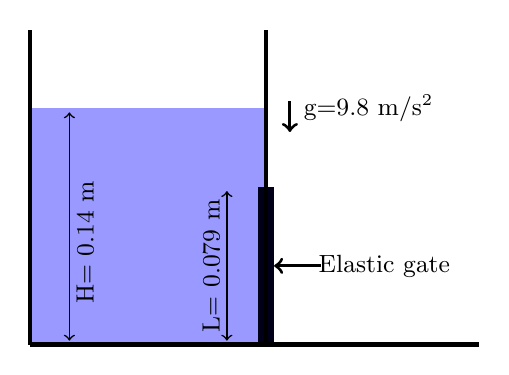
\begin{tikzpicture}
			\fill[blue!40!white] (-3,0) rectangle (0,3);
			\fill[blue!10!black] (-0.1,0) rectangle (0.1,2);
			\draw[<-,line width=0.4mm] (0.1,1) -- (0.7,1);
			\draw (1.5,1) node []{\small Elastic gate };
			
				%Ground
				\draw  (-3,0) -- (2.7,0) [line width=0.6mm];
				\draw  (-3,0) -- (-3,4) [line width=0.5mm];
				\draw  (0,0) -- (0,4) [line width=0.5mm];
		
		\draw (1.3,3) node []{\small g=9.8 \si{m/s^2}};
		\draw[<-,line width=0.4mm] (0.3,2.7) -- (0.3,3.1);
				
		\draw[<->,line width=0.2mm] (-0.5,0.05) -- (-0.5,1.95) ;
		\draw (-0.7,1) node [rotate=90] {\small L= 0.079 \si{m}};
		
		\draw[<->,line width=0.2mm] (-2.5,0.05) -- (-2.5,2.95) ;
		\draw (-2.3,1.3) node [rotate=90] {\small H= 0.14 \si{m}};
		
%		\draw[<->,line width=0.2mm] (-2.95,3.2) -- (-0.05,3.2) ;
%		\draw (-1.5,3.4) node [] {\small B= 0.1 \si{m}};
%
%		\draw (-2.1,6) node [] {\small Water properties: };
%		\draw (-0.9,5.6) node [] {\small $\rho$=1000 \si{kg/m^3} , $\mu $=0.0001 \si{Pa.s} };
%		\draw (-1.7,5) node [] {\small Elastic gate properties:};
%		\draw (-0.2,4.6) node [] {\small $\rho_s$=1100 \si{kg/m^3}, $\nu$ =0.4, thickness=0.005 \si{m} };
	\end{tikzpicture}
		\caption{Schematic and specifications of the elastic gate experiment}
			\label{fig:Elastic_Gate_Schematic}
\end{figure}
\begin{figure}[H]
	\begin{center}
		\includegraphics[width=0.32\textwidth]{images/IISPH/tikz/Elastic_Gate_Schematic.png}
	\end{center}
	\caption{Schematic and specifications of the elastic gate experiment. Water properties: $\rho=1000$ \si{kg/m^3}, $\mu=0.001$ \si{Pa}$\cdot$\si{s}. Gate properties: $\rho_s=1100$ \si{kg/m^3}, $E=10$ \si{MPa}, $\nu=0.4$, thickness=0.005 \si{m} \cite{Antoci2007}.}
	\label{fig:Elastic_Gate_Schematic}
\end{figure}

%\tikzsetnextfilename{FSI_Validation}
%\tikzset{external/export next=false}
\begin{figure}[H]
	\centering
	\begin{tikzpicture}
		\begin{axis}[
			name=plot1,
			width=0.65\columnwidth,
			height=0.32\columnwidth,
			xlabel = $t(s)$,
			ylabel = $x(m)$,
			xmin=0, xmax=0.40,
			ymin=0, ymax=0.06,
			xtick={0,0.05,...,0.4},
			ytick={0,0.005,...,0.06},
			minor y tick num={1},
			minor x tick num={1},
			y tick label style={
	/pgf/number format/fixed,
	/pgf/number format/fixed zerofill,
	/pgf/number format/precision=1},
axis x line=middle,
axis y line=middle,			
grid=both,
grid style={dotted},
legend cell align={left},
legend style={at={(0.75,1.0)},anchor=center},
%legend cell align = left,
x tick label style={/pgf/number format/fixed},
			]

			\addplot[black,very thick]
			table[
			x expr=\thisrowno{0},
			y expr=\thisrowno{1}+0.190,
			]{images/IISPH/Analysis_FSI.txt};
			
			\addplot[black,very thick,dashed]
			table[
			x expr=\thisrowno{0},
			y expr=\thisrowno{1},
			]{images/IISPH/Figs/Antoci_x.txt};
			
			\addplot[black,very thick,,only marks, mark=o]
			table[
			x expr=\thisrowno{0},
			y expr=\thisrowno{1},
			]{images/IISPH/Figs/Ex10X.txt};
			
		\legend{Present Study, Antoci et al. \cite{Antoci2007}, Experimental Results \cite{Antoci2007}}
		\end{axis}
		
		
		\begin{axis}[
		name=plot2,
		width=0.65\columnwidth,
		height=0.32\columnwidth,
		at=(plot1.below south), 
		anchor=above north,
		ylabel = $y(m)$,
		xlabel = $t(s)$,
		xmin=0, xmax=0.4,
		ymin=0, ymax=0.02,
		xtick={0,0.05,...,0.5},
		ytick={0,0.002,...,0.02},
		minor y tick num={1},
		minor x tick num={1},
		y tick label style={
			/pgf/number format/fixed,
			/pgf/number format/fixed zerofill,
			/pgf/number format/precision=1},
		axis x line=middle,
		axis y line=middle,			
		grid=both,
		grid style={dotted},
		%legend cell align = left,
		x tick label style={/pgf/number format/fixed},
		%no marks,
		]
	
		\addplot[black,very thick]
		table[
		x expr=\thisrowno{0},
		y expr=\thisrowno{3}-0.005,
		]{images/IISPH/Analysis_FSI.txt};
		
		\addplot[black,very thick,,dashed]
		table[
		x expr=\thisrowno{0},
		y expr=\thisrowno{1},
		]{images/IISPH/Figs/Antoci_y.txt};
		
		\addplot[black,very thick,,only marks, mark=o]
		table[
		x expr=\thisrowno{0},
		y expr=\thisrowno{1},
		]{images/IISPH/Figs/Ex10Y.txt};
		
		\end{axis}
		
	\end{tikzpicture}
\caption{Comparison of the horizontal position of the tip of the elastic gate from the numerical results of the present study, and the numerical/experimental results of the study of Antoci et al. \cite{Antoci2007}.}
\label{fig:Elastic_Gate}
			\label{fig:FSI_Validation}
\end{figure}
%\begin{figure}
%	\begin{center}
%		\includegraphics[width=0.7\textwidth]{tikz/ElasticGate.pdf}
%	\end{center}
%		\caption{Comparison of the horizontal position of the tip of the elastic gate from the numerical results of the present study, and the numerical/experimental results of the study of Antoci et al. \cite{Antoci2007}.}
%\label{fig:FSI_Validation}
%\end{figure}

\subsection{Solution Efficiency and Scalability Aspects}
\label{subsec:convergence}
In regards to the efficiency of the numerical solution for the fluid component, this subsection compares the pressure solution approach of \cite{ihmsen2014implicit}, which relies on a Jacobi solver, with the methodology proposed herein, which draws on GMRES and BiCGStab. Herein, the entire CFD solution, and as such the Jacobi, GMRES and BiCGStab solvers, are implemented on the GPU. As illustrated in Fig.~\ref{fig:Solvers}, BiCGStab leads to an approximately 10-fold improvement in convergence rate over the Jacobi solution of \cite{ihmsen2014implicit}. Table~\ref{table_solver} provides a different perspective on the performance of three pressure solvers: ($I$) Jacobi/Matrix-Free, ($II$) Jacobi, and ($III$) BiCGStab, for three problem sizes (\num{55000}, \num{215000}, \num{929000} SPH particles) and for two linear solver residuals ($10^{-2}$ and $10^{-4}$).  Note that for solvers $II$ and $III$, the matrix ${\bf A}$ of the pressure equation, see Eq.~\ref{eq:Pressure}, is formed and stored at the beginning of each time step; i.e., the approach is not matrix-free. As seen in the table, the cost of producing ${\bf A}$ is modest and in the end solver $II$ outperforms $I$. However, $III$ emerges as the fastest solution owing to a reduced number of iterations to solve $\bA {\bf p}={\bf b}$.


%The selection of more efficient solvers is facilitated herein through forming the Jacobian matrix, which imposes an extra cost when compared to a matrix-free method. In our experience, the performance gain resulted from this trade-off is more noticeable for larger problems ($N > 10,000$ markers); for such problems, the number Jacobi iterations increases dramatically. Consequently, the computational cost of forming the Jacobian matrix is quite justified for larger problems.  

%\input{images/Solvers.tex}
\begin{figure}[H]
	\centering
	\includegraphics[width=.6\textwidth]{images/IISPH/tikz/Solvers.png}
	\caption{Comparison of the convergence rate of the linear solver used in the current study (GMRES and BiCGStab) vs. Jacobi method for a problem size of \num{55000} for single time step.}
	\label{fig:Solvers}
\end{figure}

\begin{table}[H]
	{    
		\centering
		\begin{subtable}{\linewidth}\centering
			\begin{tabular}{llll}
				\toprule
				{}& \multicolumn{3}{c}{time to build $\bA {\bf p}={\bf b}$, time to solve $\bA {\bf p}={\bf b}$, \#iterations}\\
				\cmidrule{2-4}
				\# Markers & ($I$) Jacobi/Matrix-Free  & ($II$) Jacobi& ($III$) BiCGStab \\
				\midrule
				\num{55000} & 0.0\si{s}, 1.9\si{s}, 126& 0.6\si{s}, 0.09\si{s}, 126  & 0.6\si{s}, 0.02\si{s}, 27 \\		
				\num{215000} &0.0\si{s}, 10.7\si{s}, 251&1.6\si{s}, 1.1\si{s}, 251& 1.6\si{s}, 0.1\si{s}, 44\\	
				\num{929000} &0.0\si{s}, 100.3\si{s}, 489 & 13.9\si{s}, 16.0\si{s}, 489& 14.0\si{s}, 1.3\si{s}, 91\\
				\bottomrule
			\end{tabular}
			\caption{Results based on the residual $||\bA {\bf p}-{\bf b}||_\infty =10^{-2}$.}
		\end{subtable}
		
		
		
		\vskip 20pt
		\begin{subtable}{\linewidth}\centering
			\begin{tabular}{llll}
				\toprule
				{}& \multicolumn{3}{c}{time to build $\bA {\bf p}={\bf b}$, time to solve $\bA {\bf p}={\bf b}$, \#iterations}\\
				\cmidrule{2-4}
				\# Markers & ($I$) Jacobi/Matrix-Free  & ($II$) Jacobi& ($III$) BiCGStab \\
				\midrule
				\num{55000} & 0.0\si{s}, 6.6\si{s}, 425&0.6\si{s}, 0.3\si{s}, 425  & 0.6\si{s}, 0.04\si{s}, 47 \\
				\num{215000} &0.0\si{s}, 37.7\si{s}, 970&1.6\si{s}, 4.5\si{s}, 970& 1.6\si{s}, 0.2\si{s}, 81\\
				\num{929000} &0.0\si{s}, 395.5\si{s}, 2394&14.0\si{s}, 77.1\si{s}, 2395& 13.8\si{s}, 2.5\si{s}, 176\\
				\bottomrule
			\end{tabular}
			\caption{ Results based on the residual $||\bA {\bf p}-{\bf b}||_\infty =10^{-4}$.}
		\end{subtable}
		
		\caption{Comparison of the performance of three different approaches ($I$) Jacobi/Matrix-Free, ($II$) Jacobi via $\bA {\bf p}={\bf b}$, and  ($III$) BiCGStab for different problem sizes and different linear solver tolerances. The results are the averaged values over 100 time steps for the dam break problem.}
		\label{table_solver}
	}
\end{table}

Finally, Fig.~\ref{fig:scaling} reports on the scaling of the fluid solution and implicitly of the pressure solver, which is the computational bottleneck of the fluid solution. This and several other tests carried out have demonstrated a linear scaling of the simulation time with respect to the problem size. The results shown in Fig.~\ref{fig:scaling} are for the dam break simulation, with a BiCGStab-based pressure solve with tol=1e-6; the length of the simulation was 0.5 \si{s}; the integration time step was variable and selected according to Eq.~\ref{eq:delta_t}.


%\input{images/Scaling.tex}
\begin{figure}[H]
	\begin{center}
		\includegraphics[width=0.6\textwidth]{images/IISPH/tikz/Scaling.png}
	\end{center}
	\caption{Dam break example -- scaling analysis of the pressure solver, the computational bottleneck of the fluid-component solution.}
	\label{fig:scaling}
\end{figure}




%
\section{Uniqueness of DVI}\label{sec:DVI_Uniq}
In this section the use of Tikhonov regularization technique for imparting the uniqueness to the distribution of frictional contact forces in granular dynamics problems is studied. The complementarity solution obtained from Eqs.~\ref{eq:DVI_QOCC}-\ref{eq:DVI_QOCC_reg} are compared with either known analytical solutions or the DEM penalty method in the limit of infinite contact stiffness. 

\subsection{Box on Spheres}\label{sec:boxSpheres}
In this problem, a rectangular box with $L=1$\si{m}, $w=0.2$\si{m} and the mass $m=1$\si{kg} is placed on top of 5 spheres, one at each corner and one in the middle as shown in Fig.~\ref{fig:p1}.  $W=mg=1\times10=10$\si{N} is the weight of the box. A tangential force passing through the center of mass is applied on the box.

\begin{figure}[H]
	\begin{center}
		\includegraphics[width=0.3\textwidth]{images/CD/Box_Spheres_1.png}
	\end{center}
	\caption{Configuration of the system in problem 1. $\beta=0.5$ is chosen in \S\ref{sec:boxSpheres} to ensure all contacts are in the stick mode.}\label{fig:p1}
\end{figure}

\begin{itemize}
	\item \textbf{Frictionless case}:\\
	The APGD solver reaches to the $F_n=W/5$ for each contact no matter whether Tikhonov regularization is used or not. However, 
	the Jacobi solver does not results in equal normal forces for all contacts without Tikhonov regularization. When Tikhonov regularization is applied, the Jacobi solver can get close to the solution assuming that
	$\tau_\alpha$ is large enough ($\alpha$ is reduced slow enough), and $\tau_\epsilon$ is small enough (the solution of each step is accurate enough). For instance, setting $\epsilon_0=\epsilon=10^{-10}$, $\tau_\epsilon=1.0$, $\alpha_0=100$, $\tau_\alpha=0.5$, and $\alpha_f=10^{-10}$, the following normal forces is obtained:
	$F_n=[1.99957, 1.99957, 2.00172, 1.99957, 1.99957]$, which is slightly incorrect. However, if $\alpha$ is not driven to zero, i.e., setting $\alpha_f=0.1$, then the exact solution of $F_n=[2, 2, 2, 2, 2]$ is obtained.
	
	\item 	\textbf{Frictional case:}\\
	The box is pushed with a tangential force $F_t$, where $F_t = \beta \mu W$, and $\mu=0.5$. In the following assume $\beta=0.5$,  i.e., $F_t = 0.5\mu W = W/4= 2.5 $ \si{N}. $F_n=[1.875, 1.875, 2.0, 2.125, 2.125]$ are the analytical normal forces if the frictional forces are equal and are $F_t/5 = 0.5$\si{N} (per contact).
	Note that in the frictional case, the torque balance requires larger normal forces on the rightmost contacts, given that the thickness of the box is non-zero and $F_t>0$.
	
	The APGD solver can get to the solution even without the Tikhonov regularization. In contrast, the Jacobi solver does not nearly get close to the exact solution without Tikhonov regularization, but it can reach close to the solution assuming that $\tau_\alpha$ is large enough, and $\tau_\epsilon$ is small enough. For instance, setting $\epsilon_0=\epsilon=10^{-10}$, $\tau_\epsilon=1.0$, $\alpha_0=100$, $\tau_\alpha=0.5$, and $\alpha_f=10^{-10}$,  
	$F_n=[1.8746, 1.8746, 2.0017, 2.1246, 2.1246]$ and $F_t=[-0.49989 -0.49989, 0.5004, -0.49989, -0.49989]$ are obtained, which is again slightly incorrect. Again, if $\alpha$ is not driven to zero, i.e., setting $\alpha_f=0.1$, then the exact solution of $F_n=[2, 2, 2, 2, 2]$ is obtained.
\end{itemize}



\subsection{Contact Compliance}
Consider the problem in \S\ref{sec:boxSpheres} again, but this time the contact stiffness between the middle sphere and the box is 6 times larger than the other four  contacts.
In this case, by changing the regularization matrix $W$ the stiffness of different contacts can be  incorporated in the solution.
\begin{itemize}
	\item \textbf{Frictionless case}:\\
	The analytical solution predicts 6 times higher normal force for the middle sphere, i.e. $F_n=[ W/10, W/10, 6W/10, W/10, W/10] = [1, 1, 6, 1, 1]$ are the expected normal forces. The method can get very close to the solution with a small $\tau_\epsilon$ and large $\tau_\alpha$ but it does not quite reach to the exact solution. For instance, setting $\epsilon_0=\epsilon=10^{-10}$, $\tau_\epsilon=1.0$, $\alpha_0=100$, $\tau_\alpha=0.5$, and $\alpha_f=10^{-10}$ gives  $F_n=[ 1.0003, 1.0003, 5.9986, 1.0003, 1.0003]$. However, if procedure is stopped at a non-zero $\alpha_f=0.1$, the exact solution is obtained.
	
	\item \textbf{Frictional case}:\\
	The analytical solution predicts 6 times higher frictional and normal forces for the middle sphere.
	Again, the method can get very close to the solution with a small $\tau_\epsilon$ and large $\tau_\alpha$. For instance, setting $\epsilon_0=\epsilon=10^{-10}$, $\tau_\epsilon=1.0$, $\alpha_0=100$, $\tau_\alpha=0.5$, and $\alpha_f=10^{-10}$ gives 
	$F_n=[ 0.8754, 0.8754, 5.9982, 1.1254, 1.1254]$  and 
	$F_t=[-0.2501, -0.2501, -1.4995, -0.2501, -0.2501]$. Similar to previous scenarios, a nonzero $\alpha_f=0.1$ results in fewer total iterations and higher accuracy.	
\end{itemize}

\subsection{Random Initialization}
Consider problem 1, where the initial starting point of the optimization problem is chosen randomly at every step.
Under these conditions, even the APGD solver fails to converge to the analytical solution discussed above (for both frictional and frictionless case), but with the Tikhonov regularization the solver converges to the actual solution. In the following, we study the behavior of the APGD solver with a random initial starting point for slip and stick mode. 
At the beginning of the simulation, the box is released from a small distance above the spheres. The initial stage of the simulations shown in Figs.~\ref{fig:stick} and \ref{fig:slip} illustrate this transition. After $t=2.5$\si{s} the tangential force shown in Fig.~\ref{fig:p1} is applied.
\begin{itemize}
	\item 	\textbf{Stick:}\\
	In the following, we assume that $\beta=0.5$, and $\mu=0.5$, i.e., $F_t=2.5$\si{N}. In this configuration, all contacts are in the stick-mode. As shown in Fig.~\ref{fig:stick}, the solution with minimum norm cannot be reached when no regularization is applied, while the minimum norm solution that predicts similar tangential contact forces is reached with regularization. Note that the tangential contact forces are all $0.5$\si{N} although normal contact forces differ. This is because the friction forces experienced by all contacts $i$ are still less than the maximum static friction, i.e.,  $ 0.5<\mu F^i_N$\si{N}.
	\begin{figure}[H]
		\centering	
		\begin{subfigure}{0.48\columnwidth}	
			\centering
			\includegraphics[width=1.\textwidth]{images/CD/stick.png}\subcaption{without regularization}
		\end{subfigure}	
		\begin{subfigure}{0.48\columnwidth}	
			\centering
			\includegraphics[width=1.\textwidth]{images/CD/stick_reg.png}\subcaption{with regularization}
		\end{subfigure}	
		\caption{Normal (top) and tangential (bottom) contact forces without regularization (left), and with a constant regularization (right). Contacts 1 and 2 are the leftmost, contact 3 is the middle, and contacts 4 and 5 are the rightmost contacts in Fig.~\ref{fig:p1}, respectively. }\label{fig:stick}
	\end{figure}
	Next, we perform the same analysis, but this time the value of the tangential force is increased according to a ramp function from zero to $2.5$\si{N}. Again, it is observed that the tangential contact forces evolves similarly for different contact since they have not yet reached the maximum friction limit (friction yield), although the normal forces evolve differently on the leftmost contacts and the rightmost contacts due to the torque balance equation.
	\begin{figure}[H]
		\centering	
		\begin{subfigure}{0.48\columnwidth}	
			\centering
			\includegraphics[width=1.\textwidth]{images/CD/stick_T.png}\subcaption{without regularization}
		\end{subfigure}	
		\begin{subfigure}{0.48\columnwidth}	
			\centering
			\includegraphics[width=1.\textwidth]{images/CD/stick_T_reg.png}\subcaption{with regularization}
		\end{subfigure}	
		\caption{The tangential force is increased from 0 to $2.5$\si{N} instead of a ramp function, while other parameters remain similar to the ones in Fig.~\ref{fig:stick}}\label{fig:stick_T}
	\end{figure}
	
	\item 	\textbf{Slip:}\\
	In the following, we assume that $\beta=1.5$, and $\mu=0.5$, i.e., $F_t=7.5$\si{N}. Given that $F_t=\beta\mu N> \mu N$, all contacts are in slip mode. As shown in Fig.~\ref{fig:slip}, the solution with minimum norm cannot be reached when no regularization is applied, while the minimum norm solution can be obtained when regularization is applied. Note that each tangential contact forces are linearly dependent on the corresponding normal force. This is because the friction forces experienced by all contacts $i$ are equal to the maximum friction, i.e.,  $F^i_t=\mu F^i_N$. Also note that the rightmost contact forces increase by time, while the leftmost contact forces decrease. This has to do with the force balance around the center of mass of the box, and the position of the contacts with respect to the box, which changes due to the slip. 
	\begin{figure}[H]
		\centering	
		\begin{subfigure}{0.48\columnwidth}	
			\centering
			\includegraphics[width=1.0\textwidth]{images/CD/slip.png}\subcaption{without regularization}
		\end{subfigure}	
		\begin{subfigure}{0.48\columnwidth}	
			\centering
			\includegraphics[width=1.0\textwidth]{images/CD/slip_reg.png}\subcaption{with regularization}
		\end{subfigure}	
		\caption{Normal (top) and tangential (bottom) contact forces without regularization (left), and with a constant regularization (right). Contacts 1 and 2 are the leftmost, contact 3 is the middle, and contacts 4 and 5 are the rightmost contacts in Fig.~\ref{fig:p1}, respectively. }\label{fig:slip}
	\end{figure}
	Next, the similar analysis is performed with the tangential force following a ramp function instead of a step function.
	\begin{figure}[H]
		\centering	
		\begin{subfigure}{0.48\columnwidth}	
			\centering
			\includegraphics[width=1.0\textwidth]{images/CD/slip_T.png}\subcaption{without regularization}
		\end{subfigure}	
		\begin{subfigure}{0.48\columnwidth}	
			\centering
			\includegraphics[width=1.0\textwidth]{images/CD/slip_T_reg.png}\subcaption{with regularization}
		\end{subfigure}	
		\caption{The tangential force is increased from 0 to $2.5$\si{N} instead of a ramp function, while other parameters remain similar to the ones in Fig.~\ref{fig:stick}}\label{fig:slip_T}
	\end{figure}
	As shown in Fig.~\ref{fig:slip_T}, the leftmost contacts are saturated before the rightmost contacts do; this is shown when the regularization is employed in Fig.~\ref{fig:slip_T}(b).
	
\end{itemize}



\subsection{Efficiency of Regularization in Larger Problems}
Consider a box placed on $n^2$ spherical particles. A tangential force is applied on the \textit{bottom} of the box, which ensures that the symmetric contact forces arising from the force and moment balance are equal for different contacts. The minimum norm  solution predicts $F^i_t=F_t/n^2$ and $F^i_n=W/n^2$ for each contact $i$. In the following scenarios, we fix the number of iterations of the CCP solver to 200 and study the Gauss-Seidel and APGD solvers  $(i)$ when no regularization is used, and $(ii)$ when an appropriately small value of regularization is used. Specifically, we study the mean error and standard deviation of the contact forces as a function of $n$ to understand the effect of the Tikhonov regularization for problems larger than the one discussed in problem 1. Mean error and standard deviation of the contact forces are chosen as measures of solution \textit{accuracy} and \textit{indeterminacy}, respectively.
\begin{figure}[H]
	\begin{center}
		\includegraphics[width=0.45\textwidth]{images/CD/Box_Spheres.png}
	\end{center}
	\caption{A square box with the mass $m=1$\si{kg} is placed on $n^2$ spherical particles each with diameter $D$. }
\end{figure}
\begin{itemize}
	\item 	\textbf{Gauss-Seidel solver:}\\
	This solver is known for breaking the symmetry owing to its algorithmic asymmetry \cite{smithImpact2012}. Given the fixed number of iterations mentioned above, it is observed that applying the regularization to the solver makes possible $(i)$ reaching a more accurate solution (see mean error) for a fixed number of iterations, and $(ii)$ reducing the indeterminacy of the system. 
	\begin{figure}[H]
		\centering	
		\begin{subfigure}{0.43\columnwidth}	
			\centering
			\includegraphics[width=1.0\textwidth]{images/CD/GS_u_mean.png}
		\end{subfigure}
		\begin{subfigure}{0.47\columnwidth}	
			\centering
			\includegraphics[width=1.0\textwidth]{images/CD/GS_u_std.png}
		\end{subfigure}\label{fig:GS}
		\caption{Variation of the mean and standard deviation of contact forces with number of contacts predicted via the Gauss-Seidel method for the Tikhonov regularization of $\alpha=0.1$.}
	\end{figure}
	Next, we perform a similar study but with a larger regularization parameter. It is observed that the mean error and standard deviation of the contact forces are reduced more when a larger regularization parameter is used.
	\begin{figure}[H]
		\centering	
		\begin{subfigure}{0.46\columnwidth}	
			\centering
			\includegraphics[width=1.0\textwidth]{images/CD/GS_r_10_mean.png}
		\end{subfigure}
		\begin{subfigure}{0.48\columnwidth}	
			\centering
			\includegraphics[width=1.0\textwidth]{images/CD/GS_r_10_std.png}
		\end{subfigure}\label{fig:GS_reg}
		\caption{Variation of the mean and standard deviation of contact forces with number of contacts predicted via the Gauss-Seidel method for the Tikhonov regularization of $\alpha=1.0$. }
	\end{figure}
	\item 	\textbf{APGD solver:}\\
	We study the performance of the APGD solver under the following conditions: $(i)$ the initial starting point of the solver is set to zero for all contact forces and the Tikhonov regularization parameter is fixed at $\alpha=0.1$, $(ii)$ the initial starting point of the solver is chosen randomly for different contact forces and the Tikhonov regularization parameter is fixed at $\alpha=0.1$, $(iii)$ the initial starting point of the solver is chosen randomly for different contact forces and the Tikhonov regularization parameter is fixed at $\alpha=1.0$. It is observed that uniform initialization of the starting point leads to a fairly accurate solution in terms of mean value and standard deviation of the contact forces (see figure \ref{fig:APGD_1}). 
	\begin{figure}[H]
		\centering	
		\begin{subfigure}{0.48\columnwidth}	
			\centering
			\includegraphics[width=1.0\textwidth]{images/CD/APGD_u_01_mean.png}
		\end{subfigure}
		\begin{subfigure}{0.48\columnwidth}	
			\centering
			\includegraphics[width=1.0\textwidth]{images/CD/APGD_u_01_std.png}
		\end{subfigure}
		\caption{Variation of the mean and standard deviation of contact forces with number of contacts predicted via the APGD method for case $(i)$. The APGD solver is robust and predicts the analytical solution.}\label{fig:APGD_1}
	\end{figure}
	However, random initialization of the solver easily breaks the solution quality (compare figures~\ref{fig:APGD_1} and \ref{fig:APGD_2}). While adding the regularization improves the solution quality, choosing the optimum value of the regularization parameter remains an experimental procedure (compare figures~\ref{fig:APGD_2} and \ref{fig:APGD_3})
	\begin{figure}[H]
		\centering	
		\begin{subfigure}{0.48\columnwidth}	
			\centering
			\includegraphics[width=1.0\textwidth]{images/CD/APGD_r_01_mean.png}
		\end{subfigure}
		\begin{subfigure}{0.48\columnwidth}	
			\centering
			\includegraphics[width=1.0\textwidth]{images/CD/APGD_r_01_std.png}
		\end{subfigure}
		\caption{Variation of the mean and standard deviation of contact forces with number of contacts predicted via the APGD method for case $(ii)$. The APGD solver is unable to reach to an accurate solution while a small regularization parameter can slightly improve the solution quality.}\label{fig:APGD_2}
	\end{figure}
	
	\begin{figure}[H]
		\centering	
		\begin{subfigure}{0.49\columnwidth}	
			\centering
			\includegraphics[width=1.0\textwidth]{images/CD/APGD_r_10_mean.png}
		\end{subfigure}
		\begin{subfigure}{0.49\columnwidth}	
			\centering
			\includegraphics[width=1.0\textwidth]{images/CD/APGD_r_10_std.png}
		\end{subfigure}
		\caption{Variation of the mean and standard deviation of contact forces with number of contacts predicted via the APGD method for case $(iii)$. Similar to case $(ii)$ the APGD solver is unable to reach to an accurate solution  but using larger regularization parameter one can restore the solution quality.}\label{fig:APGD_3}
	\end{figure}
\end{itemize}

\subsection{Cannonball Packing}
In this problem, we study a square-based pyramid of close-packed spheres, as shown in Fig.~\ref{fig:cannonball}. $N^2$ spheres are placed at the bottom, and the bottom layer spheres are fixed. The gravity $-10$~\si{m/s^2} is applied in the vertical direction. In all the cases, we compare the DVI solution with the DEM solution. The DEM parameters are as follows: $E=10$\si{Pa} is the Young modulus, $\Delta t=2\times10^{-5}\si{s}$ is the time-step chosen for the DEM solver.
Note that herein we retain the stabilization term  $\frac{1}{\Delta t^2}{\bf \Phi} $ in the the original ${\bf p} = \frac{1}{\Delta t^2}{\bf \Phi} + \frac{1}{\Delta t}{\bf B} {\bf v} + {\bf B}{\bf M}^{-1}{\bf F}^{ext}$ term.\\
\begin{figure}[H]
	\begin{center}
		\includegraphics[width=1.\textwidth]{images/CD/Cannonball.png}
	\end{center}
	\caption{Configuration of the cannonball packing. Spheres have radius of $0.1$\si{m} and mass of $1$\si{kg}. The initial spacing between the spheres is $2\%$ of the radius.  }\label{fig:cannonball}
\end{figure}
\begin{itemize}
	\item 	\textbf{Frictionless case with $N=6$:}\\
	First, we investigate the solution of the Tikhonov-modified problem, for the frictionless case. As illustrated in Fig.~\ref{fig:cbp_mu0}, the tangential contact forces are zero, while there are slight differences between the normal forces predicted by DVI and DEM. Adding the Tikhonov regularization term (see Eq.~\ref{eq:DVI_QOCC_reg}) does not have a significant effect on the quality of the solution in this case.
	\begin{figure}[H]
		\centering	
		\begin{subfigure}{0.9\columnwidth}	
			\centering
			\includegraphics[width=1.0\textwidth]{images/CD/Example7/4_DVI_APGD_al_0_mu0.png}
		\end{subfigure}
		
		\begin{subfigure}{0.9\columnwidth}	
			\centering
			\includegraphics[width=1.0\textwidth]{images/CD/Example7/7_DVI_APGD_al_05_mu0.png}
		\end{subfigure}
		\caption{Frictionless cannonball packing configuration with $N=6$. Each marker represents a single contact, while solid-lines show ideal DEM-matched solutions.}\label{fig:cbp_mu0}
	\end{figure}
	
	
	\item 	\textbf{Frictional case with $N=6$:}\\
	Next, we study the solution of the regularized-DVI problem for the frictional case. 
	As illustrated in Fig.~\ref{fig:cbp_N=6}, the tangential contact forces predicted by DEM are zero (very small), while the regular-DVI predicts non-zero tangential forces. Adding the Tikhonov regularization term (see Eq.~\ref{eq:DVI_QOCC_reg}) improves the quality of the solution in two ways: $(i)$ it makes the DVI normal contact forces to match the DEM counterpart more closely, and $(ii)$ it reduces the tangential DVI forces, so they resemble DEM solution, although it does not completely zero out the tangential forces. Note also, that the inclusion of the regularization term increases the average contact inter-penetration. 
	
	\begin{figure}[H]
		\centering	
		\begin{subfigure}{0.9\columnwidth}	
			\centering
			\includegraphics[width=1.0\textwidth]{images/CD/Example7/11_DVI_APGD_al_0.png}
		\end{subfigure}
		
		\begin{subfigure}{0.9\columnwidth}	
			\centering
			\includegraphics[width=1.0\textwidth]{images/CD/Example7/13_DVI_APGD_al_05.png}
		\end{subfigure}
		\caption{Frictional cannonball packing configuration with $N=6$. Each marker represents a single contact, while solid-lines show ideal DEM-matched solutions.  }\label{fig:cbp_N=6}
	\end{figure}	
	
	Further, we study the map of the contact forces on the bottom layer particles to see the effect of regularization. 
	\begin{figure}[H]
		\centering	
		\begin{subfigure}{0.32\columnwidth}	
			\centering
			\includegraphics[width=1.0\textwidth]{images/CD/Example7/5/N_6_DEM_0.png}
		\end{subfigure}
		\begin{subfigure}{0.32\columnwidth}	
			\centering
			\includegraphics[width=1.0\textwidth]{images/CD/Example7/5/N_6_DVI_0.0.png}
		\end{subfigure}
		\begin{subfigure}{0.32\columnwidth}	
			\centering
			\includegraphics[width=1.0\textwidth]{images/CD/Example7/5/N_6_DVI_0.1.png}
		\end{subfigure}
		\begin{subfigure}{0.32\columnwidth}	
			\centering
			\includegraphics[width=1.0\textwidth]{images/CD/Example7/5/N_6_DVI_0.5.png}
		\end{subfigure}
		\begin{subfigure}{0.32\columnwidth}	
			\centering
			\includegraphics[width=1.0\textwidth]{images/CD/Example7/5/N_6_DVI_1.0.png}
		\end{subfigure}
		\begin{subfigure}{0.32\columnwidth}	
			\centering
			\includegraphics[width=1.0\textwidth]{images/CD/Example7/5/N_6_DVI_5.0.png}
		\end{subfigure}
		\caption{Distribution of the normal force (z-direction) on the bottom particles in frictional cannonball packing configuration with $N=6$.}\label{fig:cbp_fp_N=6}
	\end{figure}
	\begin{figure}[H]
		\centering	
		\begin{subfigure}{0.32\columnwidth}	
			\centering
			\includegraphics[width=1.0\textwidth]{images/CD/Example7/5/T1_6_DEM_0.png}
		\end{subfigure}
		\begin{subfigure}{0.32\columnwidth}	
			\centering
			\includegraphics[width=1.0\textwidth]{images/CD/Example7/5/T1_6_DVI_0.0.png}
		\end{subfigure}
		\begin{subfigure}{0.32\columnwidth}	
			\centering
			\includegraphics[width=1.0\textwidth]{images/CD/Example7/5/T1_6_DVI_0.1.png}
		\end{subfigure}
		\begin{subfigure}{0.32\columnwidth}	
			\centering
			\includegraphics[width=1.0\textwidth]{images/CD/Example7/5/T1_6_DVI_0.5.png}
		\end{subfigure}
		\begin{subfigure}{0.32\columnwidth}	
			\centering
			\includegraphics[width=1.0\textwidth]{images/CD/Example7/5/T1_6_DVI_1.0.png}
		\end{subfigure}
		\begin{subfigure}{0.32\columnwidth}	
			\centering
			\includegraphics[width=1.0\textwidth]{images/CD/Example7/5/T1_6_DVI_5.0.png}
		\end{subfigure}
		\caption{Distribution of the tangential force (x-direction) on the bottom particles in frictional cannonball packing configuration with $N=6$.}\label{fig:cbp_fp_T1=6}
	\end{figure}
	
	\begin{figure}[H]
		\centering	
		\begin{subfigure}{0.32\columnwidth}	
			\centering
			\includegraphics[width=1.0\textwidth]{images/CD/Example7/5/T2_6_DEM_0.png}
		\end{subfigure}
		\begin{subfigure}{0.32\columnwidth}	
			\centering
			\includegraphics[width=1.0\textwidth]{images/CD/Example7/5/T2_6_DVI_0.0.png}
		\end{subfigure}
		\begin{subfigure}{0.32\columnwidth}	
			\centering
			\includegraphics[width=1.0\textwidth]{images/CD/Example7/5/T2_6_DVI_0.1.png}
		\end{subfigure}
		\begin{subfigure}{0.32\columnwidth}	
			\centering
			\includegraphics[width=1.0\textwidth]{images/CD/Example7/5/T2_6_DVI_0.5.png}
		\end{subfigure}
		\begin{subfigure}{0.32\columnwidth}	
			\centering
			\includegraphics[width=1.0\textwidth]{images/CD/Example7/5/T2_6_DVI_1.0.png}
		\end{subfigure}
		\begin{subfigure}{0.32\columnwidth}	
			\centering
			\includegraphics[width=1.0\textwidth]{images/CD/Example7/5/T2_6_DVI_5.0.png}
		\end{subfigure}
		\caption{Distribution of the tangential (y-direction) force on the bottom particles in frictional cannonball packing configuration with $N=6$.}\label{fig:cbp_fp_T2=6}
	\end{figure}
	\item 	\textbf{Frictional case with $N=11$:}\\
	Next, we study the solution of the frictional regularized-DVI case for a larger problem size, i.e. $N=11$.  As illustrated in Fig.~\ref{fig:cbp_N=11}, the inclusion of the regularization term improves the solution quality of the DVI solution.
	
	\begin{figure}[H]
		\centering	
		\begin{subfigure}{0.9\columnwidth}	
			\centering
			\includegraphics[width=1.0\textwidth]{images/CD/Example7/17_DVI_APGD_al_0_10par.png}
		\end{subfigure}
		
		\begin{subfigure}{0.9\columnwidth}	
			\centering
			\includegraphics[width=1.0\textwidth]{images/CD/Example7/19_DVI_APGD_al_01_10par.png}
		\end{subfigure}
		
		\begin{subfigure}{0.9\columnwidth}	
			\centering
			\includegraphics[width=1.0\textwidth]{images/CD/Example7/22_DVI_APGD_al_5_10par.png}
		\end{subfigure}
		\caption{Frictional cannonball packing configuration with $N=11$. Each marker represents a single contact, while solid-lines show ideal DEM-matched solutions.  }\label{fig:cbp_N=11}
	\end{figure}		
	Further, we study the map of the contact forces on the bottom layer particles to see the effect of regularization. 
	\begin{figure}[H]
		\centering	
		\begin{subfigure}{0.32\columnwidth}	
			\centering
			\includegraphics[width=1.0\textwidth]{images/CD/Example7/10/N_11_DEM_0.png}
		\end{subfigure}
		\begin{subfigure}{0.32\columnwidth}	
			\centering
			\includegraphics[width=1.0\textwidth]{images/CD/Example7/10/N_11_DVI_0.0.png}
		\end{subfigure}
		\begin{subfigure}{0.32\columnwidth}	
			\centering
			\includegraphics[width=1.0\textwidth]{images/CD/Example7/10/N_11_DVI_0.1.png}
		\end{subfigure}
		\begin{subfigure}{0.32\columnwidth}	
			\centering
			\includegraphics[width=1.0\textwidth]{images/CD/Example7/10/N_11_DVI_0.5.png}
		\end{subfigure}
		\begin{subfigure}{0.32\columnwidth}	
			\centering
			\includegraphics[width=1.0\textwidth]{images/CD/Example7/10/N_11_DVI_1.0.png}
		\end{subfigure}
		\begin{subfigure}{0.32\columnwidth}	
			\centering
			\includegraphics[width=1.0\textwidth]{images/CD/Example7/10/N_11_DVI_5.0.png}
		\end{subfigure}
		\caption{Distribution of the normal force (z-direction) on the bottom particles in frictional cannonball packing configuration with $N=11$.}\label{fig:cbp_fp_N=11}
	\end{figure}
	
	\begin{figure}[H]
		\centering	
		\begin{subfigure}{0.32\columnwidth}	
			\centering
			\includegraphics[width=1.0\textwidth]{images/CD/Example7/10/T1_11_DEM_0.png}
		\end{subfigure}
		\begin{subfigure}{0.32\columnwidth}	
			\centering
			\includegraphics[width=1.0\textwidth]{images/CD/Example7/10/T1_11_DVI_0.0.png}
		\end{subfigure}
		\begin{subfigure}{0.32\columnwidth}	
			\centering
			\includegraphics[width=1.0\textwidth]{images/CD/Example7/10/T1_11_DVI_0.1.png}
		\end{subfigure}
		\begin{subfigure}{0.32\columnwidth}	
			\centering
			\includegraphics[width=1.0\textwidth]{images/CD/Example7/10/T1_11_DVI_0.5.png}
		\end{subfigure}
		\begin{subfigure}{0.32\columnwidth}	
			\centering
			\includegraphics[width=1.0\textwidth]{images/CD/Example7/10/T1_11_DVI_1.0.png}
		\end{subfigure}
		\begin{subfigure}{0.32\columnwidth}	
			\centering
			\includegraphics[width=1.0\textwidth]{images/CD/Example7/10/T1_11_DVI_5.0.png}
		\end{subfigure}
		\caption{Distribution of the tangential force (x-direction) on the bottom particles in frictional cannonball packing configuration with $N=11$.}\label{fig:cbp_fp_T1=11}
	\end{figure}
	
	\begin{figure}[H]
		\centering	
		\begin{subfigure}{0.32\columnwidth}	
			\centering
			\includegraphics[width=1.0\textwidth]{images/CD/Example7/10/T2_11_DEM_0.png}
		\end{subfigure}
		\begin{subfigure}{0.32\columnwidth}	
			\centering
			\includegraphics[width=1.0\textwidth]{images/CD/Example7/10/T2_11_DVI_0.0.png}
		\end{subfigure}
		\begin{subfigure}{0.32\columnwidth}	
			\centering
			\includegraphics[width=1.0\textwidth]{images/CD/Example7/10/T2_11_DVI_0.1.png}
		\end{subfigure}
		\begin{subfigure}{0.32\columnwidth}	
			\centering
			\includegraphics[width=1.0\textwidth]{images/CD/Example7/10/T2_11_DVI_0.5.png}
		\end{subfigure}
		\begin{subfigure}{0.32\columnwidth}	
			\centering
			\includegraphics[width=1.0\textwidth]{images/CD/Example7/10/T2_11_DVI_1.0.png}
		\end{subfigure}
		\begin{subfigure}{0.32\columnwidth}	
			\centering
			\includegraphics[width=1.0\textwidth]{images/CD/Example7/10/T2_11_DVI_5.0.png}
		\end{subfigure}
		\caption{Distribution of the tangential force (y-direction) on the bottom particles in frictional cannonball packing configuration with $N=11$.}\label{fig:cbp_fp_T2=11}
	\end{figure}
	
	
	\item 	\textbf{Frictional case with $N=21$:} \\
	Lastly, we study the solution of the frictional regularized-DVI case for a larger problem size, i.e. $N=21$.  The initial results of the solution are shown in Fig.~\ref{fig:cbp_N=21}
	
	\begin{figure}[H]
		\centering	
		\begin{subfigure}{0.9\columnwidth}	
			\centering
			\includegraphics[width=1.0\textwidth]{images/CD/Example7/18_DVI_APGD_al_0_20par.png}
		\end{subfigure}
		
		\begin{subfigure}{0.9\columnwidth}	
			\centering
			\includegraphics[width=1.0\textwidth]{images/CD/Example7/21_DVI_APGD_al_05_20par.png}
		\end{subfigure}
		
		\begin{subfigure}{0.9\columnwidth}	
			\centering
			\includegraphics[width=1.0\textwidth]{images/CD/Example7/22_DVI_APGD_al_10_20par.png}
		\end{subfigure}
		\caption{Frictional cannonball packing configuration with $N=21$. Each marker represents a single contact, while solid-lines show ideal DEM-matched solutions.  }\label{fig:cbp_N=21}
	\end{figure}
	
	
	Further, we study the map of the contact forces on the bottom layer particles to see the effect of regularization. 
	\begin{figure}[H]
		\centering	
		\begin{subfigure}{0.32\columnwidth}	
			\centering
			\includegraphics[width=1.0\textwidth]{images/CD/Example7/20/N_21_DEM_0.png}
		\end{subfigure}
		\begin{subfigure}{0.32\columnwidth}	
			\centering
			\includegraphics[width=1.0\textwidth]{images/CD/Example7/20/N_21_DVI_0.0.png}
		\end{subfigure}
		\begin{subfigure}{0.32\columnwidth}	
			\centering
			\includegraphics[width=1.0\textwidth]{images/CD/Example7/20/N_21_DVI_0.1.png}
		\end{subfigure}
		\begin{subfigure}{0.32\columnwidth}	
			\centering
			\includegraphics[width=1.0\textwidth]{images/CD/Example7/20/N_21_DVI_0.5.png}
		\end{subfigure}
		\begin{subfigure}{0.32\columnwidth}	
			\centering
			\includegraphics[width=1.0\textwidth]{images/CD/Example7/20/N_21_DVI_1.0.png}
		\end{subfigure}
		\begin{subfigure}{0.32\columnwidth}	
			\centering
			\includegraphics[width=1.0\textwidth]{images/CD/Example7/20/N_21_DVI_5.0.png}
		\end{subfigure}
		\caption{Distribution of the normal force (z-direction) on the bottom particles in frictional cannonball packing configuration with $N=21$.}\label{fig:cbp_fp_N=21}
	\end{figure}
	
	\begin{figure}[H]
		\centering	
		\begin{subfigure}{0.32\columnwidth}	
			\centering
			\includegraphics[width=1.0\textwidth]{images/CD/Example7/20/T1_21_DEM_0.png}
		\end{subfigure}
		\begin{subfigure}{0.32\columnwidth}	
			\centering
			\includegraphics[width=1.0\textwidth]{images/CD/Example7/20/T1_21_DVI_0.0.png}
		\end{subfigure}
		\begin{subfigure}{0.32\columnwidth}	
			\centering
			\includegraphics[width=1.0\textwidth]{images/CD/Example7/20/T1_21_DVI_0.1.png}
		\end{subfigure}
		\begin{subfigure}{0.32\columnwidth}	
			\centering
			\includegraphics[width=1.0\textwidth]{images/CD/Example7/20/T1_21_DVI_0.5.png}
		\end{subfigure}
		\begin{subfigure}{0.32\columnwidth}	
			\centering
			\includegraphics[width=1.0\textwidth]{images/CD/Example7/20/T1_21_DVI_1.0.png}
		\end{subfigure}
		\begin{subfigure}{0.32\columnwidth}	
			\centering
			\includegraphics[width=1.0\textwidth]{images/CD/Example7/20/T1_21_DVI_5.0.png}
		\end{subfigure}
		\caption{Distribution of the tangential force (x-direction) on the bottom particles in frictional cannonball packing configuration with $N=21$.}\label{fig:cbp_fp_T1=21}
	\end{figure}
	
	\begin{figure}[H]
		\centering	
		\begin{subfigure}{0.32\columnwidth}	
			\centering
			\includegraphics[width=1.0\textwidth]{images/CD/Example7/20/T2_21_DEM_0.png}
		\end{subfigure}
		\begin{subfigure}{0.32\columnwidth}	
			\centering
			\includegraphics[width=1.0\textwidth]{images/CD/Example7/20/T2_21_DVI_0.0.png}
		\end{subfigure}
		\begin{subfigure}{0.32\columnwidth}	
			\centering
			\includegraphics[width=1.0\textwidth]{images/CD/Example7/20/T2_21_DVI_0.1.png}
		\end{subfigure}
		\begin{subfigure}{0.32\columnwidth}	
			\centering
			\includegraphics[width=1.0\textwidth]{images/CD/Example7/20/T2_21_DVI_0.5.png}
		\end{subfigure}
		\begin{subfigure}{0.32\columnwidth}	
			\centering
			\includegraphics[width=1.0\textwidth]{images/CD/Example7/20/T2_21_DVI_1.0.png}
		\end{subfigure}
		\begin{subfigure}{0.32\columnwidth}	
			\centering
			\includegraphics[width=1.0\textwidth]{images/CD/Example7/20/T2_21_DVI_5.0.png}
		\end{subfigure}
		\caption{Distribution of the tangential force (y-direction) on the bottom particles in frictional cannonball packing configuration with $N=21$.}\label{fig:cbp_fp_T2=21}
	\end{figure}
\end{itemize}


 %!TEX root = ../dissertation.tex
\chapter{Demonstration of Technology}
\label{chap:demonstration}
This section will demonstrate a few applications of the framework presented in this thesis. Applications include simulations of articular cartilage during the gait cycle, fluid-solid interaction in complaint robotics, and continuum granular flow simulation.

\section{Simulation of Articular Cartilage}\label{sec:AC_model}
Tibiofemoral articular cartilage withstands compressive loads of multiple times body weight during walking, and transmits forces across skeletal joints while distributing the loading on the underlying subchondral bone \cite{Kutzner2010}. This mechanical purpose factors into cartilage health, as normal tissue function requires homeostasis, a balance of tissue remodeling and degradation regulated in part by the repetitive loading experienced during functional movements \cite{griffin2005}.

The substantial load-bearing capacity of this multiphase tissue is provided by the extracellular matrix, a multiphase tissue composed of an ionized fluid and a solid network of collagen fibers and embedded macromolecules. The electrostatic attraction between proteoglycan macromolecules and the ionic fluid leads to an osmotic pressurization of the extracellular matrix. This internal pressure is equilibrated by tensile loading in the collagen fibers. When cartilage is loaded, the contact loads are distributed throughout the tissue via further pressurization of the interstitial fluid \cite{Cohen1998, Fox2009}. This combination of interstitial fluid pressure and compressive and shearing contact loads results in a complex loading environment for the collagen fibers \cite{Briant2015,Kaab1998,Notzli1997}. Characterization of this collagen fiber loading during functional movement is critical to understand the superficial cartilage degradation and fibrillation associated with the initiation of osteoarthritis \cite{Andriacchi2004,Carter2004,griffin2005,Poole2002}.

Collagen fibers exhibit distinct patterns in orientation throughout the cartilage tissue. In the depth-wise direction, fibers extend vertically from the subchondral bone, bend through the mid-layer and lie parallel to the articular surface in the superficial layer \cite{Benninghoff1925}. Within the superficial layer, the fibers exhibit preferential orientation along the articular surface as well. This superficial collagen fiber orientation is revealed through split lines produced by inserting a needle coated in India ink into the tissue \cite{Below2002,Benninghoff1925,Responte2007}.Collagen fiber orientation produces significant anisotropy in the tissue mechanical properties, demonstrated by increased tensile stiffness along the split line direction \cite{Sasazaki2006}.  Although the physiologic mechanism linking collagen alignment to loading is still uncertain, an enzyme that selectively degrades unloaded collagen fibers may provide this link \cite{Nabeshima1996,Ruberti2005}. At the tissue level, the link between loading and collagen orientation remains difficult to study, because while Magnetic Resonance Imaging (MRI) based techniques to quantify tissue strains have recently been introduced, they are limited in their ability to study functional movement \cite{Lad2016,Chan2016}.

To overcome the limitations of current experimental techniques, computer simulation is often used to investigate cartilage loading. To properly model the loading scenarios that contribute to fiber orientation and the development of OA, simulations must resolve the net joint loading during locomotor movements and the corresponding internal joint tissue stresses. Simultaneous solution for the muscle forces that produce a movement and detailed internal joint mechanics results in intractable computational complexity. As a result, a muscle driven multibody simulation with a simplified knee model is often performed first to determine the net joint loads, which are then used as inputs to a detailed finite element model to solve for internal cartilage tissue stresses \cite{Halloran2012,besier2005modeling,klodowski2016merge}. Finite element models of cartilage of increasing complexity have been introduced including linear elastic, multiphase, and fibril reinforced to accurately capture the response of cartilage to applied loads \cite{Halloran2012,klika2016overview,Julkunen2013}. Recently, simulation routines have been introduced that model cartilage contact using an elastic foundation representations to allow for internal joint mechanics to be solved simultaneously with the musculoskeletal dynamics \cite{Smith2016influence2,Lenhart2015,Marra2015,Guess2013}. However, these improved musculoskeletal simulation techniques have not been extended to resolve internal tissue stresses.

The aforementioned simulation techniques have been used previously to gain insight into the connection between cartilage loading and collagen orientation. Experimentally measured cartilage split line orientations have been included in fiber-reinforced finite element models to study their influence on predicted cartilage strain patterns \cite{Shim2016,Mononen2012,Li2016}. Other researchers have developed remodeling laws based on mechanical parameters such as the directions of principal strains to predict collagen alignment \cite{Wilson2006,Cortez2016}. However, these works are limited to simplified geometries and loading conditions and have only been applied to depth-wise collagen orientation. Thus, it remains unknown whether cartilage split line directions correspond to mechanical loading during locomotion.

In the preset work, a novel simulation framework which integrates kinematic and kinetic measurements of full body movement with a muscle-driven image based model of the knee joint to predict superficial cartilage layer mechanics was investigated. The model and simulation framework is then used to predict cartilage surface strains due to passive osmotic pressure and a simulated walking cycle. The orientation of the principal strains in the cartilage surface are compared against experimentally measured split lines to provide insight into the connection between fiber loading and orientation.

\subsection{Computational model}
\label{ss:ComputationalAC}

This section outlines the basic ideas behind the computer implementations used to model the geometry and deformation of the AC surfaces and their contact.

A three-body, 12 degree-of-freedom (DOF) knee model was developed from magnetic resonance (MR) images of a healthy adult female (1.65\, m, 61\,kg). Details of model development have been previously published \cite{Lenhart2015}, but will be briefly summarized for clarity. Fourteen ligaments were represented by bundles of nonlinear elastic springs, with wrapping surfaces included to prevent penetration of bony geometries. Articular cartilage surfaces were segmented from the MR images and represented by high-resolution meshes. Cartilage contact pressures were calculated based on the overlap depth between the articulating surfaces using an elastic foundation model. The knee model was integrated into an existing lower extremity musculoskeletal model \cite{Arnold2010}, which included 43 muscles acting about the hip, knee and ankle joints. The predictive capacity of the model was validated by comparing simulated passive and active knee kinematics with in vivo 3D knee kinematics measured with dynamic MRI \cite{Lenhart2015}.

Tibio-femoral kinematics during walking were predicted using the Concurrent Optimization of Muscle Activations and Kinematics (COMAK) simulation routine \cite{Smith2016,Smith2016influence2}. Whole-body kinematics and ground reactions were recorded while the subject walked overground in a motion analysis laboratory. At each frame of a gait cycle, numerical optimization was used to calculate the muscle forces, patello-femoral kinematics and secondary tibio-femoral kinematics that minimized a weighted sum of squared muscle activations cost function while satisfying overall dynamic constraints. The constraints required that the muscle forces and internal knee loads (contact pressures, ligament forces) produced by the optimized knee kinematics generate the measured hip, knee (flexion) and ankle accelerations. In the present study, the six degree-of-freedom patello-femoral kinematics is used to drive the motion.


The AC surface is modeled with shell finite elements using the ANCF method described in \S\ref{sec:2DElem}. Handling of contact represents a key computational challenge for the accurate simulation of deformable meshes. The deformable AC surface model presented in this thesis relies on the triangularization of quad meshes, where each quad (shell) is split into two triangles, thereby defining vertices, faces, and edges. By making use of broad and narrow phases, the shell element meshes are checked for contact by evaluating interpenetrations between vertices and faces, and between edges and edges. If contact is likely to occur, geometrical information, such as the location of the contact point, normal direction, interpenetration, and interpenetration velocity are calculated for each vertex-face and edge-edge pair. A penalty formulation is used to generate normal forces; to ensure the desired accuracy, contact stiffness parameters and time steps are selected such that the maximum mesh interpenetration is from one to two orders of magnitude smaller than the actual deflection of AC surfaces. Fig.~\ref{fig:contact} depicts a scheme of the triangularization of the finite element meshes and the geometric entities that intervene in contact detection.
\begin{figure}[H]
	\begin{center}
		\includegraphics[width=0.50\columnwidth]{images/AC/contact.png}
		\caption{Triangular mesh for AC surface vs surface contact. The quad finite element mesh is first converted to a triangular mesh composed of vertices, edges, and faces. Each vertex is associated with a normal vector to compute interpenetrations. }\label{fig:contact}
	\end{center}
\end{figure}
The overview of the current case study is illustrated in Fig.~\ref{fig:overview}.
\begin{figure}[H]
	\begin{center}
		\includegraphics[width=0.98\columnwidth]{images/AC/Overview.pdf}
		\caption{Overview of the two-step simulation process. First, a musculoskeletal dynamic simulation (COMAK), including an elastic foundation contact model, was used to solve for tibiofemoral knee kinematics. Then, a novel deformable model was used to estimate superficial cartilage strain at each instant in the gait cycle. Finally, the average first principal strain directions were visually compared with experimental split line maps (\cite{Below2002}) which represent collagen fiber alignment.}
		\label{fig:overview}
	\end{center}
\end{figure}

\subsection{Results}
\label{sec:Results}
The model is verified by comparing $i)$ tibio-femoral contact forces and $ii)$ deflection of the femur and tibia cartilages obtained from the deformable-surface model against those predicted by the rigid-surface model~(\cite{Smith2016}). The schematic comparison of the two methods is illustrated in Fig.~\ref{fig:comparison}.

\begin{figure}
	\begin{center}
		\includegraphics[width=0.8\columnwidth]{images/AC/Comparison.png}
		\caption{Schematic comparison of the elastic foundation model (left) with the deformable model (right) with the 2D section views on top.}\label{fig:comparison}
	\end{center}
\end{figure}

Tibio-femoral contact force patterns exhibit a characteristic double peak during stance, with the majority of the force passing through the medial compartment. Fig.~\ref{fig:netLoad} illustrates the comparison of the tibio-femoral contact forces predicted by the models. The time-averaged relative difference, $\overline{\frac{|x-x_{ref}|}{|x_{ref}|}}$, between the results of the present study and what has been reported in~(\cite{Smith2016}) for the net force in the superior-inferior direction, are $\approx 19\%$, $27\%$, for respectively medial and lateral compartments of tibia plateau and $ 17\%$ for the femur condyle. Considering the fundamental differences between the two models, the results of the present model are in good agreement with the established approach \cite{Smith2016} and is able to exhibit the characteristic double peak during stance.
\begin{figure}
	\begin{center}
		\includegraphics[width=0.7\columnwidth]{images/AC/NetLoad.png}
		\caption{Comparison of the net load results on the femur, medial and lateral cartilages with theelastic foundation model \cite{Smith2016}.}\label{fig:netLoad}
	\end{center}
\end{figure}
Fig.~\ref{fig:deflection} compares the deflected area of the femoral cartilage at the first peak of loading during the gait cycle between the two models. The deflection of each condyle in the solid-surface model is calculated based on half of the inter-penetration. As seen, the deflection in the deformable-surface model is more evenly distributed in the deflected area in comparison with the solid-surface model. In addition, regions away from the contact patch are more influenced by the deformable-surface model in comparison with the solid-surface model. Relative difference in maximum deflection is less than $1\%$ between the two model. Overall, the deflection field over the gait cycle shows acceptable agreement between the two models.\\
\begin{figure}[ht!]
	\centering
	\begin{subfigure}{0.48\columnwidth}
		\centering \hskip -5mm
		\includegraphics[height=0.65\textwidth]{images/AC/Comp-Sol.png}
		\caption*{\hspace{-0.5cm}Elastic foundation model \\ \hspace{-0.5cm}(\cite{Smith2016})}
	\end{subfigure}
	\begin{subfigure}{0.48\columnwidth}
		\centering
		\includegraphics[height=0.65\textwidth]{images/AC/Comp-Def.png}
		\caption*{\hspace{-2cm} Deformable model }
	\end{subfigure}	
	\caption{Comparison of articular cartilage inter-penetration (elastic foundation model) and deflection (deformable model). Also see Fig.~\ref{fig:comparison}}\label{fig:deflection}
	\end{figure}
\subsection*{Prediction of collagen fiber orientations}
The effects of two types of loading on the cartilage are investigated here: $(i)$ internal loading due to the cartilage internal pressure, and $(ii)$ external loading due to the gait cycle. The internal pressure of the cartilage is a function of the external load; as the compressive load on the cartilage increases, the fluid content of the cartilage is reduced and the internal pressure increases. Therefore, both effects should be investigated when studying the effect of loading on strain distribution/directions. Moreover, considering that tibio-femoral joint predominantly operates under the gait cycle during one's life, it can be  assumed that the gait cycle loading and the internal pressure determine the collagen fibers' direction. Many researchers have correlated the maximum principal strain direction to the collagen fiber orientation (e.g. see \cite{Below2002}). Hence, the deformable-surface model is used to obtain the principal strain directions for the aforementioned scenarios.

In the first scenario, the kinematics of the gait cycle loads the cartilage and no pressure is present. Fig.~\ref{fig:Femur_Gait} shows the principal strain direction vectors scaled by the magnitude of the principal strains at three representative instants of time during the gait cycle: Heal strike, first peak, and second peak. During the gait cycle, the largest first principal strains, $\epsilon_1$, are observed at the periphery of the cartilages, whereas, the most negative second principal strains, $\epsilon_2$, are observed at the regions where the femoral cartilage undergoes larger deflection, i.e. the central region. Due to the shape of the femoral cartilage at the medial side, the cartilage surface undergoes compressive loading at the center of the contact region as the principal strain of largest magnitude tends to be negative (Fig.~\ref{fig:Femur_Gait} first peak).
\begin{figure}
	\begin{center}
		\includegraphics[width=\columnwidth]{images/AC/Femur_Gait.png}
		\caption{Different instants of time during the gait cycle when no internal pressure is applied. First row: schematic of the motion during the gait cycle. Second row: deflection field. Third row: maximum principal strains. Black lines show the first principal strain directions and are scaled by the magnitude of the first principal strain at each FE node. See Fig.~\ref{fig:Tibia} in supplementary information for corresponding tibial plateau pressures and strain patterns.}\label{fig:Femur_Gait}
	\end{center}
\end{figure}
In order to obtain a representative measure of principal strains over the gait cycle, the weighted principal strain directions are averaged over time. Fig.~\ref{fig:Femur}$(a)$ shows the split-line pattern obtained for this case. It may be observed that the maximum (first) principal strain directions due to external loading shows little similarities with the experimental results.

In the second scenario, only internal pressure is present. The magnitude of the applied pressure is $0.2$\,MPa which is the typical hydrostatic internal pressure of the cartilage. Fig.~\ref{fig:Femur}$(b)$ illustrates the maximum (first) principal strain direction for this case. Comparison of the maximum principal strain directions with experimental split-line patterns shows very good agreement.

\begin{figure}[H]
	\begin{center}
		\includegraphics[width=\columnwidth]{images/AC/Femur-Revised.png}
		\caption{Comparison of the fiber alignment predicted by this study for different scenarios with experimental results \cite{Below2002} on the femur condyle. Histograms demonstrate the distribution of the angle of deviation between the experimental split lines and predicted principal strain directions. The dashed lines on histograms show the median angle of deviation. See Fig.~\ref{fig:Tibia} in supplementary information for simulated first principal strain directions on the tibial plateau.}\label{fig:Femur}
	\end{center}
\end{figure}

\begin{figure}[H]
	\begin{center}
		\includegraphics[width=\columnwidth]{images/AC/Tibia_Gait.png}
		\caption{Different instants of time during the gait cycle when no internal pressure is applied. First row: schematic of the motion during the gait cycle. Second row: deflection field. Third row: maximum principal strains (black lines show the maximum principal strain directions and are scaled by the magnitude of the principal strain at each FE node.}\label{fig:Tibia_Gait}
	\end{center}
\end{figure}

\begin{figure}[H]
	\begin{center}
		\includegraphics[width=\columnwidth]{images/AC/Tibia-Revised.pdf}
		\caption{Comparison of the average first principal strain directions induced via (a) tibiofemoral loading during gait, (b) internal pressure and (c) coupled gait loading and  internal pressure.}\label{fig:Tibia}
	\end{center}
\end{figure}

Finally, both scenarios can be combined in one simulation in order to see whether one of them dominates the other or both scenarios equally affect the split-line pattern (see Fig.~\ref{fig:Femur}$(c)$). The comparison between Fig.~\ref{fig:Femur}$(a)$ and Fig.~\ref{fig:Femur}$(c)$ shows that, for the selected internal pressure level, the maximum principal strain is dominated by the gait cycle simulation. The lower the internal pressure, the smaller the resulting principal strains and the smaller contribution to the total split-line pattern. Conversely, with the application of larger internal pressures, the magnitude of the principal strain becomes dominant; therefore, Fig.~\ref{fig:Femur}$(c)$ would become closer to Fig.~\ref{fig:Femur}$(b)$.\\


\subsection{Discussion}
\label{sec:AC-Discussion}
The methodology used in the present study differs from the rigid-surface approach, the prevalent method that is used to resolve the internal joint loads in AC along with the musculoskeletal dynamics \cite{Smith2016,Lenhart2015,Marra2015,Guess2013}. In the solid-surface model, the deformation for each element is independent of neighboring elements and is simply approximated according to inter-penetration of two solid surfaces representing articular surfaces. The solid-surface model has been shown \cite{Guess2013,abraham2013} to be able to predict the contact pressure fairly well when compared to FE models, but it essentially does not resolve the internal tissue stresses. In contrast, the deformable-surface model captures the deformation of the articular surface and consequently allows for studying the tissue level stresses and mechanical behavior of the superficial region of the AC in more details. Therefore, properties such as strain directions, which are of interest in the current study, can be captured using this method. The higher-fidelity method, however, comes at a higher computational cost in comparison to the solid-surface model.

Moreover, the modeling technique used in the present work removes a number of the limitations of previous studies.  Previously, remodeling laws were used in an attempt to characterize the collagen fibers direction, but only simplified loading scenarios and simplified geometries \cite{Wilson2006} and depth-wise orientation of fibers \cite{Cortez2016} were investigated. In the present study, principal directions on AC surface were investigated for the actual geometry of the articular surface and during the gait motion. Overall, this study improves our understanding of how the collagen fibers orientation is directed by the mechanical conditions at the surface of the articular cartilage, which is of interest in areas such as tissue-engineering.

The results obtained from the current study suggest that depending on the type of the mechanical loading applied on articular surface, different predicted patterns for collagen fibers will emerge. Among these types of loading, the patterns we obtained due to the internal pressure more closely match the experimental results. This suggests that the surface-wise collagen fibers alignment might be tied to internal loads. Nonetheless, the external loadings such as gait motion can still indirectly affect the split-line patterns by increasing the internal pressure of the articular cartilage. See \cite{rakhsha2019simulation} for more details about this model.

\section{Continuum Simulation of Granular Flows}

In large, rigid multibody dynamics problems with friction and contact, encountered for instance in granular flows, one can witness distinctly different system-level dynamics. This section concentrates on the case of fluid-like behavior of large multibody dynamics systems such as granular materials, when the system experiences large strains. The results reported herein draw the Newton-Euler equations discussed in section~\S\ref{sec:RigidBody} for capturing the dynamics of granular flows in a discrete sense. In the continuum sense, the modeling approach discussed in in sections \S\ref{sec:Newtonian}-\S\ref{sec:granular_material} is employed. To demonstrate the similarities and differences between the multibody and fluid dynamics we consider three problems modeled and solved using different methods; ($i$) a compressibility test; ($ii$) the classical dam break problem, and ($iii$) the dam break simulation with an obstacle. These experiments provide insights into conditions under which one can expect similar characteristics from multibody and fluid dynamics systems governed by manifestly different equations of motion and solved by vastly different numerical solution methods. 

Herein, dynamics of spheres of identical radii is captured via the Discrete Element Method (DEM). In this approach, the time evolution of the rigid sphere $i$ is expressed as
\begin{subequations}
	\begin{equation}
	\label{eq:momentum_cons}	
	m \frac{d{\bf v}_i}{dt} = m {\bf f}_i + \sum_{i \neq j} \left({\bf F}_n^{ij} + {\bf F}_t^{ij} \right) \; ,
	\end{equation}
	where 
	\begin{align}
	\label{eq:FnFt}
	&{\bf F}_n^{ij} = f\left( \frac{\delta^{ij}}{2R} \right) \left( k_n \delta^{ij} {\bf n}^{ij} - \gamma_n \bar{m} {\bf v}_{n}^{ij} \right), \text{and} \\
	&{\bf F}_t^{ij} = f\left( \frac{\delta^{ij}}{2R} \right) \left( -k_t {\bf u}_t^{ij} - \gamma_t \bar{m}{\bf v}_t^{ij} \right),
	\end{align}
\end{subequations} 
are, respectively, the normal and tangential contact forces; $k_n$ and $k_t$ indicate stiffnesses; and $\gamma_n$ and $\gamma_t$  are damping coefficients for the normal and tangential directions, respectively. Above, $m$ is the mass of particles, $\bar{m}$ is an effective mass,  ${\bf v}_i$  is the velocity of particle $i$, $\delta^{ij}$ represents the mutual deformation of two elements in contact, and ${\bf f}_i$ represent an external force density such as gravity ($\bf g$). 

Once all contact forces and resultant accelerations are computed for timestep $k$, the latter are numerically integrated to yield the new velocity and position at timestep $k+1$. Different choices of time-integration methods \cite{hairer2009odeBook} such as Explicit Euler, Extended Taylor, and a second-order integrator proposed by Chung \cite{chungExplicit1994} are possible. The latter integrator assumes the form
\begin{equation}
\begin{aligned}
\label{eq:Chung}
{\bf v}_{k+1} &= {\bf v}_k + \Delta t \left( \frac{3}{2}{\bf a}_{k}  - \frac{1}{2}{\bf a}_{k - 1}\right)\\
{\bf x}_{k+1} &= {\bf x}_k + {\bf v}_k \Delta t + (\Delta t)^2 \left( \beta {\bf a}_{k} + \left( \frac{1}{2} - \beta \right) {\bf a}_{k-1} \right) \; .
\end{aligned}
\end{equation}	
It draws on a multistep approach, providing second-order integration for both position and velocity and strong numerical damping. On the down side, the Chung approach requires the caching of previous accelerations ${\bf a}_{k-1}$, increasing the memory overhead. It also provides $\beta$ as a tunable parameter for the integrator's numerical damping, with the stability requirement that $1 \leq \beta \leq \frac{28}{27}$. 

\subsection{Bucket of Material}
In this benchmark test we consider a bucket filled up with material -- in one case fluid, and granular material in a second case. We compare the magnitude of the average force on the side walls of the container for both media. This averaged force changes vertically. For the fluid media, there exists an analytical solution that comes from the hydrostatic fluid state. According to hydrostatic fluids, the pressure distribution is linear across the depth of the bucket -- the larger the depth, the higher the force impressed on the wall. Consequently, it is easy to show that the \textit{averaged} pressure (normal) force on each side of the container is $ \rho g h^2 L /2 $, where $h$ is the depth of the fluid in the bucket and $L$ is the length of side wall.  Furthermore, the ratio of this force to the weight of the material in the bucket for a $L$x$L$x$h$ fluid domain is $r_f=h/2L$. We performed DEM simulation to evaluate this ratio for a granular media instead of a fluid media. We calculate this ratio in granular material according to $r_g=\frac{\overline{|\textbf{F}_n|}}{Mg}$, where  $\overline{|\textbf{F}_n|}$ is the averaged normal forces across the side walls of the container, $M$ is the total mass of the system, and $g$ is the gravity. Finally, we calculate the relative error according to $e=\frac{r_f-r_g}{r_f}\times 100$. As shown in Fig.~\ref{fig:bucket}, the relative error is considerably small for the $h$ values that were simulated for a bucket of material with $L$= 1\si{m}.
\begin{figure}[H]
	\begin{center}
		\includegraphics[width=.8\textwidth]{images/CFD_DEM/Figure_Bucket.png}
	\end{center}
	\caption{The relative error of dimensionless normal force  experienced by the side walls of a bucket of material for different height ($h$) of material. The relative error is calculated according to $e=\frac{r_f-r_g}{r_f}\times 100$, where $r_f$ is the non-dimensional averaged fluid normal force and $r_g$ is the non-dimensional averaged granular normal force on the side walls. The $r_g$ is calculated from the DEM simulation while $r_f$ is computed from hydrostatic fluids.}
	\label{fig:bucket}
\end{figure}

We hypothesize that there should be a perfect agreement between the two media for this test and attribute the relative error seen in Fig.~\ref{fig:bucket} to mainly two factors: $(i)$ numerical errors of the DEM simulations; and $(ii)$ numerical errors associated with approximating the height of the granular material bucket from the particles' information. It is important to note that the DEM simulations were performed with \textit{frictionless monodisperse spherical} particles. We emphasize that $r_g$ is  different for frictional particles. A detailed discussion on the interplay between the friction forces and the side walls, as well as on the sensitivity of the results with respect to the particles' shape goes beyond the scope of this contribution and is the subject of ongoing work and goes beyond the scope of the current thesis.


\subsection{Material Column Collapse}
The initial domain of the material is 2\si{m}x4\si{m}x2\si{m}, while 6\si{m}x4\si{m}x4\si{m} is the size of the container. The reference density is $\rho=1000$ \si{kg/m^3}, and the gravity of $g=-9.8$ \si{m/s^2} is applied in the $y$ direction.

We study the propagating wave front both in granular material flow and the fluid flow. We highlight the similarities in terms of front speed as shown in Fig.~\ref{fig:front_pos}, and the differences in terms of the two characteristics of the dam break simulation, i.e. the \textit{roll up} and the \textit{second splash} \cite{miladHalfImplicit2018} as shown in Fig.~\ref{fig:dambreak}.
\begin{figure}[H]
	\begin{center}
		\includegraphics[width=.6\textwidth]{images/CFD_DEM/Figure_Dambreak.png}
	\end{center}
	\caption{Comparison of the front position in the dam break simulated with DEM and CFD.}
	\label{fig:front_pos}
\end{figure}
\begin{figure}[H]
	\centering
	\begin{subfigure}{0.45 \textwidth}	
		\centering
		\includegraphics[width=1.0\textwidth]{images/CFD_DEM/colorBar.png}
	\end{subfigure}
	
	\hspace{-0.2cm}
	\begin{subfigure}{0.45 \textwidth}	
		\centering
		\includegraphics[width=1.0\textwidth]{images/CFD_DEM/cfd_rollup.png}
	\end{subfigure}
	\begin{subfigure}{0.45 \textwidth}
		\centering
		\includegraphics[width=1.0\textwidth]{images/CFD_DEM/cfd_secondSplash.png}
	\end{subfigure}
	%
	\begin{subfigure}{0.45 \textwidth}	
		\centering
		\includegraphics[width=1.0\textwidth]{images/CFD_DEM/dem_rollup.png}
	\end{subfigure}
	\begin{subfigure}{0.45 \textwidth}
		\centering
		\includegraphics[width=1.0\textwidth]{images/CFD_DEM/dem_secondSplash.png}
	\end{subfigure}	
	\caption{Comparison of the roll up (left) and the second splash (right) instances of the dam break simulation between granular (bottom) and fluid (top) mediums.}	\label{fig:dambreak}
\end{figure} 
Considering that the CFD and the DEM solvers solved different governing equations, the similarity that is seen in terms of front propagation position is somewhat perplexing. However, as shown in Fig.~\ref{fig:front_pos}, the front position predicted by the DEM simulation moves slightly slower than the one predicted by the CFD solver. We attribute this discrepancy to the bulk density of the material; applying $\rho=1000$ \si{kg/m^3} to individual grains results in smaller overall density in granular material. This is true because of the nature of the packing in granular material, which allows for empty spaces between the grains. This feature, for example, guarantees that a bucket of sand is lighter than a bucket of fluid, assuming that the density of grains is equal to density of the fluid and the buckets have similar dimensions. Hence, we hypothesize that the slower front speed is due to lighter material in DEM simulation. On the CFD side only, a more ample discussion of this test may be found in \cite{Adami2012,miladHalfImplicit2018}.

\subsection{Column Collapse with an Obstacle}
In this experiment we placed a rigid cylindrical obstacle in front of the dam and monitor the overall force experienced by the cylinder over time after the dam breaks. The configuration of the problem is as follows: 2\si{m}x4\si{m}x2\si{m} is the initial domain of the material, and 6\si{m}x4\si{m}x4\si{m} is the size of the container. The dam is place in the leftmost corner of the domain and a 4 meter tall cylinder with the radius of 0.3\si{m} is placed at $x=5$\si{m} from the leftmost side of the container. Figure~\ref{fig:db_obstacle} demonstrates the force experienced by the cylinder for both the granular and the fluid material for different fluid's viscosities, and different grains diameter. As shown in Fig.~\ref{fig:db_obstacle}, within the simulated range, the viscous forces in the fluid simulation do not play a major role in the overall force on the cylinder. Similarly for granular flow, the force exerted on the cylinder is virtually insensitive to the particles' diameter. 

\begin{figure}[H]
	\begin{center}
		\includegraphics[width=.8\textwidth]{images/CFD_DEM/Figure_Dambreak_obstacle.png}
	\end{center}
	\caption{Comparison of the normalized horizontal force experienced by the cylinder in the dam break simulation for different viscosities of the fluid and for different particle diameters of the granular media.}
	\label{fig:db_obstacle}
\end{figure}

Assuming insignificant viscous contribution due the large $Re$ observed in this problem, the fluid flow represents a momentum balance between the \textit{inertia}, \textit{gravity}, and \textit{pressure} forces (see Eq.~\ref{eq:NS_nondim}). As highlighted in Fig.~\ref{fig:db_obstacle}, we can consider two different stages in the simulation. \textit{Region 1}: in this stage, good agreement is observed between the two media. We hypothesize that this is true because of the dominant effects of the inertia over the pressure forces. Due to the large value of the velocity, the Euler number ($Eu=\frac{p_0}{\rho_0 u_0^2}$) is relatively small, diminishing the contribution of the normal stress (pressure). \textit{Region 2}: the agreement between the two media is gradually vanishing because of the different nature of normal forces in granular media compared to pressure gradient forces in fluid flow. This is due to the reduction of the inertia forces and the consequent augmentation of the pressure forces, as can be understood from the $Eu$ number.  In Fig.~\ref{fig:db_obstacle_2} snapshots of the fluid and granular flow simulations are shown for a qualitative comparison of the time evolution of the two media.
\begin{figure}[H]
	\centering
	\begin{subfigure}{0.4 \textwidth}	
		\centering
		\includegraphics[width=1.0\textwidth]{images/CFD_DEM/colorBar.png}
	\end{subfigure}

	\begin{subfigure}{0.325 \textwidth}	
		\centering
		\includegraphics[width=1.0\textwidth]{images/CFD_DEM/lfluid20.png}
	\end{subfigure}
	\begin{subfigure}{0.325 \textwidth}
		\centering
		\includegraphics[width=1.0\textwidth]{images/CFD_DEM/lfluid40.png}
	\end{subfigure}
	\begin{subfigure}{0.325 \textwidth}
		\centering
		\includegraphics[width=1.0\textwidth]{images/CFD_DEM/lfluid55.png}
	\end{subfigure}

	\begin{subfigure}{0.325 \textwidth}	
		\centering
		\includegraphics[width=1.0\textwidth]{images/CFD_DEM/lgran20.png}
	\end{subfigure}
	\begin{subfigure}{0.325 \textwidth}
		\centering
		\includegraphics[width=1.0\textwidth]{images/CFD_DEM/lgran40.png}
	\end{subfigure}	
	\begin{subfigure}{0.325 \textwidth}
		\centering
		\includegraphics[width=1.0\textwidth]{images/CFD_DEM/lgran55.png}
	\end{subfigure}
	\caption{Snapshots of the fluid (top) and the granular material (bottom) simulation of the dam break with a cylindrical obstacle at t=1\si{s} (left), t=2\si{s} (middle), t=2.75\si{s}(right).}	\label{fig:db_obstacle_2}
\end{figure}
\subsection{Discussion}\label{CFD_DEM_discussion}
Through numerical simulation of the underlying physics, we presented comparisons between the granular and the fluid flows for three experiments. Using an adimensionalization of the equations we showed that within certain regimes the two media show similar \textit{macro-scale characteristics}. We hypothesize that $Eu=\frac{p_0}{\rho_0 u_0^2}$ is the important characteristic number when identifying the regimes in which the granular flow may behave similar to the fluid flow. 

According to Eq.~\ref{eq:NS_nondim}, as $Eu\to\infty$, the momentum balance becomes an interplay between the pressure and body forces in fluids. Similarly, the sum of normal contact forces balance the body force in granular media (see Eq.~\ref{eq:momentum_cons}). Hence, it is reasonable to assume that in this regime the pressure gradient force plays a similar role as does the sum of the normal forces on the discrete rigid bodies in the granular system.  Consequently, in this regime, a continuum model of granular material should be able to predict a potential field whose gradient corresponds to the sum of normal forces. The experiment in which we considered a static bucket of material is an example of flow in this regime where due to $u_0 \to 0$, one has that $Eu\to\infty$ and $Fr\to 0$.

At the other end of the spectrum as $Eu \to 0$, the contribution of the pressure forces decreases in fluids and the the momentum balance is dominated by inertia forces and gravity/body forces effects. Similarly, looser packings reduce the contribution of the normal forces in granular material, making the momentum balance an interplay between the inertia and body forces. Hence, we hypothesize that the granular materials behave similar to fluids in this regime as well.




\section{Fluid-Solid Interaction for Compliant Robotics}
Snapshots from two simulations demonstrating the capability of the current formulation are shown in Fig.~\ref{fig:Fin} and Fig.~\ref{fig:WedgePlate}. The first model is inspired by a goose leg and the fluid-structure interaction process associated with takeoff and also the motion of Basilisk lizard-inspired robot that runs on sand and water.  In one case, the foot is flexible and modeled using 24 ANCF shell elements; the foot is connected to a stem, which is a rigid body moving vertically according to a periodic function. The second scenario is identical except in one respect: the foot is rigid. In both cases the fluid system included 0.5 million SPH markers. The simulation time step was chosen such that CFL=0.1 via Eq.~(\ref{eq:delta_t}). This example was run on a GTX 1080 Nvidia GPU and took 15 hours of runtime for a 30 second-long simulation of the FSI problem in the presence of a deformable foot. A similar simulation demonstrating the hydrodynamic buoyancy of a wedged-shape plate is shown in Fig.~\ref{fig:WedgePlate}. 
	\begin{figure}[H]
	\centering	
	\begin{subfigure}{0.48\columnwidth}	
		\centering
		\includegraphics[width=1.0\textwidth]{images/Compliant_Robotics/Scene_flex.png}\subcaption{Flexible Fin}
	\end{subfigure}	
	\begin{subfigure}{0.47\columnwidth}	
		\centering
		\includegraphics[width=1.0\textwidth]{images/Compliant_Robotics/Scene_rigid.png}\subcaption{Rigid Fin}
	\end{subfigure}	
	\caption{Snapshots of the simulation of a fin slapping on the surface of water. (See \cite{sbelWebsiteAnimations} Movie \#137 for the animation)}\label{fig:Fin}
\end{figure}
\begin{figure}[H]
	\centering	

	\begin{subfigure}{0.48\columnwidth}	
		\centering
		\includegraphics[width=1.0\textwidth]{images/Compliant_Robotics/Scene30.png}\subcaption{$t=0.3$\si{s}}
	\end{subfigure}	
	\begin{subfigure}{0.48\columnwidth}	
	\centering
	\includegraphics[width=1.0\textwidth]{images/Compliant_Robotics/Scene40.png}\subcaption{$t=0.4$\si{s}}
\end{subfigure}	
	\begin{subfigure}{0.48\columnwidth}	
	\centering
	\includegraphics[width=1.0\textwidth]{images/Compliant_Robotics/Scene50.png}\subcaption{$t=0.5$\si{s}}
\end{subfigure}	
\begin{subfigure}{0.48\columnwidth}	
	\centering
	\includegraphics[width=1.0\textwidth]{images/Compliant_Robotics/Scene60.png}\subcaption{$t=0.6$\si{s}}
\end{subfigure}	
	\caption{Snapshots of the interaction of a wedged shaped plate with water.}\label{fig:WedgePlate}
\end{figure}
Lastly, the current framework has been used for modeling the locomotion of underwater robots inspired by motion of the eels. In this model, the robot is comprised of 6 flat plates connected through revolut joints. A harmonic motion is applied to individual parts of the robot mimicking the eel's muscle forces. This artificial motion allows for generating propulsion, although the search for optimum forcing functions remains to be studied in the future potentially through reinforcement learning.
\begin{figure}[H]
	\begin{center}
		\includegraphics[width=.8\textwidth]{images/Fish.png}
	\end{center}
	\caption{Fluid-solid interaction in the context of locomotion of bio-inspired under-water robots.}
	\label{fig:fish}
\end{figure}
 More example animations for illustration of the current framework are available at \cite{sbelWebsiteAnimations}, movie  \#126, \#133, \#134, \#137, \#138, \#165, and \#168.
 
%!TEX root = ../dissertation.tex

\chapter{Conclusions}
\label{chap:conclusions}
In this thesis, the numerical modeling and simulation of multi-physics mechanical systems consisting of discrete and continua were investigated via Lagrangian methods.  Specifically, 
\begin{enumerate}[(a)]
	\item Rigid and flexible multi-body dynamic systems featuring frictional contact were studied.  The former was employed in granular material simulations while the later was used in the simulation of articular cartilage during the gait cycle.
	\item The dynamics of continua were investigated for fluid dynamics problems and for continuum simulation of granular flows. The continuum modeling of granular flows allowed for modeling such materials via a computationally less expensive method than the DEM counterpart.
	\item The coupling between continuum and discrete sub-systems was investigated primarily for fluid-solid interaction problems. 	
\end{enumerate}
 The HPC approach employed in this thesis draws on hybrid multi-core shared memory architecture for discrete systems and GPU computing for the continua. The software implementation of the framework is part of an open-source software and is available on public domains.

Verification and validation of the different aspects of the numerical method were conducted through comparison with experimental results or other well-established numerical methods. The  multi-physics framework was used in studying real-world problems, including $(i)$ the relation between loading and the articular cartilage split-line patterns, $(ii)$ fluid-solid interaction in compliant and under-water robotic applications, and $(iii)$ continuum modeling of granular material.  

The developments made as part of this thesis work provide a robust foundation for coupling rigid bodies, fluids and flexible objects in a fully Lagrangian framework. Traditional Eulerian approaches for such multi-physics coupling involve tracking implicit surfaces through the continuum or re-meshing the domain frequently throughout the simulation. The Lagrangian alternative proposed in this work is more robust for multi-physics problems that involve large displacement and deformation in the discrete system.

The specific contributions of the author are summarized as follows:
\begin{compactitem} 
	\item Investigated the use of SPH for the Navier-Stokes equations
	\begin{compactitem} 
		\item Investigated four different SPH methods (WCSPH, ISPH, KCSPH, and IISPH) and  their solution attributes
		\item Performed a comparison between Implicit SPH (ISPH), Weakly Compressible SPH (WCSPH), and Kinematically Constrained SPH (KCSPH)
		\item Compared and contrasted the solution attributes of SPH as a Lagrangian method against continuous finite element method for free-surface and fluid-solid interaction problems 
		\item Implemented and improved the Implicit Incompressible SPH \cite{ihmsen2014implicit} method by solving the discretized Poisson pressure equation via advanced linear solvers
		\item Implemented and validated a projection-based implicit, both velocity and pressure, solver that can handle a wide range of fluid flows ranging from highly viscous flows to flows with moderately large Reynolds numbers in the laminar regime
		\item Investigated the use of consistent SPH discretization for internal flow problems
		\item Implemented the Herschel-Bulkley fluid model for modeling and simulation of non-Newtonian fluids
		\item Investigated the use of ISPH method for modeling and simulation of granular dynamics as a non-Newtonian fluid 
	\end{compactitem}
	
	
	\item Investigated the solution quality in frictional-contact problems and demonstrated insights gained in the context of a biomechanics application 
	\begin{compactitem} 
		\item  Investigated the use of the Tikhonov regularization method for imparting uniqueness to the distribution of frictional contact forces in granular dynamics problems solved via a differential variational inequality approach
		\item Simulated the tibiofemoral cartilage contact during walking for the prediction of collagen fiber orientation
	\end{compactitem}
	
	\item Developed a partitioned fluid-solid interaction framework
	\begin{compactitem} 
		\item  Coupled the fluid solver to a multi-body engine capable of simulating rigid and flexible bodies  interacting through frictional contact
		\item  Validated the fluid-structure coupling via benchmark experiments featuring flexible and rigid elements
	\end{compactitem}
	
	
	\item Leveraged hybrid CPU/GPU parallelization to improve the performance of the FSI framework 
	\begin{compactitem} 
		\item Implemented SPH on GPU cards using CUDA  to leverage high memory bandwidth
		\item Implemented Krylov linear solvers such as GMRES and BiCGStab on GPU to improve the efficiency of the underlying linear solvers
		\item Leveraged OpenMP for parallelism of the flexible multi-body dynamics solver on the CPU
		\item Improved the efficiency of the low-level matrix operation on the host code via AVX vectorization intrinsics
	\end{compactitem}
\end{compactitem} 

\section{Statement of Acknowledgment}
 This work was supported by National Institutes of Health [grant number EB015410] and National Science Foundation [grant number CMMI 1635004]. The development of the  multi-physics platform discussed in this thesis employed the work of previous authors as follows:
\begin{itemize}
	\item The WCSPH formulation discussed in \S\ref{sec:WCSPH} adopt the  implementation of the previous work discussed in \cite{PazoukiPhDThesis2014}.
	\item The KCSPH formulation discussed in \S\ref{sec:KCSPH} employed the implementation of the previous work  discussed in \cite{hammadPhDThesis}.
	\item The multi-body and the rigid body formulation discussed in \S\ref{sec:RigidBody} and \S\ref{sec:FMBD} employed Chrono \cite{chronoOverview2016,chronoOverview2013}.
	\item The development of the articular cartilage model discussed in \S\ref{sec:AC_model} was conducted in collaboration with the co-authors of the paper published in \cite{rakhsha2019simulation}.  Tibio-femoral kinematics during walking explained in \S\ref{ss:ComputationalAC} employed the data published in \cite{Smith2016,Smith2016influence2}.
\end{itemize} 

\section{Future Direction of Research}
The future directions of research involve solving more challenging real-world problems with the current framework as well as improving the numerical methods employed in this work. Details are provided in the next three subsections.
%\section{Data Driven CFD}
\subsection{Hybrid Eulerian-Lagrangian Discretization: MPM}
Material Point Method (MPM) is a hybrid Eulerian-Lagrangian discretization that can be used to space-discretize a wide range of problems from fluids to solids.  MPM was first described in \cite{sulsky1994particle}, and is a derivative of the fluid-implicit-particle (FLIP) method \cite{brackbill1988flip}, which is based on the particle-in-cell (PIC) method \cite{harlow1964particle}. The key idea of MPM is to store the state variables on Lagrangian material points, while the equations of motion are solved on a background grid.  More specifically, in MPM the body is discretized with a set of \textit{material points} placed on a \textit{background grid}, which is used for computation of the gradient terms. Some of the problems associated with mesh-based methods for FSI applications (see \S\ref{sec:FSI_intro})  are not encountered in MPM; this is because the re-meshing step is not necessary, making  MPM suitable for modeling problem involving large deformations. At the beginning of the MPM  simulation, the grid is initialized such that it includes the continuum body. The material points are distributed on the continuum body as well. During each time-step, the MPM algorithm can be summarized in the following steps:
\begin{enumerate}
	\item  Quantities such as mass, velocity, internal and external forces are extrapolated from the material points to the grid nodes using the shape functions as: 
	\begin{equation}
	\phi^i_{node}=\sum_{p \in \support{node\;i}} \phi^p_{mp} N_{mp-nd}(\vect{x}_{ip}),
	\end{equation}
	where $N_{mp-nd}(\vect{x}_{ip})$ is the interpolation function from the \textit{material points} to the grid \textit{nodes}.
	\item Equations of motion with proper constitutive relations are solved on the grid for velocity and acceleration. The mesh nodes are advected and required gradients are calculated on the grid. 
	\item Grid node quantities are extrapolated back to the material points according to 
	\begin{equation}
	\phi^p_{mp}=\sum_{i \in \support{node\;p}} \phi^i_{mp} N_{nd-mp}(\vect{x}_{pi}),
	\end{equation}
	where $N_{nd-mp}(\vect{x}_{pi})$ is the interpolation function from the grid \textit{nodes} to the \textit{material points}.
	\item The distorted grid is reseted to a uniform grid encompassing the continuum body for the next time step.
\end{enumerate} 


\subsection{Higher-order Lagrangian Discretization: GMLS}
SPH is a robust mesh-less method for a wide range of problems, especially for fluid-solid interaction problems involving large displacement and deformation. However, instability/accuracy concerns are associated with each of the SPH methods discussed in sections \S\ref{sec:Space-Discretization} at high/low Reynolds numbers. 
The idea behind the Generalized Moving Least Squares method is to reconstruct a function from an unstructured set of point data sampled in a neighborhood of any point in space. Specifically, if the function $\psi(\vect{x})$ is to be approximated by a $m^{th}$-order polynomial from its point data values $\psi_j$ in some neighborhood of $\vect{x}$, the GMLS approximation of $\psi(\vect{x})$ is as follows:
\begin{equation}
\psi(\vect{x_i})=\vect{P}^T_i(\vect{x}_i) \vect{c}^*_i,
\end{equation}
where $\vect{c}^*_i$ is the unknown polynomial coefficient vector that is obtained through minimization of a weighted residual functional, e.g., $\sum_{j \in \support{i}} \big(\psi_j - \vect{P}^T_i(\vect{x}_j) \vect{c}_i\big)^2W_{ij}$. Above, $\vect{P}$ is the polynomial basis vector, e.g., $\vect{P}=[1,x,y,x^2,xy,y^2]$ in 2D for $m=2$, which introduces 6 unknowns in the coefficient vector $\vect{c}^*_i$. After taking the variation with respect to $\vect{c}_i$, it follows that:
\begin{equation}
\vect{c}^{*}_{i}= \vect{M}_i^{-1}\Big( \sum_{j \in \support{i}} \vect{P}_i(\vect{x}_j) W_{ij}  \psi_j \Big), 
\end{equation}
where 
\begin{equation}
\vect{M}_i=  \sum_{j \in \support{i}}  \vect{P}_i(\vect{x}_j) W_{ij}  \vect{P}^T_i(\vect{x}_j).
\end{equation}
The GMLS procedure introduces a way for optimal recovery of linear target functionals over a desired reproduction space. See \cite{hu2019spatially, trask2016compact} for more details about this method.
 
\subsection{Biomechanics Applications: Articular Cartilage}
Osteoarthritis (OA), the breakdown of the articular cartilage, affects the lives of millions of adults. Although there are treatments to manage the condition, there is no cure nor any completely effective method of preventing the disease. As such, it is essential to comprehensively study factors that contribute to OA in order to guide the development of improved treatments. Research in this field has the potential to substantially improve our understanding of multi-scale articular cartilage mechanics, which assists efforts to investigate degenerative pathways. The focus of this direction of future research is  on the modeling and simulation of the micro-structure of the articular cartilage. 

Structurally, cartilage consists of two distinct phases: a fluid phase, composed of water and electrolytes, and a solid phase, composed of collagen fibrils, chondrocytes, and proteoglycans \cite{Mow1992}. The micro-structure of the cartilage is shown in figure \ref{fig:AC}.
Figure~\ref{fig:AC} demonstrates the proposed FSI modeling strategy. 
\begin{figure}[H]
	\centering
	\includegraphics[width=0.7\linewidth]{images/AC.pdf}
	\captionof{figure}{Fluid-solid interaction modeling strategy of the articular cartilage}
	\label{fig:AC}
\end{figure}
The substantial load-bearing capacity of this multiphase tissue is provided by complex interactions between its solid network of collagen fibers and macromolecules, and the interstitial fluid. In an unloaded state, an electrostatic attraction between the proteoglycan macromolecules and the interstitial fluid leads to an osmotic pressurization of the tissue. This internal pressure is equilibrated by tensile loading in the collagen fibers. When cartilage is compressed, the contact loads are distributed throughout the tissue via further pressurization of the interstitial fluid \cite{Cohen1998, Fox2009}.


The behavior of articular cartilage (AC) can be analyzed on several scales. On the macroscopic level, the cartilage is a small layer, few millimeters thick, that lubricates the relative motion among body parts. On the micro-scale level ($10^{-7}$\,m--$10^{-4}$\,m), the density and orientation of collagen fibrils vary with the depth within the cartilage. One level down, on the ultra-scale ($10^{-8}$\,m--$10^{-6}$\,m), proteoglycans and individual collagen fibrils of up to 200\,nm in diameter interact electrostatically and mechanically.\\ The mechanics of AC has been modeled in the literature through continuum-based representations using either biphasic or triphasic formulations, relying on constitutive properties derived from experimental observations~\cite{Li2009,halloran2012multiscale}. These formulations use the methods of composite materials for giving directional properties to the cartilage. While these approaches provide a holistic view of the tissue, they do not explicitly model the discrete fluid-solid interactions (FSI) on the ultra-scale level. The future investigation involves an FSI approach to model the microstructure of the articular cartilage using the fundamental elements described above. Modeling articular cartilage on the ultra-scale level through a discrete, fully coupled representation of fluid and solids provides more accurate insight into the biomechanical properties of the AC. This direction of future research allows for deepening our understanding of how macroscopic behavior is affected by the interplay of microstructural elements. 
Preliminary results of the small-scale FSI model for a confined compression test are demonstrated in Figure~\ref{fig:IR}.
\begin{figure}[H]
	\centering
		\centering	
	\begin{subfigure}{1.0\columnwidth}	
		\centering
		\includegraphics[width=0.8\linewidth]{images/fibers.png}
	\end{subfigure}	

	\begin{subfigure}{1.0\columnwidth}	
		\centering
		\includegraphics[width=0.8\linewidth]{images/fibers2.png}
	\end{subfigure}	
	\captionof{figure}{Preliminary results of the articular cartilage FSI model. Displacement and stress field on the articular surface (top and bottom left, respectively). Pressure and velocity distribution inside the interstitial fluid (top and bottom right, respectively)}
	\label{fig:IR}
\end{figure}
%  %!TEX root = ../dissertation.tex
\chapter{Future Direction of Research}
\label{chap:Future}
\section{Biomechanics Applications: Articular Cartilage}
Osteoarthritis (OA), the breakdown of the articular cartilage, affects the lives of million adults. Although there are treatments to manage the condition, there is no cure nor any completely effective method of preventing the disease. As such, it is essential to comprehensively study factors that contribute to OA in order to guide the development of improved treatments. Research in this field has the potential to substantially improve our understanding of multi-scale articular cartilage mechanics, which assists efforts to investigate degenerative pathways. The focus of this direction of the future research is  on the modeling and simulation of the micro-structure of the articular cartilage, given that it is comprised of both a fluid phase (water and electrolytes) and a solid phase (collagen fibrils, proteoglycans, and chondrocytes). Figure~\ref{fig:AC} demonstrates the proposed FSI modeling strategy. 
\begin{figure}
	\centering
	\includegraphics[width=10cm]{images/AC.pdf}
	\captionof{figure}{Fluid-solid interaction modeling strategy of the articular cartilage}
	\label{fig:AC}
\end{figure}
 Preliminary results of the small-scale FSI model are demonstrated in Figure~\ref{fig:IR}.
\begin{figure}
	\centering
	\includegraphics[width=0.7\linewidth]{images/fibers.png}
	\captionof{figure}{Preliminary results of the articular cartilage FSI model. Displacement and stress field on the articular surface (top and bottom left, respectively). Pressure and velocity distribution inside the interstitial fluid (top and bottom right, respectively)}
	\label{fig:IR}
\end{figure}
\section{Data Driven CFD}
\section{Hybrid Eulerian-Lagrangian Discretization : MPM}
\section{Higher-order Lagrangian Discretization : GMLS}
%% Do you have appendices?  If so, add them here, just like chapters.
%\begin{appendices}
%%!TEX root = ../dissertation.tex
\svnidlong
{$HeadURL: https://subversion.cae.wisc.edu/svn/sbel/Theses/Hammad_PhD/chapters/appendices.tex $}
{$LastChangedDate: 2016-04-30 17:36:33 -0500 (Sat, 30 Apr 2016) $}
{$LastChangedRevision: 9339 $}
{$LastChangedBy: hammad $}
\svnid{$Id: appendices.tex 9339 2016-04-30 22:36:33Z hammad $}
\chapter{Appendices}

\input{chapters/appendix/equivalence}
%\input{chapters/appendix/fem_equivalence}
%  \section{Comparison to classical FEM}
%  In the following we discuss the relationship between the constraint based FEM formulation and the classical force based FEM considering a single tetrahedral element and one simulation step. 

% Start by defining a potential energy function for a system of springs and point masses

% In order to compute the forces generated by the spring we compute its partial derivative

% The derivative represents the direction that the spring forces will act


%\end{appendices}

%%!TEX root = ../dissertation.tex
\svnidlong
{$HeadURL: https://subversion.cae.wisc.edu/svn/sbel/Theses/Hammad_PhD/chapters/conventions.tex $}
{$LastChangedDate: 2016-04-28 01:55:34 -0500 (Thu, 28 Apr 2016) $}
{$LastChangedRevision: 9314 $}
{$LastChangedBy: hammad $}
\svnid{$Id: conventions.tex 9314 2016-04-28 06:55:34Z hammad $}
\chapter{Nomenclature}
\label{chap:nomenclature}

\section*{Simulation Parameters}
\begin{multicols}{2}
\begin{compactdesc}
    \item[$\mu^f$] Friction Constant
    \item[$c$] Cohesion
    \item[$E$] Young's Modulus
    \item[$\nu$] Poisson's Ratio
    \item[$\lambda$] Lam\'{e}'s first parameter
    \item[$\mu$] Lam\'{e}'s second parameter
    \item[$\theta_c$] Critical Stretch
    \item[$\theta_c$] Critical Compression
    \item[$\rho_0$] Rest Density
    \item[$K^c$] Rigid body contact stiffness
    \item[$K^{fb}$] Fluid-Rigid contact stiffness
    \item[$K^{tb}$] Tetrahedron-Rigid contact stiffness
    \item[$\alpha^c$] Rigid body Contact Damping Coefficient
    \item[$\alpha^{fb}$] Fluid-Rigid Contact Damping Coefficient
    \item[$\alpha^{tb}$] Tetrahedron-Rigid Contact Damping Coefficient
    \item[$\beta^{t}$] Tetrahedron Strain Damping Coefficient
    \item[$\epsilon$] Density constraint stiffness
    \item[$\tau$] Fluid Constraint Resolution Time
    \item[$\Delta t$] Time Step
    \item[$h$] Kernel Support Distance
\end{compactdesc}
\end{multicols}

\section*{Dimensionality}
\begin{multicols}{2}
\begin{compactdesc}
    \item[$n_*$] Number of *
    \item[$n_b$] Rigid Bodies
    \item[$n_p$] Fluid Markers
    \item[$n_{tn}$] Tetrahedron Nodes
    \item[$n_c$] Rigid Body Contacts
    \item[$n_j$] Joints
    \item[$n_{f}$] Density Constraints
    \item[$n_{fb}$] Fluid-Boundary Contacts
    \item[$n_{t}$] Tetrahedron Constraints
    \item[$n_{tb}$] Tetrahedron-Boundary Contacts
    \item[$n_{n}$] MPM Grid Nodes
    \item[$n_{dof}$] Degrees of Freedom
    \item[$n_{con}$] Constraints
\end{compactdesc}
\end{multicols}

The number of total degrees of freedom and number of constraints are computed as follows:
\begin{align}
n_{dof}&=6n_b + 3n_p + 3n_{tn}\\
n_{con}&=3n_c + n_j + n_f + 3n_{fb} + 7n_{t} + 3n_{tb}.
\end{align}


\section*{Object and Constraint Symbols}
The following symbols when used as superscripts define a specific type of object or constraint.
%\begin{multicols}{2}
\begin{compactdesc}
    \item[$b$] Rigid Body
    \item[$p$] Fluid Marker
    \item[$tn$] Tetrahedron Node
    \item[$c$] Contact Constraint
    \item[$j$] Bilateral/Joint  Constraint
    \item[$f$] Density Constraint
    \item[$fb$] Fluid Boundary Constraint
    \item[$t$] Tetrahedron Constraint
    \item[$tv$] Tetrahedron Volume Constraint
    \item[$tb$] Tetrahedron Boundary Constraint
    \item[$n$] MPM Grid Node
\end{compactdesc}
%\end{multicols}

\section*{Objects, Jacobians, Multipliers, Constraints}
%\begin{multicols}{2}
\begin{compactdesc}
    \item[$\matr{M} \in \mathbb{R}^{n_{dof} \times n_{dof}}$] Full Mass Matrix
    \item[$\matr{M}^{b} \in \mathbb{R}^{6n_{b} \times 6n_{b}}$] Rigid Body Mass Matrix
    \item[$\matr{M}^{p} \in \mathbb{R}^{3n_{p} \times 3n_{p}}$] Fluid Marker Mass Matrix
    \item[$\matr{M}^{tn} \in \mathbb{R}^{3n_{tn} \times 3n_{tn}}$] Tetrahedron Node Mass Matrix
    \item[$\matr{D}^{c} \in \mathbb{R}^{6n_{b} \times (3n_{c})}$] Contact Jacobian Matrix
    \item[$\matr{D}^{j} \in \mathbb{R}^{6n_{b} \times n_{j}}$] Joint Jacobian Matrix
    \item[$\matr{D}^{f} \in \mathbb{R}^{3n_{p} \times 3n_{f}}$] Fluid Jacobian Matrix
    \item[$\matr{D}^{t} \in \mathbb{R}^{3n_{tn} \times 6n_{t}}$] Tetrahedron Strain Jacobian Matrix
    \item[$\matr{D}^{tv} \in \mathbb{R}^{3n_{tn} \times n_{t}}$] Tetrahedron Volume Jacobian Matrix
    \item[$\matr{D}^{fb} \in \mathbb{R}^{6n_{b} + 3n_{p}\times 3n_{fb}}$] Fluid Boundary Jacobian Matrix
    \item[$\matr{D}^{tb} \in \mathbb{R}^{6n_{b} + 3n_{tn} \times 3n_{tb}}$] Tetrahedron Boundary Jacobian Matrix
    \item[$\matr{D} \in \mathbb{R}^{n_{dof} \times (n_{con}}$] Full Jacobian Matrix
    \item[$\vect{\widehat{\gamma}}^{*}\in \mathbb{R}^{3n_{con} \times 1}$] Reaction Forces
    \item[$\vect{\gamma}^{*}\in \mathbb{R}^{3n_{con} \times 1}$]  Reaction Impulses
    \item[$\vect{\gamma}^{c}\in \mathbb{R}^{3n_{c} \times 1}$] Contact Reaction Impulses
    \item[$\vect{\gamma}^{j}\in \mathbb{R}^{n_{j} \times 1}$] Joint Reaction Impulses
    \item[$\vect{\gamma}^{f}\in \mathbb{R}^{n_{f} \times 1}$] Density Reaction Impulses
    \item[$\vect{\gamma}^{fb}\in \mathbb{R}^{3n_{fb} \times 1}$] Fluid Boundary Reaction Impulses
    \item[$\vect{\gamma}^{t}\in \mathbb{R}^{6n_{t} \times 1}$] Tetrahedron Strain Reaction Impulses
    \item[$\vect{\gamma}^{tv}\in \mathbb{R}^{n_{t} \times 1}$] Tetrahedron Volume Reaction Impulses
    \item[$\vect{\gamma}^{tb}\in \mathbb{R}^{3n_{tb} \times 1}$] Tetrahedron Boundary Reaction Impulses
\end{compactdesc}
%\end{multicols}

\section*{Variables}
\begin{multicols}{2}
\begin{compactdesc}
    \item[$\Phi$] Constraint Potential Energy
    \item[$\Psi$] Energy Density Function
    \item[$C$] Constraint Function
    \item[$\matr{F}$] Deformation Gradient
    \item[$\gamma$] Lagrange Multiplier
    \item[$V_0$] Initial Volume
    \item[$J$] Determinant of Deformation Gradient
    
    \item[$\vect{q} \in \mathbb{R}^{n_{dof} \times 1}$] Positions
    \item[$\vect{v} \in \mathbb{R}^{n_{dof} \times 1}$] Velocities
    \item[$\vect{\nu}\in \mathbb{R}^{(3n_{c} +n_b) \times 1}$] Reaction Impulses
    \item[$\matr{N}\in \mathbb{R}^{(3n_{c} +n_b) \times (3n_{c} +n_b)}$] Schur Matrix
    \item[$\matr{r}\in \mathbb{R}^{(3n_{c} +n_b) \times 1}$] Schur RHS
    \item[$\vect{f}\in \mathbb{R}^{n_{dof} \times 1}$] External Forces
    \item[$\Theta$] Gap Function
    \item[$\Upsilon$] Friction Cone
    \item[$\Upsilon^{\circ}$] Polar Friction Cone
\end{compactdesc}
\end{multicols}



%% Are you a big nerd with a colophon?  Add it here.
% \begin{colophon}
% \svnidlong{$LastChangedBy: hammad $}{$LastChangedRevision: 9214 $}{$LastChangedDate: 2016-04-16 17:12:47 -0500 (Sat, 16 Apr 2016) $}{$HeadURL: https://subversion.cae.wisc.edu/svn/sbel/Theses/Hammad_PhD/backmatter/colophon.tex $}
\vcinfo{}

This template uses Gyre Pagella by default.  (I used Arno Pro in my dissertation.)

Feel free to give me a shout-out in your colophon or acks if this template is useful for you.  Good luck!

% \end{colophon}
\singlespace

\bibliographystyle{ieeetr}
\newcommand{\refs}{../../SBEL-LaTeX/BibResources}
\bibliography{\refs/refsFSI,\refs/refsBiomechanics,\refs/refsMBS,\refs/refsSBELspecific,\refs/refsDEM,\refs/refsCompSci,\refs/refsChronoSpecific,\refs/refsLinAlgebra,\refs/refsTerramech}

%% Want an index?  Neither did I.
%\printindex

\end{document}
